% import packeges
\documentclass[a4paper,12pt]{article}
\usepackage{graphicx}
\usepackage{subcaption}
\usepackage[headheight=15pt]{geometry}
\usepackage{paralist}
\usepackage[danish,english]{babel}
\usepackage[utf8]{inputenc}
\usepackage{wrapfig}
\usepackage{eso-pic}
\usepackage{mathtools}
\usepackage{datetime}
\usepackage{lastpage}
\usepackage{amsfonts}
\usepackage{appendix}
\usepackage{fancyheadings}
\usepackage{lipsum}
\usepackage{braket}
\usepackage{physics}
\usepackage{simplewick}
\usepackage{amsmath,amsbsy}
\usepackage{extarrows}
\usepackage[linktocpage]{hyperref}
\usepackage[eng]{nbi}
\usepackage{array}
\usepackage{caption}
\captionsetup{labelfont={bf}}
\usepackage{subfiles}
\usepackage{tikz-feynman}
\usepackage{colortbl}
\usepackage{bbold}
\usepackage{pdflscape}			% Automatic rotation of landscaped pages
% \usepackage{lscape}			% No rotation of landscaped pages
\usepackage{afterpage}
\usepackage{tabulary}

% Set line-spacing
\renewcommand{\baselinestretch}{1.15}

%  Show paragraphs in table of contents
\setcounter{tocdepth}{4}
\setcounter{secnumdepth}{4}

% Fix no indent
\setlength{\parindent}{0pt}

% For boxes around multiple equations
\usepackage{empheq}
\newcommand*\widefbox[1]{\fbox{\hspace{0em}#1\hspace{0em}}}

% Hyperref config
\hypersetup{
    colorlinks=true,
    linkcolor=blue,
    filecolor=magenta,      
    urlcolor=red,
    citecolor=red,
    pdftitle={Two-point functions in N=4 SYM dCFTs},
    bookmarks=true,
    % pdfpagemode=FullScreen,
}

% definition environment
\usepackage{amsthm}
 
\theoremstyle{definition}
\newtheorem{definition}{Definition}[section]

\theoremstyle{theorem}
\newtheorem{theorem}{Theorem}[section]

% number equations by subsection
\numberwithin{equation}{subsection}

% set font type
\usepackage{times}

% redefinition of the plain style
\usepackage{nameref}
\makeatletter
\newcommand*{\currentname}{\@currentlabelname}
\makeatother

\graphicspath{ {figures/} }
\addto\captionsenglish{\renewcommand{\listfigurename}{Figures}}
\addto\captionsenglish{\renewcommand{\listtablename}{Tables}}

% create the front pages
\supervisor{Charlotte Fl\o e Kristjansen}
\project{Master thesis in theoretical physics}
\author{Rasmus Nielsen}
\title{Two-point functions in defect versions of $\mathcal{N}=4$ super Yang Mills theory}
\subtitle{Investigating the field theory side of non-supersymmetric AdS / CFT setups}
\institute{Niels Bohr Institute}
\faculty{Faculty of Science}
\email{jbz701@alumni.ku.dk}
\handindate{30.9.2020}
\defencedate{To be decided}

\begin{document}

\maketitle

% \newgeometry{top=4cm,left=4cm,right=4cm,bottom=4cm}

% The abstracts
% \newgeometry{top=4cm,left=4cm,right=4cm,bottom=4cm} 
%
\thispagestyle{empty}
%
%
\section*{Abstract}
We study various two-point functions in certain defect versions of $\mathcal{N} = 4$ super Yang Mills theory. These defect theories are obtained by insertion of a D7 probe-brane, with either $AdS_4 \times S^2 \times S^2$ or $AdS_4 \times S^4$ geometry, into the standard D3 brane configuration of AdS / CFT. The $\mathcal{N} = 4$ SYM theories, arising from the decoupling limit of these brane configurations, have non-zero vacuum expectation values (\textit{vevs}) for the scalar fields $\phi_i$. These non-zero vevs breaks super symmetry completely and conformal symmetry partially, thus presenting us with an interesting opportunity to make non-trivial tests of the AdS / CFT duality.\\
We focus first on two-point functions with $SO(3) \times SO(3)$ symmetric vevs, between chiral primary operators of the forms $\tr Z^L$, $\tr \bar{Z}^L$, $\tr X^L$, where $X = \phi_1 + i \phi_4$, $Y = \phi_2 + i \phi_5$ and $Z = \phi_3 + i \phi_6$. By use of pertubative methods, we were able to reduce the connected tree-level contributions to these two-point functions, down to expressions involving complicated infinite sums. These infinite sums unfortunately seem unevaluable in general. However, for specific values of $L$ and the parameters associated to stabilization of the brane configurations, we were able to explicitly evaluate the infinite sums.\\
We also study two-point functions, first with $SO(3) \times SO(3)$ symmetric vevs, between short scalar operators $\mathcal{O}_{W_1 W_2} = \tr[W_1 W_2]$ with scalars $W_1,W_2 = X,Y,Z, \bar{X}, \bar{Y}, \bar{Z}$, and Bethe state operators $\mathcal{O}_{L} = \Psi_M^{i_1 \ldots i_L} \tr[V_{i_1} \cdots V_{i_l}]$, with $V_i = X,Z$ and $\Psi_M$ being a Bethe wavefunction with $M$ excitations. By use of integrability techniques, we find that certain choices of $W_1,W_2$ allows for the tree-level contribution to these two-point functions to be expressed in terms of the tree-level value of $\expval{\mathcal{O}_{L}}$. The computations of these various types of two-point functions provide the first step towards a very non-trival check of the AdS / CFT duality. We hope that future work will enable us to complete this endeavor, by studying the corresponding objects on the gravity side of the duality. 

%The types of two-point functions subject to analysis are 1. two-point functions between scalar single-trace chiral primary operators, and 2. two-point functions between short single-trace scalar operators and Bethe state operators. By use of pertubative methods, we were able to reduce the tree-level contributions to the chiral primary two-point functions, down to infinite sums which generally seem uncomputable. For very specific parameter values associated to the operators and defect setups, we were able to evaluate the sums, and obtain explicit values for the tree-level contributions to these two-point functions.

\newpage
\thispagestyle{empty}
%
%
\section*{Acknowledgements}
I would like to thank my supervisor \textit{Charlotte Kristjansen}, first for presenting me with the opportunity to write this thesis, and subsequently for taking time to answer my seemingly endless stream of questions regarding the subject of this thesis, as well as AdS/CFT in general. I would also like to thank \textit{Matthias Wilhelm} and \textit{Matthias Volk} for engaging in many helpful discussions, as well as sharing thier valuable knowledge on the topic of this thesis. A big thank you also goes out to \textit{Marius de Leeuw}, who generously shared with me some very helpful Mathematica notebooks, concerning the computation of certain results from \cite{Two-point functions in D5-D3} relevant to this thesis. Similarly, I would also like to thank \textit{Isak Buhl-Mortensen} for his very helpful notes on the reduction of $10D$ Majorana-Weyl fermions to $4D$ Majorana fermions.\\
I would also like to thank my fellow master students for engaging in many stimulating discussions about our respective theses and physics in general. Particular gratitude goes out to \textit{Khalil Idiab}, with whom I have shared \textit{Charlotte Kristjansen} as supervisor. As the contents of our respective works were, and still is, closely connected, his input and suggestions have been of great value to me. Particular gratitude also goes out to \textit{Christian Schi\o tt}, who has been a dear friend to me throughout my time at university. Your help and advice has been invaluable.\\
In addition, I would like to thank my family; my mother in particular, the care and support of whom I am eternally grateful for. Lastly, I would like to thank my dear friend \textit{Peter Gross}. Without your help, this thesis would likely never have been brought to completion. Thank you. 
%
%
\newpage

\pagestyle{empty}

% The table of contents
\tableofcontents
\newpage

% List of figures
\listoffigures

% List of tables
\listoftables

\setcounter{page}{0}
\newpage

\pagestyle{fancy}
\renewcommand{\subsectionmark}[1]{ \markright{#1} }
\renewcommand{\sectionmark}[1]{ \markright{#1} }
\renewcommand{\footrulewidth}{0.5pt}

\fancyhf{}
\fancyhead[L]{\textit{ R.S.K. Nielsen }}
\fancyhead[R]{\textit{ \nouppercase{\rightmark}} }
\fancyfoot[C]{Page \thepage{} of \pageref{LastPage}}

% section 1: Introduction
%\subfile{../Intro/Introduction}
% \newgeometry{top=4cm,left=4cm,right=4cm,bottom=4cm} 
%
\section{Introduction}
It is hardly a controversial statement, that one of the most challenging problems of modern high energy physics, is that of finding a model of gravity which is also consistent with the laws of quantum mechanics. Altough no complete theory of quantum gravity currently exists, some incomplete candidate theories do exist, of which the most well known and most extensively studied is probably \textit{string theory}. Although we do not yet have a complete description of quantum gravity, we have nevertheless been able to obtain valuable insights, particularly by studying \textit{black holes} in the settings of classical and semi-classical general relativity. For example, it was proposed by Bekenstein and later confirmed by Hawking, that black holes have entropy proportional to their event horizon area, and not their volume which we would naively expect. This lead a number of people, including 't Hooft and Suskind, to suggest that black holes, and by extension quantum gravity in any region of spactime, might be described by a theory on the boundary of the region in question \cite{Holography Suskind}. This idea is now known as \textit{holographic duality}. In 1998, Jaun Maldacena found the first explicit realization of holographic duality \cite{AdS/CFT Maldacena}, by considering $N$ coincident $D3$-branes in so called \textit{type IIb super string theory}. Using this setup, Maldacena was able to show that a theory of closed type IIb strings on an $AdS_5 \times S^5$ background, is equivalent to a gauge theory with degree $\mathcal{N}=4$ super symmetry and gauge-group $U(N)$ on a standard $M_4$ background. The gauge theory in question is the so called $\mathcal{N}=4$ \textit{super Yang Mills theory} (\textit{SYM theory for short}). This particular realization of holographic duality is known as the \textit{AdS / CFT correspondence}.\\
The discovery of the AdS / CFT correspondence has been the catalyst of a great deal of research, the result of which has lead to big advances in many areas of physics, such as: high energy particle physics, black hole physics, condensed matter physics and more. Even though the discovery of the AdS / CFT correspondence has been hughly impactful, there are several features of the origial setup which are considered undesirable for different reasons. One of these features, which will serve as part of the motivation for this thesis, is the supersymmetric nature of the theories involved. Super symmetry (\textit{which is a symmetry that relates bosonic and fermionic degrees of freedom}) has, at the time of writing this thesis not been oberved in nature to any degree. The search for super symmetry in the standard model has in fact already been caried out to very high energies \cite{Search for SUSY}, which means that if supersymmetry is indeed a symmetry of nature, it would have to be a badly broken one. Knowing this, it would be very interesting if we could somehow study a less super symmetric version of the AdS / CFT correspondence. It turns out that this can indeed be done, and in a number of different ways. The aim of this thesis will be to study a certain subset of these less supersymmetric setups from the gauge theory side of the correspondence.\\
Before describing in greater detail what exact field theoretic quantities will be investigated in this thesis, we first provide the exact AdS / CFT framework that we will be working in. The core idea is to modify the original setup by introducing a so called \textit{probe bane}, or in other words, a brane whose interactions are not strong enough to affect the resulting $AdS_5 \times S^5$ background. The purpose of this probe brane will primarily be to provide a place for the $D3$-branes to terminate. In general, we will now be able to have a different number of $D3$-branes on either side of the probe brane, which result in a corresponding field theory dual with two different gauge groups on either side of a domain wall. To be more specific, if we have $N$ coincident $D3$-branes on one side of the probe brane and $N-d$ coincident $D3$-branes on the other, we end up with dual $\mathcal{N}=4$ SYM field theories with gauge groups $U(N)$ and $U(N-d)$ on either side of a domain wall.\\
These domain walls are examples of what is known as defects, and the field theories to which they belong are naturally classified as types of defect field theories. Because $\mathcal{N} = 4$ SYM theory, with the inclusion of the defect, is invariant under 3D conformal symmetry, we will refer to the field theory duals of the probe brane setups as \textit{defect conformal field theories} (\textit{dCFTs for short}). It should be noted that the theory describing the fields living on the defect should also be invariant under 3D conformal symmetry, before the entire system can truly be called a dCFT. Such fields do in fact exist in the $\mathcal{N}=4$ SYM defect theories, but not much is known about them at this point in time, except that they do preserve the 3D conformal symmetry. Luckily, the details of these boundary fields will not be important to the objects examined in this thesis. A sketch of the D-brane setup and dual field theory setup can be seen in figure \ref{fig:probe-brane-setup}. As is also indicated in the aforementioned figure, we choose coordinates such that the co-dimension one defect is located at $x_3 = 0$, and such that the gauge group is $U(N)$ for $x_3 > 0$.\\
By varying the dimensionality and geometry of the probe brane, we obtain different supersymmetry breaking AdS / CFT setups. The setup obtained by introducing a D5 brane with $AdS_4 \times S^2$ geometry has already been extensively studied. See for example \cite{One-point functions in D5-D3, Two-point functions in D5-D3, MPS bethe state overlap, non-protected one-point functions, Length L length 2 two-point functions D5-D3}. What will be the focus of this thesis, are the setups obtained by introducing a D7 brane, with geometry given by either $AdS_4 \times S^2 \times S^2$ or $AdS_4 \times S^4$. In order for these setups to be stable, one has to add either external gauge field fluxes $k_1$ and $k_2$ on $S^2 \times S^2$ \cite{Stabilization so(3)xso(3)}, or a non-trivial instanton bundle on $S^4$ \cite{Stabilization so(5)}. In the dual field theories, some or all of the scalar fields have to acquire non-zero vacuum expectation values (\textit{vevs for short}) on the $x_3 > 0$ side of the defect. At tree-level, these vevs are given by the following classical solutions to the $\mathcal{N}=4$ SYM equations of motion (\ref{Scalar Field EOMS}) (\textit{more on these classical scalar field solutions in section \ref{sec:dCFT}}).
%
%
\begin{subequations}
%
%
\begin{equation*}
\mathfrak{so}(3) \times \mathfrak{so}(3) :
%
\quad
%
\Phi_i(x)
=
-\frac{1}{x_3}
	\begin{cases}
		t_i^{(1)} \oplus 0_{N-k_1 k_2}
		& \quad \text{for } i = 1,2,3 \\
		
    	t_{i-3}^{(2)} \oplus 0_{N-k_1 k_2}
    	& \quad \text{for } i = 4,5,6
  \end{cases}
\quad ,
\end{equation*}
%
%
\begin{equation}\label{cl solution 1}
t_i^{(1)} \equiv t_i^{k_1} \otimes \mathbb{1}_{k_2}
%
\quad , \quad
%
t_i^{(2)} \equiv \mathbb{1}_{k_1} \otimes t_i^{k_2} 
\end{equation}
%
%

%
%
\begin{equation}\label{cl solution 2}
\mathfrak{so}(5) :
%
\quad
%
\Phi_i(x)
=
\frac{1}{\sqrt{2} x_3}
\begin{cases}
	G_{i6}^{d_n} \oplus 0_{N-d_n}
	& \quad \text{for } i = 1,2,3,4,5 \\
		
    0_{N}
    & \quad \text{for } i = 6
\end{cases}
\end{equation}
%
%
\end{subequations}
%
%
Where $t_i^{k_s}$, with $s=1,2$, constitute irreducible $k_s$ dimensional representations of the $\mathfrak{so}(3)$ Lie algebra generators, and $G_{i6}^{d_n}$ constitute a subset of the irreducible $d_n \equiv d_6 \left( \frac{n}{2},\frac{n}{2},\frac{n}{2} \right)$\footnote{For more information, see appendix \ref{sec:so(5)_so(6)_rep_theory} on representation theory for $\mathfrak{so}(5)$ and $\mathfrak{so}(6)$.} dimensional representations of the $\mathfrak{so}(6)$ Lie algebra generators. The labels $\mathfrak{so}(3) \times \mathfrak{so}(3)$ and $\mathfrak{so}(5)$ in (\ref{cl solution 1}) and (\ref{cl solution 2}) denotes the remaining unbroken subgroups of the full $SO(6)$ R-symmetry, corresponding to the respective classical solutions. They also correspond to the isometries of the compact parts of the D7 probe brane geometries, $S^2 \times S^2$ and $S^4$ respectively.
%
%
\begin{figure}
%
\begin{center}
%
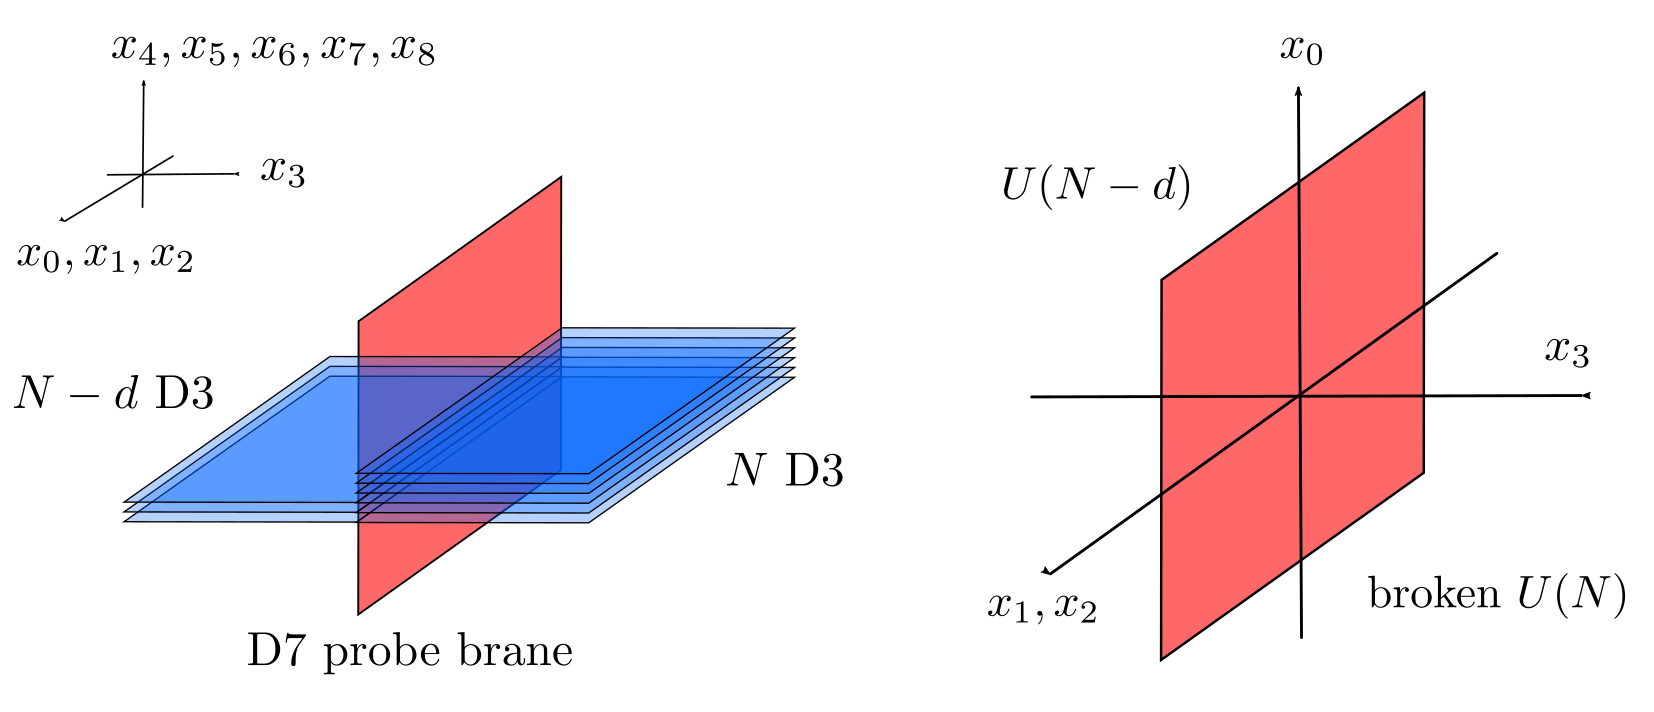
\includegraphics[width=1.0\textwidth]{../pics/brane_vs_field_setup_new.png}
%
\caption[Brane configuration vs. field theory configuration]{The brane configuration in string theory on the left vs. the dual field theory configuration, with different gauge groups on each side of the defect at $x_3=0$, on the right. This figure has been recreated from \cite{One-point functions in D3-D7}.}
%
\label{fig:probe-brane-setup}
%
\end{center}
%
\end{figure}
%
%

\subsection{Symmetries of the dCFTs}
Let us at this point briefly discuss what symmetries of the $\mathcal{N}=4$ SYM field theories survive the introduction of a defect in spacetime. First of all, the presence of the defect quite obviously break translation invariance in the direction perpendicular to itself. Also, the local $U(N - k_1 k_2)$ gauge symmetry in the $x_3 < 0$ region is trivially intact, since we have only zero vevs on this side of the defect. More interesting is the non-zero vevs in the $x_3 > 0$ region, which result from the classical scalar field solutions (\ref{cl solution 1}) and (\ref{cl solution 2}). These vevs partially break both the local $U(N)$ gauge group and the global $PSU(2,2|4)$ super conformal symmetry group of $4D$ $\mathcal{N} = 4$ SYM theory. From the forms of the scalar field solutions, we see that the global $PSU(2,2|4)$ symmetry reduces to the following.
%
%
\begin{equation}
PSU(2,2|4) \to SO(3,2) \times
\begin{cases}
	SO(3) \times SO(3) \\
	SO(5) \\
\end{cases}
\end{equation}
%
%
Where clearly, the upper case corresponds to (\ref{cl solution 1}) vevs, and the lower case corresponds to (\ref{cl solution 2}) vevs. We see that super symmetry is completely broken in these setups, which will become apparent when we look at the mass spectrum of the fields in subsection \ref{diag mass matrix}. The remaining spacetime symmetry is constituted by the Poincar\'e transformations parallel to the defect: $SO(2,1)$, and dilatations of spacetime: $SO(1,1)$, together with special conformal transformations that complete $SO(3,2)$. As already mentioned, the $U(N)$ gauge group is also partially broken by the non zero vevs, and is reduced to the following.
%
%
\begin{equation}
U(N) \to
\begin{cases}
	U(N - k_1 k_2) \times U(1) \times U(1) \\
	U(N - d_n) \times U(1) \\
\end{cases}
\end{equation}
%
%
Where the upper and lower cases again correspond to $\mathfrak{so}(3) \times \mathfrak{so}(3)$ and $\mathfrak{so}(5)$ symmetric vevs respectively. This is easily seen, as only multiples of $\mathbb{1}_{k_1}$, $\mathbb{1}_{k_2}$ commutes with $t_i^{k_1}$, $t_i^{k_2}$ respectively. Similarly, only multiples of $\mathbb{1}_{d_n}$ commutes with $G_{i6}^{d_n}$. Thus, the scalar field solutions $\Phi_i$ commutes with matrices of the form: $U = e^{i \theta_1} \mathbb{1}_{k_1} \otimes e^{i \theta_2} \mathbb{1}_{k_2} \oplus U_{N - k_1 k_2}$, in the $\mathfrak{so}(3) \times \mathfrak{so}(3)$ case, and matrices of the form: $U = e^{i \theta} \mathbb{1}_{d_n} \oplus U_{N - d_n}$, in the $\mathfrak{so}(5)$ case. However, because the gauge group in the $x_3 < 0$ region is given by either $U(N - k_1 k_2)$ or $U(N - d_n)$, any gauge transformation in the $x_3 > 0$ region has to reduce to either $U(N - k_1 k_2)$ or $U(N - d_n)$ transformations at the boundary. This is only possible for the subset of unitary transformations above, for which $\theta_1 = 0$, $\theta_2 = 0$ for the $\mathfrak{so}(3) \times \mathfrak{so}(3)$ case, and $\theta = 0$ for the $\mathfrak{so}(5)$ case. Thus, the gauge group in both cases is further reduced, so that the gauge groups on both sides of the defect agrees.
%
%
\begin{equation}
U(N) \to
\begin{cases}
	U(N - k_1 k_2) \\
	U(N - d_n) \\
\end{cases}
\end{equation}
%
%

\subsection{The aim of the thesis}
The primary focus of this thesis will be to study different kinds of bulk-to-bulk two-point functions in $\mathcal{N} = 4$ defect conformal field theories, with vevs given by either (\ref{cl solution 1}) or (\ref{cl solution 2}). More precisely, we will be looking at two-point functions of various local scalar single-trace operators $\mathcal{O}_a(x)$ and $\mathcal{O}_b(y)$, where the indicies $a$, $b$ label operators of the form.
%
%
\begin{equation}
\mathcal{O}_{a,b}(x) = \Psi_{a,b}^{i_1 \ldots i_L} \tr[\boldsymbol{\phi}_{i_1}(x) \ldots \boldsymbol{\phi}_{i_L}(x)]
%
\quad , \quad
%
x_3,y_3 > 0
\end{equation}
%
%
One-point functions between certain operators of the above types, have already been studied in \cite{One-point functions in D3-D7} for the case of $\mathfrak{so}(3) \times \mathfrak{so}(3)$ symmetric vevs, and in \cite{One-point functions in D3-D7 SO(5)} for the case of $\mathfrak{so}(5)$ symmetric vevs. The techniques developed in \cite{One-point functions in D3-D7,One-point functions in D3-D7 SO(5)} will also be intrumental in computing two-point functions, and so will the ideas presented in \cite{Length L length 2 two-point functions D5-D3}. The structure of this thesis will be as follow. First, in section \ref{sec:dCFT}, we will go through the necessary steps to bring the theory to a form suitable for making perturbatively calculations, of which the biggest challenge is to diagonalize all the new quadratic terms in the Lagrangian. We then proceed, in section \ref{sec:CPO}, to pertubativly compute the leading order contributions to two-point functions of different scalar single-trace chiral primary operators. Lastly, in section \ref{sec:NPO}, we attempt to compute the leading order contribution to the two-point fuctions of a certain type of non-protected operators with definite conformal dimension at 1-loop level, and single-trace scalar operators of length two.

%\subsection{Residual symmetry}
%Representative expressions involving $\Phi_i$ after expansion of action. 
%%
%%
%\begin{equation}
%[\tilde{\phi}_i, \Phi_j]
%%
%\to
%%
%[U \tilde{\phi}_i U^\dagger, \Phi_j]
%%
%=
%%
%U [\tilde{\phi}_i , U^\dagger \Phi_j U] U^\dagger
%\end{equation}
%%
%%
%
%%
%%
%\begin{equation}
%[\Phi_i, \Phi_j]
%%
%\to
%%
%[\Phi_i, \Phi_j]
%%
%=
%%
%U [U^\dagger \Phi_i U , U^\dagger \Phi_j U] U^\dagger
%\end{equation}
%%
%%
%
%%
%%
%\begin{equation}
%D_\mu \Phi_i
%%
%=
%%
%\partial_\mu \Phi_i - i [A_\mu, \Phi_i]
%%
%\to
%%
%\partial_\mu \Phi_i - i [U A_\mu U^\dagger + i U \partial_\mu U^\dagger, \Phi_i]
%\end{equation}
%%
%%
%\begin{equation}
%=
%%
%U \partial_\mu (U^\dagger \Phi_i U) U^\dagger -i U [A_\mu, U^\dagger \Phi U] U^\dagger
%%
%=
%%
%U D_\mu (U^\dagger \Phi_i U) U^\dagger
%\end{equation}
%%
%%
%All is good, so long as:
%%
%%
%\begin{equation}
%U^\dagger \Phi_i U = \Phi_i
%%
%\quad \Rightarrow \quad
%%
%[\Phi_i, U] = 0
%\end{equation}
%%
%%


\newpage

% section 2: The dCFT setup
% \newgeometry{top=4cm,left=4cm,right=4cm,bottom=4cm} 
%
\section{Defect conformal field theory setup}\label{sec:dCFT}
In this section, we go through the ground work necessary for subsequent pertubative calculations in the dCFT setups under consideration. This is essentially a matter of finding the propagators of all fields in the theory, such that they can be used in computing Feynmann diagrams. However, this seemingly straight forward task is vastly complicated by the appearance of a completely scrambled mass-matrix (\textit{this mass-matrix is non diagonal in both color and flavor indices, as we will see later on}). We first look at the particular non trivial solutions of the scalar equations of motion (\textit{EOM's}) in $\mathcal{N} = 4$ SYM theory (\textit{SYM}), that will server as the vacua for our defect conformal field theory setups. The fields of the theory will then acquire masses in the usual Higgs-like manner. After gauge-fixing the $\mathcal{N} = 4$ action and reducing the 10D Majorana-Weyl fermions, we expand around the classical scalar field solutions and find the form of the mass-matrix. Seeing as the procedure of diagonalizing the mass-matrix is a rather long and complicated one, we will not go through all the details in this thesis, but instead refer the reader to the original paper in which this was done \cite{One-point functions in D3-D7}. We conclude this section by finding the propagators of the diagonal fields, which is slightly complicated by the fact that the mass eigenvalues are spacetime dependent.

\subsection{Non zero classical scalar field solutions}\label{cl scalar solutions}
Our starting point for the entire proceeding analysis is the $\mathcal{N}=4$ SYM action, which looks as follow.
%
%
\begin{equation*}
S_{\mathcal{N}=4} = \frac{2}{g^2} \int_{\mathbb{R}^4} \text{d}^4 x
\tr \left[
-\frac{1}{4} (F_{\mu \nu})^2
-\frac{1}{2} (D_\mu \boldsymbol{\phi}_i)^2
+ \frac{i}{2} \bar{\Psi} \Gamma^\mu D_{\mu} \Psi
\right.
\end{equation*}
%
%
\begin{equation}\label{SYM action}
\left.
+ \frac{1}{2} \bar{\Psi} \tilde{\Gamma}^i [\boldsymbol{\phi}_i, \Psi]
+ \frac{1}{4} [\boldsymbol{\phi}_i, \boldsymbol{\phi}_j]^2
\right]
\end{equation}
%
%
%Potential function to be considered:
%%
%%
%\begin{equation}
%V(\{ \phi_i \})
%%
%=
%%
%\tr \left[
%-\partial_\mu \phi_i \partial^\mu \phi^i
%+ \frac{1}{2} [\phi_i, \phi_j] [\phi^i, \phi^j]
%\right]
%\end{equation}
%%
%%
%Where $\mu = 1,...,3$ label coordinates over spacetime, and $i = 1,...,6$ label coordinates in the R-symmetry space. We now decompose the $\phi$ fields in a $U(N)$ basis $\{ T^1, T^a \}$, satisfying:
%%
%%
%\begin{equation}
%\tr \left[ T^a, T^b \right] = \delta^{ab}
%\end{equation}
%%
%%
%\begin{equation}
%\tr \left[ T^1, T^a \right] = 0
%\end{equation}
%%
%%
%\begin{equation}
%\tr \left[ T^1, T^1 \right] = 1
%\end{equation}
%%
%%
%Where $a=2,...,N^2$ and $T^1 = \mathbb{1} / \sqrt{N}$.
%%
%%
%\begin{equation}
%V(\{ \phi_i^1, \phi_i^a \})
%%
%=
%%
%-\partial_\mu \phi_i^1 \partial^\mu \phi^i_1
%-\partial_\mu \phi_i^a \partial^\mu \phi^i_a
%+ ...
%\end{equation}
%%
%%
The field content of the theory is: one $U(N)$ gauge field $A_\mu$, six Lorentz scalars $\boldsymbol{\phi}_i$ and one 10D Majorana-Weyl spinor $\Psi$ (\textit{in section \ref{fermion redution} we explain how to reduce this 10D spinor to four 4D spinors}). The set of matrices $\{\Gamma^\mu , \tilde{\Gamma}^i \}$ constitute 10D gamma matrices. All fields transform in the same representation of $U(N)$ (\textit{as is necessary for the theory to be super symmetric}), namely the adjoint representation\footnote{As for all guage theories, it is not the guage field $A_\mu$ which transforms as an adjoint field, but rather the field strength $F_{\mu\nu}$.}. We use the following conventions for the field strength $F_{\mu\nu}$ and the adjoint covariant derivative $D_\mu$.

\newpage
%
%
\begin{equation}
D_\mu \chi = \partial_\mu \chi - i [A_\mu, \chi]
%
\quad , \quad
%
\chi \in \{F_{\mu\nu}, \Psi, \boldsymbol{\phi}_i \}
\end{equation}
%
%

%
%
\begin{equation}
F_{\mu\nu} = \partial_\mu A_\nu - \partial_\nu A_\mu -i [A_\mu, A_\nu]
\end{equation}
%
%
We now look for solutions to the EOM's of this action, such that the scalar fields $\boldsymbol{\phi}_i$, are non-zero while all other fields vanish. We can now vary the action with respect to the scalars, and assuming all other fields vanish we find that.
%
%
\begin{equation}\label{Scalar Field EOMS}
\frac{\delta S_{\mathcal{N} = 4}}{\delta \boldsymbol{\phi}_i} = 0
%
\quad \Rightarrow \quad
%
\partial_\mu \partial^\mu \boldsymbol{\phi}_i
=
[\boldsymbol{\phi}_j, [\boldsymbol{\phi}_j, \boldsymbol{\phi}_i]]
\end{equation}
%
%
%A solution to these equations are given by the following.
%%
%%
%\[ \Phi^i_R(x) = -\frac{1}{x_3} t_R^i = -\frac{1}{x_3}
%	\begin{cases}
%		t_1^i \oplus 0_{N-k_1}
%		& \quad \text{for } i = 1,2,3 \\
%		
%    	0_{N-k_2} \oplus t_2^{i-3}
%    	& \quad \text{for } i = 4,5,6
%  \end{cases}
%\]
%%
%%
%Where $t_1^i$ and $t_2^i$ are $k_1$ and $k_2$ dimensional representations of the $\mathfrak{su}(2)$ generators respectivly, and $k_1 + k_2 \leq N$.
A non-zero solution to these equations was presented in \cite{One-point functions in D3-D7}. The solution has the following form.
%
%
\begin{equation*}
\mathfrak{so}(3) \times \mathfrak{so}(3) :
%
\quad
%
\Phi_i(x)
=
-\frac{1}{x_3}
	\begin{cases}
		t_i^{(1)} \oplus 0_{N-k_1 k_2}
		& \quad \text{for } i = 1,2,3 \\
		
    	t_{i-3}^{(2)} \oplus 0_{N-k_1 k_2}
    	& \quad \text{for } i = 4,5,6
  \end{cases}
\quad ,
\end{equation*}
%
%
\begin{equation}\label{cl solution a}
t_i^{(1)} \equiv t_i^{k_1} \otimes \mathbb{1}_{k_2}
%
\quad , \quad
t_i^{(2)} \equiv \mathbb{1}_{k_1} \otimes t_i^{k_2}
\end{equation}
%
%
Here, $t_i^{k_1}$ and $t_i^{k_2}$ are $k_1$ and $k_2$ dimensional representations of the $\mathfrak{so}(3)$ generators respectively, and $k_1 k_2 \leq N$. It is easy to verify that this is indeed a solution of equ. (\ref{Scalar Field EOMS}) using the $\mathfrak{so}(3)$ commutation relations: $[t_i, t_j] = i \varepsilon_{ijk} t_k$, and the identity: $\varepsilon_{jkl} \varepsilon_{jik} = -2 \delta_{li}$.
%
%
\begin{equation}\label{double commutator so(3)}
[t_j, [t_j, t_i]] = i \varepsilon_{jik} [t_j, t_k]
=
-\varepsilon_{jik} \varepsilon_{jkl} t_l
=
2 t_i
%
\quad , \quad
%
i,j,k,l = 1,2,3
\end{equation}
%
%
Using the result in (\ref{double commutator so(3)}) and the fact that $t_i^{k_1} \otimes \mathbb{1}_{k_2}$ and $\mathbb{1}_{k_1} \otimes t_{j}^{k_2}$ commute, it should be clear that (\ref{cl solution a}) is indeed a solution to (\ref{Scalar Field EOMS}). It should be noted at this point, that a certain limit of this solution (\textit{$k_1 = 1$ or $k_2 = 1$}) is dual to the so called fuzzy-funnel solution of the probe D5-D3 brane setup with $AdS_4 \times S^2$ geometry \cite{fuzzy-funnel solution}.\\
% Certainly, something similar must exist for the general case
In addition to the above classical field solution, another non-zero solution also exists \cite{One-point functions in D3-D7 SO(5)}, and it is given by the following similar looking expression.
%
%
\begin{equation}\label{cl solution b}
\mathfrak{so}(5) :
%
\quad
%
\Phi_i(x)
=
\frac{1}{\sqrt{2} x_3}
	\begin{cases}
		G_{i6}^{d_n} \oplus 0_{N-d_n}
		& \quad \text{for } i = 1,2,3,4,5 \\
		
    	0_{N}
    	& \quad \text{for } i = 6
  \end{cases}
\end{equation}
%
%
Where $G_{i6}^{d_n}$ are a subset of the $d_n = d_6 \left(\frac{n}{2},\frac{n}{2},\frac{n}{2} \right)$ dimensional representations of $\mathfrak{so}(6)$ generators. It is again easy to verify that the above is indeed a solution of (\ref{Scalar Field EOMS}), this time using the commutation relations of $\mathfrak{so}(6)$ and the fact that $G_{ij} = -G_{ji}$.

\newpage
%
%
\begin{equation*}
[G_{ij}, G_{kl}] = i \left(
\delta_{ik} G_{jl}
+ \delta_{jl} G_{ik}
- \delta_{il} G_{jk}
- \delta_{jk} G_{il}
\right)
%
\quad ,
\end{equation*}
%
%
\begin{equation}
i,j,k,l = 1, \ldots 6
\end{equation}
%
%
\begin{equation}
[G_{j6}, G_{i6}] = i G_{ji}
%
\quad , \quad
%
i,j,k,l = 1, \ldots 5
\end{equation}
%
%
\begin{equation*}
[G_{j6}, [G_{j6}, G_{i6}]] = i [G_{j6}, G_{ji}]
=
-\left(
\delta_{jj} G_{6i}
- \delta_{ji} G_{6j}
\right)
=
4 G_{i6}
%
\quad ,
\end{equation*}
%
%
\begin{equation}\label{double commutator so(5)}
i,j,k,l = 1, \ldots 5
\end{equation}
%
%
Using the result (\ref{double commutator so(5)}), it should again be clear that (\ref{cl solution b}) is indeed also a solution to equ. (\ref{Scalar Field EOMS}). It should again be noted, that this solution is also dual to a fuzzy-funnel solution, this time of the probe D7-D3 brane setup with $AdS_4 \times S^4$ geometry \cite{fuzzy-funnel solution D7}.

\subsection{Reducing the 10D Majorana-Weyl fermion}\label{fermion redution}
When we presented the fields of $\mathcal{N} = 4$ SYM back in section \ref{cl scalar solutions}, one field might have seemed a bit out of place; namely the $10D$ Majorana-Weyl fermion. This $10D$ fermion is in fact a remnant of the $10D$ $\mathcal{N} = 1$ SYM action, from which we can obtain the $4D$ $\mathcal{N} = 4$ action by dimensional reduction. For the sake of completness, we present here the $\mathcal{N} = 1$ SYM action.
%
%
\begin{equation}
S_{\mathcal{N}=1} = \frac{2}{\tilde{g}^2} \int_{\mathbb{R}^{10}} \text{d}^{10} x
\tr \left[
-\frac{1}{4} (F_{M N})^2
+ \frac{i}{2} \bar{\Psi} \Gamma^M D_{M} \Psi
\right]
%
\quad , \quad
%
M,N = 0,...,9
\end{equation}
%
%
Where $\bar{\Psi} \equiv \Psi^\dagger \Gamma^0$. We now move on to the task of decomposing the $10D$ Majorana-Weyl fermion into a set of $4D$ fermions. To do this, we need to take into account both the Majorana and Weyl constraints for the $10D$ Majorana-Weyl fermion.
%
%
\begin{equation}\label{10 Weyl-Majorana}
\Psi = \Psi^C \equiv \mathcal{C}_{10} \Gamma^0  \Psi^{*}
%
\quad , \quad
%
\Gamma^{11} \Psi = -\Psi
\end{equation}
%
%
Where $\Gamma^M$, $\Gamma^{11}$ are $10D$ gamma matrices, which have to obey the Clifford anti-commutator algebra.
%
%
\begin{equation}
\{ \Gamma^M, \Gamma^N \} = -2 \eta^{MN}
%
\quad , \quad
%
\Gamma^{11} = i \, \Gamma^0 \cdots \Gamma^9
\end{equation}
%
%
In the above, $C_{10}$ is the $10D$ charge conjugation matrix, which implicitly defined by the following relation: $-\left( {\Gamma^M} \right)^{*} = \Gamma^0 \, C_{10}^{-1} \, \Gamma^M \, C_{10} \, \Gamma^0$. In what follows, we will employ the representation of $10D$ gamma matrices and the $10D$ charge conjugation matrix given below.

\newpage
%
%
\begin{equation}\label{Gamma_mu}
\Gamma^\mu = \gamma^\mu \otimes \mathbb{1}_4 \otimes \mathbb{1}_2
%
\quad , \quad
%
\mu = 0,1,2,3
\end{equation}
%
%

%
%
\begin{equation}\label{Gamma_i}
\tilde{\Gamma}^i \equiv \Gamma^{i+3} =
	\begin{cases}
		-i \, \gamma^5 \otimes G^i \otimes \sigma_2
		& \quad \text{for } i = 1,2,3 \\
		
    	\gamma^5 \otimes G^i \otimes \sigma_1
    	& \quad \text{for } i = 4,5,6
  \end{cases}
\end{equation}
%
%

%
%
\begin{equation}
\Gamma^{11} = -\gamma^5 \otimes \mathbb{1}_4 \otimes \sigma_3
\end{equation}
%
%

%
%
\begin{equation}
C_{10} = C_4 \otimes \mathbb{1}_4 \otimes \sigma_1
%
\quad , \quad
%
C_4 = i \, \sigma_2 \otimes \sigma_3
\end{equation}
%
%
Where the $4 \times 4$ matrices $G^i$ are given by the following expressions.
%
%
\begin{equation*}
G^1 = \sigma_3 \otimes \sigma_2
%
\quad , \quad
%
G^2 = -\sigma_2 \otimes \sigma_2 
%
\quad , \quad
%
G^3 = \sigma_2 \otimes \mathbb{1}_2
\end{equation*}
%
%
\begin{equation}
G^4 = -i \, \sigma_2 \otimes \sigma_1
%
\quad , \quad
%
G^5 = -i \, \mathbb{1}_2 \otimes \sigma_2
%
\quad , \quad
%
G^6 = i \, \sigma_2 \otimes \sigma_3
\end{equation}
%
%
And the $4 \times 4$ matrices $\gamma^\mu$, $\gamma^5$ are given by the following expressions.
%
%
\begin{equation*}
\gamma^\mu = \left( \begin{array}{cc}
0 & \sigma^\mu \\
\bar{\sigma}^\mu & 0
\end{array} \right)
%
\quad , \quad
%
\gamma^5 = i \, \gamma^0 \cdots \gamma^3
%
\quad ,
\end{equation*}
%
%
\begin{equation}
\sigma^\mu = (\mathbb{1}_2, \sigma^i)
%
\quad , \quad
%
\bar{\sigma}^\mu = (\mathbb{1}_2, -\sigma^i)
\end{equation}
%
%
We start now with an unconstrained $10D$ Dirac fermion. The way we have expressed the $10D$ gamma matrices suggest a decomposition into two blocks of four $4D$ fermions. We therefore write out the $10D$ fermion in the following way.
%
%
\begin{equation}\label{unconstrained spinor}
\Psi = \left( \begin{array}{c}
\chi_1 \\
\vdots \\
\chi_4 \\
\chi_5 \\
\vdots \\
\chi_8
\end{array} \right)
\end{equation}
%
%
Where the $\chi$'s are unconstrained $4D$ Dirac fermions. The Weyl condition in equ. (\ref{10 Weyl-Majorana}) amounts to the following when applied to the $10D$ Dirac spinor (\ref{unconstrained spinor}).

\newpage
%
%
\begin{equation}\label{after Weyl imposed}
\left( \begin{array}{c}
\chi_1 \\
\vdots \\
\chi_4 \\
\chi_5 \\
\vdots \\
\chi_8
\end{array} \right)
%\text{d}^4 x
=
%
\left( \begin{array}{c}
+ \gamma_5 \chi_1 \\
\vdots \\
+ \gamma_5 \chi_4 \\
- \gamma_5 \chi_5 \\
\vdots \\
- \gamma_5 \chi_8
\end{array} \right)
%
\quad \Rightarrow \quad
%
\left( \begin{array}{c}
\chi_1 \\
\vdots \\
\chi_4 \\
\chi_5 \\
\vdots \\
\chi_8
\end{array} \right)
%
=
%
\left( \begin{array}{c}
L \psi_1 \\
\vdots \\
L \psi_4 \\
R \psi_5 \\
\vdots \\
R \psi_8
\end{array} \right)
\end{equation}
%
%
Where $L = \frac{\mathbb{1}_4 + \gamma_5}{2}$ and $R = \frac{\mathbb{1}_4 - \gamma^5}{2}$ are standard projection operators, and the $\psi$'s are new unconstrained $4D$ Dirac fermions. The Majorana condition in equ. (\ref{10 Weyl-Majorana}) amounts to the following when applied to the result in (\ref{after Weyl imposed}).
%
%
\begin{equation*}
\left( \begin{array}{c}
L \psi_1 \\
\vdots \\
L \psi_4 \\
R \psi_5 \\
\vdots \\
R \psi_8
\end{array} \right)
%
=
%
\left( \begin{array}{c}
C_4 \gamma^0 R \psi_5^{*} \\
\vdots \\
C_4 \gamma^0 R \psi_8^{*} \\
C_4 \gamma^0 L \psi_1^{*} \\
\vdots \\
C_4 \gamma^0 L \psi_4^{*}
\end{array} \right)
%
=
%
\left( \begin{array}{c}
R \psi_5^{C} \\
\vdots \\
R \psi_8^{C} \\
L \psi_1^{C} \\
\vdots \\
L \psi_4^{C}
\end{array} \right)
%
\end{equation*}
%
%
\begin{equation}
\Rightarrow \quad
%
\left( \begin{array}{c}
L \psi_1 \\
\vdots \\
L \psi_4 \\
R \psi_5 \\
\vdots \\
R \psi_8
\end{array} \right)
%
=
%
\left( \begin{array}{c}
L \psi_1 \\
\vdots \\
L \psi_4 \\
R \psi_1 \\
\vdots \\
R \psi_4
\end{array} \right)
\end{equation}
%
%
Where we have used that $C_4 \, \gamma^0 \, \gamma^5 \, \psi_i^{*} = -C_4 \, \gamma^0 \, \gamma^5 \, \gamma^0 \, C_4 \, \psi_i^{C} = -\gamma^5 \, \psi_i^{C}$, and concluded that the $4D$ spinors $\psi_i$ with $a=1,2,3,4$, must be Majorana spinors: $\psi_i = \psi_i^{C} \equiv \mathcal{C}_{4} \, \gamma^0 \, \psi_i^{*}$.\\
Now that we know how the $10D$ Majorana-Weyl fermion splits into four left-chiral and four right-chiral $4D$ Majorana fermions, we can use this information to figure out how the terms in the $\mathcal{N} = 4$ action (\ref{SYM action}), involving the Majorana-Weyl fermion, reduce. The terms in question are the following.
%
%
\begin{equation}
\frac{i}{2} \bar{\Psi} \Gamma^M D_M \Psi
%
\xlongrightarrow{\makebox[2cm]{ Dim. Red. }}
%
\frac{i}{2} \bar{\Psi} \Gamma^\mu D_{\mu} \Psi
+
\frac{1}{2} \bar{\Psi} \tilde{\Gamma}_i [\boldsymbol{\phi}_i, \Psi]
\end{equation}
%
%
Because of the simple sctructure of the $\Gamma^\mu$ matrices, given in equ. (\ref{Gamma_mu}), we find that the kinetic term of the Majorana-Weyl spinor reduce in the following simple way.
%
%
\begin{equation}
\frac{i}{2} \bar{\Psi} \Gamma^\mu D_{\mu} \Psi
=
\frac{i}{2} (L \psi_a)^\dagger \gamma^0 \gamma^\mu D_{\mu} L \psi^a
+
\frac{i}{2} (R \psi_a)^\dagger \gamma^0 \gamma^\mu D_{\mu} R \psi^a
=
\frac{i}{2} \bar{\psi_a} \gamma^\mu D_{\mu} \psi^a
\end{equation}
%
%
Where we have used that $L$, $R$ are Hermitian, $\{ \gamma^5, \gamma^\mu \} = 0$ and the simple property: $L \psi + R \psi = \psi$. We have also made use of the definition: $\bar{\psi} \equiv \psi^\dagger \gamma_0$. In reducing the fermion-scalar interaction term, the simple struture of the gamma matrices, this time  $\tilde{\Gamma}^i$ (\ref{Gamma_i}), again simplify the procedure.
%
%
\begin{equation*}
\frac{1}{2} \bar{\Psi} \tilde{\Gamma}_i [\boldsymbol{\phi}_i, \Psi]
=
\end{equation*}
%
%
\begin{equation*}
\sum_{i=1}^3 \frac{1}{2} (R \psi_a)^\dagger \gamma^0 \gamma^5 {(G_i)^a}_b [\boldsymbol{\phi}_i, L \psi^b]
-
\sum_{i=1}^3 \frac{1}{2} (L \psi_a)^\dagger \gamma^0 \gamma^5 {(G_i)^a}_b [\boldsymbol{\phi}_i, R \psi^b]
\end{equation*}
%
%
\begin{equation*}
+
\sum_{i=4}^6 \frac{1}{2} (R \psi_a)^\dagger \gamma^0 \gamma^5 {(G_i)^a}_b [\boldsymbol{\phi}_i, L \psi^b]
+
\sum_{i=4}^6 \frac{1}{2} (L \psi_a)^\dagger \gamma^0 \gamma^5 {(G_i)^a}_b [\boldsymbol{\phi}_i, R \psi^b]
\end{equation*}
%
%
\begin{equation}
=
\sum_{i=1}^3 \frac{1}{2} \bar{\psi_a} {(G_i)^a}_b [\boldsymbol{\phi}_i, \psi^b]
+
\sum_{i=4}^6 \frac{1}{2} \bar{\psi_a} {(G_i)^a}_b [\boldsymbol{\phi}_i, \gamma^5 \psi^b]
\end{equation}
%
%
Where we have used the same properties to simplify as we did for the kinetic term, and additionally $L \, \gamma^5 = L$ and $R \, \gamma^5 = -R$. With both the kinetic and the interaction term reduced, we finally have the spinor terms in a form appropriate for extracting propagators and vertex rules for the fields in our dCFT setups. As a last aside for this section, we note that the ${(G_i)^a}_b$ matrices are related to (\textit{Euclidian}) $6D$ gamma matrices. In our conventions, these gamma matrices would take the forms:
%
%
\begin{equation}
\gamma^{(6)}_i
=
\begin{cases}
	-i \, G_i \otimes \sigma_2
	& \quad \text{for } i = 1,2,3 \\
		
    G_i \otimes \sigma_1
    & \quad \text{for } i = 4,5,6 \\
\end{cases}
\end{equation}
%
%

\subsection{Gauge fixing and ghost fields}\label{gauge-fixing}
In order to simplify the diagonilazation of the mass matrix of the spontaneously broken theory (\textit{more on that in section \ref{diag mass matrix}}), we want to get rid of the terms in the expanded action (\ref{expanded action}) quadritic in the fields and containing a derivative. We will see in section \ref{fluct cl} that one such term appears, and has the form.
%
%
\begin{equation}\label{unwanted term}
\tr[i [A_\mu, \Phi_i] \partial^\mu \phi_i]
%
\quad \text{ with } \quad
%
\boldsymbol{\phi}_i = \Phi_i + \phi_i
\end{equation}
%
%
It turns out we can get rid of this term by gauge-fixing in a clever way \cite{One-point functions in D5-D3}; effectively killing two birds with one stone. To be more precise, we choose to gauge-fix the action (\ref{SYM action}) using the following gauge-fixing function.
%
%
\begin{equation*}
G[A_\mu,\boldsymbol{\phi}_i] = \partial_\mu A^\mu + i [\boldsymbol{\phi}_i, \Phi_i]
%
\quad ,
\end{equation*}
%
%
\begin{equation}
S_{\text{gf}} = \frac{2}{g^2} \int_{\mathbb{R}^4} \text{d}^4 x
\tr \left[
-\frac{1}{2 \xi} G[A_\mu, \boldsymbol{\phi}_i]^2
\right]
\end{equation}
%
%
Where $S_{\text{gf}}$ is an extra term, which appears in the action after performing the \textit{Faddev-Popov gauge-fixing procedure}. The slightly unusual thing about the gauge-fixing function above, is the fact that it depends also on the scalar fields $\boldsymbol{\phi}_i$ in addition to the gauge fields $A_\mu$. By looking at the form of (\ref{unwanted term}), it should however be fairly obvious that we need the $\boldsymbol{\phi}_i$ dependence in the gauge-fixing function, if there is to be any hope of canceling this unwanted term.\\
In what follows, we will always work in the gauge for which $\xi = 1$. We can now insert our gauge-fixing function into $S_{\text{gf}}$. The result is the following.
\begin{equation*}
S_{\text{gf}} = \frac{2}{g^2} \int_{\mathbb{R}^4} \text{d}^4 x
\tr \left[
-\frac{1}{2}
(\partial_\mu A^\mu)^2
- [\boldsymbol{\phi}_i, \Phi_i]^2
+ 2 i [\boldsymbol{\phi}_i, \Phi_i] \partial_\mu A^\mu
\right]
\end{equation*}
%
%
\begin{equation}
=
%
\frac{2}{g^2} \int_{\mathbb{R}^4} \text{d}^4 x
\tr \bigg[
-\frac{1}{2} (\partial_\mu A^\mu)^2
+ \frac{1}{2} [\phi_i, \Phi_i]^2
+ i [\partial_\mu \phi_i, \Phi_i] A^\mu
+ i [\phi_i, \partial_\mu \Phi_i] A^\mu
\bigg]
\end{equation}
%
%
Where we have used integration by parts to get the second equality. It can easily be seen (\textit{using the cylic property of the trace operation}) that the third term in the above gauge-fixing action exactly cancels the unwanted term (\ref{unwanted term}). As usual, the first term in the gauge-fixing action cancels the problematic part of the kinetic term for the $A_\mu$ fields, leaving an invertible and diagonal term.\\
Now we turn our attention to the ghost part of the action. Under a infinitesimal gauge tranformation, $A_\mu$ and $\boldsymbol{\phi}_i$ transform in the following ways.
%
%
\begin{equation}
\delta A_\mu = D_\mu \varepsilon = \partial_\mu \varepsilon - i [A_\mu, \varepsilon]
%
\quad , \quad
%
\delta \boldsymbol{\phi}_i = -i [\boldsymbol{\phi}_i, \varepsilon]
\end{equation}
%
%
The ghost part of the action $S_{\text{gh}}$ can then be extracted from the following functional determinant.
%
%
\begin{equation}
\text{det} \left(
\frac{\delta G[A_\mu + D_\mu \varepsilon, \boldsymbol{\phi}_i - i[\boldsymbol{\phi}_i, \varepsilon]]}{\delta \varepsilon}
\right)
=
\text{det} \left(
\partial^\mu D_\mu [\; \cdot \; ]
- [\Phi_i, [\Phi_i + \phi_i, \; \cdot \; ]]
\right)
\end{equation}
%
%
Where the $[ \; \cdot \;]$ denote an unfilled argument of an operator. We can now make use of the fact that the functional determinant of any operator $\mathcal{O}$ can be written as a Grassman path integral as follow.
%
%
\begin{equation}
\text{det} ( \mathcal{O} )
%
=
%
\int \mathcal{D} \bar{c} \, \mathcal{D}c \exp
\left(
i \, \frac{2}{g^2} \int_{\mathbb{R}^4} \text{d}^4 x
\trace \left[ \bar{c} \, \mathcal{O} \, c \right]
\right)
\end{equation}
%
%
\begin{equation}
\Rightarrow \quad
%
S_{\text{gh}} = \frac{2}{g^2} \int_{\mathbb{R}^4} \text{d}^4 x
\tr \left[
\bar{c} \, \partial^\mu D_\mu c
- \bar{c} \, [\Phi_i, [\Phi_i + \phi_i, c]]
\right]
\end{equation}
%
%
The prefactor of $2 / g^2$ is of course purely conventional. We now see the price we have to pay to get rid of the unwanted term (\ref{unwanted term}); namely the appearance of massive ghosts which couple directly to the scalar fields. Nevertheless, we can now write the full gauge-fixed actions with Faddeev-Popov ghosts.
%
%
\begin{equation}
S = S_{\mathcal{N} = 4} + S_{\text{gf}} + S_{\text{gh}}
\end{equation}
%
%
Where the $\mathcal{N}=4$ super Yang Mills action $S_{\mathcal{N} = 4}$ is given in equ. (\ref{SYM action}) in the previous section \ref{cl scalar solutions}.

\subsection{Fluctuations around the classical scalar solutions}\label{fluct cl}
Now that we have managed to both gauge fix the action (\textit{in a way which will simplify the mass matrix diagonalization}) and reduce the $10D$ Majorana-Weyl fermion, we are now ready to expand the six scalar fields $\boldsymbol{\phi}_i$ around the classical solutions (\ref{cl solution a}), (\ref{cl solution b}) and find the effective form of the action (\ref{SYM action}). We first write the scalar fields as follow.
%
%
\begin{equation}
\boldsymbol{\phi}_i = \Phi_i + \phi_i
\end{equation}
%
%
Where $\phi_i$ are perturbations around the classical solutions. Before we get further into the process of expanding the $\mathcal{N} = 4$ action, we note the following two things. Firstly, the field independent part of the expanded action.
%
%
\begin{equation}
\frac{1}{2} \Phi_i \, \partial^\mu \partial_\mu \Phi_i
- \frac{1}{4} \Phi_i [\Phi_j, [\Phi_j, \Phi_i]]
\end{equation}
%
%
Will be ignored from now on, as it does not affect any perturbative calculations. Secondly, the part of the expanded action linear in $\phi_i$ will vanish due to the EOM's for the scalar fields.
%
%
\begin{equation}
\phi_i \, \partial^\mu \partial_\mu \Phi_i
- \phi_i \, [\Phi_j, [\Phi_j, \Phi_i]]
= 0
\end{equation}
%
%
We can thus ignore these two terms when expanding the action.
%%\text{d}^4 x
%%
%\begin{equation}
%\tr \left[ 
%\partial_\mu {\phi^{cl}}_i \partial^\mu {\phi^{cl}}^i
%\right]
%%
%=
%%
%\frac{6}{x_3^4} 
%\end{equation}
%%
%%
%
%%
%%
%\begin{equation}
%\tr \left[ 
%[{\phi^{cl}}_i, {\phi^{cl}}_j]
%[{\phi^{cl}}^i, {\phi^{cl}}^j]
%\right]
%%
%=
%%
%\frac{6}{x_3^4} 
%\end{equation}
%%
%%
Let us now start by expanding the kinetic term for the $\phi_i$ fields. We write here the covariant derivate of $\Phi_i$ and $\phi_i$ for convenience.
%
%
\begin{equation}
D_\mu \Phi_i = \partial_\mu \Phi_i -i [A_\mu, \Phi_i]
%
\quad , \quad
%
D_\mu \phi_i = \partial_\mu \phi_i -i [A_\mu, \phi_i]
\end{equation}
%
%
It is now straight forward to expand the kinetic term for the $\phi_i$ fields, the result of which looks as follow.
%
%
\begin{equation*}
\tr \left[ -\frac{1}{2} D_\mu \boldsymbol{\phi}_i D^\mu \boldsymbol{\phi}_i \right]
%
=
%
\tr \left[
- \frac{1}{2} D_\mu \Phi_i D^\mu \Phi_i
- D_\mu \phi_i D^\mu \Phi_i
-\frac{1}{2} D_\mu \phi_i D^\mu \phi_i
\right]
\end{equation*}
%
%
\begin{equation*}
=
\tr \left[
i [A_\mu, \Phi_i] \, \partial^\mu \Phi_i
+ \frac{1}{2} [A_\mu, \Phi_i] [ A^\mu, \Phi_i]
+ i [A_\mu, \Phi_i] \, \partial^\mu \phi_i
+ i [A_\mu, \phi_i] \, \partial^\mu \Phi_i
\right.
\end{equation*}
%
%
\begin{equation}
\left.
+ [A_\mu, \phi_i] [A^\mu, \Phi_i]
- \frac{1}{2} \partial_\mu \phi_i \, \partial^\mu \phi_i
+ i [A_\mu, \phi_i] \, \partial^\mu \phi_i
+ \frac{1}{2} [A_\mu, \phi_i] [A^\mu, \phi_i]
\right]
\end{equation}
%
%
Notice that the problematic term mentioned back in section \ref{gauge-fixing} appears in the above expansion. Notice also that the term linear in $A_\mu$ will only ever be relevant in the computation of one-point function of said field, and we will therefore ignore it from this point on. Next up, we expand the self interaction term for the $\phi_i$ fields, and the $\phi_i$, $\psi$ interaction terms.
%
%
\begin{equation*}
\tr \left[
\frac{1}{4} [\boldsymbol{\phi}_i, \boldsymbol{\phi}_j][\boldsymbol{\phi}_i, \boldsymbol{\phi}_j]
\right]
=
\tr \left[
\frac{1}{4} [\Phi_i, \Phi_j][\Phi_i, \Phi_j]
+ [\phi_i, \Phi_j][\Phi_i, \Phi_j]
+ \frac{1}{2} [\phi_i, \phi_j][\Phi_i, \Phi_j]
\right.
\end{equation*}
%
%
\begin{equation}
\left.
+ \frac{1}{2} [\phi_i, \Phi_j][\phi_i, \Phi_j]
+ \frac{1}{2} [\phi_i, \Phi_j][\Phi_i, \phi_j]
+ [\phi_i, \phi_j][\phi_i, \Phi_j]
+ \frac{1}{4} [\phi_i, \phi_j][\phi_i, \phi^j]
\right]
\end{equation}
%
%

%
%
\begin{equation*}
\tr \left[
\sum_{i=1}^3 \frac{1}{2} \bar{\psi_a} {(G_i)^a}_b [\boldsymbol{\phi}_i, \psi^b]
+
\sum_{i=4}^6 \frac{1}{2} \bar{\psi_a} {(G_i)^a}_b [\boldsymbol{\phi}_i, \gamma^5 \psi^b]
\right]
\end{equation*}
%
%
\begin{equation*}
= 
\tr \left[
\sum_{i=1}^3 \left(
\frac{1}{2} \bar{\psi_a} {(G_i)^a}_b [\Phi_i, \psi^b]
+
\frac{1}{2} \bar{\psi_a} {(G_i)^a}_b [\phi_i, \psi^b]
\right)
\right.
\end{equation*}
%
%
\begin{equation}
\left.
+
\sum_{i=4}^6 \left(
\frac{1}{2} \bar{\psi_a} {(G_i)^a}_b [\Phi_i, \gamma^5 \psi^b]
+
\frac{1}{2}  \psi^b] \bar{\psi_a} {(G_i)^a}_b [\phi_i, \gamma^5
\right)
\right]
\end{equation}
%
%
Now that we have expanded the terms in the $\mathcal{N} = 4$ action involving the $\phi_i$ fields, we can finally write down the entire expanded action in a well organized form.
%
%
\begin{equation}\label{expanded action}
S_{\mathcal{N}=4} = S_{\text{kinetic}} + S_{\text{m,b}} + S_{\text{m,f}}
+ S_{\text{qubic}} + S_{\text{quadratic}}
\end{equation}
%
%

%
%
\begin{equation}
S_{\text{kinetic}}
=
\frac{2}{g^2} \int_{\mathbb{R}^4} \text{d}^4 x
\tr \bigg[
\frac{1}{2} A_\mu \partial_\nu \partial^\nu A^\mu
+ \frac{1}{2} \phi_i \partial_\nu \partial^\nu \phi_i
+ \frac{i}{2} \bar{\psi}_a \gamma^\mu \partial_\mu \psi^a
+ \bar{c} \, \partial_\nu \partial^\nu c
\bigg]
\end{equation}
%
%

%
%
\begin{equation*}
S_{\text{m,b}}
=
\frac{2}{g^2} \int_{\mathbb{R}^4} \text{d}^4 x
\tr \bigg[
\frac{1}{2} [A_\mu, \Phi_i] [ A^\mu, \Phi_i]
+ 2 i [A_\mu, \phi_i] \, \partial^\mu \Phi_i
+ \frac{1}{2} [\phi_i, \phi_j][\Phi_i, \Phi_j]
\end{equation*}
%
%
\begin{equation}\label{boson mass terms}
+ \frac{1}{2} [\phi_i, \Phi_j][\phi_i, \Phi_j]
+ \frac{1}{2} [\phi_i, \Phi_j][\Phi_i, \phi_j]
+ \frac{1}{2} [\phi_i, \Phi_i] [\phi_j, \Phi_j]
\bigg]
\end{equation}
%
%

%
%
\begin{equation*}
S_{\text{m,f}}
=
\frac{2}{g^2} \int_{\mathbb{R}^4} \text{d}^4 x
\tr \bigg[
\sum_{i=1}^3 \frac{1}{2} \bar{\psi_a} {(G_i)^a}_b [\Phi_i, \psi^b]
+
\sum_{i=4}^6 \frac{1}{2} \bar{\psi_a} {(G_i)^a}_b [\Phi_i, \gamma^5 \psi^b]
\end{equation*}
%
%
\begin{equation}\label{fermion mass terms}
-
\bar{c} \, [\Phi_i, [\Phi_i, c]]
\bigg]
\end{equation}
%
%

%
%
\begin{equation*}
S_{\text{cubic}}
=
\frac{2}{g^2} \int_{\mathbb{R}^4} \text{d}^4 x
\tr \bigg[
i [A_\mu, A_\nu] \, \partial^\mu A_\nu
+
[A_\mu, \phi_i] [A^\mu, \Phi_i]
+
i [A_\mu, \phi_i] \, \partial^\mu \phi_i
\end{equation*}
%
%
\begin{equation*}
+
\frac{1}{2} \bar{\psi}_a \gamma^\mu [A_\mu, \psi^a]
+
\sum_{i=1}^3 \frac{1}{2} \bar{\psi_a} {(G_i)^a}_b [\phi_i, \psi^b]
+
\sum_{i=4}^6 \frac{1}{2} \bar{\psi_a} {(G_i)^a}_b [\phi_i, \gamma^5 \psi^b]
\end{equation*}
%
%
\begin{equation}
+
i \, ( \partial^\mu \bar{c} ) [A_\mu, c]
-
\bar{c} \, [\Phi_i, [\phi_i, c]]
+
[\phi_i, \phi_j][\phi_i, \Phi_j]
\bigg]
\end{equation}
%
%

%
%
\begin{equation*}
S_{\text{quartic}}
=
\frac{2}{g^2} \int_{\mathbb{R}^4} \text{d}^4 x
\tr \bigg[
\frac{1}{4} [A_\mu, A_\nu] [A^\mu, A^\nu]
+
\frac{1}{2} [A_\mu, \phi_i] [A^\mu, \phi_i]
\end{equation*}
%
%
\begin{equation}
+
\frac{1}{4} [\phi_i, \phi_j] [\phi_i, \phi_j]
\bigg]
\end{equation}
%
%
Where in the above, we have also included the terms from the gauge-fixing and ghost parts of the action (\textit{see section \ref{gauge-fixing}}), as well as the expanded forms of the kinetic terms for both the $A_\mu$ and $\psi^a$ fields (\textit{see equ. (\ref{SYM action}) for the unexpanded forms}). 

\subsection{Diagonalizing the mass matrix}\label{diag mass matrix}
Now that we finally have the $\mathcal{N} = 4$ SYM action in the fully operational form given above, we are ready to tackle the problem of diagonalizing the mass terms of said action. Looking at both the bosonic (\ref{boson mass terms}) and fermionic (\ref{fermion mass terms}) mass terms of the action (\ref{expanded action}), we see that all of these are either non-diagonal with regards to the $U(N)$ matrix structure (\textit{color mixing}), non-diagonal with regards to the species of fields (\textit{flavor mixing}) or both. The techniques necessary to solve this diagonalization problem was first presented in \cite{One-point functions in D3-D7} for the case of $\mathfrak{so}(3) \times \mathfrak{so}(3)$ symmetric vevs, and in \cite{One-point functions in D3-D7 SO(5)} for the case of $\mathfrak{so}(5)$ symmetric vevs. The following subsection will constitute a review of the work contained in those aforementioned articles.

\subsubsection[Boson mass matrix: $SO(3) \times SO(3)$ symmetric vevs]{Boson mass matrix: $\mathbf{SO(3) \times SO(3)}$ symmetric vevs}
In order to more clearly see the structure which makes the diagonalization of the boson mass matrix possible, we have to work a bit witht the form of $S_{\text{m,b}}$. It turns out that we can rewrite the boson mass part of the total action (\ref{boson mass terms}) to the following.
%
%
\begin{equation*}
S_{\text{m,b}}
=
\frac{2}{g^2} \int_{\mathbb{R}^4} \text{d}^4 x 
\tr \left[
- \frac{1}{2} A_\mu [\Phi_i, [\Phi_i, A^\mu]]
- 2 i A_\mu [\partial^\mu \Phi_i, \phi_i]
\right.
\end{equation*}
%
%
\begin{equation}\label{rewritten boson mass part of action 1}
\left.
- \frac{1}{2} \phi_i [\Phi_j, [\Phi_j, \phi_i]]
- \phi_i [[\Phi_i, \Phi_j], \phi_j]
\right]
\end{equation}
%
%
Where we have used cyclicity of the trace to produce the nested commutators, and the Jacobi identity: $[A,[B,C]] + [C,[A,B]] + [B,[C,A]] = 0$, to combine some terms in the action. We now define the following two operators, to make simplify the form of the action further.
%
%
\begin{equation}
L^{(1)}_i
=
\mathrm{ad}(t_i^{(1)})
\equiv
[t_i^{(1)} \oplus 0_{N - k_1 k_2}, \; \cdot \;]
%
\quad , \quad
%
t_i^{(1)}
\equiv
t^{k_1}_i \otimes \mathbb{1}_{k_2}
\end{equation}
%
%
\begin{equation}
L^{(2)}_i
= 
\mathrm{ad}(t_i^{(2)})
\equiv
[t_i^{(2)} \oplus 0_{N - k_1 k_2}, \; \cdot \;]
%
\quad , \quad
%
t_i^{(2)}
\equiv
\mathbb{1}_{k_1} \otimes t^{k_2}_i
\end{equation}
%
%
Recall now that the $\mathfrak{so}(3) \times \mathfrak{so}(3)$ symmetric $\Phi_i$ solutions are constructed from the $\mathfrak{so}(3)$ generators in such a way that their commutators are given by the following.
%
%
\begin{equation}
[\Phi_i, \Phi_j] = \frac{i}{x_3^2} \,
\varepsilon_{ijk} \, t_k^{(1)} \oplus 0_{N - k_1 k_2}
\quad , \quad
%
\text{for } i,j,k = 1,2,3
\end{equation}
%
%
\begin{equation}
[\Phi_{i+3}, \Phi_{j+3}] = \frac{i}{x_3^2} \,
\varepsilon_{ijk} \, t_k^{(2)} \oplus 0_{N - k_1 k_2}
\quad , \quad
%
\text{for } i,j,k = 1,2,3
\end{equation}
%
%
Using the above commutators, we can now further rewrite the boson mass part of the action (\ref{rewritten boson mass part of action 1}).

\newpage
%
%
\begin{equation*}
S_{\text{m,b}}
=
\frac{2}{g^2} \int_{\mathbb{R}^4} \text{d}^4 x \frac{1}{x_3^2}
\tr \left[
- \frac{1}{2} A_\mu \left( L_{(1)}^2 + L_{(2)}^2 \right) A^\mu
- \sum_{i=1}^6 \frac{1}{2} \phi_i \left( L_{(1)}^2 + L_{(2)}^2 \right) \phi_i
\right.
\end{equation*}
%
%
\begin{equation*}
\left.
+ i \sum_{i,j,k=1}^3 \left(
\varepsilon_{ijk} \phi_i L^{(1)}_j \phi_k
+ \varepsilon_{ijk} \phi_{i+3} L^{(2)}_j \phi_{k+3}
\right)
\right.
\end{equation*}
%
%
\begin{equation}\label{rewritten boson mass part of action 2}
\left.
+ i \sum_{i=1}^3 \left(
\phi_i L^{(1)}_i A_3 - A_3 L^{(1)}_i \phi_i
+ \phi_{i+3} L^{(2)}_i A_3 - A_3 L^{(2)}_i \phi_{i+3}
\right)
\right]
\end{equation}
%
%
Where $L^2_{(s)} \equiv L_i^{(s)} L_i^{(s)}$ for $s \in \{ 1,2 \}$ are $\mathfrak{so}(3)$ Casimir operators. We can now group together the various fields in (\ref{rewritten boson mass part of action 2}) according to wether or not their mass terms are flavor diagonal. We call the fields which are flavor diagonal \textit{easy fields}, and denote them collectively by $E$. The fields which are not flavor diagonal we call \textit{complicated fields}, and denote collectively by $\tilde{C}$.
%
%
\begin{equation}
E = \left( \begin{array}{c}
A_0 \\
A_1 \\
A_2 
\end{array} \right)
%
\quad , \quad
%
\tilde{C} = \left( \begin{array}{c}
\phi_1 \\
\vdots \\
\phi_6 \\
A_3 
\end{array} \right)
\end{equation}
%
%
In order to write the terms in (\ref{rewritten boson mass part of action 1}) involving the complicated fields $\tilde{C}$ in a more suggestive way, we define the following two $7 \times 7$ matrices to act on the space of the $7$ complicated fields in $\tilde{C}$.
%
%
\begin{equation}
\tilde{S}^{(1)}_i = \left( \begin{array}{ccc}
\tilde{T}_i & 0 & \tilde{R}_i \\
0 & 0 & 0 \\
\tilde{R}_i^\dagger & 0 & 0
\end{array} \right)
%
\quad , \quad
%
\tilde{S}^{(2)}_i = \left( \begin{array}{ccc}
0 & 0 & 0 \\
0 & \tilde{T}_i & \tilde{R}_i \\
0 & \tilde{R}_i^\dagger & 0
\end{array} \right)
\end{equation}
%
%
\begin{equation}
\tilde{T}_1 = \left( \begin{array}{ccc}
0 & 0 & 0 \\
0 & 0 & -i \\
0 & i & 0
\end{array} \right)
%
\quad , \quad
%
\tilde{T}_2 = \left( \begin{array}{ccc}
0 & 0 & i \\
0 & 0 & 0 \\
-i & 0 & 0
\end{array} \right)
%
\quad , \quad
%
\tilde{T}_3 = \left( \begin{array}{ccc}
0 & -i & 0 \\
i & 0 & 0 \\
0 & 0 & 0
\end{array} \right)
\end{equation}
%
%
Where in the above, the $\tilde{R}_j$ matrices are $3 \times 1$, with only an $i$ in the $j$-th row, and zeros in all other rows: $[\tilde{R}_j]_k = i \delta_{jk}$. Notice also that the set of matrices $\{ \tilde{T}_i \}$ constitute the 3-dimensional irreducible representation of $\mathfrak{so}(3)$. Using the matrices $\tilde{S}^{(1)}_i$ and $\tilde{S}^{(2)}_i$, we can now rewrite the bosonic mass part of the action for a final time.
%
%
\begin{equation}\label{rewritten boson mass part of action 3}
S_{\text{m,b}}
=
-\frac{1}{g^2} \int_{\mathbb{R}^4} \text{d}^4 x \frac{1}{x_3^2}
\tr \Bigg[
\sum_{s \in \{ 1, 2 \}}
E^\dagger \, L_{(s)}^2 \, E
+
\tilde{C}^\dagger
\left(
L_{(s)}^2 - 2 \tilde{S}_{(s)} \cdot L_{(s)}
\right)
\tilde{C}
\Bigg]
\end{equation}
%
%
We can now see that the problem of diagonalizing the easy fields in (\ref{rewritten boson mass part of action 3}) is structurally very reminiscent to the problem of finding eigenvectors of the total angular momentum in standard quantum mechanics. Similarly, the problem of diagonalizing the complicated fields is structurally very reminiscent to the problem of finding eigenvectors of the total angular momentum with spin-orbit coupling. As might be suspected from these apparent similarities, introducing a kind of spherical harmonics and making use of the machinery of angular momentum addition (\textit{or equivalently decomposition of reducible $\mathfrak{su}(2)$ representations}) will be crucial in solving the mass diagonalization problem at hand.\\
\\
Before we proceed further with the task of finding the fields which diagonalize $S_{\text{m,b}}$, it is useful to make the following decomposition of the matrix-valued fields in both $E$ and $\tilde{C}$.
%
%
\newcommand\Red{\cellcolor{red!10}}
%
\newcommand\Green{\cellcolor{green!10}}
%
\newcommand\Blue{\cellcolor{blue!10}}
%
\begin{equation}\label{field blocks}
\Psi = \left[ \begin{array}{c|ccccc}
	\Red \, & \Green \, & \Green \, & \Green \, & \Green \, & \Green \, \\[0.75em]
	\Red \Psi_{n,n'} {E^n}_{n'} & \Green \, & \Green \, & \Green \Psi_{n,a} {E^n}_a & \Green \, & \Green \, \\[1.75em]
	\hline
	\Green \, & \Blue \, & \Blue \, & \Blue \, & \Blue \, & \Blue \, \\[2.5em]
	\Green \Psi_{a,n} {E^a}_n & \Blue \, & \Blue \, & \Blue \Psi_{a,a'} {E^a}_{a'} & \Blue \, & \Blue \, \\[3.5em]
\end{array} \right]
\end{equation}
%
%
Here, $\Psi$ is a stand-in for any field contained in either $E$ or $\tilde{C}$. The basis matrices ${E^n}_{n'}$ are defined such that: ${[{E^n}_{n'}]^m}_{m'} = \delta^{nm} \delta_{n' m'}$. In other words, ${E^n}_{n'}$ are the matrices which have $1$ at entry $(n,n')$ and $0$ at every other entry. The indices $n$ $n'$ runs over the values: $n,n' = 1,\ldots,k_1 k_2$, while the indices $a,a'$ runs over the values: $a,a' = k_1 k_2+1,\ldots,N$.

\paragraph{The Easy Fields}
Let us first focus on diagonalizing the part of $S_{\text{m,b}}$ containing the easy fields $E$. Firstly, the fields spanned by the ${E^a}_{a'}$ matrices in the $(N - k_1 k_2) \times (N - k_1 k_2)$ block are all anihilated by the angular momentum operators.
%
%
\begin{equation}
L_i^{(1)} {E^a}_{a'}
=
[t^{(1)}_i \oplus 0_{N - k_1 k_2}, {E^a}_{a'}]
=
0
\end{equation}
%
%
\begin{equation}
L_i^{(2)} {E^a}_{a'}
=
[t^{(2)}_i \oplus 0_{N - k_1 k_2}, {E^a}_{a'}]
=
0
\end{equation}
%
%
Plugging the lower diagonal fields into the easy part of $S_{\text{m,b}}$, we conclude that all fields in the lower diagonal block have the same mass, which is given by.
%
%
\begin{equation}
m^2_{\text{diag. 2}} = 0
%
\quad , \quad
%
\textit{multiplicity: } (N - k_1 k_2)^2
\end{equation}
%
%
Next, we look at the fields spanned by the ${E^n}_a$ matrices in the off-diagonal $(N - k_1 k_2) \times k_1 k_2$ block, and the fields spanned by the ${E^a}_n$ matrices in the off-diagonal $k_1 k_2 \times (N - k_1 k_2)$ block. The result of applying the angular momentum operators $L_i^{(1)}$, $L_i^{(2)}$ to these fields are as follow.
%
%
\begin{align}
L_i^{(1)} {E^n}_a
=
[t^{(1)}_i]_{n,n'} {E^{n'}}_a
%
\quad , & \quad
%
L_i^{(2)} {E^n}_a
=
[t^{(2)}_i]_{n,n'} {E^{n'}}_a
\\
L_i^{(1)} {E^a}_n
=
-[t^{(1)}_i]_{n,n'} {E^a}_{n'}
%
\quad , & \quad
%
L_i^{(2)} {E^a}_n
=
-[t^{(2)}_i]_{n,n'} {E^a}_{n'} &
\end{align}
%
%
Becuase the $\{ t_i^{k_1} \}$ and $\{ t_i^{k_2} \}$ matrices are generators of the $k_1$-dimensional and the $k_2$-dimensional irreducible representations of $\mathfrak{su}(2)$ respectively, we know that $t^2_{k_s} = \ell_s (\ell_s + 1) \mathbb{1}_{k_s}$ with $k_s = 2 \ell_s + 1$, are the Casimir operators of the $k_s$-dimensional irreps. of $\mathfrak{su}(2)$. Therefore, we obtain the following results by applying the angular momentum operators for a second time.
%
%
\begin{equation}
L_{(1)}^2 {E^n}_a
=
\frac{k_1^2 - 1}{4}
{E^n}_a
%
\quad , \quad
%
L_{(2)}^2 {E^n}_a
=
\frac{k_2^2 - 1}{4}
{E^n}_a
\end{equation}
%
%
\begin{equation}
L_{(1)}^2 {E^a}_n
=
\frac{k_1^2 - 1}{4}
{E^a}_n
%
\quad , \quad
%
L_{(2)}^2 {E^a}_n
=
\frac{k_2^2 - 1}{4}
{E^a}_n
\end{equation}
%
%
Plugging the off diagonal fields into the easy part of $S_{\text{m,b}}$, and using the following orthogonality relations for the ${E^n}_a$ matrices.
%
%
\begin{equation*}
\tr[ ({E^n}_a)^\dagger {E^{n'}}_{a'} ] = \delta_{a,a'} \delta_{n,n'}
\end{equation*}
%
%
\begin{equation}
({E^n}_a)^\dagger = {E^a}_n
%
\quad \Rightarrow \quad
%
(\Psi_{n,a})^\dagger = \Psi_{a,n}
\end{equation}
%
%
We conclude that all fields in the two off-diagonal blocks have the same mass, which is given by.
%
%
\begin{equation}
m^2_{\text{off diag.}} = \frac{k_1^2-1}{4} + \frac{k_2^2-1}{4}
%
\quad , \quad
%
\textit{multiplicity: } 2 \, k_1 k_2 \, (N - k_1 k_2)
\end{equation}
%
%
Lastly, we will discuss the fields spanned by the ${E^n}_{n'}$ matrices of the diagonal $k_1 k_2 \times k_1 k_2$ block. We observed for the off-diagonal fields, that the matrices ${E^n}_a$, ${E^a}_n$ transform in the $\left( \frac{k_1-1}{2}, \frac{k_2-1}{2} \right)$ irreducible representation of $\mathfrak{su}(2) \times \mathfrak{su}(2)$. To be more precise, only the $n$-indices transform under $\mathfrak{su}(2) \times \mathfrak{su}(2)$, while the $a$-indeices did not transform what so ever. By this line of reasoning, we see that the matrices ${E^n}_{n'}$ transform under the following product representation of $\mathfrak{su}(2) \times \mathfrak{su}(2)$ algebra.
%
%
\begin{equation}\label{su(2) decomposition}
\left( \frac{k_1-1}{2}, \frac{k_2-1}{2} \right)
\otimes
\left( \frac{k_1-1}{2}, \frac{k_2-1}{2} \right)
=
\bigoplus_{\ell_1=0}^{k_1-1}
\bigoplus_{\ell_2=0}^{k_2-1}
(\ell_1, \ell_2)
\end{equation}
%
%
Where we have decomposed the reducible $\mathfrak{su}(2) \times \mathfrak{su}(2)$ representation on the LHS into the irreducible representations $(\ell_1,\ell_2)$ on the RHS. If we now want to find fields which have definite masses, we need to decompose ${E^n}_{n'}$ into matrices which transform under the $(\ell_1, \ell_2)$ irreps. of $\mathfrak{su}(2) \times \mathfrak{su}(2)$. In practise, we do this by choosing a different basis of matrices for the diagonal $k_1 k_2 \times k_1 k_2$ block.
%
%
\begin{equation}\label{fuzzy spherical expansion}
\Psi_{n,n'} {E^n}_{n'}
=
\sum_{\ell_1=0}^{k_1-1}
\sum_{\ell_2=0}^{k_2-1}
\sum_{m_1=-\ell_1}^{\ell_1}
\sum_{m_2=-\ell_2}^{\ell_2}
\Psi_{\ell_1,m_1;\ell_2,m_2} \,
\hat{Y}_{\ell_1}^{m_1} \otimes \hat{Y}_{\ell_2}^{m_2}
\end{equation}
%
%
The matrices $\hat{Y}_{\ell}^{m}$ are so called \textit{fuzzy spherical harmonics}\footnote{More information about these matrices can be found in appendix \ref{sec:fuzzy spherical harmonics}.}, and they are the matrix analogs of the well known spherical harmonic functions $Y_{\ell}^{m}(\vec{r})$ over $\mathbb{R}^3$. An explicit contruction of $\hat{Y}_{\ell}^{m}$ can be found in \cite{Two-point functions in D5-D3}. In what follows, we will not need thier explicit form, only the knowledge that they exists and that they can be defined implicitly as solutions to the equations.
%
%
\begin{equation}\label{fuzzy spherical properties}
L_3^{(s)} \hat{Y}_{\ell}^{m} = [t_3^{(s)}, \hat{Y}_{\ell}^{m}]
= m \hat{Y}_{\ell}^{m}
%
\quad , \quad
%
L^2_{(s)} \hat{Y}_{\ell}^{m} = [t_i^{(s)}, [t_i^{(s)}, \hat{Y}_{\ell}^{m}]
= \ell_s (\ell_s + 1) \hat{Y}_{\ell}^{m}
\end{equation}
%
%
Plugging the expansion (\ref{fuzzy spherical expansion}) into the easy part of $S_{\text{m,b}}$, and using the following orthogonality realtions for $\hat{Y}_{\ell}^{m}$
%
%
\begin{equation}
\tr[ (\hat{Y}^{m}_{\ell})^\dagger \hat{Y}^{m'}_{\ell'}]
=
\delta_{m,m'} \delta_{\ell,\ell'}
%
\quad , \quad
%
(\hat{Y}^{m}_{\ell})^\dagger = (-1)^m \hat{Y}^{-m}_{\ell}
\end{equation}
%
%
We see that the fields in the $k_1 k_2 \times k_1 k_2$ block all have the samme mass, which is given by the following expression.
%
%
\begin{equation}
m^2_{\text{diag. 1}} = \ell_1 (\ell_1 + 1) + \ell_2 (\ell_2 + 1)
%
\quad , \quad
%
\textit{multiplicity: } (2 \ell_2 + 1) \times (2 \ell_1 + 1)
\end{equation}
%
%
This concludes the diagonalization of the term in $S_{\text{m,b}}$ containing the easy fields $E$. The masses and corresponding eigen-fields of the easy sector are summarized in table \ref{tab:boson_masses_easy} for convenience. We now move on to the diagonalization of the part of $S_{\text{m,b}}$ containing the complicated fields.
%
%
\begin{table}
%
\begin{center}
%
% A table with adjusted row and column spacings
% \setlength sets the horizontal (column) spacing
% \arraystretch sets the vertical (row) spacing
\begingroup
\setlength{\tabcolsep}{10pt} % Default value: 6pt
\renewcommand{\arraystretch}{2.0} % Default value: 1
%
\begin{tabular}{ !{\vrule width 1.5pt}c!{\vrule width 1.5pt}c!{\vrule width 1.5pt}c!{\vrule width 1.5pt} }
	\noalign{\hrule height 1.5pt}
 	Mass eigenstates & Mass $m^2$ & Multiplicity \\
 	\noalign{\hrule height 1.5pt}
 	${\Psi^a}_{a'}$ & $m^2_{\text{diag. 2}} = 0$ & $(N-k_2 k_2)^2$ \\
 	\hline
 	${\Psi^n}_{a}$, ${\Psi^a}_{n}$ & $m^2_{\text{off diag.}} = \frac{k_1^2-1}{4} + \frac{k_2^2 -1}{4}$ & $2 k_1 k_2 (N-k_2 k_2)$ \\
 	\hline
 	\scalebox{1.0}{$
 	\begin{array}{c} 	
 	{\Psi^n}_{n'} \to \\
 	\hat{Y}^{m_1}_{\ell_1} \otimes \hat{Y}^{m_2}_{\ell_2}
 	\end{array}$} & $
 	m^2_{\text{diag. 1}} = \ell_1 (\ell_1 + 1) + \ell_2 (\ell_2 + 1)
 	$ & $
 	(2 \ell_2 + 1) \times (2 \ell_1 + 1)
 	$ \\
 	\noalign{\hrule height 1.5pt}
\end{tabular}
%
\endgroup
% The \begingroup ... \endgroup pair ensures the separation
% parameters only affect this particular table, and not any
% sebsequent ones in the document.
%
\end{center}
%
\caption[Masses and eigenstates for $SO(3) \times SO(3)$ easy bosons]{Masses and eigenstates of the easy bosons: $\Psi = \{ A_0, A_1, A_2 \}$, with respect to the block decomposition in (\ref{field blocks}), for $SO(3) \times SO(3)$ symmetric vevs. In the above, $\ell_1=0,\ldots,k_1-1$ and $\ell_2=0,\ldots,k_2-1$.}
%
\label{tab:boson_masses_easy}
%
\end{table}
%
%

\paragraph{The Complicated Fields}
Let us now begin the diagonalization procedure of the part of $S_{\text{m,b}}$ containing the complicated fields $\tilde{C}$. First, we perform a unitary transformation $U$ to bring the $\tilde{T}_i$ matrices to the usual form of the $\mathfrak{su}(2)$ $spin$-$1$ irrep. To do this in practise, we form a $7 \times 7$ unitary matrix $V$ from the $3 \times 3$ unitary matrix $U$ in the following way.
%
%
\begin{equation}
V = \frac{1}{\sqrt{2}} \left( \begin{array}{ccc}
U & 0 & 0 \\
0 & U & 0 \\
0 & 0 & 1
\end{array} \right)
%
\quad , \quad
%
U = \frac{1}{\sqrt{2}} \left( \begin{array}{ccc}
-1 & 0 & 1 \\
-i & 0 & -i \\
0 & \sqrt{2} & 0
\end{array} \right)
\end{equation}
%
%
After performing the unitary basis transformation $U$, the $spin$-$1$ generators given by: $T_i = U^\dagger \tilde{T}_i U$, end up with taking the well know forms, in which the $T_3$ generator specifically is diagonal.
%
%
\begin{equation*}
T_1 = \frac{1}{\sqrt{2}} \left( \begin{array}{ccc}
0 & 1 & 0 \\
1 & 0 & 1 \\
0 & 1 & 0
\end{array} \right)
%
\quad ,
\end{equation*}
%
%
\begin{equation}
T_2 = \frac{1}{\sqrt{2}} \left( \begin{array}{ccc}
0 & -i & 0 \\
i & 0 & -i \\
0 & i & 0
\end{array} \right)
%
\quad , \quad
%
T_3 = \frac{1}{\sqrt{2}} \left( \begin{array}{ccc}
1 & 0 & 0 \\
0 & 0 & 0 \\
0 & 0 & -1
\end{array} \right)
\end{equation}
%
%

\newpage
Under the unitary transformation $V$, the flavor-mixing matrices $S^{(1)}_i$ and $S^{(2)}_i$ transform such that: $S^{(s)}_i = V^\dagger \tilde{S}^{(s)}_i V$, and the $3 \times 1$ matrices $\tilde{R}_i$ transform such that: $R_i = U^\dagger \tilde{R}_i$. The total spin-orbit coupling operator in (\ref{rewritten boson mass part of action 3}), is then given by the following after we perform the transfomation $V$.
%
%
\begin{equation}\label{spin-orbit coupling}
S \cdot L \equiv \sum_{s \in \{ 1,2 \} } S_{(s)} \cdot L_{(s)}
=
\left( \begin{array}{ccc}
T_i L_i^{(1)} & 0 & R_i L_i^{(1)} \\
0 & T_i L_i^{(2)} & R_i L_i^{(2)} \\
R_i^\dagger L_i^{(1)} & R_i^\dagger L_i^{(2)} & 0
\end{array} \right)
\end{equation}
%
%
\begin{equation}
R_i^\dagger L_i^{(s)} = i \left(
\frac{1}{\sqrt{2}} L_{+}^{(s)}
,
-L_3^{(s)}
,
-\frac{1}{\sqrt{2}} L_{-}^{(s)}
\right)
\end{equation}
%
%
Where the operators: $L^{(s)}_{\pm} = L^{(s)}_{1} \pm i L^{(s)}_{-}$, are the usual ladder operators of $\mathfrak{su}(2)$. The result of acting with one of these ladder operators on a fuzzy spherical harmonic is the following.
%
%
\begin{equation}\label{ladder operators}
L_{\pm} \hat{Y}^m_\ell = \sqrt{\ell (\ell + 1) - m (m \pm 1)} \,
\hat{Y}^{m \pm 1}_\ell
\end{equation}
%
%
The complicated fields will also transforms under the unitary transformation $V$, in the following way.
%
%
\begin{equation}\label{complicated fields after V}
C = V^\dagger \tilde{C}
=
\left( \begin{array}{c}
C^{(1)} \\
C^{(2)} \\
A_3 \\
\end{array} \right)
\end{equation}
%
%
The entries of the $3 \times 1$ column vectors $C^{(1)}$ and $C^{(2)}$ are given as linear combinations of the scalars.
%
%
\begin{equation}\label{T eiegen-fields 1}
C^{(1)}
\equiv
\left( \begin{array}{c}
C^{(1)}_{+} \\
C^{(1)}_{0} \\
C^{(1)}_{-} \\
\end{array} \right)
\equiv
\left( \begin{array}{c}
\frac{1}{\sqrt{2}} (-\phi_1 + i \phi_2) \\
\phi_3 \\
\frac{1}{\sqrt{2}} (+\phi_1 + i \phi_2) \\
\end{array} \right)
\end{equation}
%
%
\begin{equation}\label{T eiegen-fields 2}
C^{(2)}
\equiv
\left( \begin{array}{c}
C^{(2)}_{+} \\
C^{(2)}_{0} \\
C^{(2)}_{-} \\
\end{array} \right)
\equiv
\left( \begin{array}{c}
\frac{1}{\sqrt{2}} (-\phi_4 + i \phi_5) \\
\phi_6 \\
\frac{1}{\sqrt{2}} (+\phi_4 + i \phi_5) \\
\end{array} \right)
\end{equation}
%
%
The subscripts $+$, $0$, $-$ of the fields above, denote their respective eigenvalues $1$, $0$, $-1$ with respect to the generator $T_3$. Now that we have fleshed out what happens to all the objects connected with the complicated fields $\tilde{C}$ under the transformatio $V$, we are ready to make contact with ideas concerning addition of angular momentum. First, we define the total angular momentum operators $J_i^{(s)}$ as follow.
%
%
\begin{equation}\label{total angular momentum}
J_i^{(s)} = L_i^{(s)} + T_i
%
\quad \Rightarrow \quad
%
T_i L_i^{(s)} = \frac{1}{2} \left(
J^2_{(s)} - L^2_{(s)} - T^2
\right)
\end{equation}
%
%
Looking at the spin-orbit coupling operator (\ref{spin-orbit coupling}), we see that if we can find eigenvectors of $T_i L_i^{(s)}$ which are also annihilated by $R_i^\dagger L_i^{(s)}$, we can obtain eigenvectors of the entire $7 \times 7$ matrix $S \cdot L$ by padding the $3$-dimensional eigenvectors of the $(1)$ and $(2)$ sectors with $0$'s as shown below.
%
%
\begin{equation*}
T_i L_i^{(s)} \, X^{(s)} = \lambda^{(s)} \, X^{(s)}
%
\quad , \quad
%
R_i^\dagger L_i^{(s)} \, X^{(s)} = 0
\end{equation*}
%
%
\begin{equation*}
\Rightarrow \quad
%
S \cdot L \, \left( \begin{array}{c}
X^{(1)} \\
0 \\
0
\end{array} \right)
=
\lambda^{(1)} \, \left( \begin{array}{c}
X^{(1)} \\
0 \\
0
\end{array} \right)
%
\quad ,
\end{equation*}
%
%
\begin{equation}\label{stacked eigenvectors}
S \cdot L \, \left( \begin{array}{c}
0 \\
X^{(2)} \\
0
\end{array} \right)
=
\lambda^{(2)} \, \left( \begin{array}{c}
0 \\
X^{(2)} \\
0
\end{array} \right)
\end{equation}
%
%
Not all eigenvectors of $S \cdot L$ will be of the above type, but it turns out the we can easily find the rest by diagonalizing a simple $3 \times 3$ matrix, as we will see shortly. First, we need to find eigenvectors of $T_i L_i^{(1)}$ and $T_i L_i^{(2)}$. At this point, it should be noted that we can focus on finding eigenvectors of the $k_1 k_2 \times k_1 k_2$ block of the decomposition (\ref{field blocks}). The reasons for this are as follow.
%
%
\begin{enumerate}
%
\item The fields in the lower diagonal $(N - k_1 k_2) \times (N - k_1 k_2)$ block are annihilated by both $S \cdot L$ and $L_{(s)}^2$, and so these fields always have zero mass.
%
\item The fields in the off-diagonal $(N - k_1 k_2) \times k_1 k_2$ and $k_1 k_2 \times (N - k_1 k_2)$ blocks are actually covered by the analysis of the $k_1 k_2 \times k_1 k_2$ block. This is because the ${E^n}_a$ and ${E^a}_n$ matrices transform in the $(\frac{k_1-1}{2}, \frac{k_2-1}{2})$ of $\mathfrak{su}(2) \times \mathfrak{su}(2)$, which is covered in the decomposition (\ref{su(2) decomposition}). We can thus map results from the $k_1 k_2 \times k_1 k_2$ block to the off-diagonal blocks by making the following substitutions.
%
%
\begin{equation*}
\ell_1 \to \frac{k_1 - 1}{2}
%
\quad , \quad
%
\ell_2 \to \frac{k_2 - 1}{2}
%
\quad ,
\end{equation*}
%
%
\begin{equation}\label{k1k1 block to off diagonal}
\hat{Y}^{m_1}_{\ell_1} \otimes \hat{Y}^{m_2}_{\ell_2}
\to
{E^n}_a, {E^a}_n
\end{equation}
%
%
The multiplicities of the masses in the off-diagonal blocks can also be obtained from those in the $k_1 k_2 \times k_1 k_2$ block, simply by multiplying by $(N - k_1 k_2)$, which is the number of possible values the $a,a'$ indices can take.
%
\end{enumerate}
%
%
Since we are now going to couple a $spin$-$1$ representation (\textit{spanned by the generators $\{ T_i \}$}) and a $spin$-$\ell_s$ representation (\textit{spanned by the generators $\{ L_i^{(s)} \}$}), we can express the eigenvectors of the $\{ J^2_{(s)}, J_3^{(s)} , L^2_{(s)} , T^2 \}$ operators as linear combinations of the eigenvectors of $\{ L^2_{(s)}, L_3^{(s)} , T^2 , T_3 \}$. The expansion coefficients are given by the well known $\mathfrak{su}(2)$ \textit{Clebsch Gordan coefficients}. Let us now write out this expansion explicitly.
%
%
\begin{equation}\label{j1-fields}
(\mathcal{C}^{(1)})_{j_1,n_1,\ell_1; \ell_2, m_2}
=
\sum_{m_T = -1}^{+1}
\sum_{m_1 = -\ell_1}^{\ell_1}
\braket{\ell_1,m_1;1,m_T}{j_1, n_1}
(C^{(1)}_{m_T})_{\ell_1,m_1;\ell_2,m_2}
\end{equation}
%
%

%
%
\begin{equation}\label{j2-fields}
(\mathcal{C}^{(2)})_{\ell_1, m_1; j_2,n_2,\ell_2}
=
\sum_{m_T = -1}^{+1}
\sum_{m_2 = -\ell_2}^{\ell_2}
\braket{\ell_2,m_2;1,m_T}{j_2, n_2}
(C^{(2)}_{m_T})_{\ell_1,m_1;\ell_2,m_2} 
\end{equation}
%
%
Here, the $(C^{(s)}_{m_T})_{\ell_1,m_1;\ell_2,m_2}$ fields are the coefficient of the matrix valued fields $C^{(s)}$ (\ref{T eiegen-fields 1}, \ref{T eiegen-fields 2}), when expanded in terms of the basis vectors $\hat{Y}^{m_1}_{\ell_1} \otimes \hat{Y}^{m_2}_{\ell_2} \otimes \hat{e}_{m_T}$. The fields $(\mathcal{C}^{(s)})_{j_1,n_1,\ell_1; \ell_2, m_2}$ are also coefficients of the matrix valued fields $C^{(s)}$, but with respect to an expansion in terms of the following modified fuzzy spherical harmonics. 
%
%
\begin{equation}
(\hat{Y}^{(1)})^{n_1,m_2}_{j_1, \ell_1, \ell_2}
\equiv
\hat{Y}^{n_1}_{j_1,\ell_1} \otimes \hat{Y}^{m_2}_{\ell_2}
%
\quad , \quad
%
(\hat{Y}^{(2)})^{m_1,n_2}_{\ell_1,j_2, \ell_2}
\equiv
\hat{Y}^{m_1}_{\ell_1} \otimes \hat{Y}^{n_2}_{j_2,\ell_2}
\end{equation}
%
%
\begin{equation}\label{modified fuzzy spherical harmonics}
\hat{Y}^n_{j,\ell} = \sum_{m_T = -1}^{+1} \sum_{m = -\ell}^{\ell}
\braket{\ell, m;1,m_T}{j,n}
\hat{Y}_\ell^{m} \otimes \hat{e}_{m_T}
=
\sum_{m = -\ell}^{\ell}
\left( \begin{array}{c}
\braket{\ell, m;1,+1}{j,n} \hat{Y}_\ell^{m} \\
\braket{\ell, m;1,0}{j,n} \hat{Y}_\ell^{m} \\
\braket{\ell, m;1,-1}{j,n} \hat{Y}_\ell^{m} \\
\end{array} \right)
\end{equation}
%
%
Where the vectors $\hat{e}_{m_T}$ are eigenvectors of $T_3$ with eigenvalues $m_T$. In what follows, it will be most convenient to know of the following simplifying properties of the $\mathfrak{su}(2)$ Clebsch Gordan coefficients.
%
%
\begin{enumerate}
%
\item For the Clebsch Gordan coefficients to be non-vanishing, the following equality must hold true: $m_s + m_T = n_s$.
%
\item For the Clebsch Gordan coefficients to be non-vanishing, the following inequality must hold: $|\ell - \ell_T| \leq j \leq \ell + \ell_T$, where $\ell_T = 1$. This means that $j = \ell-1,\ell,\ell+1$, except for the case $\ell=0$ for which $j = 1$.
%
\end{enumerate}
%
%
Using the above information, we can simplify the sums appearing in (\ref{j1-fields}), (\ref{j2-fields}) and (\ref{modified fuzzy spherical harmonics}), and also slightly simplify the notation, using $j = \ell + \alpha$ with $\alpha=-1,0,1$. The result of these simplifications are written out below.

\newpage
%
%
\begin{equation}\label{modified fuzzy sphere fields 1}
(\mathcal{C}^{(1)}_{\alpha_1})_{\ell_1,n_1; \ell_2, m_2}
=
\sum_{m_T = -1}^{+1}
\braket{\ell_1,n_1-m_T;1,m_T}{\ell_1 + \alpha_1, n_1}
(C^{(1)}_{m_T})_{\ell_1,n_1-m_T;\ell_2,m_2}
\end{equation}
%
%

%
%
\begin{equation}\label{modified fuzzy sphere fields 2}
(\mathcal{C}^{(2)}_{\alpha_2})_{\ell_1, m_1; \ell_2,n_2}
=
\sum_{m_T = -1}^{+1}
\braket{\ell_2,n_2-m_T;1,m_T}{\ell_2 + \alpha_2, n_2}
(C^{(2)}_{m_T})_{\ell_1,m_1;\ell_2,n_2-m_T}
\end{equation}
%
%

%
%
\begin{equation}
(\hat{Y}^{(1)}_{\alpha_1})^{n_1,m_2}_{\ell_1,\ell_2}
\equiv
(\hat{Y}_{\alpha_1})^{n_1}_{\ell_1} \otimes \hat{Y}^{m_2}_{\ell_2}
%
\quad , \quad
%
(\hat{Y}^{(2)}_{\alpha_2})^{m_1,n_2}_{\ell_1,\ell_2}
\equiv
\hat{Y}^{m_1}_{\ell_1} \otimes (\hat{Y}_{\alpha_2})^{n_2}_{\ell_2}
\end{equation}
%
%
\begin{equation}\label{modified fuzzy spherical harmonics rewritten}
(\hat{Y}_\alpha)^n_\ell
=
\sum_{m_T=-1}^{+1}
\braket{\ell, n-m_T ;1,m_T}{\ell+\alpha,n}
\hat{Y}_\ell^{n-m_T} \otimes \hat{e}_{m_T}
\end{equation}
%
%
Using the fact that the $(\hat{Y}_\alpha)^n_{\ell}$ matrices are constructed to be eigenvectors of $\{ J^2_{(s)}, J_3^{(s)} , L^2_{(s)} , T^2 \}$, we can easily use (\ref{total angular momentum}) to find their eigenvalues with respect to the $T_i L_i$ operators appearing in $S \cdot L$.
%
%
\begin{equation}
T_i L_i (\hat{Y}_\alpha)^n_{\ell}
=
\frac{1}{2} \left[
(\ell + \alpha) (\ell + \alpha + 1)
- \ell (\ell + 1)
- 2
\right]
(\hat{Y}_\alpha)^n_{\ell}
=
\mu_{\alpha}
(\hat{Y}_\alpha)^n_{\ell}
\end{equation}
%
%
\begin{equation}\label{modified fuzzy eigenvalues}
\mu_\alpha = \frac{1}{2} \left[
\alpha (2 \ell + \alpha + 1)
- 2
\right]
=
\begin{cases}
	\ell
	& \quad \text{for } \alpha = +1 \\
		
    -1
	& \quad \text{for } \alpha = 0 \\
	
	-(\ell + 1)
	& \quad \text{for } \alpha = -1 \\
\end{cases}
\end{equation}
%
%
We need to find out which, if any, of the $(\hat{Y}_\alpha)^n_{\ell}$ matrices are annihilated by $R_i^\dagger L_i$. When we evaluate the action of $R_i^\dagger L_i$ on $(\hat{Y}_\alpha)^n_{\ell}$, it is convenient to make use of following Clebsch Gordan coefficients.
%
%
\begin{align}
\braket{\ell,n;1,0}{\ell,n}
&=
\frac{n}{\sqrt{\ell (\ell + 1)}}
\\
\braket{\ell,n \mp 1;1,\pm 1}{\ell,n}
&=
\mp \frac{\sqrt{\ell (\ell + 1) - n (n \pm 1)}}{\sqrt{2 \ell (\ell + 1)}}
\end{align}
%
%
Using the above Clebsch Gordan coefficients together with equations (\ref{ladder operators}) and (\ref{modified fuzzy spherical harmonics rewritten}), we can now evaluate the action of $R_i^\dagger L_i$ on $(\hat{Y}_\alpha)^n_{\ell}$. The result is the following.

\newpage
%
%
\begin{equation*}
R_i^\dagger L_i (\hat{Y}_\alpha)^n_{\ell}
=
-i \sqrt{\ell (\ell + 1)} \sum_{m_T = -1}^{+1} \sum_{m=-\ell}^\ell
\braket{\ell,n}{\ell, m ;1,m_T}
\braket{\ell, m ;1,m_T}{\ell+\alpha,n}
\hat{Y}_\ell^{n}
\end{equation*}
%
%
%\begin{equation*}
%-i \sqrt{\ell (\ell + 1)} \sum_{m_T = -1}^{+1}
%\braket{\ell, n-m_T ;1,m_T}{\ell,n}
%\braket{\ell, n-m_T ;1,m_T}{\ell+\alpha,n}
%\hat{Y}_\ell^{n}
%\end{equation*}
%
%
\begin{equation}\label{annihilated vectors}
= -i \delta_{\ell,\ell+\alpha} \sqrt{\ell (\ell + 1)} \, \hat{Y}_\ell^{n}
\end{equation}
%
%
Where we have used that the Clebsch Gordan coefficients can be taken to be real, and that the set of states $\{ \ket{\ell,m;1,m_T} \}$ form a complete basis. Alternatively to using the completeness of the Clebsch Gordan coefficients, the above sum can be explicitly evaluated using the \textit{Wigner 3-j symbols} and the following relation.
%
%
\begin{equation}
\braket{\ell_1,m_1;\ell_2,m_2}{\ell,m}
=
(-1)^{j_1 - j_2 + m}
\left( \begin{array}{ccc}
\ell_1 & \ell_2 & \ell \\
m_1 & m_2 & -m \\
\end{array} \right)
\end{equation}
%
%
From (\ref{annihilated vectors}), we can now contruct four eigenvectors of $S \cdot L$, using the prescription given in (\ref{stacked eigenvectors}).
%
%
\begin{equation}
\left( \begin{array}{c}
(\hat{Y}^{(1)}_{\alpha_1})^{n_1, m_2}_{\ell_1, \ell_2} \\
0 \\
0 \\
\end{array} \right)
%
\quad , \quad
%
\left( \begin{array}{c}
0 \\
(\hat{Y}^{(2)}_{\alpha_2})^{m_1, n_2}_{\ell_1, \ell_2} \\
0 \\
\end{array} \right)
%
\quad , \quad
%
\alpha_1,\alpha_2 =-1,+1
\end{equation}
%
%
Taking linear combinations of the above eigenvectors with the coefficient fields $(\mathcal{C}^{(1)}_0)_{\ell_1,n_1; \ell_2, m_2}$ and $(\mathcal{C}^{(1)}_0)_{\ell_1,n_1; \ell_2, m_2}$, plugging them into the complicated part of $S_{\text{m,b}}$ and using (\ref{modified fuzzy eigenvalues}, \ref{fuzzy spherical properties}), we find the following masses.
%
%
\begin{align}
& m^2_{(1),+} = \ell_1 (\ell_1 - 1) + \ell_2 (\ell_2 + 1)
%
\quad , \quad\quad\quad\;\,
%
\textit{miltiplicity: } (2 \ell_1 + 3) (2 \ell_2 + 1)
\\
& m^2_{(1),-} = (\ell_1 + 1) (\ell_1 + 2) + \ell_2 (\ell_2 + 1)
%
\quad , \quad
%
\textit{miltiplicity: } (2 \ell_1 - 1) (2 \ell_2 + 1)
\\
& m^2_{(2),+} = \ell_2 (\ell_2 - 1) + \ell_1 (\ell_1 + 1)
%
\quad , \quad\quad\quad\;\,
%
\textit{miltiplicity: } (2 \ell_2 + 3) (2 \ell_1 + 1)
\\
& m^2_{(2),-} = (\ell_2 + 1) (\ell_2 + 2) + \ell_1 (\ell_1 + 1)
%
\quad , \quad
%
\textit{miltiplicity: } (2 \ell_2 - 1) (2 \ell_1 + 1)
\end{align}
%
%
What remains now, is to find the last three eigenvectors of the $7 \times 7$ coupling matrix $S \cdot L$.	In order to do this, we first write down the most general complicated field vector possible, which does not contain any of the four known eigenvectors.
%
%
\begin{equation}\label{complicated fields modified fuzzy sphericals}
\mathcal{C}
=
\left( \begin{array}{c}
(\hat{Y}^{(1)}_{0})^{n_1,m_2}_{\ell_1,\ell_2}
(\mathcal{C}^{(1)}_{0})_{\ell_1,n_1;\ell_2,m_2} \\
(\hat{Y}^{(2)}_{0})^{m_1,n_2}_{\ell_1,\ell_2}
(\mathcal{C}^{(2)}_{0})_{\ell_1,m_1;\ell_2,n_2} \\
\hat{Y}^{m_1}_{\ell_1} \otimes \hat{Y}^{m_2}_{\ell_2}
(A_3)_{\ell_1,m_1;\ell_2,m_2} \\
\end{array} \right)
\end{equation}
%
%
We now want to take the complicated field vector above, and insert it into the term in $S_{\text{m,b}}$ containing the coupling operator $S \cdot L$. We will need the following matrix elements in order to simplify what we obtain after inserting $\mathcal{C}$.
%
%
\begin{equation}
\tr[ (\hat{Y}_{\alpha'})_{\ell',n'}^\dagger
T_i L_i (\hat{Y}_\alpha)_{\ell,n} ]
=
\mu_\alpha \delta_{n,n'} \delta_{\ell,\ell'} \delta_{\alpha,\alpha'}
\end{equation}
%
%
\begin{equation}
\tr[ (\hat{Y}^{m'}_{\ell'})^\dagger
R_i^\dagger L_i  (\hat{Y}_\alpha)_{\ell,n} ]
=
-i \delta_{n,m'} \delta_{\ell,\ell'} \delta_{\ell,\ell + \alpha}
\sqrt{\ell (\ell+1)}
\end{equation}
%
%
\begin{equation}
\tr[ (\hat{Y}_{\alpha'})_{\ell',n'}^\dagger
R_i L_i \hat{Y}^{m}_{\ell} ]
=
+i \delta_{m,n'} \delta_{\ell,\ell'} \delta_{\ell,\ell + \alpha'}
\sqrt{\ell (\ell+1)}
\end{equation}
%
%
These results are easily obtained from (\ref{modified fuzzy eigenvalues}) and (\ref{annihilated vectors}) and the orthogonality relation for fuzzy spherical harmonics. We have also used the fact that $L_i^\dagger = L_i$, to obtain the last result. We now insert (\ref{complicated fields modified fuzzy sphericals}) into the part of $S_{\text{m,b}}$ containing $S \cdot L$, and simplify using the above traces. The result looks as follow.
%
%
\begin{equation*}
\tr \left[
\mathcal{C}^\dagger \, S \cdot L \, \mathcal{C}
\right]
=
\end{equation*}
%
%
\begin{equation}
\left( 
(\mathcal{C}_0^{(1)})^\dagger \;
(\mathcal{C}_0^{(2)})^\dagger \;
(A_3)^\dagger
\right)
\left(\begin{array}{ccc}
-1 & 0 & -i \sqrt{\ell_1 (\ell_1 + 1)} \\
0 & -1 & -i \sqrt{\ell_2 (\ell_2 + 1)} \\
i \sqrt{\ell_1 (\ell_1 + 1)} & i \sqrt{\ell_2 (\ell_2 + 1)} & 0 \\
\end{array} \right)
\left(\begin{array}{c}
\mathcal{C}_0^{(1)} \\
\mathcal{C}_0^{(2)} \\
A_3 \\
\end{array} \right)
\end{equation}
%
%
Where we have dropped all but the $\alpha$-indices on the coefficient fields in the above, in order to make the result more easily readable. We can now easily transform the above matrix into diagonal form. 
%
%
\begin{equation}\label{residual 3x3 matrix}
\Big( 
(\mathfrak{C}_0)^\dagger \;
(\mathfrak{C}_{+})^\dagger \;
(\mathfrak{C}_{-})^\dagger
\Big)
\left(\begin{array}{ccc}
\lambda_0 & 0 & 0 \\
0 & \lambda_{+} & 0 \\
0 & 0 & \lambda_{-} \\
\end{array} \right)
\left(\begin{array}{c}
\mathfrak{C}_0 \\
\mathfrak{C}_{+} \\
\mathfrak{C}_{-} \\
\end{array} \right)
\end{equation}
%
%
Where the eigenvalues $\lambda_0$, $\lambda_{\pm}$ and the corresponding eigen-fields $\mathfrak{C}_0$, $\mathfrak{C}_{\pm}$ are given by the following.
%
%
\begin{equation}
\lambda_0 = -1
%
\quad , \quad
%
\lambda_{\pm}
=
-\frac{1}{2} \pm \sqrt{\ell_1 (\ell_1 + 1) + \ell_2 (\ell_2 + 1) + \frac{1}{4}}
\end{equation}
%
%

%
%
\begin{equation}
\mathfrak{C}_{0} = \frac{1}{\sqrt{N_0}}
\left(
-
\sqrt{\ell_2 (\ell_2 + 1)} \, \mathcal{C}_0^{(1)}
+
\sqrt{\ell_1 (\ell_1 + 1)} \, \mathcal{C}_0^{(2)}
\right)
\end{equation}
%
%

%
%
\begin{equation}
\mathfrak{C}_{\pm} = \frac{1}{\sqrt{N_\pm}}
\left(
i \sqrt{\ell_1 (\ell_1 + 1)} \, \mathcal{C}_0^{(1)}
+
i \sqrt{\ell_2 (\ell_2 + 1)} \, \mathcal{C}_0^{(2)}
+
\lambda_{\mp} A_3
\right)
\end{equation}
%
%

%
%
\begin{equation}
N_0 = -\lambda_{+} \lambda_{-}
%
\quad , \quad
%
N_{\pm} = \lambda_{\mp} (\lambda_{\mp} - \lambda_{\pm})
\end{equation}
%
%

\newpage
Using the above eigenvalues with respect to $S \cdot L$ together with the $L_{(s)}^2$ eigenvalues given in (\ref{fuzzy spherical properties}), we obtain that following masses for the fields $\mathfrak{C}_0$ and $\mathfrak{C}_{\pm}$ from the form of $S_{\text{m,b}}$ given in (\ref{rewritten boson mass part of action 3}).
%
%
\begin{align}
& m^2_{0} = \ell_1 (\ell_1 + 1) + \ell_2 (\ell_2 + 1) - 2 \lambda_0
%
\quad , \quad\;\,
%
\textit{multiplicity: } (2 \ell_1 + 1) (2 \ell_2 + 1)
\\
& m^2_{+} = \ell_1 (\ell_1 + 1) + \ell_2 (\ell_2 + 1) - 2 \lambda_{+}
%
\quad , \quad
%
\textit{multiplicity: } (2 \ell_1 + 1) (2 \ell_2 + 1)
\\
& m^2_{-} = \ell_1 (\ell_1 + 1) + \ell_2 (\ell_2 + 1) - 2 \lambda_{-}
%
\quad , \quad
%
\textit{multiplicity: } (2 \ell_1 + 1) (2 \ell_2 + 1)
\end{align}
%
%
This concludes the diagonalization of the complicated fields. The masses and corresponding eigen-fields of the complicated sector are summarized in table \ref{tab:boson_masses_complicated} for convenience. We note here that for the case of $\ell_s = 0$, the fields $\mathcal{C}^{(s)}_{-}$, $\mathcal{C}^{(s)}_{0}$ do not exist, as we must have $j=1$. Furthermore, the fields $\mathfrak{C}_0$ do not exist either, since the matrix in (\ref{residual 3x3 matrix}) is effectively reduced to a $2 \times 2$ matrix by the absence of $\mathcal{C}^{(s)}_{0}$ \cite{Two-point functions in D5-D3}. We will now move on to discuss the diagonalization procedure for the case of $SO(5)$ symmetric vevs.
%
%
\begin{table}
%
\begin{center}
%
% A table with adjusted row and column spacings
% \setlength sets the horizontal (column) spacing
% \arraystretch sets the vertical (row) spacing
\begingroup
\setlength{\tabcolsep}{8pt} % Default value: 6pt
\renewcommand{\arraystretch}{2.0} % Default value: 1
%
\begin{tabular}{ !{\vrule width 1.5pt}c!{\vrule width 1.5pt}c!{\vrule width 1.5pt}c!{\vrule width 1.5pt} }
	\noalign{\hrule height 1.5pt}
 	Mass eigenstates & Mass $m^2$ & Multiplicity \\
 	\noalign{\hrule height 1.5pt}
 	$\mathcal{C}^{(1)}_+$ & $m^2_{(1),+} = \ell_1 (\ell_1 - 1) + \ell_2 (\ell_2 + 1)$ & $(2 \ell_1 + 3) (2 \ell_2 + 1)$ \\
 	\hline
 	$\mathcal{C}^{(1)}_-$ & $m^2_{(1),-} = (\ell_1 + 1) (\ell_1 + 2) + \ell_2 (\ell_2 + 1)$ & $(2 \ell_1 - 1) (2 \ell_2 + 1)$ \\
 	\hline
 	$\mathcal{C}^{(2)}_+$ & $m^2_{(2),+} = \ell_2 (\ell_2 - 1) + \ell_1 (\ell_1 + 1)$ & $(2 \ell_2 + 3) (2 \ell_1 + 1)$ \\
 	\hline
 	$\mathcal{C}^{(2)}_-$ & $m^2_{(2),-} = (\ell_2 + 1) (\ell_2 + 2) + \ell_1 (\ell_1 + 1)$ & $(2 \ell_2 - 1) (2 \ell_1 + 1)$ \\
 	\hline
 	$\mathfrak{C}_0$ & $m^2_0 = \ell_1 (\ell_1 + 1) + \ell_2 (\ell_2 + 1) + 2$ & $(2 \ell_1 + 1) (2 \ell_2 + 1)$ \\
 	\hline
 	$\mathfrak{C}_+$ & $m^2_+ = \ell_1 (\ell_1 + 1) + \ell_2 (\ell_2 + 1) - 2 \lambda_+$ & $(2 \ell_1 + 1) (2 \ell_2 + 1)$ \\
 	\hline
 	$\mathfrak{C}_-$ & $m^2_- = \ell_1 (\ell_1 + 1) + \ell_2 (\ell_2 + 1) - 2 \lambda_-$ & $(2 \ell_1 + 1) (2 \ell_2 + 1)$ \\
 	\noalign{\hrule height 1.5pt}
\end{tabular}
%
\endgroup
% The \begingroup ... \endgroup pair ensures the separation
% parameters only affect this particular table, and not any
% sebsequent ones in the document.
%
\end{center}
%
\caption[Masses and eigenstates for $SO(3) \times SO(3)$ comp. bosons]{Masses and eigenstates of the complicated bosons in the $k_1 k_2 \times k_1 k_2$ block for the case of $SO(3) \times SO(3)$ symmetric vevs. In the above, $\ell_1 = 1,\ldots, k_1 - 1$ and $\ell_2 = 1,\ldots, k_2 - 1$. The masses and multiplicities for the fields in the off-diagonal blocks can be obtained from those above by using (\ref{k1k1 block to off diagonal}) and the following steps.}
%
\label{tab:boson_masses_complicated}
%
\end{table}
%
%

%\subsubsection[The fermion mass matrix for $SO(3) \times SO(3)$ symmetric vevs]{The fermion mass matrix for $\mathbf{SO(3) \times SO(3)}$ symmetric vevs}
%
%%
%%
%\begin{equation}
%S_{\text{m,f}}
%=
%\frac{2}{g^2} \int_{\mathbb{R}^4} \text{d}^4 x
%\tr \left[
%\sum_{i=1}^3 \frac{1}{2} \bar{\psi_a} {(G_{1,i})^a}_b L_1^i \psi^b
%+
%\sum_{i=1}^3 \frac{1}{2} \bar{\psi_a} \gamma^5 {(G_{2,i})^a}_b L_2^i \psi^b
%-
%\bar{c} \, (L_1^2 + L_2^2) c
%\right]
%\end{equation}
%%
%%
%
%%
%%
%\begin{equation}
%U = \frac{1}{\sqrt{2}} \left( \begin{array}{cccc}
%0 & -i & -1 & 0 \\
%0 & 1 & i & 0 \\
%-1 & 0 & 0 & i \\
%i & 0 & 0 & -1
%\end{array} \right)
%\end{equation}
%%
%%
%
%%
%%
%\begin{equation}
%U^\dagger G_{1,i} U = -\sigma_i \otimes \mathbb{1}_2
%%
%\quad , \quad
%%
%U^\dagger G_{2,i} U = i \mathbb{1}_2 \otimes \sigma_i
%\end{equation}
%%
%%
%
%%
%%
%\begin{table}
%%
%\begin{center}
%%
%% A table with adjusted row and column spacings
%% \setlength sets the horizontal (column) spacing
%% \arraystretch sets the vertical (row) spacing
%\begingroup
%\setlength{\tabcolsep}{10pt} % Default value: 6pt
%\renewcommand{\arraystretch}{2.0} % Default value: 1
%%
%\begin{tabular}{ !{\vrule width 2pt}c!{\vrule width 2pt}c!{\vrule width 2pt}c!{\vrule width 2pt}c!{\vrule width 2pt}c!{\vrule width 2pt} }
%	\noalign{\hrule height 2pt}
% 	Mass eigenstates & $c$ & $d$ & Mass $m = |c + i d|$ & Multiplicity \\
% 	\noalign{\hrule height 2pt}
% 	$B^{\ell_1+\frac{1}{2}, \ell_2+\frac{1}{2}}$ & $-\ell_1$ & $\ell_2$ & $m_{++} = \sqrt{\ell_1^2 + \ell_2^2}$ & $(\ell_1 + 1) (\ell_2 + 1)$ \\
% 	\hline
% 	$B^{\ell_1+\frac{1}{2}, \ell_2-\frac{1}{2}}$ & $-\ell_1$ & $-\ell_2-1$ & $m_{+-} = \sqrt{\ell_1^2 + (\ell_2+1)^2}$ & $(\ell_1 + 1) \ell_2$ \\
% 	\hlinesymbols
% 	$B^{\ell_1-\frac{1}{2}, \ell_2+\frac{1}{2}}$ & $\ell_1 + 1$ & $\ell_2$ & $m_{-+} = \sqrt{(\ell_1+1)^2 + \ell_2^2}$ & $(\ell_2 + 1) \ell_1$ \\
% 	\hline
% 	$B^{\ell_1-\frac{1}{2}, \ell_2-\frac{1}{2}}$ & $\ell_1 + 1$ & $-\ell_2-1$ & $m_{--} = \sqrt{(\ell_1+1)^2 + (\ell_2+1)^2}$ & $\ell_2 \ell_1$ \\
% 	\noalign{\hrule height 2pt}
%\end{tabular}
%%
%\endgroup
%% The \begingroup ... \endgroup pair ensures the separation
%% parameters only affect this particular table, and not any
%% sebsequent ones in the document.
%%
%\end{center}
%%
%\caption[Masses and eigenstates of the fermions in the $k_1 k_2 \times k_1 k_2$ block]{Masses and eigenstates of the complicated bosons in the $k_1 k_2 \times k_1 k_2$ block in the $SO(3) \times SO(3)$-symmetric case. One must consider all combinations of $\ell_1 = 1,\ldots, k_1 - 1$ and $\ell_2 = 1,\ldots, k_2 - 1$. The values for $c$, $d$ and $m$ for the fields in the off-diagonal blocks are obtained by the replacements $\ell_1 \to \frac{k_1 - 1}{2}$ and $\ell_2 \to \frac{k_2 - 1}{2}$, while the corresponding multiplicities are obtained by the same replacement followed by a multiplication with $2(N − k_1 k_2 )$. This table is recreated from \cite{One-point functions in D3-D7}.}
%%
%\label{tab:boson_masses}
%%
%\end{table}
%%
%%

\subsubsection[Boson mass matrix: $SO(5)$ symmetric vevs]{Boson mass matrix: $\mathbf{SO(5)}$ symmetric vevs}
The process of diagonalizing the boson mass matrix for the case of the $SO(5)$ symmetric vevs (\ref{cl solution b}) is very similar in spirit to the already dicussed case of $SO(3) \times SO(3)$ symmetric vevs. As we will see shortly however, the detials of the procedure is group-theoretically a bit more involved, since the structure of $SO(5)$ is more complex than that of $SO(3) \times SO(3)$. Our starting point for the diagonalization procedure will, also in this case, be the boson mass part of the total expanded action (\ref{expanded action}), written in the following form.
%
%
\begin{equation*}
S_{\text{m,b}}
=
\frac{2}{g^2} \int_{\mathbb{R}^4} \text{d}^4 x 
\tr \left[
- \frac{1}{2} A_\mu [\Phi_i, [\Phi_i, A^\mu]]
- 2 i A_\mu [\partial^\mu \Phi_i, \phi_i]
\right.
\end{equation*}
%
%
\begin{equation}\label{rewritten boson mass part of action 1 repeat}
\left.
- \frac{1}{2} \phi_i [\Phi_j, [\Phi_j, \phi_i]]
- \phi_i [[\Phi_i, \Phi_j], \phi_j]
\right]
\end{equation}
%
%
Analogously to our approach for the $SO(3) \times SO(3)$ symmetric case, we now define the following operators to help us put the action (\ref{rewritten boson mass part of action 1 repeat}) into a more workable form.
%
%
\begin{equation}
L_{ij} \equiv \text{ad}(G_{ij}) = [G_{ij}, \, \cdot \,]
%
\quad , \quad
%
G_{ij} \equiv G_{ij}^{d_n} \oplus 0_{N - d_n}
%
\quad , \quad
%
i,j = 1, \ldots , 6
\end{equation}
%
%
The matrices $G_{ij}$, with $i,j = 1,\ldots , 5$, can be obtained from $G_{i6}$ by application of the commutation relations for the $\mathfrak{so}(6)$ algebra: $G_{ij} \equiv -i [G_{i6}, G_{j6}]$. We also define the $5 \times 1$ matricies $R_i$ and the $5 \times 5$ matrices $S_{ij}$, where the $S_{ij}$ form the fundamental representation of $\mathfrak{so}(5)$. The matrix elements of $R_i$ and $S_{ij}$ are given as follow.
%
%
\begin{equation}
[R_i]_j = i \delta_{ij}
%
\quad , \quad
%
[S_{ij}]_{kl} = -i ( \delta_{ik} \delta_{jl} - \delta_{il} \delta_{jk} )
\end{equation}
%
%
Using the operators $L_{ij}$ together with the matrices $R_i$ and $S_{ij}$, it is possible to rewrite the boson mass action (\ref{rewritten boson mass part of action 1 repeat}) into the following form.
%
%
\begin{equation}
S_{\text{m,b}} = S_{\text{m,b;E}} + S_{\text{m,b;C}}
\end{equation}
%
%

%
%
\begin{equation}\label{easy boson mass action so(5)}
S_{\text{m,b;E}} = -\frac{1}{g^2} \int \mathrm{d}^4 x \frac{1}{x_3^2} \tr[
\frac{1}{2} E^\dagger \sum_{i=1}^5 L_{i6}^2 E
]
\end{equation}
%
%

%
%
\begin{equation}\label{complicated boson mass action so(5)}
S_{\text{m,b;C}} = -\frac{1}{g^2} \int \mathrm{d}^4 x \frac{1}{x_3^2} \tr[
C^\dagger
\left( \begin{array}{cc}
\frac{1}{2} \sum_{i=1}^5 L_{i6}^2 - \frac{1}{2} \sum_{i,j=1}^5 S_{ij} L_{ij} & \sqrt{2} \sum_{i=1}^5 R_i L_{i6} \\
\sqrt{2} \sum_{i=1}^5 R_i^\dagger L_{i6} & \frac{1}{2} \sum_{i=1}^5 L_{i6}^2 \\
\end{array} \right) C
]
\end{equation}
%
%
Where in the $\mathfrak{so}(5)$ case, the easy fields $E$ and the complicated fields $C$ contains the following fields.
%
%
\begin{equation}
E = \left( \begin{array}{c}
\phi_6 \\
A_0 \\
A_1 \\
A_2 \\
\end{array} \right)
%
\quad , \quad
%
C = \left( \begin{array}{c}
\phi_1 \\
\vdots \\
\phi_5 \\
A_3 \\
\end{array} \right)
\end{equation}
%
%
The fields contained in $E$ and $C$ will further be decomposed into basis matrices ${E^{n}}_{n'}$, ${E^{n}}_{a}$, ${E^{a}}_{n}$ and ${E^{a}}_{a'}$, as was explain in the $SO(3) \times SO(3)$ symmetric case (\ref{field blocks}). In this case, the indices run over the values: $n,n' = 1, \ldots , d_n$ and $a,a' = d_n + 1, \ldots , N$.

\paragraph{The Easy Fields}
Let us first focus on diagonalizing the part $S_{\text{m,b;E}}$ of the boson mass action, which only contains the easy fields $E$. Firstly, the fields spanned by ${E^{a}}_{a'}$ are all anihilated by $L_{ij}$, and thus the masses of these fields are all zero.
%
%
\begin{equation}
m^2_{\text{diag. 2}} = 0
%
\quad , \quad
%
\textit{multiplicity: } (N - d_n)^2
\end{equation}
%
%
Next, the off-diagonal fields, spanned by the basis matrices ${E^{n}}_{a}$ and ${E^{a}}_{n}$, transform under application of the $L_{ij}$ operators according to the following rules.
%
%
\begin{equation}
L_{ij} {E^n}_a = {E^{n'}}_a [G_{ij}]_{n',n}
%
\quad , \quad
%
L_{ij} {E^a}_n = -{E^a}_{n'} [G_{ij}^T]_{n',n}
\end{equation}
%
%
These transformation properties are exactly those for vectors of the irreducible representations $(\tfrac{n}{2},\tfrac{n}{2},\tfrac{n}{2})$ and $(\tfrac{n}{2},\tfrac{n}{2},-\tfrac{n}{2})$ of $\mathfrak{so}(6)$, since the $G_{ij}$ and $-G^T_{ij}$ matrices respectively constitute these particular irreducible representation of $\mathfrak{so}(6)$. More information about the explicit construction of $G_{ij}$ in terms of $\mathfrak{so}(5)$ $\gamma$-matrices can be found in \cite{Grau Volk thesis, MPS bethe state overlap SO(5)}. If $L_{ij}$ is applied to ${E^{n}}_{a}$ and ${E^{a}}_{n}$ for a second time, we find that the results can be written in the following way.
%
%
\begin{equation}
\sum_{i,j=1}^6 L^2_{ij} {E^n}_a = \sum_{i,j=1}^6 {E^{n'}}_a [G_{ij} G_{ij}]_{n',n}
\end{equation}
%
%
\begin{equation}
\sum_{i,j=1}^6 L^2_{ij} {E^a}_n = \sum_{i,j=1}^6 {E^{n'}}_a [G^T_{ij} G^T_{ij}]_{n',n}
\end{equation}
%
%
Just like the combination $\sum_{i=1}^3 t_i t_i$ is a quadratic Casimir of $\mathfrak{so}(3)$, on can easy check that the combination $\sum_{i,j=1}^6 G_{ij} G_{ij}$ is a quadratic Casimir of $\mathfrak{so}(6)$, which can be written as the following multiple of the identity $\mathbb{1}_{d_n}$.
%
%
\begin{equation}
\sum_{i,j=1}^6 G_{ij} G_{ij}
=
2 \, C_6(\tfrac{n}{2},\tfrac{n}{2},\tfrac{n}{2}) \, \mathbb{1}_{d_n}
=
\frac{3}{2} n (n + 4) \, \mathbb{1}_{d_n}
\end{equation}
%
%
\begin{equation}
\sum_{i,j=1}^6 G^T_{ij} G^T_{ij}
=
2 \, C_6(\tfrac{n}{2},\tfrac{n}{2},-\tfrac{n}{2}) \, \mathbb{1}_{d_n}
=
\frac{3}{2} n (n + 4) \, \mathbb{1}_{d_n}
\end{equation}
%
%
Furthermore, it is generally true that $\sum_{i,j=1}^n \mathcal{L}_{ij} \mathcal{L}_{ij}$ is a quadratic Casimir of $\mathfrak{so}(n)$, with $\mathcal{L}_{ij}$ constituting some irreducible representation of $\mathfrak{so}(n)$. This information is of particular interest to us, since it allows us to write the action of $\sum_{i=1}^5 L^2_{i6}$ (\textit{which is what appears in $S_{\text{m,b;E}}$}) as the difference between the $\mathfrak{so}(6)$ and $\mathfrak{so}(5)$ Casismir.
%
%
\begin{equation}\label{so(6) so(6) casimir differnce}
\sum_{i=1}^5 L^2_{i6}
=
\frac{1}{2} \sum_{i,j=1}^6 L^2_{ij} - \frac{1}{2} \sum_{i,j=1}^5 L^2_{ij}
=
C_6(P_1,P_2,P_3) - C_5(L_1,L_2)
\end{equation}
%
%
Where the numbers $(P_1, P_2, P_3)$ and $(L_1,L_2)$ label the irreducible representations of $\mathfrak{so}(6)$ and $\mathfrak{so}(5)$ respectively, in terms of the highest weight state of a given irrep \footnote{More information about the representation theory of $\mathfrak{so}(5)$ and $\mathfrak{so}(6)$ can be found in appendix \ref{sec:so(5)_so(6)_rep_theory}.}. For the particular case of the $G_{ij}$ and $-G^T_{ij}$ matrices, of which both the subsets $G_{ij}$ and $-G^T_{ij}$ with $i,j=1,\ldots,5$ constitute the $(\tfrac{1}{2},0)$ representation of $\mathfrak{so}(5)$, we find that.
%
%
\begin{equation}
\sum_{i=1}^5 G_{i6} G_{i6}
=
C_6(\tfrac{n}{2},\tfrac{n}{2},\tfrac{n}{2}) - C_5(\tfrac{n}{2},0)
=
\frac{1}{4} n (n+4) \, \mathbb{1}_{d_n}
\end{equation}
%
%
\begin{equation}
\sum_{i=1}^5 G^T_{i6} G^T_{i6}
=
C_6(\tfrac{n}{2},\tfrac{n}{2},-\tfrac{n}{2}) - C_5(\tfrac{n}{2},0)
=
\frac{1}{4} n (n+4) \, \mathbb{1}_{d_n}
\end{equation}
%
%
Thus, we find that the off-diagonal fileds, spanned by the matrices ${E^{n}}_{a}$ and ${E^{a}}_{n}$, all have indentical masses equal to the following.
%
%
\begin{equation}
m^2_{\text{off diag.}} = \frac{1}{8} n (n + 4)
%
\quad , \quad
%
\textit{multiplicity: } 2 d_n (N - d_n)
\end{equation}
%
%
Lastly, we find that the fields spanned by the matrices ${E^{n}}_{n'}$ transform in the product representation $(\tfrac{n}{2},\tfrac{n}{2},\tfrac{n}{2}) \otimes (\tfrac{n}{2},\tfrac{n}{2},-\tfrac{n}{2})$ of $\mathfrak{so}(6)$, since the upper and lower indices transform under the right and left part of the product separately. This product representation is not an irrep of $\mathfrak{so}(6)$, and so it can be decomposed into a sum of irreps, using for example $\mathfrak{so}(6) \simeq \mathfrak{su}(4)$  together with Young tableau techniques \cite{Lie groups and Lie algebras}.
%
%
\begin{equation}\label{so(6) to so(6) decompoistion}
(\tfrac{n}{2},\tfrac{n}{2},\tfrac{n}{2})
\otimes
(\tfrac{n}{2},\tfrac{n}{2},-\tfrac{n}{2})
=
\bigoplus_{m = 0}^{n}
(m,m,0)
\end{equation}
%
%
In order to find a decomposition into fields with definite values of (\ref{so(6) so(6) casimir differnce}), we need to further consider how the $\mathfrak{so}(6)$ irreps $(m,m,0)$ decompose under the restriction to $\mathfrak{so}(5)$. The rules for decomposing irreps of unitary and orthogonal algebras into irreps of their canonical sub-algebras, was worked out by Gel'fand and Cetlin in the 1950s. For the spicific case of $(m,m,0)$ restricted to $\mathfrak{so}(5)$, we find the following decomposition into $\mathfrak{so}(5)$ irreps \cite{Lie groups and Lie algebras}.
%
%
\begin{equation}\label{so(6) to so(5) decomposition single}
(m,m,0)
\to
\bigoplus
(L_1,L_2)
%
\quad , \quad
%
0 \leq L_1 - L_2 \leq m \leq L_1 + L_2 \leq m
\end{equation}
%
%
Combining (\ref{so(6) to so(6) decompoistion}) and (\ref{so(6) to so(5) decomposition single}), we find that the product $(\tfrac{n}{2},\tfrac{n}{2},\tfrac{n}{2}) \otimes (\tfrac{n}{2},\tfrac{n}{2},-\tfrac{n}{2})$, can be decomposed dircetly into the following $\mathfrak{so}(5)$ irreps \cite{One-point functions in D3-D7 SO(5)}.
%
%
\begin{equation*}
(\tfrac{n}{2},\tfrac{n}{2},\tfrac{n}{2})
\otimes
(\tfrac{n}{2},\tfrac{n}{2},-\tfrac{n}{2})
\to
\bigoplus
(L_1,L_2)
%
\quad ,
\end{equation*}
%
%
\begin{equation}\label{so(6) to so(5) decomposition combined}
0 \leq L_2 \leq L_1
%
\quad , \quad
%
0 \leq L_1 + L_2 \leq n
\end{equation}
%
%
Where the sum over $L_1$, $L_2$ above runs over half-integers. Analogously to the case of $\mathfrak{so}(3) \times \mathfrak{so}(3)$ symmetric vevs, we now need to decompose the $d_n \times d_n$ matrices ${E^n}_{n'}$, into a basis which transforms under definite representations of $\mathfrak{so}(5)$ and $\mathfrak{so}(6)$. Such a basis can be realized in the form of \textit{the fuzzy spherical harmonics} $\hat{Y}_{\mathbf{L}}$ over $S^4$.
%
%
\begin{equation}
\Psi_{n,n'} {E^{n}}_{n'}
=
\sum_{\mathbf{L}}
\Psi_{\mathbf{L}} \hat{Y}_{\mathbf{L}}
%
\quad , \quad
%
0 \leq L_2 \leq L_1
%
\quad , \quad
%
0 \leq L_1 + L_2 \leq n
\end{equation}
%
%
Where $\mathbf{L}$ is shorthand for the quantum numbers $(L_1, L_2; \ell_1, m_1; \ell_2, m_2)$, used to uniquely identify states in a given $\mathfrak{so}(5)$ irrep. The labels $(L_1, L_2)$ are used to identify the $\mathfrak{so}(5)$ irrep, whereas the labels $(\ell_1, \ell_2)$ are used to identify one of the many $\mathfrak{so}(4) \simeq \mathfrak{su}(2) \times \mathfrak{su}(2)$ of which the $\mathfrak{so}(5)$ irrep consists. $(m_1,m_2)$ then specify a given state whithin any given $\mathfrak{so}(4)$ irrep. An explicit construction of the $\hat{Y}_{\mathbf{L}}$ matrices can be found in \cite{Fuzzy harmonics on S4}. The $S^4$ fuzzy harmonics can be normalized such as to obey the following orthogonality relation.
%
%
\begin{equation}
\tr[\hat{Y}_{\mathbf{L}}^\dagger \, \hat{Y}_{\mathbf{L}'}]
=
\delta_{\mathbf{L}, \mathbf{L}'}
\end{equation}
%
%
Using the above orthogonality realtion, together with the information of how the operator $\sum_{i=1}^5 L_{i6}^2$ acts on the fuzzy harmonics $\hat{Y}_{\mathbf{L}}$.
%
%
\begin{equation*}
\sum_{i=1}^5 L_{i6}^2 \, \hat{Y}_{\mathbf{L}}
=
[C_6(L_1 + L_2, L_1 + L_2, 0) - C_5(L_1, L_2)] \, \hat{Y}_{\mathbf{L}}
\end{equation*}
%
%
\begin{equation}
=
[2 L_1 L_2 + L_1 + 2 L_2] \, \hat{Y}_{\mathbf{L}}
\end{equation}
%
%
We find that the fields spanned by fuzzy harmonics $\hat{Y}_{\mathbf{L}}$, with given $(L_1, L_2)$, are eigen-fields of the operator $\sum_{i=1}^5 L_{i6}^2$ with the following masses.
%
%
\begin{equation}
m^2_{\text{diag. 1}}
=
2 L_1 L_2 + L_1 + 2 L_2
%
\quad , \quad
%
\textit{multiplicity: }
d_5(L_1, L_2)
\end{equation}
%
%
\begin{equation}
d_5(L_1, L_2)
=
\frac{1}{6} (2 L_1 + 2 L_2 + 3)(2 L_1 - 2 L_2 + 1)(2 L_2 + 1)(2 L_1 + 2) 
\end{equation}
%
%

%
%
\begin{table}
%
\begin{center}
%
% A table with adjusted row and column spacings
% \setlength sets the horizontal (column) spacing
% \arraystretch sets the vertical (row) spacing
\begingroup
\setlength{\tabcolsep}{10pt} % Default value: 6pt
\renewcommand{\arraystretch}{2.0} % Default value: 1
%
\begin{tabular}{ !{\vrule width 1.5pt}c!{\vrule width 1.5pt}c!{\vrule width 1.5pt}c!{\vrule width 1.5pt} }
	\noalign{\hrule height 1.5pt}
 	Mass eigenstates & Mass $m^2$ & Multiplicity \\
 	\noalign{\hrule height 1.5pt}
 	${\Psi^a}_{a'}$ & $m^2_{\text{diag. 2}} = 0$ & $(N-d_n)^2$ \\
 	\hline
 	${\Psi^n}_{a}$, ${\Psi^a}_{n}$ & $m^2_{\text{off diag.}} = \frac{1}{8} n (n + 4)$ & $2 d_n (N-d_n)$ \\
 	\hline
 	${\Psi^n}_{n'} \to \hat{Y}_{\mathbf{L}}$ & $m^2_{\text{diag. 1}} = 2 L_1 L_2 + L_1 + 2 L_2$ & $d_5(L_1, L_2)$ \\
 	\noalign{\hrule height 1.5pt}
\end{tabular}
%
\endgroup
% The \begingroup ... \endgroup pair ensures the separation
% parameters only affect this particular table, and not any
% sebsequent ones in the document.
%
\end{center}
%
\caption[Masses and eigenstates for $SO(5)$ easy bosons]{Masses and eigenstates of the easy bosons: $\Psi = \{ \phi_6, A_0, A_1, A_2 \}$, with respect to the block decomposition in (\ref{field blocks}), for $SO(5)$ symmetric vevs. The ranges of the $\mathfrak{so}(5)$ irrep lables are, $0 \leq L_2 \leq L_1$ and $0 \leq L_1 + L_2 \leq n$.}
%
\label{tab:boson_masses_easy_so(5)}
%
\end{table}
%
%

\paragraph{The Complicated Fields}
We now turn our attention towards the part $S_{\text{m,b;C}}$ of the boson mass action, which contains the complicated fields $C$. Just as in the case of $SO(3) \times SO(3)$ symmetric vevs, the added complication for the complicated fields as compared to the easy ones, is that the operator in $S_{\text{m,b;C}}$ mixes the fields in $C$. The process of finding the fields whch diagonalize $S_{\text{m,b;C}}$ is also very similar to what has already been dicussed for the $SO(3) \times SO(3)$ case. We start by looking for fields which diagonalize the $5 \times 5$ part of the operator in $S_{\text{m,b;C}}$.
%
%
\begin{equation}\label{5x5 block operator}
\sum_{i=1}^5 L_{i6}^2
-
\sum_{i,j=1}^5 S_{ij} L_{ij}
=
\frac{1}{2} \sum_{i,j=1}^6 L_{ij}^2
-
\frac{1}{2} \sum_{i,j=1}^5 L_{ij}^2
-
\sum_{i,j=1}^5 S_{ij} L_{ij} 
\end{equation}
%
%
We now introduce a total '$\mathfrak{so}(5)$ angular momentum', such that we can write the coupling term in the above expression as follow.
%
%
\begin{equation}
J_{ij} \equiv L_{ij} + S_{ij}
%
\quad , \quad
%
\sum_{i,j=1}^5 S_{ij} L_{ij}
=
\frac{1}{2} \sum_{i,j=1}^5 \left[
J_{ij}^2 - L_{ij}^2 - S_{ij}^2
\right]
\end{equation}
%
%
Note that the operators $L_{ij}$ act trivially in flavor-space, while the matrices $S_{ij}$ act trivially in color-space. Thus, we conclude that $[L_{ij}, S_{kl}] = 0$, which implies that we can find a basis of modified fuzzy harmonics transforming under the $\mathfrak{so}(5)$ irrep labeled by $\mathbf{J} = (J_1, J_2; j_1, n_1; j_2, n_2)$ when acted upon by $J_{ij}$, while simultaniously retaining the representation labels $(L_1, L_2)$ and $(S_1, S_2)$ when acted upon by $L_{ij}$ and $S_{ij}$ respectively. We denote these modified fuzzy harmonics by $\hat{Y}^{\alpha_1, \alpha_2}_{\mathbf{J}}$, were $J_1 = L_1 + \alpha_1$ and $J_2 = L_2 + \alpha_2$. We can now expand any complicated scalar in terms of these modified fuzzy harmonics \cite{One-point functions in D3-D7 SO(5)}.
%
%
\begin{equation}
\Psi
=
\sum_{\alpha_1, \alpha_2} \sum_{\mathbf{J}}
[\mathcal{B}_{\alpha_1, \alpha_2}]_{\mathbf{J}} \,
\hat{Y}^{\alpha_1, \alpha_2}_{\mathbf{J}}
%
\quad , \quad
%
\Psi \in \{ \phi_1 , \phi_2 , \phi_3 , \phi_4 , \phi_5 \}
\end{equation}
%
%
The component $A_3$ of the gauge field do not mix with the scalar, and can simply be epanded in terms of the non-modified fuzzy harmonics $\hat{Y}_{\mathbf{J}}$. The possible values of $\alpha_1$, $\alpha_2$ are determined by the rules for decomposing product representations of $\mathfrak{so}(5)$. Since $S_{ij}$ constitute the fundamental representaion $(\tfrac{1}{2},\tfrac{1}{2})$ of $\mathfrak{so}(5)$, we will be interested in the decomposition of $(L_1, L_2) \otimes (\tfrac{1}{2},\tfrac{1}{2})$ in particular. There are $3$ cases for this particuar decomposition, apart from the trivial $L_1 = L_2 = 0$ case \cite{SO(5) and SO(6) rep theory, Lie groups and Lie algebras}.

\newpage
%
%
\begin{subequations}
%
%
\begin{equation*}
(L_1, L_2) \otimes (\tfrac{1}{2}, \tfrac{1}{2})
=
(L_1 + \tfrac{1}{2}, L_2 + \tfrac{1}{2})
\oplus
(L_1 + \tfrac{1}{2}, L_2 - \tfrac{1}{2})
\oplus
(L_1 - \tfrac{1}{2}, L_2 + \tfrac{1}{2})
\end{equation*}
%
%
\begin{equation}\label{so(5) desomposition general}
\oplus
(L_1 - \tfrac{1}{2}, L_2 - \tfrac{1}{2})
\oplus
(L_1, L_2)
%
\quad , \quad
%
0 < L_2 < L_1
\end{equation}
%
%

%
%
\begin{equation}\label{so(5) desomposition equal L1 L2}
(L, L) \otimes (\tfrac{1}{2}, \tfrac{1}{2})
=
(L + \tfrac{1}{2}, L + \tfrac{1}{2})
\oplus
(L + \tfrac{1}{2}, L - \tfrac{1}{2})
\oplus
(L - \tfrac{1}{2}, L - \tfrac{1}{2})
%
\quad , \quad
%
0 < L
\end{equation}
%
%

%
%
\begin{equation}\label{so(5) desomposition zero L2}
(L, 0) \otimes (\tfrac{1}{2}, \tfrac{1}{2})
=
(L + \tfrac{1}{2}, \tfrac{1}{2})
\oplus
(L - \tfrac{1}{2}, \tfrac{1}{2})
\oplus
(L, 0)
%
\quad , \quad
%
0 < L
\end{equation}
%
%
\end{subequations}
%
%
For the generic case, we see that $(\alpha_1, \alpha_2) \in \{ (\pm \tfrac{1}{2}, \pm \tfrac{1}{2}), (\pm \tfrac{1}{2}, \mp \tfrac{1}{2}), (0,0) \}$. Now that we have found a basis $\hat{Y}^{\alpha_1, \alpha_2}_{\mathbf{J}}$ for the complicated fields $C$, which is also an eigen-basis for the operator (\ref{5x5 block operator}) in the $5 \times 5$ block of the mass-matrix (\ref{complicated boson mass action so(5)}).
%
%
\begin{equation*}
\left[
\sum_{i=1}^5 L_{i6}^2
-
\sum_{i,j=1}^5 S_{ij} L_{ij}
\right] \, \hat{Y}^{\alpha_1, \alpha_2}_{\mathbf{J}}
=
\Big[
C_6(J_2 + J_1 - \alpha_1 - \alpha_2, J_2 + J_1 - \alpha_1 - \alpha_2)
\end{equation*}
%
%
\begin{equation}\label{5x5 block masses}
-
C_5(J_1, J_2)
+
C_5(\tfrac{1}{2},\tfrac{1}{2})
\Big] \, \hat{Y}^{\alpha_1, \alpha_2}_{\mathbf{J}}
\end{equation}
%
%
We can now try to construct from $\hat{Y}^{\alpha_1, \alpha_2}_{\mathbf{J}}$, eigen-vectors for the entire $6 \times 6$ operator found in $S_{\text{m,b;C}}$ (\ref{complicated boson mass action so(5)}). We employ the same idea as used for the case of $\mathfrak{so}(3) \times \mathfrak{so}(3)$ symmetric vevs.
%
%
\begin{enumerate}
%
\item Start by check whcih of the fuzzy spherical harmonic $\hat{Y}^{\alpha_1, \alpha_2}_{\mathbf{J}}$, if any, are annihilated by the operator $\sum_{i=1}^5 R_{i}^\dagger L_{i6}$.
%
\item For each fuzzy harmonic $\hat{Y}^{\alpha_1, \alpha_2}_{\mathbf{J}}$ which is annihilated by $\sum_{i=1}^5 R_{i}^\dagger L_{i6}$, append to it a $0$ to make a vector of size $6$:
%
%
\begin{equation}\label{eigen-vector of 6x6 block}
\hat{Y}^{\alpha_1, \alpha_2}_{\mathbf{J}} \to
\left( \begin{array}{c}
\hat{Y}^{\alpha_1, \alpha_2}_{\mathbf{J}} \\
0 \\
\end{array} \right)
\end{equation}
%
%
\item All the vectors of size $6$ given by (\ref{eigen-vector of 6x6 block}), for whcih $\sum_{i=1}^5 R_{i}^\dagger L_{i6} \, \hat{Y}^{\alpha_1, \alpha_2}_{\mathbf{J}} = 0$, will be eigen-vectors of the complicated mass-matrix found in (\ref{complicated boson mass action so(5)}).
%
\end{enumerate}
%
%
One can now explicitly check, as was done in \cite{One-point functions in D3-D7 SO(5)}, that the fuzzy harmonics $\hat{Y}^{\pm, \pm}_{\mathbf{J}}$ and $\hat{Y}^{0, 0}_{\mathbf{J}}$ are indeed annihilated by $\sum_{i=1}^5 R_{i}^\dagger L_{i6}$, and thus they each span sub-spaces of fields with definite masses (\ref{5x5 block masses}).
%
%
\begin{align}
& m^2_{00} = L_1 + 2 L_2 (L_1 + 1) + 2
%
\quad , \quad
%
\textit{multiplicity: } d_5(L_1, L_2)
\\
& m^2_{++} = (2 L_1 + 1) L_2
%
\quad , \quad\quad\quad\quad\;\;
%
\textit{multiplicity: } d_5 \left( L_1 + \tfrac{1}{2}, L_2 + \tfrac{1}{2} \right)
\\
& m^2_{--} = (2 L_1 + 3) (L_2 + 1)
%
\quad , \quad\quad\,
%
\textit{multiplicity: } d_5 \left( L_1 - \tfrac{1}{2}, L_2 - \tfrac{1}{2} \right)
\end{align}
%
%
They remaining fields spanned by the modified fuzzy harmonics $\hat{Y}^{\pm, \mp}_{\mathbf{J}}$, can now be joined with the $A_3$ component of the gauge field to form a vector of size $6$.
%
%
\begin{equation}\label{non-diagonal sub-space vetor}
\mathcal{B} = \left( \begin{array}{c}
\sum_{\alpha_1, \alpha_2, \mathbf{J}}
[B_{\alpha_1, \alpha_2}]_{\mathbf{J}} \,
\hat{Y}^{\alpha_1, \alpha_2}_{\mathbf{J}} \\
\sum_{\mathbf{J}}
[A_3]_{\mathbf{L}} \, 
\hat{Y}_{\mathbf{L}} \\
\end{array} \right)
%
\quad , \quad
%
(\alpha_1, \alpha_2) \in \{ (+,-), (-,+) \}
\end{equation}
%
%
Just as with the case of $\mathfrak{so}(3) \times \mathfrak{so}(3)$ symmetric vevs, we have to 'manually' diagonalize the mass-matrix found in (\ref{complicated boson mass action so(5)}), in the sub-space containing vectors of the form $\mathcal{B}$. By inserting the fields $\mathcal{B}$ into $S_{\text{m,b;C}}$, one obtains a $3 \times 3$ matrix whose eigen-fields we will denote by $[\mathfrak{B}_0]_{\mathbf{J}}$ and $[\mathfrak{B}_{\pm}]_{\mathbf{J}}$. The explicit construction of $[\mathfrak{B}_0]_{\mathbf{J}}$, $[\mathfrak{B}_{\pm}]_{\mathbf{J}}$ in terms of $[\mathcal{B}_{\pm, \mp}]_{\mathbf{J}}$, $[A_3]_{\mathbf{L}}$ can be found in \cite{One-point functions in D3-D7 SO(5)}. Here will will simply present the associated mass eigen-values together with thier multiplicities.
%
%
\begin{align}
& m^2_{0} = L_1 + 2 L_2 (L_1 + 1) + 2
%
\quad , \quad\quad\quad\;\;
%
\textit{multiplicity: } d_5(L_1, L_2)
\\
& m^2_{+} = L_1 + 2 L_2 (L_1 + 1) + 2 + \lambda_{+}
%
\quad , \quad
%
\textit{multiplicity: } d_5(L_1, L_2)
\\
& m^2_{-} = L_1 + 2 L_2 (L_1 + 1) + 2 + \lambda_{-}
%
\quad , \quad
%
\textit{multiplicity: } d_5(L_1, L_2)
\end{align}
%
%
Where $\lambda_{\pm} = -1 \pm \sqrt{1 + 4 (L_1 + 2 L_2 (L_1 + 1))}$. So far we have only been concerned with the most generic decomposition (\ref{so(5) desomposition general}). If we instead look at the case (\ref{so(5) desomposition equal L1 L2}), we find that the possible values for the $\alpha_1$ and $\alpha_2$ parameters are now limited to: $(\alpha_1, \alpha_2) \in \{ (\pm \tfrac{1}{2}, \pm \tfrac{1}{2}), (\tfrac{1}{2}, -\tfrac{1}{2}) \}$. Thus, the fields $\mathcal{B}_{00}$ and $\mathcal{B}_{-+}$ are missing for in this case. One can go through procedure of 'manually diagonalizing' the sub-space spanned by (\ref{non-diagonal sub-space vetor}), now without $\mathcal{B}_{-+}$, and find that this leads to the absence of $\mathfrak{B}_0$. For the (\ref{so(5) desomposition zero L2}), we find that: $(\alpha_1, \alpha_2) \in \{ (\tfrac{1}{2}, \tfrac{1}{2}), (-\tfrac{1}{2}, \tfrac{1}{2}), (0,0) \})$. This leads to the absence of $\mathcal{B}_{++}$ and $\mathcal{B}_{-+}$. The absence of $\mathcal{B}_{-+}$ truns out to also implie the absence of $\mathfrak{B}_0$.\\
%
%
\begin{table}
%
\begin{center}
%
% A table with adjusted row and column spacings
% \setlength sets the horizontal (column) spacing
% \arraystretch sets the vertical (row) spacing
\begingroup
\setlength{\tabcolsep}{10pt} % Default value: 6pt
\renewcommand{\arraystretch}{2.0} % Default value: 1
%
\begin{tabular}{ !{\vrule width 1.5pt}c!{\vrule width 1.5pt}c!{\vrule width 1.5pt}c!{\vrule width 1.5pt} }
	\noalign{\hrule height 1.5pt}
 	Mass eigenstates & Mass $m^2$ & Multiplicity \\
 	\noalign{\hrule height 1.5pt}
 	$\mathcal{B}_{00}$ & $m^2_{00} = L_1 + 2 L_2 (L_1 + 1) + 2$ & $d_5(L_1,L_2)$ \\
 	\hline
 	$\mathcal{B}_{++}$ & $m^2_{++} = (2 L_1 + 1) L_2$ & $d_5 \left( L_1 + \tfrac{1}{2}, L_2 + \tfrac{1}{2} \right)$ \\
 	\hline
 	$\mathcal{B}_{--}$ & $m^2_{--} = (2 L_1 + 3) (L_2 + 1)$ & $d_5 \left( L_1 - \tfrac{1}{2}, L_2 - \tfrac{1}{2} \right)$ \\
 	\hline
 	$\mathfrak{B}_0$ & $m^2_0 = L_1 + 2 L_2 (L_1 + 1) + 2$ & $d_5(L_1,L_2)$ \\
 	\hline
 	$\mathfrak{B}_+$ & $m^2_+ = L_1 + 2 L_2 (L_1 + 1) + 2 + \lambda_+$ & $d_5(L_1,L_2)$ \\
 	\hline
 	$\mathfrak{B}_-$ & $m^2_- = L_1 + 2 L_2 (L_1 + 1) + 2 + \lambda_-$ & $d_5(L_1,L_2)$ \\
 	\noalign{\hrule height 1.5pt}
\end{tabular}
%
\endgroup
% The \begingroup ... \endgroup pair ensures the separation
% parameters only affect this particular table, and not any
% sebsequent ones in the document.
%
\end{center}
%
\caption[Masses and eigenstates for $SO(5)$ comp. bosons: $d_n \times d_n$ block]{Masses and eigenstates of the complicated bosons in the $d_n \times d_n$ block for the case of $SO(5)$ symmetric vevs. In the above, $0 \leq L_2 \leq L_1$ and $0 \leq L_1 + L_2 \leq n$. For $0 < L_2 < L_1$, all the above fields are present. For the case of $0 < L_2 = L_1$, the fields $\mathcal{B}_{00}$ and $\mathfrak{B}_0$ are missing. For the case of $0 < L_1$, $L_2 = 0$, the fields $\mathcal{B}_{--}$ and $\mathfrak{B}_0$ are missing.}
%
\label{tab:boson_masses_complicated_so(5)}
%
\end{table}
%
%
The non-generic case (\ref{so(5) desomposition zero L2}) can also be used to obtain the fields eigen-fields in the off-diagonal blocks. From the analysis of the easy fields, we know that the matrices ${E^a}_n$, ${E^n}_a$ transform in the $(\tfrac{n}{2},\tfrac{n}{2},\tfrac{n}{2})$, $(\tfrac{n}{2},\tfrac{n}{2},-\tfrac{n}{2})$ of $\mathfrak{so}(6)$ respectively, which both reduce to $(\tfrac{n}{2},0)$ when restricted to $\mathfrak{so}(5)$. This is different from the $d_n \times d_n$ block, where a $\mathfrak{so}(5)$ irrep  labeled by $(L_1,L_2)$ originated from the $(L_1 + L_2, L_1 + L_2,0)$ of $\mathfrak{so}(6)$. Thus, the ${E^a}_n$, ${E^n}_a$ matrices have different eigenvalues w.r.t. the $\mathfrak{so}(6)$ Cassimir, than a fuzzy harmonic $\hat{Y}_{\mathbf{L}}$ with $(L_1=\tfrac{n}{2}, L_2 = 0)$ from the $d_n \times d_n$ block. This leads to the eigen-fields for the off-diagonal blocks having slightly different masses than those of the $d_n \times d_n$ upper diagonal block with the same $\mathfrak{so}(5)$ quantum numbers. This is the only detial\footnote{Which of the modified fuzzy harmonics $\hat{Y}^{\alpha_1,\alpha_2}_{\mathbf{J}}$ are annihilated by $\sum_{i=1}^5 R^\dagger_i L_{i6}$ also change, and consequently which eigen-fields are present. For more detials, see \cite{One-point functions in D3-D7 SO(5)}.} which makes the analysis of the off-diagonal blocks different from the upper diagonal $d_n \times d_n$ block, and so we will not go through the detials of diagonalizing the off-diagonal fields, but simply present the eigen-fields and corresponding masses in table \ref{tab:boson_masses_complicated_so(5)_off-diagonal}.\\
This concludes our discussion of the diagonalization procedure for the boson mass matrix in the case of $\mathfrak{so}(5)$ symmetric vevs. In proceeding sections, we will also need the propagators between the original $\mathcal{N} = 4$ bosonic fields $\{\phi_i , A_\mu \}$, with $i=1,\ldots,6$ and $\mu = 0,\ldots, 3$. As for the $SO(3) \times SO(3)$ symmetric case, this can be done by tracing back the diagonalization procedure to find expressions for $\{\phi_i , A_\mu \}$ in terms of the appropriate diagonalizing fields. These expressions were found in \cite{One-point functions in D3-D7 SO(5)}, and so we refer to this work for detials about their derivation.
%
%
\begin{table}
%
\begin{center}
%
% A table with adjusted row and column spacings
% \setlength sets the horizontal (column) spacing
% \arraystretch sets the vertical (row) spacing
\begingroup
\setlength{\tabcolsep}{10pt} % Default value: 6pt
\renewcommand{\arraystretch}{2.0} % Default value: 1
%
\begin{tabular}{ !{\vrule width 1.5pt}c!{\vrule width 1.5pt}c!{\vrule width 1.5pt}c!{\vrule width 1.5pt} }
	\noalign{\hrule height 1.5pt}
 	Mass eigenstates & Mass $m^2$ & Multiplicity \\
 	\noalign{\hrule height 1.5pt}
 	$\mathcal{B}_{++}$ & $m^2_{++} = \frac{1}{8} n^2$ & $2 d_5 \left(\frac{n+1}{2}, \tfrac{1}{2} \right) (N - d_n)$ \\
 	\hline
 	$\mathcal{B}_{-+}$ & $m^2_{-+} = \frac{1}{8} (n+4)^2$ & $2 d_5 \left(\frac{n-1}{2}, \tfrac{1}{2} \right) (N - d_n)$ \\
 	\hline
 	$\mathfrak{B}_+$ & $m^2_+ = \frac{1}{8} (n^2 + 4 n + 16 + \lambda_+)$ & $2 d_5 \left(\frac{n}{2}, 0 \right) (N - d_n)$ \\
 	\hline
 	$\mathfrak{B}_-$ & $m^2_- = \frac{1}{8} (n^2 + 4 n + 16 + \lambda_-)$ & $2 d_5 \left(\frac{n}{2}, 0 \right) (N - d_n)$ \\
 	\noalign{\hrule height 1.5pt}
\end{tabular}
%
\endgroup
% The \begingroup ... \endgroup pair ensures the separation
% parameters only affect this particular table, and not any
% sebsequent ones in the document.
%
\end{center}
%
\caption[Masses and eigenstates for $SO(5)$ comp. bosons: off-diag. blocks]{Masses and eigenstates of the complicated bosons in the off-diagonal blocks for the case of $SO(5)$ symmetric vevs. In the above, $\lambda_{\pm} = -8 \pm 4 \sqrt{2 (n^2 + 4 n + 2)}$.}
%
\label{tab:boson_masses_complicated_so(5)_off-diagonal}
%
\end{table}
%
%

\subsection{The field propagators}\label{sec:field propagators}
Now that we know the masses of the fields which diagonalize the mass terms $S_{\text{m,b}}$ and $S_{\text{m,f}}$, we have almost done all the ground work needed to begin perturbative calculations in our dCFT setups. The last unusual thing we need to deal with, is the spacetime dependence in $S_{\text{m,b}}$ and $S_{\text{m,f}}$, which effectively change the standard Minkowski-space propagator equation to the following.
%
%
\begin{equation}\label{propagator equation}
\left(
-\partial_\mu \partial^\mu + \frac{m^2}{x_3^2}
\right)
K(x,y)
=
\frac{g^2}{2} \delta(x-y)
\end{equation}
%
%
The trick to solving the above equation \cite{One-point functions in D5-D3}, is to define the following modified propagator $\tilde{K}(x,y)$.
%
%
\begin{equation}
K(x,y) = \frac{g^2}{2} \frac{\tilde{K}(x,y)}{x_3 y_3}
\end{equation}
%
%
We can now insert the above definition into the propagator equation (\ref{propagator equation}). The result is as follow.
%
%
\begin{equation}\label{modified propagator equation}
\left(
-x_3^2 \partial_\mu \partial^\mu + 2 x_3 \partial_3 + m^2 - 2
\right)
\tilde{K}(x,y)
=
x_3^4 \delta(x-y)
\end{equation}
%
%
The above form of the propagator equation is indetical to the propagator equation of $AdS_4$ space. To see this, we first write the general curved space version of the Klein Gordon propagator equation.
%
%
\begin{equation}\label{curved space propagator equation}
\left(
- \nabla_\mu \nabla^\mu + \tilde{m}^2
\right)
K_{AdS}(x,y)
=
\frac{\delta(x-y)}{\sqrt{g}}
\end{equation}
%
%
Given that we use Poincar\'{e} coordinates on $AdS_4$, the metric components take the following form.
%
%
\begin{equation}
g_{\mu\nu} = \frac{1}{x_3^2} \delta_{\mu\nu}
%
\quad , \quad
%
g^{\mu\nu} = x_3^2 \delta^{\mu\nu}
%
\quad , \quad
%
\sqrt{g} = \frac{1}{x_3^4}
\end{equation}
%
%
\begin{equation}
-\nabla_\mu \nabla^\mu
=
-\frac{1}{\sqrt{g}} \partial_\mu \left( g^{\mu\nu} \sqrt{g} \, \partial_\nu \right)
=
-x_3^2 \partial_\mu \partial^\mu + 2 x_3 \partial_3
\end{equation}
%
%
Inserting the above into equation (\ref{curved space propagator equation}), we find it takes exactly the same form as (\ref{modified propagator equation}), given that we make the identification: $\tilde{m}^2 = m^2 - 2$. The solutions to equation (\ref{modified propagator equation}) as propagators on $AdS_4$ are well known in the literature, and can be written in the following way using \textit{hypergeometric functions} \cite{Two-point functions in D5-D3}. The solutions to equation (\ref{propagator equation}) can then be written as follow.
%%
%%
%\begin{equation}
%K^{m^2}(x,y) = \frac{g^2}{2 x_3 y_3}
%\frac{\Gamma(\Delta) \tilde{\xi}^{\Delta}(x,y)}
%{2^{\Delta} (2 \Delta - 3) \pi^{3 / 2} \Gamma(\Delta - \frac{3}{2})}
%{}_2F_1 \left(
%\frac{\Delta}{2}, \frac{\Delta + 1}{2}; \Delta - \frac{1}{2}; \tilde{\xi}^2(x,y)
%\right)
%\end{equation}
%%
%%
%Where $\Delta = \frac{3}{2} + \nu$, and $\nu = \sqrt{m^2 + \frac{1}{4}}$. Using numerous identities for the hypergeometrc function and the gamma function, the propagator can also be written as follow. $\tilde{\xi}^{-1}(x,y) = 2 \xi(x,y) + 1$

\newpage
%
%
\begin{equation}
K^{m^2}(x,y)
=
\frac{g^2}{16 \pi^2 x_3 y_3}
\binom{2 \nu + 1}{\nu + \frac{1}{2}}^{-1}
\frac{{}_2F_1 \left(
\nu - \frac{1}{2}, \nu + \frac{1}{2}; 2 \nu + 1; -\xi^{-1}
\right) }
{(1 + \xi) \xi^{\nu + \frac{1}{2}} }
\end{equation}
%
%
\begin{equation}
\xi = \frac{|x-y|^2}{4 x_3 y_3}
%
\quad , \quad
%
\nu = \sqrt{m^2 + \frac{1}{4}}
\end{equation}
%
%
We note here, that the specific combination $\xi$ of $x_3$ and $y_3$, appearing in the above propagator, is actually connected to the $SO(3,2)$ symmetry of the dCFT setups. The same goes for the combination $(x_3 y_3)^{-1}$. More on this in section $\ref{sec:CPO}$. For a treatment of the fermion propagators, see for example \cite{One-point functions in D5-D3}.




\newpage

% section 3: The chiral primarie operators
% \newgeometry{top=4cm,left=4cm,right=4cm,bottom=4cm} 
%
\section{Two-point functions of chiral primary operators}\label{sec:CPO}
In the following section we concern ourselves with the computations of two-point functions between a certain type of local single-trace scalar operators in $\mathcal{N} = 4$ SYM; namely oprators of the following simple form.
%
%
\begin{equation}\label{chiral_primaries}
\mathcal{O}_{\boldsymbol{Z}} = \tr \boldsymbol{Z}^L
%
\quad , \quad
%
\mathcal{O}_{\boldsymbol{X}} = \tr \boldsymbol{X}^L
%
\quad , \quad
%
\boldsymbol{Z} = \boldsymbol{\phi}_3 + i \, \boldsymbol{\phi}_6
%
\quad , \quad
%
\boldsymbol{X} = \boldsymbol{\phi}_1 + i \, \boldsymbol{\phi}_4
\end{equation}
%
%
Where we have suppressed the spacetime dependence of all scalar fields in the above definitions, to avoid notational clutter. We will attempt to compute two-point functions between the above operators using the standard field theoretic perturbative technique of Feynman diagrams, which is only possible due to the ground work layed out in section \ref{sec:dCFT} (\textit{gauge fixing, mass matrix diagonalization etc.}). The reason we focus on these operators in particular is very pratical; the local operators $\mathcal{O}_{\boldsymbol{Z}}$ and $\mathcal{O}_{\boldsymbol{X}}$ are perhaps some of the simplest examples of \textit{chiral primary operators}. In order to understand what makes chiral primary operators comparatively easier to study, we first have to know what they are exactly.

\subsection{Chiral primary operators in SCFTs}
In the context of super conformal field theories, a chiral primary operator is first of all a \textit{super conformal primary} operator. By definition, super conformal primary operators have to satisfy the conditions.
%
%
\begin{equation}\label{super_conformal_primary_condition}
[D, \mathcal{O}(0)] = -i \Delta \, \mathcal{O}(0)
%
\quad , \quad
%
[S^a_\alpha, \mathcal{O}(0)] = 0
%
\quad , \quad
%
[\bar{S}_{a \dot{\alpha}}, \mathcal{O}(0)] = 0
\end{equation}
%
%
Where $S^a_\alpha$ are super-partners to the generators of special conformal transformations $K_\mu$, and $D$ is the generator of dilatations (\textit{scale transformations}). Furthermore, a chiral primary operator needs to be anihilated by at least one of the super-partners $Q^a_{\alpha}$ to the generators of spacetime translations $P_\mu$.
%
%
\begin{equation}\label{chiral_primary_condition}
\exists a \in \{1,\ldots,\mathcal{N} \} \, \exists \alpha \in \{1,2 \}: \;
[Q^a_\alpha, \mathcal{O}(0)] = 0
\end{equation}
%
%
The conditions (\ref{super_conformal_primary_condition}) and (\ref{chiral_primary_condition}) together leads to a very powerful restriction on the conformal dimensions $\Delta$ of chiral primaries; namely that they can not depend on the coupling constant $g$. To show that this is indeed the case, we need the following anti-commutation relation from the super conformal algebra $\mathfrak{psu}(2,2 | 4)$ \cite{Integrability Review}.
%
%
\begin{equation}\label{super conformal algebra 1}
\{ Q^a_\alpha, S_{b\beta} \}
=
-\frac{i}{2} \, \varepsilon_{\alpha \beta} {(\sigma^{IJ})^a}_b \, R_{IJ}
- \frac{1}{2} \varepsilon_{\alpha \beta} {\delta^a}_b D
+ (\sigma^{\mu \nu})_{\alpha \beta} {\delta^a}_b \, M_{\mu \nu}
\end{equation}
%
%
Where $ {(\sigma^{IJ})^a}_b$ are the sigma matrices of the $SU(4)$ fundamental representation, $R_{IJ}$ are the generators of the $SO(6)$ R-symmetry, and $M_{\mu \nu}$ are the generators of $SO(3,1)$. If we now assume that $\mathcal{O}$ is a scalar operator, such that $[M_{\mu \nu}, \mathcal{O}(0)] = 0$, we can use the above anti-commutation relations of the super conformal algebra, the graded Jacobi identity and the aforementioned two conditions (\ref{super_conformal_primary_condition}) and (\ref{chiral_primary_condition}) to obtain.
%
%
\begin{equation*}
[\{ Q^a_\alpha, S_{b\beta} \}, \mathcal{O}(0)]
=
[
-i \, \varepsilon_{\alpha \beta} {(\sigma^{IJ})^a}_b \, R_{IJ}
- \varepsilon_{\alpha \beta} {\delta^a}_b D
,
\mathcal{O}(0)
]
=
0
\end{equation*}
%
%
\begin{equation}\label{chiral_primary_relation}
\Leftrightarrow \quad
%
{(\sigma^{IJ})^a}_b \, [R_{IJ}, \mathcal{O}(0)]
=
\Delta \, {\delta^a}_b \, \mathcal{O}(0)
\end{equation}
%
%
We have now shown that any chiral primary $\mathcal{O}$ has to satisfy (\ref{chiral_primary_relation}). It is also true that any super conformal primary $\mathcal{O}$ satisfying (\ref{chiral_primary_relation}) has to be a chiral primary. This is because.
%
%
\begin{equation}
[[ \mathcal{O}(0) , Q^a_\alpha ], S_{b\beta}] = 0
%
\quad \Rightarrow \quad
%
[ \mathcal{O}(0) , Q^a_\alpha ] = 0
\end{equation}
%
%
Since $Q^a_\alpha$ would otherwise increase the conformal dimension of $\mathcal{O}$ by $1/2$, making $S_{b\beta}$ unable to anihilate $\mathcal{O}$. Now, because the eigenvalues of the $SO(6)$ generators (\textit{also know as the R-charges}) are discrete and unchanged when interactions are included, the conformal dimensions $\Delta$ of the chiral primaries will also remain unchanged because of (\ref{chiral_primary_relation}). Thus, the conformal dimensions of chiral primaries can not receive any quantum corrections (\textit{also known as anomolus dimensions}) when interactions are included. Comming back to equation (\ref{chiral_primary_relation}), it can easily be checked using the explicit form of the ${(\sigma^{IJ})^a}_b$ matrices.
%
%
\begin{equation*}
\sigma^{14} = \text{diag}(1,1,-1,-1)
%
\quad , \quad
%
\sigma^{25} = \text{diag}(1,-1,1,-1)
%
\quad ,
\end{equation*}
%
%
\begin{equation}\label{sigmas_SU(4)}
\sigma^{36} = \text{diag}(1,-1,-1,1)
\end{equation}
%
%
That a solution to this equation is given by operators with R-charges $(J_1,0,0)$ and conformal dimension $\Delta = J_1$, for $a=1,2$. The R-charges correspond to eigenvalues of $R_{14}$, $R_{25}$ and $R_{36}$, such that.
%
%
\begin{equation}
[R_{14}, \mathcal{O}(0)] = J_1 \, \mathcal{O}(0)
%
\quad , \quad
%
[R_{25}, \mathcal{O}(0)] = [R_{36}, \mathcal{O}(0)] = 0
\end{equation}
%
%
It turns out that conformal primary operators with R-charges $(J_1,0,0)$ and $\Delta = J_1$, are also anihilated by the super-charges $\bar{Q}_{3,\dot{\alpha}}$ and $\bar{Q}_{4,\dot{\alpha}}$. This follows from yet another anti-commutation relation from the super conformal algebra $\mathfrak{psu}(2,2|4)$, together with (\ref{sigmas_SU(4)}).

\newpage
%
%
\begin{equation}\label{super conformal algebra 2}
\{ \bar{Q}_{a \dot{\alpha}}, \bar{S}^b_{\dot{\beta}} \}
=
\frac{i}{2} \, \varepsilon_{\dot{\alpha} \dot{\beta}} {(\sigma^{IJ})_a}^b \, R_{IJ}
- \frac{1}{2} \varepsilon_{\dot{\alpha} \dot{\beta}} {\delta_a}^b D
+ (\sigma^{\mu \nu})_{\dot{\alpha} \dot{\beta}} {\delta_a}^b \, M_{\mu \nu}
\end{equation}
%
%
\begin{equation}
\quad \Leftrightarrow \quad
%
{(\sigma^{IJ})_a}^b \, [R_{IJ}, \mathcal{O}(0)]
=
-\Delta \, {\delta_a}^b \, \mathcal{O}(0)
\end{equation}
%
%
Thus, the operators with R-charges $(J_1,0,0)$ and $\Delta = J_1$ are anihilated by half of the translational super charges. Such operators are referred to as \textit{$1/2$-BPS operators}. Of cause there is nothing particularly special about the R-charges $(J_1,0,0)$, compared to the $(0,J_2,0)$ or the $(0,0,J_3)$ R-charges. Therefore, operators which have these collections of R-charges also solve (\ref{chiral_primary_relation}) for half the values of $a$ and $\dot{\alpha}$, given that $\Delta$ is chosen analogously. Now that we know that these types of operators constitute chiral primaries, we can quickly verify that $\mathcal{O}_{\boldsymbol{Z}}$ and $\mathcal{O}_{\boldsymbol{X}}$ are indeed such operators. With the definitions of ${\boldsymbol{X}}$ and ${\boldsymbol{Z}}$ given in (\ref{chiral_primaries}), it is easy to verify that.
%
%
\begin{equation}
[R^{(0)}_{14}, \mathcal{O}_{\boldsymbol{X}}(0)] = L \, \mathcal{O}_{\boldsymbol{X}}(0)
%
\quad , \quad
%
[R^{(0)}_{36}, \mathcal{O}_{\boldsymbol{Z}}(0)] = L \, \mathcal{O}_{\boldsymbol{Z}}(0)
\end{equation}
%
%
\begin{equation}
[D^{(0)}, \mathcal{O}_{\boldsymbol{X}}(0)] = -i \, L \, \mathcal{O}_{\boldsymbol{X}}(0)
%
\quad , \quad
%
[D^{(0)}, \mathcal{O}_{\boldsymbol{Z}}(0)] = -i \, L \, \mathcal{O}_{\boldsymbol{Z}}(0)
\end{equation}
%
%
Where $D^{(0)}$ and $R^{(0)}_{IJ}$ denotes the dilatation operator and $SO(6)$ generators respectively, at zero coupling. Thus, we see that for the free theory, these operators have the R-charges $(L,0,0)$ and $(0,0,L)$, and conformal dimensions $\Delta = J_1 = L$ and $\Delta = J_3 = L$ respectively. Furthermore, since $\mathcal{O}_{\boldsymbol{Z}}$, $\mathcal{O}_{\boldsymbol{X}}$ are constructed out of scalar fields only, and the scalar fields have the lowest conformal dimension of all $\mathcal{N}=4$ fields, they must indeed be super conformal primaries. Because $\mathcal{O}_{\boldsymbol{X}}$ and $\mathcal{O}_{\boldsymbol{Z}}$ are super conformal primaries, and also solve the equation (\ref{chiral_primary_relation}) at zero coupling, they must also commute with half the translational supercharges at zero coupling. Because the number of operators in a given $\mathfrak{psu}(2,2|4)$ representation does not depend on the coupling, we conclude that the operators $\mathcal{O}_{\boldsymbol{X}}$ and $\mathcal{O}_{\boldsymbol{Z}}$ have R-charges $(L,0,0)$ and $(0,0,L)$, and conformal dimensions $\Delta = L$, for all values of the coupling constant $g$.\\
Instead of thinking of chiral primaries as operators with a given set of R-charges, it is often useful to think of them as elements of some tensor representation of $SU(4) \simeq SO(6)$. The operators $\mathcal{O}_{\boldsymbol{X}}$ and $\mathcal{O}_{\boldsymbol{Z}}$ in particular turn out to be highest weight operators of the $L$-fold symmetric-traceless representation of $SO(6)$.
%
%
\begin{equation}
\mathcal{O}_{\boldsymbol{X}}
=
\Phi_{\boldsymbol{X}}^{i_1 \ldots i_L}
\tr[
\boldsymbol{\phi}_{i_1} \cdots \boldsymbol{\phi}_{i_L}
]
%
\quad , \quad
%
\mathcal{O}_{\boldsymbol{Z}}
=
\Phi_{\boldsymbol{Z}}^{i_1 \ldots i_L}
\tr[
\boldsymbol{\phi}_{i_1} \cdots \boldsymbol{\phi}_{i_L}
]
\end{equation}
%
%
Where the wavefunctions $\Phi_{\boldsymbol{X}}^{i_1 \ldots i_L}$ and $\Phi_{\boldsymbol{Z}}^{i_1 \ldots i_L}$, are symmetric and traceless in any pair of indices. To see that this is indeed the case, let us look at $\mathcal{O}_{\boldsymbol{Z}}$ as an example. Expanding ${\boldsymbol{Z}}$-field number $\ell$ and $\ell+1$ in the trace, we find that.

\newpage
%
%
\begin{equation*}
\cdots
{\boldsymbol{Z}}
(\boldsymbol{\phi}_3 + i \boldsymbol{\phi}_6) (\boldsymbol{\phi}_3 + i \boldsymbol{\phi}_6)
{\boldsymbol{Z}}
\cdots
\end{equation*}
%
%
\begin{equation}
=
\cdots
{\boldsymbol{Z}}
(
\boldsymbol{\phi}_3 \boldsymbol{\phi}_3 - \boldsymbol{\phi}_6 \boldsymbol{\phi}_6
+ i \boldsymbol{\phi}_3 \boldsymbol{\phi}_6 + i \boldsymbol{\phi}_6 \boldsymbol{\phi}_3
)
{\boldsymbol{Z}}
\cdots
\end{equation}
%
%

%
%
\begin{equation*}
\Phi_{\boldsymbol{Z}}^{\ldots 36 \ldots} = \Phi_{\boldsymbol{Z}}^{\ldots 63 \ldots}
%
\quad , \quad
%
\Phi_{\boldsymbol{Z}}^{\ldots 33 \ldots} + \Phi_{\boldsymbol{Z}}^{\ldots 66 \ldots} = 0
%
\quad ,
\end{equation*}
%
%
\begin{equation}\label{Phi_Z_properties}
\Phi_{\boldsymbol{Z}}^{\ldots i_\ell i_{\ell+1} \ldots} = 0
%
\quad \text{for} \quad
%
i_\ell, i_{\ell+1} \neq 3,6
\end{equation}
%
%
Using the information contained in (\ref{Phi_Z_properties}), we can now conclude that the wavefunction $\Phi_{\boldsymbol{Z}}^{i_1 \ldots i_L}$ obeys.
%
%
\begin{equation}
\Phi_{\boldsymbol{Z}}^{i_1 \ldots i_{\ell} \, i_{\ell+1} \ldots i_L}
=
\Phi_{\boldsymbol{Z}}^{i_1 \ldots i_{\ell+1} i_{\ell} \ldots i_L}
% have already seen
\quad , \quad
%
\sum_{i_{\ell}=1}^6
\Phi_{\boldsymbol{Z}}^{i_1 \ldots i_{\ell} \, i_{\ell} \ldots i_L}
=
0
\end{equation}
%
%
It is clear that by the same arguments, the wavefunction $\Phi_{\boldsymbol{X}}^{i_1 \ldots i_L}$ also has exactly the above properties.

\subsection{Symmetries and the form of two-point functions in dCFTs}\label{form of two-point functions in dCFT}
Before we make any attempts to compute the leading order corrections to any two-point functions, let us briefly discuss how the remaining unbroken symmetries in our dCFT setups restrict the forms of scalar two-point functions. Firstly, the unbroken $SO(2,1)$ Poincar\'e invariance parallel to the defect, dictates that any scalar two-point function $\expval{\mathcal{O}_a(x) \mathcal{O}_b(y)}$ must be a function of the combination $|\vec{x} - \vec{y}|$. Here, $x$, $y$ are any points on the $x_3,y_3 > 0$ side of the defect, and $|\vec{x} - \vec{y}|$ is the standard Euclidian norm. We additionally use the notation. 
%
%
\begin{equation}
x = (\vec{x}, x_3)
%
\quad , \quad
%
\vec{x} = (x_0, x_1, x_2)
%
\quad , \quad
%
|x-y|^2 = |\vec{x} -\vec{y}|^2 + |x_3 - y_3|^2
\end{equation}
%
%
We can further restrict the form of $\expval{\mathcal{O}_a(x) \mathcal{O}_b(y)}$ by taking advantage of the fact that the discrete symmetry known as \textit{inversion}, also remains unbroken by the non-zero vevs.
%
%
\begin{equation}\label{inversion}
x \to \tilde{x} = \frac{x}{|x|^2}
%
\quad \Rightarrow \quad
%
|x| \to |\tilde{x}| = \frac{|x|}{|x|^2} = \frac{1}{|x|}
%
\quad \Rightarrow \quad
%
\tilde{x} \to \frac{\tilde{x}}{|\tilde{x}|^2}
=
x
\end{equation}
%
%
The invariance under inversion and $SO(2,1)$ Poincar\'e symmetries greatly restricts the possible forms of $\expval{\mathcal{O}_a(x) \mathcal{O}_b(y)}$, which stems from the fact that only one so called \textit{conformal ratio} $\xi$, can be constructed such as to be invaraint under the aforementioned symmetries. Using (\ref{inversion}) we find that.
%
%
\begin{equation}\label{conformal_ratios}
|\tilde{x}-\tilde{y}|^2 = \frac{|x-y|^2}{x^2 y^2}
%
\quad , \quad
%
\tilde{x}_3 \tilde{y}_3 =\frac{x_3 y_3}{x^2 y^2}
%
\quad , \quad
%
\xi = \frac{|x-y|^2}{4 x_3 y_3}
%
\quad \Rightarrow \quad
%
\tilde{\xi} = \xi
\end{equation}
%
%
Finally, to ensure the correct scaling under the last unbroken symmetry: $SO(1,1)$ \textit{scale transformations}, the two-point functions are forced to be of the following form. 
%
%
\begin{equation}
x \to \tilde{x} = \lambda x
%
\quad , \quad
%
\mathcal{O}_a(x) \to \tilde{\mathcal{O}}_a(x)
=
\lambda^{-\Delta_a} \mathcal{O}_a(\lambda^{-1} x)
\end{equation}
%
%
\begin{equation}
\Rightarrow \quad
%
\expval{\mathcal{O}_a(x) \mathcal{O}_b(y)}
=
\frac{f_{ab}(\xi)}{(2 x_3)^{\Delta_a} (2 y_3)^{\Delta_b}}
\end{equation}
%
%
We now see that the only freedom left on the form of scalar two-point functions are encoded in the functions $f_{ab}(\xi)$, which depend only on the scalar operators in question and the conformal ratio $\xi$. Thus, for chiral primary operators, which have their conformal dimension $\Delta$ protected, the information that we want to later extract from our perturbative computations are exactly these conformal functions $f_{ab}(\xi)$.\\
Another way to extract information about two-point functions based on symmetry is to consider the limit of points far away from the defect. We know that the scalar vevs vanish when we take the distance from the defect to $\infty$, which means that the two-point function should reduce to the standard form dictated by the full $SO(4,2)$ symmetry.
%
%
\begin{equation}
\lim_{z_3 \to \infty} \expval{\mathcal{O}_a(x+z) \bar{\mathcal{O}}_b(y+z)}
=
\frac{M_{ab}}{|x-y|^{\Delta_a + \Delta_b}}
\end{equation}
%
%
From this consideration we learn two things. Firstly, we see that conformal dimensions of operators remain unchanged in this limit. Therefore, if we want to find corrections to the conformal dimensions of operators caused by interactions, it will be easier to do the analysis in the standard $\mathcal{N}=4$ theory and subsequently carry over the results to the defect theory. More on how to do this in section \ref{sec:NPO}. Secondly, to ensure the correct limiting behavior of the conformal functions $f_{ab}(\xi)$ when going far from the defect, they must be of the following form.
%
%
\begin{equation}
f_{ab}(\xi) = \xi^{-\frac{\Delta_a + \Delta_b}{2}} \left[
M_{ab} + \sum_{n=1}^\infty c_{ab,n} \, \xi^n
\right]
\end{equation}
%
%
Thus, we can not have terms with arbitrarily high negative powers of $\xi$ appearing in the conformal functions $f_{ab}(\xi)$. This fact can provide a nice check of the results obtained by perturbative methods.

\subsection{Two-point functions at tree level (\textit{disconnected})}
In this subsection, we finally begin the computation of two-point functions between the chiral primary operators $\mathcal{O}_{\boldsymbol{X}}(x)$ and $\mathcal{O}_{\boldsymbol{Z}}(x)$. There are three different kinds of two-point functions we can make from these operators.
%
%
\begin{equation}\label{the two-point functions}
\expval{\mathcal{O}_{\boldsymbol{Z}}(x) \, \mathcal{O}_{\boldsymbol{Z}}(y)}
%
\quad , \quad
%
\expval{\mathcal{O}_{\boldsymbol{Z}}(x) \, \mathcal{O}_{\boldsymbol{\bar{Z}}}(y)}
%
\quad , \quad
%
\expval{\mathcal{O}_{\boldsymbol{X}}(x) \, \mathcal{O}_{\boldsymbol{Z}}(y)}
\end{equation}
%
%
To start of, we want to find the disconnected tree-level contribution to these two-point functions, obtained by inserting the classical values of the ${\boldsymbol{Z}}$ and ${\boldsymbol{X}}$ fields into the operators $\mathcal{O}_{\boldsymbol{X}}(x)$ and $\mathcal{O}_{\boldsymbol{Z}}(x)$.
%
%
\begin{equation*}
\expval{\tr \boldsymbol{Z}^{L_1} \tr \boldsymbol{Z}^{L_2} }_{\mathrm{tree, dc.}}
%
=
%
\tr \mathcal{Z}^{L_1}
\tr \mathcal{Z}^{L_2}
%
\quad , \quad
%
\big\langle \tr \boldsymbol{Z}^{L_1} \tr \boldsymbol{\bar{Z}}^{L_2} \big\rangle_{\mathrm{tree, dc.}}
%
=
%
\tr \mathcal{Z}^{L_1}
\tr \bar{\mathcal{Z}}^{L_2}
%
\quad ,
\end{equation*}
%
%
\begin{equation}\label{tree-level dc.}
\expval{\tr \boldsymbol{X}^{L_1} \tr \boldsymbol{Z}^{L_2} }_{\mathrm{tree, dc.}}
%
=
%
\tr \mathcal{X}^{L_1}
\tr \mathcal{Z}^{L_2}
%
\quad , \quad
%
{\boldsymbol{Z}} = \mathcal{Z} + Z
%
\quad , \quad
%
{\boldsymbol{X}} = \mathcal{X} + X
\end{equation}
%
%
Where ${\boldsymbol{\bar{Z}}}$ is simply the adjoint of ${\boldsymbol{Z}}$. Also, the spacetime dependence of the ${\boldsymbol{X}}$ and ${\boldsymbol{Z}}$ fields in the above have been suppressed to avoid notational clutter. We will continue to do so throughout this section.\\

\subsubsection[$SO(3) \times SO(3)$ symmetric vevs]{$\mathbf{SO(3) \times SO(3)}$ symmetric vevs}
The classical parts of the ${\boldsymbol{X}}$ and ${\boldsymbol{Z}}$ fields in the $\mathfrak{so}(3) \times \mathfrak{so}(3)$ symmetric setup, can easily be expressed in terms of the classical parts of the scalar fields they are constructed from (\ref{chiral_primaries}). The results are as follow.
%
%
\begin{equation}
\mathcal{Z} = \Phi_3 + i \, \Phi_6
= -\frac{1}{x^3}
\left(
t_3^{k_1} \otimes \mathbb{1}_{k_2} \oplus 0_{N-k_1 k_2}
+ i \, \mathbb{1}_{k_1} \otimes t_3^{k_2} \oplus 0_{N-k_1 k_2}
\right)
\end{equation}
%
%
\begin{equation}
\mathcal{X} = \Phi_1 + i \, \Phi_4
= -\frac{1}{x^3}
\left(
t_1^{k_1} \otimes \mathbb{1}_{k_2} \oplus 0_{N-k_1 k_2}
+ i \, \mathbb{1}_{k_1} \otimes t_1^{k_2} \oplus 0_{N-k_1 k_2}
\right)
\end{equation}
%
%
To find the tree-level contributions to (\ref{the two-point functions}), we need to evaluate $\tr \mathcal{X}^L$ and $\tr \mathcal{Z}^L$, as can be seen in (\ref{tree-level dc.}). As one might intuitively expect, there exists a unitary transformation $U$, which takes $t_1 \to t_3$ and $t_3 \to t_1$, which means that the two kinds of traces are equal.
%
%
\begin{equation}
U t_1 U^\dagger = t_3
%
\quad , \quad
%
U t_2 U^\dagger = -t_2
%
\quad , \quad
%
U t_3 U^\dagger = t_1
%
\quad , \quad
%
U = e^{i \pi t_3} e^{i \pi t_2 / 2}
\end{equation}
%
%

%
%
\begin{equation*}
\tr[ \mathcal{X} \cdots \mathcal{X} ]
=
\tr[ V \mathcal{X} V^\dagger \cdots V \mathcal{X} V^\dagger ]
=
\tr[ \mathcal{Z} \cdots \mathcal{Z} ]
%
\quad ,
\end{equation*}
%
%
\begin{equation}
V = U^{k_1} \otimes U^{k_2} \oplus 0_{N - k_1 k_2}
\end{equation}
%
%

\newpage
Thus, we need only evaluate $\tr \mathcal{Z}^L$. To do this, we need to know an expression for $\tr \left( t_3^k \right)^L$. It has been shown in \cite{MPS bethe state overlap}, that this particular trace can in fact be written in terms of \textit{Bernoulli polynomials} $B_n(x)$, and is given by the following.
%
%
\begin{equation}
\tr \left( t_3^k \right)^L
=
\begin{cases}
		(-1)^{L+1} \frac{2}{L+1} B_{L+1} \left( \frac{1-k}{2} \right)
		\simeq
		\frac{k^{L+1}}{2^L (L+1)}
		& \quad \text{for } L \text{ even} \\
		
    	0
    	& \quad \text{for } L \text{ odd}
  \end{cases}
\end{equation}
%
%
Where $\simeq$ in this context means equal to highest order in $k$. Using the above expression for $\tr \left( t_3^k \right)^L$, we can now write down an expression for $\tr \mathcal{Z}^L$, given in terms of the following binomial expansion.
%
%
\begin{equation*}
\tr \mathcal{Z}^L
=
\sum_{n=0}^L \binom{L}{n} i^{n}
\tr[ (t_3^{k_1})^{L-n} \otimes (t_3^{k_2})^{n} \oplus 0_{N - k_1 k_2} ]
\end{equation*}
%
%
\begin{equation*}
=
\sum_{n=0}^L \binom{L}{n} i^{n}
\tr[ (t_3^{k_1})^{L-n} ] \tr [ (t_3^{k_2})^{n} ]
\end{equation*}
%
%
\begin{equation}
\simeq
\frac{(-1)^L}{x_3^L} \sum_{n=0}^L \binom{L}{n}
\frac{i^{n} k_1^{L-n+1} k_2^{n+1}}{2^L (n+1) (L-n+1)}
\end{equation}
%
%
The above sum has been evaluated in \cite{One-point functions in D3-D7}, in the limit of large $k_1$, $k_2$. The final result looks as follow.
%
%
\begin{equation}
\tr \mathcal{X}^L
=
\tr \mathcal{Z}^L
=
\tr \bar{Z}^L
\simeq
\frac{(-i)^L (k_1^2 + k_2^2)^{\frac{L}{2} + 1} \sin[(L + 2) \phi_0]}
{2^L x_3^L (L + 1) (L + 2)}
\end{equation}
%
%
Where $\tan(\phi_0) \equiv k_1 / k_2$. Thus, we find that in the $\mathfrak{so}(3) \times \mathfrak{so}(3)$ setup, the disconnected part of the tree-level contribution to the two-point functions (\ref{the two-point functions}) are given by the following expression.
%
%
\begin{subequations}
%
\begin{empheq}[box=\widefbox]{align}
	& \mathfrak{so}(3) \times \mathfrak{so}(3): \quad
	\expval{\tr Z^{L_1} \tr Z^{L_2} }_{\mathrm{tree, dc.}}
	%
	\simeq
	%
	\frac{f_{\text{tree,dc.}}}{(2 x_3)^{L_1} (2 y_3)^{L_2}} \\
	%
	\notag\\
	%
	f_{\text{tree,dc.}}
	& =
	(-1)^{\frac{L_1 + L_2}{2}}
	\frac{(k_1^2 + k_2^2)^{\frac{L_1 + L_2}{2}+2}
	\sin[(L_1 + 2) \phi_0] \sin[(L_2 + 2) \phi_0]}
	{(L_1 + 1) (L_1 + 2) (L_2 + 1) (L_2 + 2)}
\end{empheq}
%
\end{subequations}
%
%
Where the above result hold for the other two-point functions in (\ref{the two-point functions}) as well. We see that the above result is consistent with general form of scalar two-point functions, derived in the previous subsection. Not surprisingly, we have found the part of $f(\xi)$ independent of $\xi$. 

\subsubsection[$SO(5)$ symmetric vevs]{$\mathbf{SO(5)}$ symmetric vevs}
Also in the $\mathfrak{so}(5)$ symmetric setup, the classical parts of the $X$ and $Z$ fields can easily be expressed in terms of the classical parts of the scalar fields they are constructed from. The results are as follow.
%
%
\begin{equation}
\mathcal{Z} = \Phi_3 + i \Phi_6
= \frac{1}{\sqrt{2} x^3}
G_{36}^{d_n} \oplus 0_{N-d_n}
\end{equation}
%
%
\begin{equation}
\mathcal{X} = \Phi_1 + i \Phi_4
= \frac{1}{\sqrt{2} x^3}
\left(
G_{16}^{d_n} \oplus 0_{N-d_n}
+
i \, G_{46}^{d_n} \oplus 0_{N-d_n}
\right)
\end{equation}
%
%
In this case, we also only have to consider $\tr \mathcal{Z}^L$, but for a different reason. It was shown in \cite{MPS bethe state overlap SO(5)}, that any trace containing an non-equal number of $\mathcal{X}$'s and $\bar{\mathcal{X}}$'s must vanish, since there exists a similarity transformation $U_{a}$ for all $a \in \mathbb{C}$, such that.
%
%
\begin{equation}
U_{a} (G_{16} \pm i \, G_{46}) U_{a}^{-1}
=
a^{\pm1} (G_{16} \pm i \, G_{46})
\end{equation}
%
%
Similarly to the $\mathfrak{so}(3) \times \mathfrak{so}(3)$ symmetric case, it has been shown in \cite{One-point functions in D3-D7 SO(5)} that $\tr \mathcal{Z}^L$, in the $\mathfrak{so}(5)$ symmetric setup, can also be expressed in terms of Bernoulli polynomials, and is given by the following.
%
%
\begin{equation*}
\tr \left( G_{36}^{d_n} \right)^L
=
\begin{cases}
		(-1)^L \left[
		\frac{2}{L+3} B_{L+3} \left( -\frac{n}{2} \right)
		-
		\frac{(n+2)^2}{2 (L+1)} B_{L+1} \left( -\frac{n}{2} \right)
		\right]
		& \quad \text{for } L \text{ even} \\
		
    	0
    	& \quad \text{for } L \text{ odd}
  \end{cases}
\end{equation*}
%
%
\begin{equation}
\simeq
\begin{cases}
		\frac{n^{L+3}}{2^{L+1} (L+3) (L+1)}
		& \quad \text{for } L \text{ even} \\
		
    	0
    	& \quad \text{for } L \text{ odd}
  \end{cases}
\end{equation}
%
%
Where $\simeq$ now means equal to highest order in $n$. Using the above expression for $\tr \left( G_{36}^{d_n} \right)^L$, we can now write down an explicit expression for the traces: $\tr \mathcal{X}^L$, $\tr \mathcal{Z}^L$ and $\tr \bar{\mathcal{Z}}^L$.
%
%
\begin{equation}
\tr \mathcal{X}^L = 0
%
\quad , \quad
%
\tr \mathcal{Z}^L
=
\tr \bar{Z}^L
\simeq
\frac{1}{2^{\frac{L}{2}} x_3^L}\frac{n^{L+3}}{2^{L+1} (L+3) (L+1)}
\end{equation}
%
%
Thus, we find that in the $\mathfrak{so}(5)$ symmetric setup, the disconnected part of the tree-level contributions to the two-point functions in (\ref{the two-point functions}) are given by the following expression.
%
%
\begin{subequations}
%
\begin{empheq}[box=\widefbox]{align}
	\mathfrak{so}(5 &): \quad
	\expval{\tr Z^{L_1} \tr Z^{L_2} }_{\mathrm{tree, dc.}}
	%
	\simeq
	%
	\frac{f_{\text{tree,dc.}}}{(2 x_3)^{L_1} (2 y_3)^{L_2}} \\
	%
	\notag\\
	%
	f_{\text{tree,dc.}}
	& =
	\frac{1}{2^{\frac{L_1 + L_2}{2} + 2}}
	\frac{n^{L_1 + L_2 + 6}}
	{(L_1 + 3) (L_1 + 1) (L_2 + 3) (L_2 + 1)}
\end{empheq}
%
\end{subequations}
%
%
Where the above result hold for all two-point functions in (\ref{the two-point functions}), expect $\expval{\tr \boldsymbol{X}^{L_1} \tr \boldsymbol{Z}^{L_2} }$ which vanish at tree-level. Also in this case, the above result is consistent with general form of scalar two-point functions, and idependent of $\xi$.
%and $\simeq$ means equal in the double-scaling limit. It turns out that the trace vanishes when $J \mid 2$ if $k_1 \neq k_2$, and when $J \mid 4$ if $k_1 = k_2$.

%The eigenvalues of $\mathcal{Z}$ are just given by $m + i n$, where $m = -\frac{k_1 -1}{2},...,\frac{k_1 -1}{2}$ and $n = -\frac{k_2 -1}{2},...,\frac{k_2 -1}{2}$. This means that we can write $\tr (\mathcal{Z})^J$ in the following way.
%%
%%
%\begin{equation*}
%\tr (\mathcal{Z})^J
%=
%\frac{(-1)^J}{x_3^J}
%\sum_{m=0}^{k_1 -1}
%\sum_{n=0}^{k_2 -1}
%\left(
%m + i n - \frac{k_1 + i k_2}{2} + \frac{e^{i \pi / 4}}{\sqrt{2}}
%\right)^J
%\end{equation*}
%%
%%
%\begin{equation}
%\simeq
%\frac{(-i)^L (k_1^2 + k_2^2)^{\frac{L}{2} + 1} \sin[(L + 2) \phi_0]}
%{2^L x_3^L (L + 1) (L + 2)}
%\end{equation}
%%
%%

%
%
\begin{figure}
%
\begin{center}
%

\includegraphics[width=0.65\textwidth]{../pics/tree_level_disconnected_diagram.png}
%
\caption[Disconnected tree-level chiral primary two-point functions]{Disconnected tree-level contribution to the chiral primary two-point functions given in (\ref{the two-point functions}). In the diagram above, the lines with a cross at the end represents insertions of the classical parts, $\mathcal{X}$, $\mathcal{Z}$ and $\bar{\mathcal{Z}}$, of the $\boldsymbol{X}$, $\boldsymbol{Z}$ and $\boldsymbol{\bar{Z}}$ fields respectively.}
%
\label{fig:tree_level_disconnected_diagram}
%
\end{center}
%
\end{figure}
%
%

\subsection{Two-point functions at tree level (\textit{connected})}
At tree level, the two-point functions $\expval{\mathcal{O}_{\boldsymbol{Z}} \, \mathcal{O}_{\boldsymbol{Z}}}$, $\expval{\mathcal{O}_{\boldsymbol{Z}} \, \mathcal{O}_{\boldsymbol{\bar{Z}}}}$ and $\expval{\mathcal{O}_{\boldsymbol{X}} \, \mathcal{O}_{\boldsymbol{Z}}}$ all have only one connected contribution; namely the contribution which arise from Wick-contracting one complex scalar field from the first operator with one complex scalar field from the second.
%
%
\begin{equation}\label{tree-level connected ZZ}
\expval{\tr \boldsymbol{Z}^{L_1} \tr \boldsymbol{Z}^{L_2}}_{\mathrm{tree,c.}}
=
\contraction{L_1 L_2 \tr \big[ \mathcal{Z}^{L_1 - 1} }
{Z}
{ \big] \tr \big[ }
{Z}
L_1 L_2 \tr \big[  \mathcal{Z}^{L_1 - 1} Z \big] 
\tr \big[ Z \mathcal{Z}^{L_2 - 1} \big]
\end{equation}
%
%
\begin{equation}\label{tree-level connected ZbarZ}
\expval{\tr \boldsymbol{Z}^{L_1} \tr \boldsymbol{\bar{Z}}^{L_2}}_{\mathrm{tree,c.}}
=
\contraction{L_1 L_2 \tr \big[ \mathcal{Z}^{L_1 - 1} }
{Z}
{ \big] \tr \big[ }
{\bar{Z}}
L_1 L_2 \tr \big[  \mathcal{Z}^{L_1 - 1} Z \big] 
\tr \big[ \bar{Z} \bar{\mathcal{Z}}^{L_2 - 1} \big]
\end{equation}
%
%
\begin{equation}\label{tree-level connected XZ}
\expval{\tr \boldsymbol{X}^{L_1} \tr \boldsymbol{Z}^{L_2}}_{\mathrm{tree,c.}}
=
\contraction{L_1 L_2 \tr \big[ \mathcal{Z}^{L_1 - 1} }
{X}
{ \big] \tr \big[ }
{Z}
L_1 L_2 \tr \big[  \mathcal{X}^{L_1 - 1} X \big] 
\tr \big[ Z \mathcal{Z}^{L_2 - 1} \big]
\end{equation}
%
%
If any more contractions are made in any way, we obtain loops due to the local nature of the operators. Note that the off-diagonal fields (\textit{w.r.t the decompositions in section} (\ref{diag mass matrix})) do not contribute becuase $\mathcal{Z}$, $\bar{\mathcal{Z}}$ and $\mathcal{X}$ all have no off-diagonal elements. Thus, we only have to consider the upper diagonal parts of $Z$, $\bar{Z}$ and $X$ when doing the contractions.

\subsubsection[$SO(3) \times SO(3)$ symmetric vevs]{$\mathbf{SO(3) \times SO(3)}$ symmetric vevs}
To evaluate the Wick-contractions in the above expressions, we expand the upper diagonal components of $Z$, $\bar{Z}$ and $X$ in a product basis of $\mathfrak{so}(3)$ fussy spherical harmonics, exactly as when we diagonalized the $\mathfrak{so}(3) \times \mathfrak{so}(3)$ symmetric mass matrix back in section \ref{diag mass matrix}.
%
%
\begin{equation}\label{fuzzy harmonic coefficients Z}
Z = Z_{\ell_1,m_1;\ell_2,m_2}
\hat{Y}_{\ell_1}^{m_1} \otimes \hat{Y}_{\ell_2}^{m_2}
\end{equation}
%
%
\begin{equation}\label{fuzzy harmonic coefficients Z bar}
\bar{Z} = Z^\dagger_{\ell_1,m_1;\ell_2,m_2}
(\hat{Y}_{\ell_1}^{m_1})^{\dagger} \otimes (\hat{Y}_{\ell_2}^{m_2})^\dagger
\end{equation}
%
%
\begin{equation}\label{fuzzy harmonic coefficients X}
X = X_{\ell_1,m_1;\ell_2,m_2}
\hat{Y}_{\ell_1}^{m_1} \otimes \hat{Y}_{\ell_2}^{m_2}
\end{equation}
%
%
%\begin{equation}
%Z = Z_{\ell,m;\ell_1, \ell_2}
%\hat{Y}^m_{\ell;\ell_1,\ell_2}
%=
%Z_{\ell,m;\ell_1, \ell_2}
%%\sum_{\ell_1 = 0}^{k_1-1} \sum_{\ell_2 = 0}^{k_2-1}
%\sum_{m_1=-\ell_1}^{\ell_1} \sum_{m_2=-\ell_1}^{\ell_2} \braket{m_1,\ell_1;m_2,\ell_2}{\ell, m; \ell_1, \ell_2} \hat{Y}_{\ell_1}^{m_1} \otimes \hat{Y}_{\ell_2}^{m_2}
%\end{equation}
%%
%%
%\begin{equation}
%Z_{\ell,m;\ell_1, \ell_2} = 
%\sum_{m_1=-\ell_1}^{\ell_1} \sum_{m_2=-\ell_1}^{\ell_2} \braket{m_1,\ell_1;m_2,\ell_2}{\ell, m; \ell_1, \ell_2} Z_{\ell_1,m_1;\ell_2,m_2}
%\end{equation}
%%
%%
The propargators between the coefficient fields above, can now be expressed using the propagators between the scalar coefficient fields $[\phi_i]_{\ell_1,m_1;\ell_2,m_2}$. Since the scalar fields $\phi_i$ are all \textit{complicated}, one must reverse the transformations performed in the process of diagonalizing the complicated mass matrix, in order to obtained these propagators. The details of this reversal can be found in \cite{One-point functions in D3-D7}.\\
Let us now begin to construct the propagators we need to compute the tree-level contribution to the three different two-point functions. Firstly, the relevant $\phi_i$ propagators for computing the contribution (\ref{tree-level connected ZZ}) to $\expval{\mathcal{O}_{Z} \, \mathcal{O}_{Z}}$, are the following ones.
%
%
\begin{equation*}
\expval{
[\phi_3]_{\boldsymbol{\ell}} \,
[\phi_3]_{\boldsymbol{\ell}'}
}
=
(-1)^{m_1' + m_2'} \expval{
[\phi_3]_{\ell_1,m_1;\ell_2,m_2}
[\phi_3]^\dagger_{\ell_1',-m_1';\ell_2',-m_2'}
}
=
(-1)^{m_1' + m_2'}
\end{equation*}
%
%
\begin{equation}\label{phi3-phi3}
\times
\delta_{\ell_1 \ell_1'} \delta_{\ell_2 \ell_2'} \delta_{m_2+m_2',0}
\left[
\delta_{m_1+m_1',0} K^{\phi,(1)}_{\mathrm{sing}}
- [t_3^{(\ell_1)} t_3^{(\ell_1)}]_{m_1, -m_1'} K^{\phi,(1)}_{\mathrm{sym}}
\right]
\end{equation}
%
%

%
%
\begin{equation*}
\expval{
[\phi_6]_{\boldsymbol{\ell}} \,
[\phi_6]_{\boldsymbol{\ell}'}
}
=
(-1)^{m_1' + m_2'} \expval{
[\phi_6]_{\ell_1,m_1;\ell_2,m_2}
[\phi_6]^\dagger_{\ell_1',-m_1';\ell_2',-m_2'}
}
=
(-1)^{m_1' + m_2'}
\end{equation*}
%
%
\begin{equation}\label{phi6-phi6}
\times
\delta_{\ell_1 \ell_1'} \delta_{\ell_2 \ell_2'} \delta_{m_1+m_1',0}
\left[
\delta_{m_2+m_2',0} K^{\phi,(2)}_{\mathrm{sing}}
- [t_3^{(\ell_2)} t_3^{(\ell_2)}]_{m_2, -m_2'} K^{\phi,(2)}_{\mathrm{sym}}
\right]
\end{equation}
%
%

%
%
\begin{equation*}
\expval{
[\phi_3]_{\boldsymbol{\ell}} \,
[\phi_6]_{\boldsymbol{\ell}'}
}
=
(-1)^{m_1' + m_2'} \expval{
[\phi_3]_{\ell_1,m_1;\ell_2,m_2}
[\phi_6]^\dagger_{\ell_1',-m_1';\ell_2',-m_2'}
}
=
(-1)^{m_1' + m_2'}
\end{equation*}
%
%
\begin{equation}\label{phi3-phi6}
\times
\delta_{\ell_1 \ell_1'} \delta_{\ell_2 \ell_2'}
[t_3^{(\ell_1)}]_{m_1, -m_1'} [t_3^{(\ell_2)}]_{m_2, -m_2'} K^{\phi}_{\mathrm{opp}}
\end{equation}
%
%
Where we have introduced the notation $\boldsymbol{\ell} = (\ell_1,m_1;\ell_2,m_2)$, in an attempt to unclutter the notation. Next, the relevant propagators for computing the contribution (\ref{tree-level connected ZbarZ}) to $\expval{\mathcal{O}_{Z} \, \mathcal{O}_{\bar{Z}}}$, are the following.
%
%
\begin{equation}\label{phi3-phibar3}
\expval{
[\phi_3]_{\boldsymbol{\ell}} \,
[\phi_3]^\dagger_{\boldsymbol{\ell}'}
}
=
\delta_{\ell_1 \ell_1'} \delta_{\ell_2 \ell_2'} \delta_{m_2,m_2'}
\left[
\delta_{m_1,m_1'} K^{\phi,(1)}_{\mathrm{sing}}
- [t_3^{(\ell_1)} t_3^{(\ell_1)}]_{m_1, m_1'} K^{\phi,(1)}_{\mathrm{sym}}
\right]
\end{equation}
%
%

%
%
\begin{equation}\label{phi6-phibar6}
\expval{
[\phi_6]_{\boldsymbol{\ell}} \,
[\phi_6]^\dagger_{\boldsymbol{\ell}'}
}
=
\delta_{\ell_1 \ell_1'} \delta_{\ell_2 \ell_2'} \delta_{m_1,m_1'}
\left[
\delta_{m_2,m_2'} K^{\phi,(2)}_{\mathrm{sing}}
- [t_3^{(\ell_2)} t_3^{(\ell_2)}]_{m_2, m_2'} K^{\phi,(2)}_{\mathrm{sym}}
\right]
\end{equation}
%
%

%
%
\begin{equation}\label{phi3-phibar6}
\expval{
[\phi_3]_{\boldsymbol{\ell}} \,
[\phi_6]^\dagger_{\boldsymbol{\ell}'}
}
=
\delta_{\ell_1 \ell_1'} \delta_{\ell_2 \ell_2'}
[t_3^{(\ell_1)}]_{m_1, m_1'} [t_3^{(\ell_2)}]_{m_2, m_2'} K^{\phi}_{\mathrm{opp}}
\end{equation}
%
%
Lastly, the relevant propagators for computing the contribution (\ref{tree-level connected XZ}) to $\expval{\mathcal{O}_{X} \, \mathcal{O}_{Z}}$, are the following.
%
%
\begin{equation*}
\expval{
[\phi_1]_{\boldsymbol{\ell}} \,
[\phi_3]_{\boldsymbol{\ell}'}
}
=
(-1)^{m_1' + m_2'} \expval{
[\phi_1]_{\ell_1,m_1;\ell_2,m_2}
[\phi_3]^\dagger_{\ell_1',-m_1';\ell_2',-m_2'}
}
=
(-1)^{m_1' + m_2'}
\end{equation*}
%
%
\begin{equation}
\times
\delta_{\ell_1 \ell_1'} \delta_{\ell_2 \ell_2'}
\delta_{m_2+m_2',0}
\left[
i \, [t_2^{(\ell_1)}]_{m_1, -m_1'} K^{\phi,(1)}_{\text{anti}}
-
[t_1^{(\ell_1)} t_3^{(\ell_1)}]_{m_1, -m_1'} K^{\phi,(1)}_{\mathrm{sym}}
\right]
\end{equation}
%
%

%
%
\begin{equation*}
\expval{
[\phi_4]_{\boldsymbol{\ell}} \,
[\phi_6]_{\boldsymbol{\ell}'}
}
=
(-1)^{m_1' + m_2'} \expval{
[\phi_4]_{\ell_1,m_1;\ell_2,m_2}
[\phi_6]^\dagger_{\ell_1',-m_1';\ell_2',-m_2'}
}
=
(-1)^{m_1' + m_2'}
\end{equation*}
%
%
\begin{equation}
\times
\delta_{\ell_1 \ell_1'} \delta_{\ell_2 \ell_2'}
\delta_{m_1+m_1',0}
\left[
i \, [t_2^{(\ell_2)}]_{m_2, -m_2'} K^{\phi,(2)}_{\text{anti}}
-
[t_1^{(\ell_2)} t_3^{(\ell_2)}]_{m_2, -m_2'} K^{\phi,(2)}_{\mathrm{sym}}
\right]
\end{equation}
%
%

%
%
\begin{equation*}
\expval{
[\phi_1]_{\boldsymbol{\ell}} \,
[\phi_6]_{\boldsymbol{\ell}'}
}
=
(-1)^{m_1' + m_2'} \expval{
[\phi_1]_{\ell_1,m_1;\ell_2,m_2}
[\phi_6]^\dagger_{\ell_1',-m_1';\ell_2',-m_2'}
}
=
(-1)^{m_1' + m_2'}
\end{equation*}
%
%
\begin{equation}
\times
\delta_{\ell_1 \ell_1'} \delta_{\ell_2 \ell_2'}
[t_1^{(\ell_1)}]_{m_1, -m_1'}
[t_3^{(\ell_2)}]_{m_2, -m_2'}
K^{\phi}_{\text{opp}}
\end{equation}
%
%

%
%
\begin{equation*}
\expval{
[\phi_4]_{\boldsymbol{\ell}} \,
[\phi_3]_{\boldsymbol{\ell}'}
}
=
(-1)^{m_1' + m_2'} \expval{
[\phi_4]_{\ell_1,m_1;\ell_2,m_2}
[\phi_3]^\dagger_{\ell_1',-m_1';\ell_2',-m_2'}
}
=
(-1)^{m_1' + m_2'}
\end{equation*}
%
%
\begin{equation}
\times
\delta_{\ell_1 \ell_1'} \delta_{\ell_2 \ell_2'}
[t_1^{(\ell_2)}]_{m_2, -m_2'}
[t_3^{(\ell_1)}]_{m_1, -m_1'}
K^{\phi}_{\text{opp}}
\end{equation}
%
%
Where in writing down expressions for the above scalar propagators, we have made repeated use of the following property of fuzzy spherical harmonics.
%
%
\begin{equation}
(\hat{Y}^m_\ell)^\dagger
=
(-1)^m \, \hat{Y}^{-m}_\ell
%
\quad \Rightarrow \quad
%
[\phi_i]^\dagger_{\ell_1,m_1;\ell_2,m_2}
=
(-1)^{m_1' + m_2'} \,
[\phi_i]_{\ell_1,-m_1;\ell_2,-m_2}
\end{equation}
%
%
The explicit expressions for the propagators $K^{\phi,(s)}_{\text{sym}}$, $K^{\phi,(s)}_{\text{anti}}$ and $K^{\phi}_{\text{opp}}$ can be found in appendix \ref{app:complex propagators}, and the matrix elements of the $\mathfrak{su}(2)$ generators $[t^{(\ell)}_i]_{m,m'} \equiv \bra{\ell, m} t^{(\ell)}_i \ket{\ell, m'}$, are given by the following standard expressions.

\newpage
%
%
\begin{equation}\label{so(3) generators 1}
[t^{(\ell)}_1]_{m,m'}
=
\frac{1}{2} \left(
C^\ell_{m,m'} \delta_{m',m-1}
+ 
C^\ell_{m',m} \delta_{m',m+1}
\right)
\end{equation}
%
%
\begin{equation}\label{so(3) generators 2}
[t^{(\ell)}_2]_{m,m'}
=
\frac{1}{2 i} \left(
C^\ell_{m,m'} \delta_{m',m-1}
- 
C^\ell_{m',m} \delta_{m',m+1}
\right)
\end{equation}
%
%
\begin{equation}\label{so(3) generators 3}
[t^{(\ell)}_3]_{m,m'}
=
m \, \delta_{m',m}
%
\quad , \quad
%
C^\ell_{m,m'} = \sqrt{(\ell+m)(\ell-m')}
\end{equation}
%
%
Using all the scalar propagators written above, we can easily find the propergators: $\langle Z_{\boldsymbol{\ell}} \, Z_{\boldsymbol{\ell}'} \rangle$, $\langle Z_{\boldsymbol{\ell}} \, Z^\dagger_{\boldsymbol{\ell}'} \rangle$ and $\langle X_{\boldsymbol{\ell}} \, Z_{\boldsymbol{\ell}'} \rangle$, by simply using definition (\ref{chiral_primaries}) and expanding the products appearing in the propagators. The results are given below.
%
%
\begin{equation}
\langle
Z_{\boldsymbol{\ell}} \, Z_{\boldsymbol{\ell}'}
\rangle
=
\expval{
[\phi_3]_{\boldsymbol{\ell}} \,
[\phi_3]_{\boldsymbol{\ell}'}
}
- \expval{
[\phi_6]_{\boldsymbol{\ell}} \,
[\phi_6]_{\boldsymbol{\ell}'}
}
+ i \left(
\expval{
[\phi_3]_{\boldsymbol{\ell}} \,
[\phi_6]_{\boldsymbol{\ell}'}
}
+
\expval{
[\phi_6]_{\boldsymbol{\ell}} \,
[\phi_3]_{\boldsymbol{\ell}'}
}
\right)
\end{equation}
%
%
\begin{equation}
\langle
Z_{\boldsymbol{\ell}} \, Z^\dagger_{\boldsymbol{\ell}'}
\rangle
=
\expval{
[\phi_3]_{\boldsymbol{\ell}} \,
[\phi_3]^\dagger_{\boldsymbol{\ell}'}
}
+
\expval{
[\phi_6]_{\boldsymbol{\ell}} \,
[\phi_6]^\dagger_{\boldsymbol{\ell}'}
}
+ i \left(
\expval{
[\phi_6]_{\boldsymbol{\ell}} \,
[\phi_3]^\dagger_{\boldsymbol{\ell}'}
}
-
\expval{
[\phi_3]_{\boldsymbol{\ell}}
[\phi_6]^\dagger_{\boldsymbol{\ell}'}
}
\right)
\end{equation}
%
%
\begin{equation}
\langle
X_{\boldsymbol{\ell}} \, Z_{\boldsymbol{\ell}'}
\rangle
=
\expval{
[\phi_1]_{\boldsymbol{\ell}} \,
[\phi_3]_{\boldsymbol{\ell}'}
}
-
\expval{
[\phi_4]_{\boldsymbol{\ell}} \,
[\phi_6]_{\boldsymbol{\ell}'}
}
+ i \left(
\expval{
[\phi_4]_{\boldsymbol{\ell}} \,
[\phi_3]_{\boldsymbol{\ell}'}
}
+
\expval{
[\phi_1]_{\boldsymbol{\ell}} \,
[\phi_6]_{\boldsymbol{\ell}'}
}
\right)
\end{equation}
%
%
If we now insert the explicit forms of the $\phi_i$ field propagators into the above expressions and make use of (\ref{so(3) generators 1}), (\ref{so(3) generators 2}) and (\ref{so(3) generators 3}), we find that the complex scalar propagators simplify quite a lot. For $\langle
Z_{\boldsymbol{\ell}} \, Z_{\boldsymbol{\ell}'}
\rangle$, we find that.
\begin{equation*}
\langle
Z_{\boldsymbol{\ell}} \, Z_{\boldsymbol{\ell}'}
\rangle
=
(-1)^{m_1' + m_2'} \,
\delta_{\ell_1 \ell_1'} \delta_{\ell_2 \ell_2'}
\delta_{m_1+m_1',0} \delta_{m_2 + m_2',0}
\end{equation*}
%
%
\begin{equation}\label{ZZ propagotor}
\times
\left.
\left[
K^{\phi,(1)}_{\mathrm{sing}} - K^{\phi,(2)}_{\mathrm{sing}}
- m_1^2 K^{\phi,(1)}_{\mathrm{sym}}
+ m_2^2 K^{\phi,(2)}_{\mathrm{sym}}
+ 2i m_1 m_2 K^{\phi}_{\mathrm{opp}}
\right]
\right\rbrace { \scriptstyle K^{ZZ} }
\end{equation}
%
%
For $\langle Z_{\boldsymbol{\ell}} \, Z^\dagger_{\boldsymbol{\ell}'} \rangle$, we find that.
%
%
\begin{equation*}
\langle
Z_{\boldsymbol{\ell}} \, Z^\dagger_{\boldsymbol{\ell}'}
\rangle
=
\delta_{\ell_1 \ell_1'} \delta_{\ell_2 \ell_2'}
\delta_{m_1 m_1'} \delta_{m_2 m_2'}
\end{equation*}
%
%
\begin{equation}\label{ZbarZ propagotor}
\times
\left.
\left[
K^{\phi,(1)}_{\mathrm{sing}} + K^{\phi,(2)}_{\mathrm{sing}}
- m_1^2 K^{\phi,(1)}_{\mathrm{sym}}
- m_2^2 K^{\phi,(2)}_{\mathrm{sym}}
\right]
\right\rbrace { \scriptstyle K^{Z\bar{Z}} }
\end{equation}
%
%
For $\langle X_{\boldsymbol{\ell}} \, Z_{\boldsymbol{\ell}'} \rangle$, we find that.
%
%
\begin{equation*}
\langle
X_{\boldsymbol{\ell}} \, Z_{\boldsymbol{\ell}'}
\rangle
=
\frac{1}{2} (-1)^{m_1' + m_2'} \,
\delta_{\ell_1 \ell_1'} \delta_{\ell_2 \ell_2'}
\end{equation*}
%
%
\begin{equation*}
\times
\delta_{m_2 + m_2',0} \delta_{m_1 + m_1',1} C^{\ell_1}_{m_1,-m_1'}
\left.
\left[
K^{\phi,(1)}_{\text{anti}}
+
m_1' K^{\phi,(1)}_{\text{sym}}
-
i \, m_2' K^{\phi}_{\text{opp}}
\right]
\right\rbrace { \scriptstyle K^{XZ}_{(1),+} }
\end{equation*}
%
%
\begin{equation*}
\times
\delta_{m_2 + m_2',0} \delta_{m_1 + m_1',-1} C^{\ell_1}_{-m_1',m_1}
\left.
\left[
-
K^{\phi,(1)}_{\text{anti}}
+
m_1' K^{\phi,(1)}_{\text{sym}}
-
i \, m_2' K^{\phi}_{\text{opp}}
\right]
\right\rbrace { \scriptstyle K^{XZ}_{(1),-} }
\end{equation*}
%
%
\begin{equation*}
\times
\delta_{m_1 + m_1',0} \delta_{m_2 + m_2',1} C^{\ell_2}_{m_2,-m_2'}
\left.
\left[
-
K^{\phi,(2)}_{\text{anti}}
-
m_2' K^{\phi,(2)}_{\text{sym}}
-
i \, m_1' K^{\phi}_{\text{opp}}
\right]
\right\rbrace { \scriptstyle K^{XZ}_{(2),+} }
\end{equation*}
%
%
\begin{equation}\label{XZ propagotor}
\times
\delta_{m_1 + m_1',0} \delta_{m_2 + m_2',-1} C^{\ell_2}_{-m_2',m_2}
\left.
\left[
K^{\phi,(2)}_{\text{anti}}
-
m_2' K^{\phi,(2)}_{\text{sym}}
-
i \, m_1' K^{\phi}_{\text{opp}}
\right]
\right\rbrace { \scriptstyle K^{XZ}_{(2),-} }
\end{equation}
%
%

\newpage
Now that we have expressions for all the relevant propagators between the complex scalar coefficient fields, we can attempt to compute the leading order connected contribution to the two-point functions $\expval{\mathcal{O}_{\boldsymbol{Z}} \, \mathcal{O}_{\boldsymbol{Z}}}$, $\expval{\mathcal{O}_{\boldsymbol{Z}} \, \mathcal{O}_{\boldsymbol{\bar{Z}}}}$ and $\expval{\mathcal{O}_{\boldsymbol{X}} \, \mathcal{O}_{\boldsymbol{Z}}}$. We start out by considering the constribution (\ref{tree-level connected ZZ}) to $\expval{\mathcal{O}_{\boldsymbol{Z}} \, \mathcal{O}_{\boldsymbol{Z}}}$.
%
%
\begin{equation*}
\expval{\tr \boldsymbol{Z}^{L_1+1} \tr \boldsymbol{Z}^{L_2+1}}_{\mathrm{tree,c.}}
=
\frac{(-1)^{L_1 + L_2} (L_1+1) (L_2+1)}{x_3^{L_1} y_3^{L_2}}
\langle
Z_{\boldsymbol{\ell}} \, Z_{\boldsymbol{\ell}'}
\rangle
\end{equation*}
%
%
\begin{equation}\label{ZZ c. two-point}
\tr[(t^{(1)}_3 + i \, t^{(2)}_3)^{L_1} \, \hat{Y}_{\ell_1}^{m_1} \otimes \hat{Y}_{\ell_2}^{m_2}]
\tr[(t^{(1)}_3 + i \, t^{(2)}_3)^{L_2} \, \hat{Y}_{\ell_1'}^{m_1'} \otimes \hat{Y}_{\ell_2'}^{m_2'}]
\end{equation}
%
%
Where we have used the notation of section \ref{sec:dCFT}; $t^{(1)}_i \equiv t^{k_1}_i \otimes \mathbb{1}_{k_2}$ and $t^{(2)}_i \equiv \mathbb{1}_{k_1} \otimes t^{k_2}_i$. To proceed further, we now rewrite the products appearing in the traces above as binomial expansions.
%
%
\begin{equation}\label{binomial sum}
\tr[(t^{(1)}_3 + i \, t^{(2)}_3)^{L} \, \hat{Y}_{\ell_1}^{m_1} \otimes \hat{Y}_{\ell_2}^{m_2}]
=
\sum_{p=0}^{L}
\binom{L}{p} i^{p}
\tr \big[ (t_3^{k_1})^{L - p} \, \hat{Y}_{\ell_1}^{m_1} \otimes (t_3^{k_2})^{p} \, \hat{Y}_{\ell_2}^{m_2} \big]
\end{equation}
%
%
The traces of the $\mathfrak{so}(3)$ generators $t_3^{k_s}$ with the fuzzy spherical harmonics $\hat{Y}_{\ell}^{m}$ now have to be evaluated somehow. This was first done in \cite{Two-point functions in D5-D3}, by taking advantage of certain properties of the fuzzy spherical harmonics. The result of the whole procedure is the following.
%
%
\begin{equation*}
\tr \big[ (t_3^{k_1})^{p_1} \, \hat{Y}_{\ell_1}^{m_1} \otimes (t_3^{k_2})^{p_2} \, \hat{Y}_{\ell_2}^{m_2} \big]
=
\tr \big[ (t_3^{k_1})^{p_1} \, \hat{Y}_{\ell_1}^{m_1} \big]
\tr \big[ (t_3^{k_2})^{p_2} \, \hat{Y}_{\ell_2}^{m_2} \big]
\end{equation*}
%
%
\begin{equation}\label{alpha trace}
=
\alpha_{\ell_1;k_1}^{p_1} \alpha_{\ell_2;k_2}^{p_2}
\delta^{m_1,0} \delta^{m_2,0}
\end{equation}
%
%

%
%
\begin{equation}\label{alpha not reduced}
\alpha_{m;k}^L
\simeq
(-1)^k \, 
\left( \frac{k}{2} \right)^{L + \frac{1}{2}} \, 
i^m \, \sqrt{m + \frac{1}{2}} \,
\begin{cases}
		\frac{1}{L+1}
		\frac{\left( \frac{2-L}{2} \right)_{\frac{m-2}{2}}}
		{\left( \frac{L+3}{2} \right)_{\frac{m}{2}}}
		& \quad \text{for } L,m \text{ even} \\
		
    	i
		\frac{\left( \frac{1-L}{2} \right)_{\frac{m-1}{2}}}
		{\left( \frac{L+2}{2} \right)_{\frac{m+1}{2}}}
    	& \quad \text{for } L,m \text{ odd}
  \end{cases}
\end{equation}
%
%
Where in this context, $\simeq$ means equal to highest order in $k$, Furthermore, $\alpha_{m;k}^L$ will evaluate to zero if certain conditions are not met. These conditions can be found below.
%
%
\begin{enumerate}
%
\item Both $L$ and $m$ was to be either even or odd.
%
\item The inequality $L \geq m$ has to be satisfied.
%
\end{enumerate}
%
%
It turns out that it is possible to bring (\ref{alpha not reduced}) to a form which is much more symmetric between the $L$, $m$ even and $L$, $m$ odd cases. This more symmetric form looks as follow.
%
%
\begin{equation*}
\alpha_{m;k}^L
\simeq
(-1)^{k + m} \, 
\left( \frac{k}{2} \right)^{L + \frac{1}{2}} \,
\frac{\sqrt{\pi \left( m + \frac{1}{2} \right)}}{2^L}
\end{equation*}
%
%
\begin{equation}
\times
\frac{\Gamma(L+1)}
{
\Gamma \left( \frac{L+m+3}{2} \right) \,
\Gamma \left( \frac{L-m+2}{2} \right)
}
\begin{cases}
		-1
		& \quad \text{for } L,m \text{ even} \\
		
    	1
    	& \quad \text{for } L,m \text{ odd}
  \end{cases}
\end{equation}
%
%
%
%
%%
%%
%\begin{equation}
%\log
%\left[
%\frac
%{
%\Gamma(L + 1)
%}
%{
%\Gamma \left( \frac{L-p+\ell_1+3}{2} \right)
%\Gamma \left( \frac{L-p-\ell_1+2}{2} \right)
%\Gamma \left( \frac{p+\ell_2+3}{2} \right)
%\Gamma \left( \frac{p-\ell_2+2}{2} \right)
%}
%\right]
%\end{equation}
%%
%%
%\begin{equation}
%=
%\log
%\left[
%\frac
%{
%2^{q_{1,+} + q_{2,+}} \, L!
%}
%{
%\pi \,
%q_{1,-}! \, q_{2,-}! \,
%(2 q_{1,+} + 1)!! \, (2 q_{2,+} + 1)!!
%}
%\right]
%\end{equation}
%%
%%
%\begin{equation}
%=
%(q_{1,+} + q_{2,+}) \log[2]
%+
%\log[L!]
%-
%\log[\pi]
%\end{equation}
%%
%%
%\begin{equation}
%-
%\log
%\left[
%q_{1,-}!
%\right]
%-
%\log
%\left[
%q_{2,-}!
%\right]
%-
%\log
%\left[
%(2 q_{1,+} + 1)!!
%\right]
%-
%\log
%\left[
%(2 q_{2,+} + 1)!!
%\right]
%\end{equation}
%%
%%
%\begin{equation}
%q_{1,\pm} \equiv \frac{L - p \pm \ell_1}{2} \in \mathbb{N}_0
%%
%\quad , \quad
%%
%q_{2,\pm} \equiv \frac{p \pm \ell_2}{2} \in \mathbb{N}_0
%\end{equation}
%%
%%
We now need to evaluate the sum (\ref{binomial sum}). For given $L$, $\ell_1$ and $\ell_2$, this would be a straightforward computation. For example, in the case of $L=2$, $\ell_1 = 0$ and $\ell_2 = 0$ the sum (\ref{binomial sum}) evaluates to following simple expression. 
%
%
\begin{equation}
\sum_{p=0}^{2}
i^p
\binom{L}{p}
\alpha_{\ell_1=0;k_1}^{2-p} \alpha_{\ell_2=0;k_2}^{p}
=
\frac{(-1)^{k_1 + k_2 + 1}}{12} \, \left[
k_1^{1/2} k_2^{5/2}
-
k_2^{5/2} k_2^{1/2}
\right]
\end{equation}
%
%
Where we have omitted the factor of $\delta^{m_1,0} \delta^{m_2,0}$. For general $L$, $\ell_1$ and $\ell_2$, we were not able to find an explicit expression for the sum (\ref{binomial sum}), due to the fact that we can not know which terms in the sum are non-zero apriori. This is because of the conditions $L-p \geq \ell_1$ and $p \geq \ell_2$. From the exact same conditions (\textit{together with the parity conditions}), we can however obtain some general conditions on the sum (\ref{binomial sum}).
%
%
\begin{align}\label{binomial sum conditions}
\sum_{p=0}^{L}
i^p
\binom{L}{p}
\alpha_{\ell_1;k_1}^{L-p} \alpha_{\ell_2;k_2}^{p}
=
0
%
\quad \text{unless} \quad
%
L + \ell_1 + \ell_2
\text{ even, and }
L \geq \ell_1 + \ell_2
\end{align}
%
%
Now that we have a better understanding of the traces which appear in (\ref{ZZ c. two-point}), we can continue the evaluation of this connected contribution to $\expval{\mathcal{O}_{\boldsymbol{Z}} \, \mathcal{O}_{\boldsymbol{Z}}}$. By inserting (\ref{ZZ propagotor}), (\ref{binomial sum}) and (\ref{alpha trace}) into (\ref{ZZ c. two-point}), we find the following expression for the connected tree-level contribution to $\expval{\mathcal{O}_{\boldsymbol{Z}} \, \mathcal{O}_{\boldsymbol{Z}}}$.
%
%
\begin{equation*}
\expval{\tr \boldsymbol{Z}^{L_1+1} \tr \boldsymbol{Z}^{L_2+1}}_{\mathrm{tree,c.}}
\simeq
\frac{(L_1+1) (L_2+1)}{x_3^{L_1} y_3^{L_2}}
\end{equation*}
%
%
\begin{equation}\label{evil sum}
\times
\sum_{\ell_1=0}^{k_1-1}
\sum_{\ell_2=0}^{k_2-1}
\left[
K^{\phi,(1)}_{\mathrm{sing}}
- K^{\phi,(2)}_{\mathrm{sing}}
\right]
\sum_{p_1=0}^{L_1} i^{p_1}
\binom{L_1}{p_1}
\alpha_{\ell_1;k_1}^{L_1-p_1} \alpha_{\ell_2;k_2}^{p_1}
\sum_{p_2=0}^{L_2} i^{p_2}
\binom{L_2}{p_2}
\alpha_{\ell_1;k_1}^{L_2-p_2} \alpha_{\ell_2;k_2}^{p_2}
\end{equation}
%
%
Note that the factor of $(-1)^{L_1 + L_2}$ present in (\ref{ZZ c. two-point}) drops out due to the properties of $\alpha_{m;k}^L$. Since we do not know general expressions for the (\ref{binomial sum conditions}) type sums, we do not at the moment of writing this know how to evaluate the above expression for arbitrary $L_1$, $L_2$ and $k_2$, $k_1$. The sums can however be evaluated numerically for any values of the parameters $L_1$, $L_2$ and $k_2$, $k_1$. See for example table \ref{tab:ZZ_two_point_functions_so(3)}. The sums can also be evaluated analytically for some particularly simple values of the parameters, which we will explore further shortly. Before we do so however, let us write down reduced expressions for the connected contributions to $\expval{\mathcal{O}_{\boldsymbol{Z}} \, \mathcal{O}_{\boldsymbol{\bar{Z}}}}$ and $\expval{\mathcal{O}_{\boldsymbol{X}} \, \mathcal{O}_{\boldsymbol{Z}}}$. For $\expval{\mathcal{O}_{\boldsymbol{Z}} \, \mathcal{O}_{\boldsymbol{\bar{Z}}}}$, we find something very similar to (\ref{evil sum}).
%
%
\begin{equation*}
\expval{\tr \boldsymbol{Z}^{L_1+1} \tr \boldsymbol{\bar{Z}}^{L_2+1}}_{\mathrm{tree,c.}}
\simeq
\frac{(L_1 + 1) (L_2 + 1)}{x_3^{L_1} y_3^{L_2}}
\end{equation*}
%
%
\begin{equation}
\times
\sum_{\ell_1=0}^{k_1-1}
\sum_{\ell_2=0}^{k_2-1}
\left[
K^{\phi,(1)}_{\mathrm{sing}}
+ K^{\phi,(2)}_{\mathrm{sing}}
\right]
\sum_{p_1=0}^{L_1} i^{p_1}
\binom{L_1}{p_1}
\alpha_{\ell_1;k_1}^{L_1-p_1} \alpha_{\ell_2;k_2}^{p_1}
\sum_{p_2=0}^{L_2} (-i)^{p_2}
\binom{L_2}{p_2}
\alpha_{\ell_1;k_1}^{L_2-p_2} \alpha_{\ell_2;k_2}^{p_2}
\end{equation}
%
%
Similarly to the $\expval{\mathcal{O}_{\boldsymbol{Z}} \, \mathcal{O}_{\boldsymbol{Z}}}$ case, we were not able to obtain a closed expression for general parameter values, but numerical results can easily be obtained. See for example table \ref{tab:ZbarZ_two_point_functions_so(3)}. Lastly, we write down the reduced expressions for the connected contributions to $\expval{\mathcal{O}_{\boldsymbol{X}} \, \mathcal{O}_{\boldsymbol{Z}}}$. To do this, we will need following relation between the traces $\tr[(t_1^k)^p \, \hat{Y}^m_\ell]$ and $\tr[(t_3^k)^p \, \hat{Y}^0_\ell]$, which was worked out in \cite{Two-point functions in D5-D3}.
%
%
\begin{equation}\label{t1 with fuzzy harmonic trace}
\tr[(t_1^k)^p \, \hat{Y}^m_\ell]
=
\frac{i^{\ell+m}}{2^\ell}
\sqrt{\frac{\Gamma(\ell + m + 1)}{\Gamma(\ell-m+1)}}
\frac{\Gamma(\ell-m+1)}
{
\Gamma \left( \frac{\ell-m+2}{2} \right)
\Gamma \left( \frac{\ell+m+2}{2} \right)
}
\tr[(t_3^k)^p \, \hat{Y}^0_\ell]
\end{equation}
%
%
The relation above is valid for $L,\ell,m$ all even, or $L,\ell,m$ all odd, otherwise the RHS should be set to zero. Because of the structure of $\expval{X_{\boldsymbol{\ell}} \, Z_{\boldsymbol{\ell}'}}$, the cases of $m=\pm 1$ are of particuar interest, and we write these explicitly below.
%
%
\begin{equation}
\tr[(t_1^k)^p \, \hat{Y}^{\pm 1}_\ell]
=
\frac{i^{\ell \pm 1}}{2^\ell}
\sqrt{\frac{\ell + 1}{\ell}}
\binom{\ell}{\frac{\ell-1}{2}}
\tr[(t_3^k)^p \, \hat{Y}^0_\ell]
\end{equation}
%
%
We can now use the above trace relations together with (\ref{XZ propagotor}) and (\ref{alpha trace}), to write down the tree-level connected contribution to the two-point function $\expval{\mathcal{O}_{\boldsymbol{Z}} \, \mathcal{O}_{\boldsymbol{\bar{Z}}}}$. When doing this, we notice the following simplifying observation about the traces.
%
%
\begin{equation*}
C^\ell_{0,-1} \tr[(t_1^k)^p \, \hat{Y}^{+1}_\ell]
=
-C^\ell_{1,0} \tr[(t_1^k)^p \, \hat{Y}^{-1}_\ell]
\end{equation*}
%
%
\begin{equation}
=
\frac{i^{\ell + 1}}{2^\ell}
(\ell + 1)
\binom{\ell}{\frac{\ell-1}{2}}
\tr[(t_3^k)^p \, \hat{Y}^0_\ell]
\end{equation}
%
%
Using the above, we find the following expression for the connected tree-level contribution to $\expval{\mathcal{O}_{\boldsymbol{X}} \, \mathcal{O}_{\boldsymbol{Z}}}$.
%
%
\begin{equation*}
\expval{\tr \boldsymbol{X}^{L_1+1} \tr \boldsymbol{Z}^{L_2+1}}_{\mathrm{tree,c.}}
\simeq
-\frac{(L_1 + 1) (L_2 + 1)}{x_3^{L_1} y_3^{L_2}}
\sum_{\ell_1=1}^{k_1-1}
\sum_{\ell_2=1}^{k_2-1}
\left[
\frac{i^{\ell_1+1}
(\ell_1 + 1)!}
{2^{\ell_1}
\left( \frac{\ell_1 - 1}{2} \right)!
\left( \frac{\ell_1 + 1}{2} \right)!}
K^{\phi,(1)}_{\mathrm{anti}}
\right.
\end{equation*}
%
%
\begin{equation}
\left.
-
\frac{i^{\ell_2+1}
(\ell_2 + 1)!}
{2^{\ell_2}
\left( \frac{\ell_2 - 1}{2} \right)!
\left( \frac{\ell_2 + 1}{2} \right)!}
K^{\phi,(2)}_{\mathrm{anti}}
\right]
\sum_{p_1=0}^{L_1} i^{p_1}
\binom{L_1}{p_1}
\alpha_{\ell_1}^{L_1-p_1} \alpha_{\ell_2}^{p_1}
\sum_{p_2=0}^{L_2} i^{p_2}
\binom{L_2}{p_2}
\alpha_{\ell_1}^{L_2-p_2} \alpha_{\ell_2}^{p_2}
\end{equation}
%
%
For examples of numerical evaluations of $\expval{\mathcal{O}_{\boldsymbol{X}} \, \mathcal{O}_{\boldsymbol{Z}}}$ for some particular $L_1$, $L_2$ and $k_1$, $k_2$, see tab. \ref{tab:XZ_two_point_functions_so(3)}.\\
As was also the case for the other tree-level connected contributions, we do not know whether or not it is possible to explicitly evaluate the sums over $p_1$, $p_2$ and $\ell_1$, $\ell_2$, appearing in the above expression. We suspect that at least part of the difficulty lies with the fact that the masses of the fields are complicated. More specifically, we find that for general $\ell_1$ and $\ell_2$.
%
%
\begin{equation}
\nu = \sqrt{m^2 + \frac{1}{4}} \notin \mathbb{N}_0
\end{equation}
%
%
Where $m^2$ refers to the masses in table \ref{tab:boson_masses_complicated}. That $\nu$ is typically not an integer means that we have square roots appearing in the sums over $\ell_1$ and $\ell_2$, which complicates the evaluation. This hindrance, together with that of the complicated binomial sums, makes it seem unlikely that more explicit expressions for the connected tree-level contributions can be obtained (\textit{at least using the approach of this thesis}).\\
\\
%%
%%
%\begin{equation*}
%K^{\phi,(1)}_{\mathrm{sing}} = \frac{\ell_1 + 1}{2 \ell_1 + 1} K^{m^2_{(1),+}}
%+ \frac{\ell_1}{2 \ell_1 + 1} K^{m^2_{(1),-}}
%\end{equation*}
%%
%%
%\begin{equation*}
%=
%\frac{g^2}{16 \pi^2 x_3 y_3} \left[
%\frac{\ell_1 + 1}{2 \ell_1 + 1} \binom{2 \nu_{(1),+} + 1}{\nu_{(1),+} + \frac{1}{2}}^{-1}
%\frac{{}_2F_1 \left(
%\nu_{(1),+} - \frac{1}{2}, \nu_{(1),+} + \frac{1}{2}; 2 \nu_{(1),+} + 1; -\xi^{-1}
%\right) }
%{(1 + \xi) \xi^{\nu_{(1),+} + \frac{1}{2}} }
%\right.
%\end{equation*}
%%
%%
%\begin{equation}
%\left.
%\frac{\ell_1}{2 \ell_1 + 1} \binom{2 \nu_{(1),-} + 1}{\nu_{(1),-} + \frac{1}{2}}^{-1}
%\frac{{}_2F_1 \left(
%\nu_{(1),-} - \frac{1}{2}, \nu_{(1),-} + \frac{1}{2}; 2 \nu_{(1),-} + 1; -\xi^{-1}
%\right) }
%{(1 + \xi) \xi^{\nu_{(1),-} + \frac{1}{2}} }
%\right]
%\end{equation}
%%
%%
%In principle there would be 1-loop corrections from the 1-loop renormalization of $\tr[Z^J]$ and from the 2-loop wavefunction $\mathcal{O}^{i_1 i_2 \dots i_J}$, but since $\tr[Z^J]$ is a chiral primary, these contributions vanish.
%%
%%
%\begin{equation}
%\expval{
%\tr[Z^{J_1}] \tr[Z^{J_2}]
%}_{\mathrm{lolipop}}
%=
%J_1 \expval{
%\tr[(\phi_3 + i \phi_6) (\mathcal{Z})^{J_1-1}] 
%}
%\tr[(\mathcal{Z})^{J_2}]
%\end{equation}
%%
%%
%\begin{equation}
%+ J_2 \tr[(\mathcal{Z})^{J_1}]
%\expval{
%\tr[(\phi_3 + i \phi_6) (\mathcal{Z})^{J_2-1}]
%}
%\end{equation}
%%
%%
%
%%
%%
%\begin{equation}
%\expval{
%\tr[Z^{J_1}] \tr[Z^{J_2}]
%}_{\mathrm{tadpole}}
%=
%J_1 J_2 \expval{
%\tr[(\phi_3 + i \phi_6) (\mathcal{Z})^{J_1-1}]
%\tr[(\phi_3 + i \phi_6) (\mathcal{Z})^{J_2-1}] 
%}
%\end{equation}
%%
%%
%\begin{equation}
%+ J_1 \sum_{m=0}^{J_1-2}
%\expval{
%\tr[(\phi_3 + i \phi_6)
%(\mathcal{Z})^{m}
%(\phi_3 + i \phi_6)
%(\mathcal{Z})^{J_1-2-m}]
%}
%\tr[(\mathcal{Z})^{J_2}]
%\end{equation}
%%
%%
%\begin{equation}
%+ J_2 \tr[(\mathcal{Z})^{J_1}]
%\sum_{m=0}^{J_2-2}
%\expval{
%\tr[(\phi_3 + i \phi_6)
%(\mathcal{Z})^{m}
%(\phi_3 + i \phi_6)
%(\mathcal{Z})^{J_2-2-m}]
%}
%\end{equation}
%%
%%
%\subsubsection{The case of $\mathbf{J_1 = 1}$ and $\mathbf{J_2 = 1}$}
%
%%
%%
%\begin{equation*}
%\expval{\tr Z(x) \tr \bar{Z}(y)}_{\mathrm{tree,c.}}
%=
%\expval{
%Z_{\ell_1,m_1;\ell_2,m_2}(x)
%\bar{Z}_{\ell_1',m_1';\ell_2',m_2'}(y)
%}
%\end{equation*}
%%
%%
%\begin{equation}
%\times
%\tr \big[ \hat{Y}_{\ell_1}^{m_1} \otimes \hat{Y}_{\ell_2}^{m_2} \big] 
%\tr \big[ \hat{Y}_{\ell_1'}^{m_1'} \otimes \hat{Y}_{\ell_2'}^{m_2'} \big]
%\end{equation}
%%
%%
%
%%
%%
%\begin{equation}
%\tr[\hat{Y}_\ell^m]
%=
%(-1)^{k+1} \sqrt{k} \delta_{m,0} \delta_{\ell,0}
%\end{equation}
%%
%%
%
%%
%%
%\begin{equation*}
%\expval{\tr Z(x) \tr \bar{Z}(y)}_{\mathrm{tree,c.}}
%=
%\frac{g^2}{x_3 y_3} k^2 K^{m^2 = 0}
%=
%\frac{g^2}{x_3 y_3} k^2 K^{\nu = 1/2}
%\sim
%\xi^{-1} - 1 + \xi - \xi^2 + \dots
%\end{equation*}
%%
%%

%%
%%
%\begin{equation*}
%\expval{\tr Z^{J_1}(x) \tr Z^{J_2}(y)}_{\mathrm{tree,c.}}
%=
%\frac{(-1)^{J_1 + J_2} J_1 J_2}{x_3^{J_1-1} y_3^{J_2-1}}
%\expval{
%Z_{\ell,m;\ell_1,\ell_2}(x)
%Z_{\ell',m';\ell_1',\ell_2'}(y)
%}
%\end{equation*}
%%
%%
%\begin{equation}
%\times
%\tr[t_3^{J_1-1} \hat{Y}^m_{\ell; \ell_1,\ell_2}]
%\tr[t_3^{J_2-1} \hat{Y}^{m'}_{\ell'; \ell_1',\ell_2'}]
%\end{equation}
%%
%%
%%
%%
%\begin{figure}
%    \centering
%    \begin{subfigure}[b]{0.49\textwidth}
%        \includegraphics[width=\textwidth]{../pics/beta_L=100.png}
%        \caption{Graph of $\beta(L=100,p,\ell_1=0,\ell_2=0)$.}
%        \label{fig:beta_L=100}
%    \end{subfigure}
%    ~ %add desired spacing between images, e. g. ~, \quad, \qquad, \hfill etc. 
%      %(or a blank line to force the subfigure onto a new line)
%    \begin{subfigure}[b]{0.49\textwidth}
%        \includegraphics[width=\textwidth]{../pics/beta_L=500.png}
%        \caption{Graph of $\beta(L=500,p,\ell_1=0,\ell_2=0)$.}
%        \label{fig:beta_L=500}
%    \end{subfigure}
%    \caption{Graph of $\beta(L,p,\ell_1=0,\ell_2=0)$ for $L = 100,500$. The numerical evidence seem to suggest that $\beta(L,p,\ell_1=0,\ell_2=0)$ peaks at the value $p=L/2$, and that the peak width decreases proportionally as $L$ increases.}\label{fig:beta}
%\end{figure}
%%
%%
%
%
\begin{figure}
%
\begin{center}
%

\includegraphics[width=0.65\textwidth]{../pics/tree_level_connected_diagram.png}
%
\caption[Connected tree-level chiral primary two-point functions]{Connected tree-level contribution to the chiral primary two-point functions given in (\ref{the two-point functions}). In the diargram above, the lines with a cross at the end represents insertions of the classical parts, $\mathcal{X}$, $\mathcal{Z}$ and $\bar{\mathcal{Z}}$, of the $\boldsymbol{X}$, $\boldsymbol{Z}$ and $\boldsymbol{\bar{Z}}$ fields respectively. The doted line represents either a $\expval{X_{\boldsymbol{\ell}} \, Z_{\boldsymbol{\ell}'}}$, $\expval{Z_{\boldsymbol{\ell}} \, Z_{\boldsymbol{\ell}'}}$ or $\langle Z_{\boldsymbol{\ell}} \, Z^\dagger_{\boldsymbol{\ell}'} \rangle$ propagator.}
%
\label{fig:tree_level_connected_diagram}
%
\end{center}
%
\end{figure}
%
%

\paragraph[The case of $L_1 = 2$ and $L_2 = 2$]{The case of $\mathbf{L_1 = 2}$ and $\mathbf{L_2 = 2}$:}
One of the special cases in which the connected tree-level contributions to the two-point functions (\ref{the two-point functions}) can be evaluated explicitly, is whenever we have $L_1 = L_2 = 2$ and $k_1$, $k_2$ arbitrary. In this case, the expression (\ref{evil sum}) for the connected contribution to $\expval{\mathcal{O}_{\boldsymbol{Z}} \mathcal{O}_{\boldsymbol{Z}}}$ reduces to the following.
%
%
\begin{equation*}\label{connected contribution ZZ L1=L2=1}
\expval{\tr \boldsymbol{Z}^2 \tr \boldsymbol{Z}^2}_{\mathrm{tree,c.}}
=
\frac{4}{x_3 \, y_3}
\expval{
Z_{\boldsymbol{\ell}} \,
Z_{\boldsymbol{\ell}'}
}
\end{equation*}
%
%
\begin{equation}
\times
\sum_{p_1=0}^{1} i^{p_1}
\tr \big[ (t_3^{k_1})^{1 - p_1} \, \hat{Y}_{\ell_1}^{m_1}
\otimes
(t_3^{k_2})^{p_1} \, \hat{Y}_{\ell_2}^{m_2} \big]
\sum_{p_2=0}^{1} i^{p_2}
\tr \big[ (t_3^{k_1})^{1 - p_2} \, \hat{Y}_{\ell_1'}^{m_1'}
\otimes
(t_3^{k_2})^{p_2} \, \hat{Y}_{\ell_2'}^{m_2'} \big]
\end{equation}
%
%
The reason why this case is particularly simple is because the only traces appearing in the expression above are of the following form: $\tr[\hat{Y}_\ell^m]$ and $\tr[t_3^{k} \, \hat{Y}_\ell^m]$, which are both simple to evaluate. All we need to evaluate these types of traces are three pieces of information. \textit{First piece of information}: the fuzzy harmonic $\hat{Y}^0_0$ is proportional to the identity matrix. This is because.
%
%
\begin{equation}
L_3 \, \mathbb{1}_k = [t_3, \mathbb{1}_k] = 0
%
\quad , \quad
%
L^2 \, \mathbb{1}_k = [t_i \, t^i, \mathbb{1}_k] = 0
%
\quad \Rightarrow \quad
%
\hat{Y}^0_0 \sim \mathbb{1}_k
\end{equation}
%
%
\textit{Second piece of information}: fuzzy spherical harmonics satisfy the following orthogonality realtion.
%
%
\begin{equation}\label{fuzzy harmonic orthogonality}
\tr[ \hat{Y}_{\ell}^{m} \, \hat{Y}_{\ell'}^{m'} ]
=
(-1)^{m'} \, \delta_{\ell, \ell'} \, \delta_{m + m',0}
\end{equation}
%
%
Using the above orthogonality condition, and the fact that $\hat{Y}^0_0$ must be proportional to the identity matrix, we find that: $(-1)^{k+1} \sqrt{k} \, \hat{Y}^0_0 = \mathbb{1}_k$, where the factor of $(-1)^{k+1}$ is purely conventional. Using this expression for the fuzzy harmonic $\hat{Y}^0_0$, we can evaluate the first type of traces we encounter.
%
%
\begin{equation}\label{trace-type1}
\tr[ \hat{Y}_{\ell}^{m} \, \hat{Y}_{0}^{0} ]
=
\delta_{m,0} \, \delta_{\ell,0}
\end{equation}
%
%
In order to evaluate the other type of trace, we need to know how the generator $t_3$ is related to the fuzzy spherical harmonics. \textit{Third piece of information}: the fuzzy harmonic $\hat{Y}_{0}^{1}$ is proportional to the generator $t_3$. This is because.
%
%
\begin{equation}
L_3 \, t_3 = [t_3, t_3] = 0
%
\quad , \quad
%
L^2 \, t_3 = [t_i \, t^i, t_3] = 2 \, t_3
%
\quad \Rightarrow \quad
%
\hat{Y}^0_1 \sim t_3
\end{equation}
%
%
Using the above together with the matrix elements of the $t_3^k$ generator: $\bra{\ell, m} t_3^k \ket{\ell, m'} = m \, \delta_{m,m'}$, we conclude that $t_3^k$ must take the following form.
%
%
\begin{equation*}
\tr[t_3^k \, t_3^k]
=
\sum_{m=-\frac{k-1}{2}}^{\frac{k-1}{2}} m^2
=
\frac{k (k^2 - 1)}{12}
\end{equation*}
%
%
\begin{equation}
 \Rightarrow \quad
%
t_3^{k}
=
\frac{(-1)^{k+1}}{2} \sqrt{\frac{k (k^2 - 1)}{3}} \, 
\hat{Y}_1^0
\end{equation}
%
%
Where again, the factor of $(-1)^{k+1}$ is purely conventional. We now have all the information we need to evaluate the second kind of traces appearing in the connected tree-level contribution (\ref{connected contribution ZZ L1=L2=1}).
%
%
\begin{equation*}
\tr[t_3^{k} \, \hat{Y}_\ell^m]
=
\frac{(-1)^{k+1}}{2} \sqrt{\frac{k (k^2 - 1)}{3}}
\tr[\hat{Y}_1^0 \, \hat{Y}_\ell^m]
\end{equation*}
%
%
\begin{equation}\label{trace-type2}
=
\frac{(-1)^{k+1}}{2} \sqrt{\frac{k (k^2 - 1)}{3}} \, 
\delta_{m, 0} \, \delta_{\ell, 1}
\end{equation}
%
%
Using equ. (\ref{trace-type1}) and (\ref{trace-type2}), we can now begin to evaluate the two-point function $\expval{\mathcal{O}_{\boldsymbol{Z}} \, \mathcal{O}_{\boldsymbol{Z}}}_{L_1=L_2=2}$.
%
%
\begin{equation*}
\expval{\tr \boldsymbol{Z}^2 \tr \boldsymbol{Z}^2}_{\mathrm{tree,c.}}
=
\frac{4}{x_3 \, y_3} \,
\expval{Z_{\boldsymbol{\ell}} \, Z_{\boldsymbol{\ell}'}} 
\end{equation*}
%
%
\begin{equation*}
\times
\sum_{p_1=0}^{1} i^{p_1}
\tr \big[ (t_3^{k_1})^{1 - p_1} \, \hat{Y}_{\ell_1}^{m_1}
\otimes
(t_3^{k_2})^{p_2} \, \hat{Y}_{\ell_2}^{m_2} \big] 
\sum_{p_2=0}^{1} i^{p_2}
\tr \big[ (t_3^{k_1})^{1 - p_2} \, \hat{Y}_{\ell_1'}^{m_1'}
\otimes
(t_3^{k_2})^{p_2} \, \hat{Y}_{\ell_2'}^{m_2'} \big]
\end{equation*}
%
%

%
%
\begin{equation*}
\simeq
\frac{4}{x_3 \, y_3} \,
\left(
K^{\phi,(1)}_{\mathrm{sing}}
-
K^{\phi,(2)}_{\mathrm{sing}}
\right) \, 
\delta_{\ell_1 \ell_1'} \, \delta_{\ell_2 \ell_2'} \,
\delta_{m_1+m_1',0} \, \delta_{m_2 + m_2',0} \, 
\end{equation*}
%
%
\begin{equation*}
\times
\frac{(-1)^{k_1+k_2}}{2 \sqrt{3}}
\left(
\sqrt{k_1^3 \, k_2} \, 
\delta_{m_1,0} \, \delta_{\ell_1,1} \, \delta_{m_2,0} \, \delta_{\ell_2,0}
+
i \, \sqrt{k_1 \, k_2^3} \, 
\delta_{m_1,0} \, \delta_{\ell_1,0} \, \delta_{m_2,0} \, \delta_{\ell_2,1}
\right)
\end{equation*}
%
%
\begin{equation*}
\times
\frac{(-1)^{k_1+k_2}}{2 \sqrt{3}}
\left(
\sqrt{k_1^3 \, k_2} \, 
\delta_{m_1',0} \, \delta_{\ell_1',1} \, \delta_{m_2',0} \, \delta_{\ell_2',0}
+
i \, \sqrt{k_1 \, k_2^3} \, 
\delta_{m_1',0} \, \delta_{\ell_1',0} \, \delta_{m_2',0} \, \delta_{\ell_2',1}
\right)
\end{equation*}
%
%

%
%
\begin{equation}
=
\frac{1}{3 \, x_3 \, y_3} \,
\left(
K^{\phi,(1)}_{\mathrm{sing}}
-
K^{\phi,(2)}_{\mathrm{sing}}
\right) \, 
\left(
k_1^3 \, k_2 \, 
\delta_{\ell_1,1} \, \delta_{\ell_2,0}
-
k_1 \, k_2^3 \,
\delta_{\ell_1,0} \, \delta_{\ell_2,1}
\right)
\end{equation}
%
%
Where $\simeq$ in the context means equal to highest order in $k_1$, $k_2$. In order to further simplify the above expression, we need the explicit forms of the scalar propagators $K^{\phi,(1)}_{\mathrm{sing}}$ and $K^{\phi,(2)}_{\mathrm{sing}}$. For the cases of $\ell_1 = 1$, $\ell_2 = 0$ and $\ell_1 = 0$, $\ell_2 = 1$, the two propagators are given as follow\footnote{See appendix \ref{app:complex propagators} for more information about these propagators}.
%
%
\begin{equation}
\ell_1 = 1 \; , \; \ell_2 = 0 : \quad
%
K^{\phi,(1)}_{\mathrm{sing}}
=
\frac{2}{3} \, K^{m^2 = 0}
+
\frac{1}{3} \, K^{m^2 = 6}
%
\quad , \quad
%
K^{\phi,(2)}_{\mathrm{sing}}
=
K^{m^2 = 2}
\end{equation}
%
%
\begin{equation}
\ell_1 = 0 \; , \; \ell_2 = 1 : \quad
%
K^{\phi,(2)}_{\mathrm{sing}}
=
\frac{2}{3} \, K^{m^2 = 0}
+
\frac{1}{3} \, K^{m^2 = 6}
%
\quad , \quad
%
K^{\phi,(1)}_{\mathrm{sing}}
=
K^{m^2 = 2}
\end{equation}
%
%
Using the above propagators, we obtain the final expression for the two-point function $\expval{\mathcal{O}_{\boldsymbol{Z}} \, \mathcal{O}_{\boldsymbol{Z}}}_{L_1=L_2=2}$.
%
%
\begin{equation*}
\expval{\tr \boldsymbol{Z}^2 \tr \boldsymbol{Z}^2}_{\mathrm{tree,c.}}
\simeq
\frac{2}{x_3 \, y_3} \frac{k_1^3 \, k_2 + k_1 \, k_2^3}{3}
\left(
\frac{2}{3} K^{m^2 = 0}
+
\frac{1}{3} K^{m = 6}
-
K^{m^2 = 2}
\right)
\end{equation*}
%
%
\begin{equation}
= 
\frac{g^2}{(2 x_3)^2 \, (2 y_3)^2} \frac{16 \, (k_1^3 \, k_2 + k_1 \, k_2^3)}{3}
\left(
\frac{2}{3} K_{AdS}^{\nu = 1/2}
+
\frac{1}{3} K_{AdS}^{\nu = 5/2}
-
K_{AdS}^{\nu = 3/2}
\right)
\end{equation}
%
%
Where in the above, we have used that: $K^{m^2} = \frac{g^2}{2 \, x_3 \, y_3} \, K_{AdS}^{\nu}$, with $\nu = \sqrt{m^2 + \frac{1}{4}}$, in order to obtain the $g^2$ dependency\footnote{For more information about the auxiliary $AdS_4$ propagators, refer to subsection \ref{sec:field propagators}}. We see that the two-point function has exactly the form we would expect, considering the general symmetry arguments of subsection \ref{form of two-point functions in dCFT}.
%
%
\begin{subequations}
%
\begin{empheq}[box=\widefbox]{align}
	\mathfrak{so}(& 3) \times \mathfrak{so}(3): \quad
	\expval{\tr \boldsymbol{Z}^2 \tr \boldsymbol{Z}^2}_{\mathrm{tree,c}}
	%
	\simeq
	%
	\frac{f_{\mathrm{tree,c}}(\xi)}{(2 x_3)^2 (2 y_3)^2} \\
	%
	\notag\\
	%
  	f_{\mathrm{tree,c.}}(\xi)
	&=
	g^2 \, \frac{16 \, (k_1^3 \, k_2 + k_1 \, k_2^3)}{3}
	\left(
	\frac{2}{3} K_{AdS}^{\nu = 1/2}
	+
	\frac{1}{3} K_{AdS}^{\nu = 5/2}
	-
	K_{AdS}^{\nu = 3/2}
	\right)
\end{empheq}
%
\end{subequations}
%
%
Where all the $\xi$ dependence reside in the auxiliary $AdS_4$ propagators. We can likewise obtain similar expressions for $\expval{\mathcal{O}_{\boldsymbol{Z}} \, \mathcal{O}_{\boldsymbol{\bar{Z}}}}_{L_1=L_2=2}$ and $\expval{\mathcal{O}_{\boldsymbol{X}} \, \mathcal{O}_{\boldsymbol{Z}}}_{L_1=L_2=2}$. In the case of the two-point function $\expval{\mathcal{O}_{\boldsymbol{Z}} \, \mathcal{O}_{\boldsymbol{\bar{Z}}}}_{L_1=L_2=2}$, the treatment is almost exactly identical to that of the two-point function $\expval{\mathcal{O}_{\boldsymbol{Z}} \, \mathcal{O}_{\boldsymbol{Z}}}_{L_1=L_2=2}$, and the result is the following.
%
%
\begin{subequations}
%
\begin{empheq}[box=\widefbox]{align}
	\mathfrak{so}(& 3) \times \mathfrak{so}(3): \quad
	\expval{\tr \boldsymbol{Z}^2 \tr \boldsymbol{\bar{Z}}^2}_{\mathrm{tree,c}}
	%
	\simeq
	%
	\frac{f_{\mathrm{tree,c}}(\xi)}{(2 x_3)^2 (2 y_3)^2} \\
	%
	\notag\\
	%
  	f_{\mathrm{tree,c.}}(\xi)
	&=
	g^2 \, \frac{16 \, (k_1^3 \, k_2 + k_1 \, k_2^3)}{3}
	\left(
	\frac{2}{3} K_{AdS}^{\nu = 1/2}
	+
	\frac{1}{3} K_{AdS}^{\nu = 5/2}
	+
	K_{AdS}^{\nu = 3/2}
	\right)
\end{empheq}
%
\end{subequations}
%
%
In the case of the two-point function $\expval{\mathcal{O}_{\boldsymbol{X}} \, \mathcal{O}_{\boldsymbol{Z}}}_{L_1=L_2=2}$, we also need an expression for the traces between fuzzy spherical harmonics and the generator $t_1^k$. To find such an expression, we need some additional information. \textit{Fourth piece of information}: the fuzzy harmonics $\hat{Y}^{\pm 1}_1$ are proportional to the generators $t_{\pm}$ respectively. This is because.
%
%
\begin{equation}
L_3 \, t_{\pm} = [t_3, t_{\pm}] = \pm t_{\pm}
%
\quad , \quad
%
L^2 \, t_{\pm} = [t_i \, t^i, t_{\pm}] = 2 \, t_{\pm}
%
\quad \Rightarrow \quad
%
\hat{Y}^{\pm 1}_1 \sim t_{\pm}
\end{equation}
%
%
Just as we did with the trace types, we can now use the matrix elements of the $t_{\pm}$ generators: $\bra{\ell, m} t_{\pm}^k \ket{\ell, m'} = \sqrt{(\ell \pm m) (\ell \mp m')} \, \delta_{m, m' \pm 1}$, together with the orthogonality relation (\ref{fuzzy harmonic orthogonality}), to obtain the proportinallity constant.
%
%
\begin{equation}
\tr[t_{\pm}^k \, t_{\mp}^k]
=
\sum_{m=-\frac{k-1}{2}}^{\frac{k-1}{2}}
\left( \frac{k-1}{2} + m \right)
\left( \frac{k+1}{2} - m \right)
=
\frac{k (k^2 - 1)}{6}
\end{equation}
%
%
\begin{equation}
\Rightarrow \quad
%
t_{\pm}^{k}
=
\mp (-1)^{k+1} \sqrt{\frac{k (k^2 - 1)}{6}} \, 
\hat{Y}^{\pm 1}_1
%
\quad , \quad
%
t_1^k = \frac{t^k_{+} + t^k_{-}}{2}
\end{equation}
%
%
Using the above together with (\ref{fuzzy harmonic orthogonality}), we find the following expression for the third kind of traces.
%
%
\begin{equation*}
\tr[t_1^{k} \, \hat{Y}_\ell^m]
=
\frac{(-1)^{k+1}}{2} \sqrt{\frac{k (k^2 - 1)}{6}}
\tr[\hat{Y}_1^{-1} \, \hat{Y}_\ell^m - \hat{Y}_1^{+1} \, \hat{Y}_\ell^m]
\end{equation*}
%
%
\begin{equation}\label{trace-type3}
=
\frac{(-1)^{k+1}}{2} \sqrt{\frac{k (k^2 - 1)}{6}} \, 
\left(
\delta_{m+1,0} \, \delta_{\ell, 1}
-
\delta_{m-1,0} \, \delta_{\ell, 1}
\right)
\end{equation}
%
%
Using equ. (\ref{trace-type1}) and (\ref{trace-type3}), we can now begin to evaluate the two-point function $\expval{\mathcal{O}_{\boldsymbol{X}} \, \mathcal{O}_{\boldsymbol{Z}}}_{L_1=L_2=2}$.
%
%
\begin{equation*}
\expval{\tr \boldsymbol{X}^2 \tr \boldsymbol{Z}^2}_{\mathrm{tree,c.}}
=
\frac{4}{x_3 \, y_3} \,
\expval{X_{\boldsymbol{\ell}} \, Z_{\boldsymbol{\ell}'}}
\end{equation*}
%
%
\begin{equation*}
\times
\sum_{p_1=0}^{1} i^{p_1}
\tr \big[ (t_1^{k_1})^{1 - p_1} \, \hat{Y}_{\ell_1}^{m_1}
\otimes
(t_1^{k_2})^{p_1} \, \hat{Y}_{\ell_2}^{m_2} \big]
\sum_{p_2=0}^{1} i^{p_2}
\tr \big[ (t_3^{k_1})^{1 - p_2} \, \hat{Y}_{\ell_1'}^{m_1'}
\otimes
(t_3^{k_2})^{p_2} \, \hat{Y}_{\ell_2'}^{m_2'} \big] 
\end{equation*}
%
%

\newpage
%
%
\begin{equation*}
\simeq
\frac{2}{x_3 \, y_3} \,
\left(
\sqrt{\ell_1 (\ell_1 + 1)} \,
K^{\phi,(1)}_{\mathrm{anti}}  \,
\delta_{m_2 + m_2',0} \,
(\delta_{m_1 + m_1',1} - \delta_{m_1 + m_1',-1})
\right.
\end{equation*}
%
%
\begin{equation*}
\left.
- \sqrt{\ell_2 (\ell_2 + 1)} \,
K^{\phi,(2)}_{\mathrm{anti}}  \,
\delta_{m_1+m_1',0} \,
(\delta_{m_2 + m_2',1} - \delta_{m_2 + m_2',-1})
\right) \,
\delta_{\ell_1 \ell_1'} \, \delta_{\ell_2 \ell_2'}
\end{equation*}
%
%
\begin{equation*}
\times
\frac{k_1 \, k_2}{12 \sqrt{2}}
\left(
k_1 \, 
\delta_{m_1',0} \, \delta_{\ell_1',1} \, \delta_{m_2',0} \, \delta_{\ell_2',0}
+
i \, k_2 \,
\delta_{m_1',0} \, \delta_{\ell_1',0} \, \delta_{m_2',0} \, \delta_{\ell_2',1}
\right)
\end{equation*}
%
%
\begin{equation*}
\times
\Big(
k_1 \,
\delta_{m_2,0} \, \delta_{\ell_2,0} \,
(\delta_{m_1+1,0} \, \delta_{\ell_1, 1}
-
\delta_{m_1-1,0} \, \delta_{\ell_1, 1})
\end{equation*}
%
%
\begin{equation*}
+
i \, k_2 \,
\delta_{m_1,0} \, \delta_{\ell_1,0} \,
(\delta_{m_2+1,0} \, \delta_{\ell_2, 1}
-
\delta_{m_2-1,0} \, \delta_{\ell_2, 1})
\Big)
\end{equation*}
%
%

%
%
\begin{equation*}
=
\frac{k_1 k_2}{3 \, \sqrt{2} \, x_3 \, y_3} \,
\left(
\sqrt{\ell_1 (\ell_1 + 1)} \,
K^{\phi,(1)}_{\mathrm{anti}}
-
\sqrt{\ell_2 (\ell_2 + 1)} \,
K^{\phi,(2)}_{\mathrm{anti}}
\right) \,
\end{equation*}
%
%
\begin{equation}
\times
\left(
k_2^2 \, 
\delta_{\ell_1,0} \, \delta_{\ell_2,1}
-
k_1^2 \, 
\delta_{\ell_1,1} \, \delta_{\ell_2,0}
\right)
\end{equation}
%
%
In order to further simplify the above expression, we need the explicit forms of the scalar propagators $K^{\phi,(1)}_{\mathrm{anti}}$ and $K^{\phi,(2)}_{\mathrm{anti}}$. For the cases of $\ell_1 = 1$, $\ell_2 = 0$ and $\ell_1 = 0$, $\ell_2 = 1$, the two propagators are given as follow\footnote{See appendix \ref{app:complex propagators} for more information about these propagators.}.
%
%
\begin{align}
\ell_1 = 1 \; , \; \ell_2 = 0 : & \quad
%
K^{\phi,(1)}_{\mathrm{anti}}
=
\frac{1}{3} \, K^{m^2 = 0}
-
\frac{1}{3} \, K^{m^2 = 6}
%
\quad ,
%
\notag\\
& \quad
K^{\phi,(2)}_{\mathrm{anti}}
=
K^{m^2 = 2}
-
K^{m^2 = 4}
\\
\ell_1 = 0 \; , \; \ell_2 = 1 : & \quad
%
K^{\phi,(2)}_{\mathrm{sing}}
=
\frac{1}{3} \, K^{m^2 = 0}
-
\frac{1}{3} \, K^{m^2 = 6}
%
\quad ,
%
\notag\\
& \quad
K^{\phi,(1)}_{\mathrm{anti}}
=
K^{m^2 = 2}
-
K^{m^2 = 4}
\end{align}
%
%
Using the above propagators, we obtain the final expression for the two-point function $\expval{\mathcal{O}_{\boldsymbol{X}} \, \mathcal{O}_{\boldsymbol{Z}}}_{L_1=L_2=2}$.
%
%
\begin{subequations}
%
\begin{empheq}[box=\widefbox]{align}
	\mathfrak{so}(3) \times &\mathfrak{so}(3): \quad
	\expval{\tr \boldsymbol{X}^2 \tr \boldsymbol{Z}^2}_{\mathrm{tree,c}}
	%
	\simeq
	%
	\frac{f_{\mathrm{tree,c}}(\xi)}{(2 x_3)^2 (2 y_3)^2} \\
	%
	\notag\\
	%
  	f_{\mathrm{tree,c.}}(\xi)
	&= 
	g^2 \, \frac{16 \, (k_2^3 \, k_1 + k_2 \, k_1^3)}{3}
	\left(
	\frac{1}{3} K_{AdS}^{\nu = 1/2}
	-
	\frac{1}{3} K_{AdS}^{\nu = 5/2}
	\right)
\end{empheq}
%
\end{subequations}
%
%
The above result now completes the evaluations of the connected tree-level contributions to the two-point functions (\ref{the two-point functions}), in the case of $L_1 = L_2 = 1$. We now move on to discuss the special case of $k_1=1$ or $k_2=1$.

\paragraph[The case of $k_1 = 1$ or $k_2 = 1$]{The case of $\mathbf{k_1 = 1}$ or $\mathbf{k_2 = 1}$:}
In the case where either $k_1 = 1$ or $k_2 = 1$, the connected tree-level contributions to the two-point functions (\ref{the two-point functions}) also simplify dramatically, this time because the $1$-dimensional representation of $\mathfrak{so}(3)$ is trival, i.e. $t_i^{k=1} = 0$. Thus, only the term in the binomial sums with $p_1 = p_2 = 0$ survives. For concreteness, we focus here on the case of $k_2=1$. The treatment for $k_1=1$ is completely analogous. We find that the connected tree-level contribution to the two-point function $\expval{\mathcal{O}_{\boldsymbol{Z}} \, \mathcal{O}_{\boldsymbol{Z}}}$ looks as follow.
%
%
\begin{equation*}
\expval{\tr \boldsymbol{Z}^{L_1} \tr \boldsymbol{Z}^{L_2}}_{\mathrm{tree,c.}}
=
\frac{L_1 L_2}{x_3^{L_1-1} y_3^{L_2-1}}
\expval{
Z_{\boldsymbol{\ell}} \,
Z_{\boldsymbol{\ell}'}
}
\end{equation*}
%
%
\begin{equation*}
\times
\tr \big[ (t_3^{k_1})^{L_1 - 1} \, \hat{Y}_{\ell_1}^{m_1} \otimes \hat{Y}_{\ell_2}^{m_2} \big] 
\tr \big[ (t_3^{k_1})^{L_2 - 1} \, \hat{Y}_{\ell_1'}^{m_1'} \otimes \hat{Y}_{\ell_2'}^{m_2'} \big]
\end{equation*}
%
%
\begin{equation*}
= \frac{L_1 L_2}{x_3^{L_1-1} y_3^{L_2-1}}
\tr \big[ (t_3^{k_1})^{L_1 - 1} \, \hat{Y}_{\ell_1}^{m_1} \big] 
\tr \big[ (t_3^{k_1})^{L_2 - 1} \, \hat{Y}_{\ell_1'}^{m_1'} \big]
\expval{
Z_{\ell_1,m_1;0,0} \,
Z_{\ell_1',m_1';0,0}
}
\end{equation*}
%
%
\begin{equation}\label{two-point function so(3)}
= \frac{L_1 L_2}{x_3^{L_1-1} y_3^{L_2-1}}
\sum_{\ell_1 = 0}^{k_1 - 1}
\alpha_{\ell_1}^{L_1 - 1}
\alpha_{\ell_1}^{L_2 - 1}
\left[
K^{\phi,(1)}_{\mathrm{sing}}
-
K^{\phi,(2)}_{\mathrm{sing}}
\right]_{\ell_1, \ell_2 = 0}
\end{equation}
%
%
Where we have used (\ref{trace-type1}) and (\ref{alpha trace}) together with (\ref{ZZ propagotor}) in order to simplify the above. Now, in the case where $\ell_2 = 0$, the propagators take the forms.
%
%
\begin{equation*}
K^{\phi,(1)}_{\mathrm{sing}}
=
\frac{\ell_1 + 1}{2 \ell_1 + 1} \, K^{m^2 = \ell_1 (\ell_1 - 1)}
+
\frac{\ell_1}{2 \ell_1 + 1} \, K^{m^2 = (\ell_1 + 1) (\ell_1 + 2)}
%
\quad ,
\end{equation*}
%
%
\begin{equation}\label{l2=0 propergators ZZ}
K^{\phi,(2)}_{\mathrm{sing}}
=
K^{m^2 = \ell_1 (\ell_1 + 1)}
\end{equation}
%
%
As expected, the propargators reduce to those of a dCFT setup with $\mathfrak{so}(3)$ symmetric vevs \cite{One-point functions in D5-D3}. It can be shown using several hypergeometric identities \cite{Two-point functions in D5-D3}, that the combination of propargators in the two-point function (\ref{two-point function so(3)}) can be rewritten in the following way.
%
%
\begin{equation}\label{propapagtor reduction ZZ}
\left[
K^{\phi,(1)}_{\mathrm{sing}}
-
K^{\phi,(2)}_{\mathrm{sing}}
\right]_{\ell_1, \ell_2 = 0}
=
\frac{g^2}{16 \pi^2} \frac{1}{x_3 y_3} \frac{{}_2 F_1(\ell_1, \ell_1 + 1; 2 \ell_1 + 2; -\xi^{-1})}{\binom{2 \ell_1 + 1}{\ell_1 + 1} \xi^{\ell_1+1}}
\frac{\xi}{\xi+1}
\end{equation}
%
%
Using the above expression for the propagators, the sum in (\ref{two-point function so(3)}) can actually be evaluated in the limit of $L_1, L_2 \gg 1$ \footnote{One does not actually need the simplification (\ref{propapagtor reduction ZZ}) in order to evaluate the sum. The sum can also be evaluated using just (\ref{l2=0 propergators ZZ}), but one has to be careful about the propargators with $\nu = -1/2$ \cite{Two-point functions in D5-D3}.}. Using \textit{Mathematica}, one can first expand the summand around $L_1, L_2 = \infty$, and then subsequently evaluate the sum. If the result is now expanded in powers of $\xi^{-1}$ around $\xi^{-1} = 0$, we see a clear pattern.

\newpage
%
%
\begin{equation*}
L_1 L_2 \sum_{\ell_1 = 0}^{k_1 - 1}
\alpha_{\ell_1}^{L_1 - 1}
\alpha_{\ell_1}^{L_2 - 1}
\frac{{}_2 F_1(\ell_1, \ell_1 + 1; 2 \ell_1 + 2; -\xi^{-1})}{\binom{2 \ell_1 + 1}{\ell_1 + 1} \xi^{\ell_1+1}}
=
\left( \frac{k_1}{2} \right)^{L_1 + L_2 - 1}
\end{equation*}
%
%
\begin{equation*}
\times
\begin{cases}
		2 \, \xi^{-2} - \xi^{-3} + \xi^{-4} -
    	\ldots
    	- \xi^{-2 k_1 + 3} + \xi^{-2 k_1 + 2}
		& \quad \text{for } L_1,L_2 \text{ even} \\
		
    	2 \, \xi^{-1} + \xi^{-3} - \xi^{-4} +
    	\ldots
    	+ \xi^{-2 k_1 + 3} - \xi^{-2 k_1 + 2}
    	& \quad \text{for } L_1,L_2 \text{ odd} \\
    	0
    	& \quad \text{otherwise } \\
  \end{cases}
\end{equation*}
%
%
\begin{equation}
=
\left( \frac{k_1}{2} \right)^{L_1 + L_2 - 1}
\frac{1}{(\xi + 1)^2 \, \xi}
\begin{cases}
    	2 \, \xi + 1
		& \quad \text{for } L_1,L_2 \text{ even} \\
    	2 \, \xi \, (\xi + 1) + 1
    	& \quad \text{for } L_1,L_2 \text{ odd} \\
    	0
    	& \quad \text{otherwise } \\
\end{cases}
\end{equation}
%
%
The last equality is obtained by assuming that the pattern holds for $k_1 \to \infty$, and subsequently summing the geometric series. As we are ultimately interested in taking the following double-scaling limit.
%
%
\begin{equation}
\text{Large } N \text{ expansion} : \quad
N \to \infty
%
\quad , \quad
%
\lambda = g^2 N \quad \text{finite}
\end{equation}
%
%
\begin{equation}
\text{Large } k_1 \text{ expansion} : \quad
k_1 \to \infty
%
\quad , \quad
%
\mu = \frac{\lambda}{k_1^2} \quad \text{finite}
\end{equation}
%
%
Letting $k_1 \to \infty$ is of no concern. When evaluated in the above double-scaling limit, the two-point function takes the following form.
%
%
\begin{subequations}
%
\begin{empheq}[box=\widefbox]{align}
	&\mathfrak{so}(3) \times \mathfrak{so}(3): \quad
	\expval{\tr \boldsymbol{Z}^{L_1} \tr \boldsymbol{Z}^{L_2}}_{\mathrm{tree,c.}}^{k_2=1}
	=
	\frac{\mu}{8 \pi^2} \frac{1}{N}
	\frac{k_1^{L_1+L_2+1}}{(2 x_3)^{L_1} (2 y_3)^{L_2}} \\
	\notag\\
  	\times &
	\frac{1}{(\xi + 1)^2 \, \xi}
	\begin{cases}
    	2 \, \xi + 1
		& \quad \text{for } L_1,L_2 \text{ even} \\
    	2 \, \xi \, (\xi + 1) + 1
    	& \quad \text{for } L_1,L_2 \text{ odd} \\
    	0
    	& \quad \text{otherwise } \\
	\end{cases}
	%
	\quad , \quad
	%
	L_1, L_2 \gg 1
\end{empheq}
%
\end{subequations}
%
%
For the two-point function $\expval{\mathcal{O}_{\boldsymbol{Z}} \, \mathcal{O}_{\boldsymbol{\bar{Z}}}}$, the treatment is again very similar to that of $\expval{\mathcal{O}_{\boldsymbol{Z}} \, \mathcal{O}_{\boldsymbol{Z}}}$. Effectively, all that changes is the sign of the propagator $K^{\phi,(2)}_{\mathrm{sing}}$ in (\ref{two-point function so(3)}). It can again be shown using several hypergeometric identities \cite{Two-point functions in D5-D3}, that this new combination of propargators can be rewritten in a more compact form.
%
%
\begin{equation}
\left[
K^{\phi,(1)}_{\mathrm{sing}}
+
K^{\phi,(2)}_{\mathrm{sing}}
\right]_{\ell_1, \ell_2 = 0}
=
\frac{g^2}{16 \pi^2} \frac{1}{x_3 y_3} \frac{{}_2 F_1(\ell_1, \ell_1 + 1; 2 \ell_1 + 2; -\xi^{-1})}{\binom{2 \ell_1 + 1}{\ell_1 + 1} \xi^{\ell_1+1}}
\end{equation}
%
%
Comparing the above to (\ref{propapagtor reduction ZZ}), we see that they only differ by a factor of $\frac{\xi}{\xi + 1}$. Thus, the connected tree-level contribution to $\expval{\mathcal{O}_{\boldsymbol{Z}} \, \mathcal{O}_{\boldsymbol{\bar{Z}}}}$ takes the following form in the double-scaling limit.
%
%
\begin{subequations}
%
\begin{empheq}[box=\widefbox]{align}
	&\mathfrak{so}(3) \times \mathfrak{so}(3): \quad
	\expval{\tr \boldsymbol{Z}^{L_1} \tr \boldsymbol{\bar{Z}}^{L_2}}_{\mathrm{tree,c.}}^{k_2=1}
	=
	\frac{\mu}{8 \pi^2} \frac{1}{N}
	\frac{k_1^{L_1+L_2+1}}{(2 x_3)^{L_1} (2 y_3)^{L_2}} \\
	\notag\\
  	\times &
	\frac{1}{(\xi + 1) \, \xi^2}
	\begin{cases}
    	2 \, \xi + 1
		& \quad \text{for } L_1,L_2 \text{ even} \\
    	2 \, \xi \, (\xi + 1) + 1
    	& \quad \text{for } L_1,L_2 \text{ odd} \\
    	0
    	& \quad \text{otherwise } \\
	\end{cases}
	%
	\quad , \quad
	%
	L_1, L_2 \gg 1
\end{empheq}
%
\end{subequations}
%
%
Lastly, for the two-point function $\expval{\mathcal{O}_{\boldsymbol{X}} \, \mathcal{O}_{\boldsymbol{Z}}}$, the connected tree-level contribution looks as follow.
%
%
\begin{equation*}
\expval{\tr \boldsymbol{X}^{L_1} \tr \boldsymbol{Z}^{L_2}}_{\mathrm{tree,c.}}
=
\frac{L_1 L_2}{x_3^{L_1-1} y_3^{L_2-1}}
\expval{
X_{\boldsymbol{\ell}} \, 
Z_{\boldsymbol{\ell}'}
}
\end{equation*}
%
%
\begin{equation*}
\times
\tr \big[ (t_3^{k_1})^{L_1 - 1} \, \hat{Y}_{\ell_1}^{m_1} \otimes \hat{Y}_{\ell_2}^{m_2} \big] 
\tr \big[ (t_1^{k_1})^{L_2 - 1} \, \hat{Y}_{\ell_1'}^{m_1'} \otimes \hat{Y}_{\ell_2'}^{m_2'} \big]
\end{equation*}
%
%

%
%
\begin{equation*}
= \frac{L_1 L_2}{x_3^{L_1-1} y_3^{L_2-1}}
\tr \big[ (t_3^{k_1})^{L_1 - 1} \, \hat{Y}_{\ell_1}^{m_1} \big] 
\tr \big[ (t_1^{k_1})^{L_2 - 1} \, \hat{Y}_{\ell_1'}^{m_1'} \big]
\expval{
X_{\ell_1,m_1;0,0} \,
Z_{\ell_1',m_1';0,0}
}
\end{equation*}
%
%

%
%
\begin{equation}\label{XZ two-point function so(3)}
= -\frac{L_1 L_2}{x_3^{L_1-1} y_3^{L_2-1}}
\sum_{\ell_1 = 1}^{\infty}
\alpha_{\ell_1}^{L_1 - 1}
\alpha_{\ell_1}^{L_2 - 1}
\frac{i^{\ell_1+1} (\ell_1 + 1)!}
{2^{\ell_1} \left( \frac{\ell_1 - 1}{2} \right)!
\left( \frac{\ell_1 + 1}{2} \right)!}
\left.
K^{\phi,(1)}_{\mathrm{anti}}
\right|_{\ell_1, \ell_2 = 0}
\end{equation}
%
%
Where we have used (\ref{trace-type1}) and (\ref{alpha trace}) together with (\ref{XZ propagotor}) and (\ref{t1 with fuzzy harmonic trace}), in order to obtain the above expression. In the case where $\ell_2 = 0$, the propagator take the form.
%
%
\begin{equation}
K^{\phi,(1)}_{\mathrm{anti}}
=
\frac{1}{2 \ell_1 + 1} \, K^{m^2 = \ell_1 (\ell_1 - 1)}
-
\frac{1}{2 \ell_1 + 1} \, K^{m^2 = (\ell_1 + 1) (\ell_1 + 2)}
\end{equation}
%
%
Once again, it can again be shown using several hypergeometric identities \cite{Two-point functions in D5-D3}, that this propergator can be rewritten in a simple form. The result of this procedure is the following.
%
%
\begin{equation}
\left.
K^{\phi,(1)}_{\mathrm{anti}}
\right|_{\ell_1, \ell_2 = 0}
=
\frac{g^2}{16 \pi^2} \frac{1}{x_3 y_3} \frac{{}_2 F_1(\ell_1 + 1, \ell_1 + 1; 2 \ell_1 + 2; -\xi^{-1})}{(\ell_1 + 1) \binom{2 \ell_1 + 1}{\ell_1 + 1}}
\end{equation}
%
%
Using the above expression for the propagators, the sum in (\ref{XZ two-point function so(3)}) can now be evaluated in the limit of $L_1, L_2 \gg 1$. Using \textit{Mathematica}, one can again expand the summand around $L_1, L_2 = \infty$, and then subsequently evaluate the sum. Expanding the result in powers of $\xi^{-1}$ around $\xi^{-1} = 0$, we again see a clear pattern.

\newpage
%
%
\begin{equation*}
-L_1 L_2 \sum_{\ell_1 = 1}^{k_1 - 1}
\alpha_{\ell_1}^{L_1 - 1}
\alpha_{\ell_1}^{L_2 - 1}
\frac{i^{\ell_1+1} \ell_1!}
{2^{\ell_1} \left( \frac{\ell_1 - 1}{2} \right)!
\left( \frac{\ell_1 + 1}{2} \right)!}
\frac{{}_2 F_1(\ell_1 + 1, \ell_1 + 1; 2 \ell_1 + 2; -\xi^{-1})}{\binom{2 \ell_1 + 1}{\ell_1 + 1} \xi^{\ell_1+1}}
\end{equation*}
%
%
\begin{equation*}
=
\left( \frac{k_1}{2} \right)^{L_1 + L_2 - 1}
\end{equation*}
%
%
\begin{equation*}
\times
\begin{cases}
		\xi^{-2} + \xi^{-3} + \frac{3}{4} \, \xi^{-4}
		-
    	\ldots
    	- \frac{2 k_1 - 4}{2^{2 k_1 - 5}} \, \xi^{-2 k_1 + 3}
    	+ \frac{2 k_1 - 3}{2^{2 k_1 - 4}} \, \xi^{-2 k_1 + 2}	
		& \quad \text{for } L_1,L_2 \text{ even} \\
		0
    	& \quad \text{for } L_1,L_2 \text{ odd} \\
    	0
    	& \quad \text{otherwise } \\
  \end{cases}
\end{equation*}
%
%
\begin{equation}
=
\left( \frac{k_1}{2} \right)^{L_1 + L_2 - 1}
\frac{1}{(2 \, \xi + 1)^2}
\begin{cases}
    	4
		& \quad \text{for } L_1,L_2 \text{ even} \\	
    	0
    	& \quad \text{for } L_1,L_2 \text{ odd} \\
    	0
    	& \quad \text{otherwise } \\
\end{cases}
\end{equation}
%
%
The last equality is obtained by assuming that the pattern (\textit{starting from the third term in the sum}) holds for $k_1 \to \infty$, and subsequently summing the series. The reason why above sum vanishes for $L_1, L_2$ odd can be tracked back to (\ref{XZ two-point function so(3)}), and the fact that $\tr[(t_1^k)^L \hat{Y^m_\ell}]$ vanishes if we do not have either $L,\ell,m$ all even or $L,\ell,m$ all odd \cite{Two-point functions in D5-D3}. Thus, the connected tree-level contribution to $\expval{\mathcal{O}_{\boldsymbol{X}} \, \mathcal{O}_{\boldsymbol{Z}}}$ takes the following form in the double-scaling limit.
%
%
\begin{subequations}
%
\begin{empheq}[box=\widefbox]{align}
	\mathfrak{so}(3) \times & \mathfrak{so}(3): \quad
	\expval{\tr \boldsymbol{X}^{L_1} \tr \boldsymbol{Z}^{L_2}}_{\mathrm{tree,c.}}^{k_2=1}
	=
	\frac{\mu}{8 \pi^2} \frac{1}{N}
	\frac{k_1^{L_1+L_2+1}}{(2 x_3)^{L_1} (2 y_3)^{L_2}} \\
	\notag\\
  	\times &
	\frac{1}{(2 \, \xi + 1)^2}
	\begin{cases}
    	4
		& \quad \text{for } L_1,L_2 \text{ even} \\
    	0
    	& \quad \text{for } L_1,L_2 \text{ odd} \\
    	0
    	& \quad \text{otherwise } \\
	\end{cases}
	%
	\quad , \quad
	%
	L_1, L_2 \gg 1
\end{empheq}
%
\end{subequations}
%
%
This conlcudes our discussion of the connected tree-level contribution to the two-point functions (\ref{the two-point functions}), for the different cases with $\mathfrak{so}(3) \times \mathfrak{so}(3)$ symmetric vevs. We now proceed to discuss what happens for $\mathfrak{so}(5)$ symmetric vevs.

\subsubsection[$SO(5)$ symmetric vevs]{$\mathbf{SO(5)}$ symmetric vevs}
At the time of handing in this thesis, finding results for the connected tree-level contribution to the chiral primary two-point functions is still a work in progress. The difficulty seems to lie in evaluating expressions of the type: $\tr[ G_{ij} \hat{Y}_{\mathbf{L}} ]$, where $G_{ij}$ are representations of $\mathfrak{so}(6)$ generators, and $\hat{Y}_{\mathbf{L}}$ fuzzy harmonics over $\mathfrak{so}(5)$. These trace expressions are analogous to those appearing for $\mathfrak{so}(3) \times \mathfrak{so}(3)$ symmetric vevs, in which case the trace expressions was evaluated in \cite{Two-point functions in D5-D3} by use of the $\alpha^{L}_{m;k}$. It would certainly be an interesting topic for future research, to extend the work of \cite{Two-point functions in D5-D3} to include a treatment of the $\tr[ G_{ij} \hat{Y}_{\mathbf{L}} ]$ type expressions.

\subsection{Two-point functions at 1-loop (\textit{disconnected})}
For the sake of completeness, we now discuss how to compute the other first order in $\lambda$ contributions to the chiral primary two-point functions; namely the disconnected 1-loop contributions. These disconnected 1-loop contributions are given simply in terms of 1-loop contributions to one-point functions of the chiral primary operators. For example, the disconnected 1-loop contribution to $\expval{\tr \boldsymbol{Z}^{L_1} \tr \boldsymbol{Z}^{L_2}}$ is given by the following.
%
%
\begin{equation}
\expval{\tr \boldsymbol{Z}^{L_1} \tr \boldsymbol{Z}^{L_2}}_{\mathrm{1-loop,dc.}}
=
\expval{\tr \boldsymbol{Z}^{L_1}}_{\mathrm{1-loop}}
\tr \mathcal{Z}^{L_2}
+
\tr \mathcal{Z}^{L_1}
\expval{\tr \boldsymbol{Z}^{L_2}}_{\mathrm{1-loop}}
\end{equation}
%
%
The 1-loop contribution to the one-point function $\langle \tr \boldsymbol{Z}^{L} \rangle$ specifically have already been computed in previous works \cite{One-point functions in D3-D7, One-point functions in D3-D7 SO(5)}. Also, the 1-loop contributions to the one-point functions $\langle \tr \boldsymbol{\bar{Z}}^{L} \rangle$ and $\langle \tr \boldsymbol{X}^{L} \rangle$ can easily be obtained from the result for $\langle \tr \boldsymbol{Z}^{L} \rangle$, as we shall explain below.

\subsubsection[$SO(3) \times SO(3)$ symmetric vevs]{$\mathbf{SO(3) \times SO(3)}$ symmetric vevs}
The one-loop contributions to the one-point function $\expval{\tr \boldsymbol{Z}^{L}}$ in the $SO(3) \times SO(3)$ symmetric setup, was computed in \cite{One-point functions in D3-D7}. The final result of these computations is the following expression for the one-loop contribution.
%
%
\begin{equation*}
\expval{\tr \boldsymbol{Z}^{L}}_{\mathrm{1-loop}}
=
\Bigg[
\frac{\mu}{4 \pi^2 (L+1) (k_1^2 + k_1^2)^2}
\left(
4 (k_1 k_2)^2 + (L^2 + 3L - 2) (k_1^4 + k_2^4)
\right.
\end{equation*}
%
%
\begin{equation}\label{1-loop one-point Z SO(3)xSO(3)}
\left.
+ 2(L-1)(L+2) k_1 k_2 (k_1^2 - k_2^2) \cot[(L+2) \psi_0]
\right)
\Bigg]
\tr \mathcal{Z}^{L}
+
\mathcal{O}(\mu^2)
\end{equation}
%
%
Now, if one writes out the raw unsimplified expression for $\langle \tr \boldsymbol{\bar{Z}}^{L} \rangle_{\mathrm{1-loop}}$ using the perturbative techniques of \cite{One-point functions in D3-D7}, one finds that.
%
%
\begin{equation}\label{1-loop one-point barZ SO(3)xSO(3)}
\langle \tr \boldsymbol{\bar{Z}}^{L} \rangle_{\mathrm{1-loop}}
=
\expval{\tr \boldsymbol{Z}^{L}}_{\mathrm{1-loop}}^{*}
%
\quad \Rightarrow \quad
%
\langle \tr \boldsymbol{\bar{Z}}^{L} \rangle_{\mathrm{1-loop}}
=
\expval{\tr \boldsymbol{Z}^{L}}_{\mathrm{1-loop}}
\end{equation}
%
%
Similarly if one writes out the unsimplified expression for $\langle \tr \boldsymbol{X}^{L} \rangle_{\mathrm{1-loop}}$, it turns out that.
%
%
\begin{equation}
\expval{\tr \boldsymbol{X}^{L}}_{\mathrm{1-loop}}
=
V \, \expval{\tr \boldsymbol{Z}^{L}}_{\mathrm{1-loop}} \, V^\dagger
\end{equation}
%
%
Where $V$ is the similarity transformation previously employed in this section, which takes $t_1 \to t_3$, $t_2 \to -t_2$ and $t_3 \to t_1$. Combining the above observation with the result $\tr \mathcal{X}^{L} = \tr \mathcal{Z}^{L}$ from earlier, we see that. 
%
%
\begin{equation}\label{1-loop one-point X SO(3)xSO(3)}
\expval{\tr \boldsymbol{X}^{L}}_{\mathrm{1-loop}}
=
\expval{\tr \boldsymbol{Z}^{L}}_{\mathrm{1-loop}}
\end{equation}
%
%
With the results (\ref{1-loop one-point Z SO(3)xSO(3)}), (\ref{1-loop one-point barZ SO(3)xSO(3)}) and (\ref{1-loop one-point X SO(3)xSO(3)}), together with the tree-level results $\tr \mathcal{Z}^L$, $\tr \mathcal{\bar{Z}}^L$ and $\tr \mathcal{X}^L$, we now effectively know the disconnected one-loop contributions to the chiral primary two-point functions in the $SO(3) \times SO(3)$ symmetric defect setup.

\subsubsection[$SO(5)$ symmetric vevs]{$\mathbf{SO(5)}$ symmetric vevs}
The one-loop contributions to the one-point function $\expval{\tr \boldsymbol{Z}^{L}}$ in the $SO(3) \times SO(3)$ symmetric setup, was computed in \cite{One-point functions in D3-D7 SO(5)}. The final result of these computations is the following expression for the one-loop contribution.
%
%
\begin{equation}\label{1-loop one-point Z SO(5)}
\expval{\tr \boldsymbol{Z}^{L}}_{\mathrm{1-loop}}
=
\Bigg[
\frac{\mu L (L+3)}{4 (L-1)}
\Bigg]
\tr \mathcal{Z}^{L}
+
\mathcal{O}(\mu^2)
\end{equation}
%
%
If again one writes out the raw unsimplified expression for $\langle \tr \boldsymbol{\bar{Z}}^{L} \rangle_{\mathrm{1-loop}}$, this time using the perturbative techniques of \cite{One-point functions in D3-D7 SO(5)}, one directly sees that.
%
%
\begin{equation}\label{1-loop one-point barZ SO(5)}
\langle \tr \boldsymbol{\bar{Z}}^{L} \rangle_{\mathrm{1-loop}}
=
\expval{\tr \boldsymbol{Z}^{L}}_{\mathrm{1-loop}}
\end{equation}
%
%
If one writes out the unsimplified expression for $\langle \tr \boldsymbol{X}^{L} \rangle_{\mathrm{1-loop}}$, it now turns out that.
%
%
\begin{equation}
\expval{\tr \boldsymbol{X}^{L}}_{\mathrm{1-loop}}
=
A \tr \mathcal{X}^{L-2} + B \tr \mathcal{X}^{L}
\end{equation}
%
%
The precise forms of $A$ and $B$ are not important here since we know from an earlier computation in this section, that $\tr \mathcal{X}^{L} = 0$, in the $SO(5)$ symmetric setup for any $L$. Thus, we find that.
%
%
\begin{equation}\label{1-loop one-point X SO(5)}
\expval{\tr \boldsymbol{X}^{L}}_{\mathrm{1-loop}}
=
0
\end{equation}
%
%
With the results (\ref{1-loop one-point Z SO(5)}), (\ref{1-loop one-point barZ SO(5)}) and (\ref{1-loop one-point X SO(5)}), together with the tree-level results $\tr \mathcal{Z}^L$, $\tr \mathcal{\bar{Z}}^L$ and $\tr \mathcal{X}^L$, we now effectively know the disconnected one-loop contributions to the chiral primary two-point functions in the $SO(5)$ symmetric defect setup.

%\subsection{Two-point functions at 1-loop (\textit{connected})}
%At 1-loop level, the two-point function has three connected contribution. In the large $N$ limit, the first contribution looks as follow.
%%
%%
%\begin{equation}
%\expval{\tr \boldsymbol{Z}^{L_1} \tr \boldsymbol{Z}^{L_2}}_{\mathrm{1-loop,c.}}
%=
%\contraction{2 \, L_1 L_2 \tr \big[ \mathcal{Z}^{L_1 - 2} }
%{Z}
%{ Z \big] \tr \big[ }
%{Z}
%%
%\contraction[2ex]{2 \, L_1 L_2 \tr \big[ \mathcal{Z}^{L_1 - 2} Z }
%{Z}
%{ \big] \tr \big[ Z }
%{Z}
%%
%2 \, L_1 L_2 \tr \big[  \mathcal{Z}^{L_1 - 2} Z Z \big] 
%\tr \big[ Z Z \mathcal{Z}^{L_2 - 2} \big]
%\end{equation}
%%
%%
%For this first contribution, no renormalization is needed.
%%
%%
%\begin{equation}
%=
%\frac{(-1)^{L_1 + L_2} L_1 L_2}{x_3^{L_1-2} y_3^{L_2-2}}
%\tr \big[ \mathcal{Z}^{L_1 - 2} {E^n}_a {E^a}_{n'} \big] 
%\tr \big[ \mathcal{Z}^{L_1 - 2} {E^m}_b {E^b}_{m'} \big]
%\expval{
%Z_{n,a}
%Z_{m,b}
%}
%\expval{
%Z_{a,n'}
%Z_{b,m'}
%}
%\end{equation}
%%
%%
%Also more involved contributions. One would in particular need the effective 4-pt interaction...
%%
%%
%\begin{equation}
%S_{\mathrm{quadratic}} = \frac{2}{g^2}
%\int_{\mathbb{R}^4} \tr \left[
%\frac{1}{4} [A_\mu, A_\nu] [A^\mu, A^\nu]
%+
%\frac{1}{2} [\phi_i, A_\mu] [\phi_i, A^\mu]
%+
%\frac{1}{4} [\phi_i, \phi_j][\phi_i, \phi_j]
%\right]
%\end{equation}
%%
%%

%\newpage
%
%\subsection{The double scaling limit}
%If we first take the large $N$ limit where
%%
%%
%\begin{equation}
%N \to \infty
%\quad , \quad
%g \to \infty
%\quad , \quad
%\lambda = g^2 N \quad \text{fixed}
%\end{equation}
%%
%%
%And then subsequently take the limit
%%
%%
%\begin{equation}
%\lambda \to \infty
%\quad , \quad
%k_1,k_2 \to \infty
%\quad , \quad
%\mu = \frac{\lambda}{k_1^2 + k_2^2} \quad \text{fixed}
%\end{equation}
%%
%%
%We find that the 1-loop correction to any scalar $\expval{\phi_i}_{\mathrm{1-loop}}$ is given by the following.
%%
%%
%\begin{equation}
%\expval{\phi_i^{(1)}}_{\mathrm{1-loop}}
%\simeq
%\frac{\mu}{2 \pi^2}
%\frac{k_2^4}{(k_1^2 + k_2^2)^2}
%\expval{\phi_i^{(1)}}_{\mathrm{tree}}
%\end{equation}
%%
%%
%\begin{equation}
%\expval{\phi_i^{(2)}}_{\mathrm{1-loop}}
%\simeq
%\frac{\mu}{2 \pi^2}
%\frac{k_1^4}{(k_1^2 + k_2^2)^2}
%\expval{\phi_i^{(2)}}_{\mathrm{tree}}
%\end{equation}
%%
%%
%\begin{equation}
%\expval{\tr Z^L}_{\mathrm{tree}}
%\simeq
%\frac{(-i)^L (k_1^2 + k_2^2)^{\frac{L}{2} + 1} \sin[(L + 2) \phi_0]}
%{2^L x_3^L (L + 1) (L + 2)}
%\end{equation}
%%
%%
%Where $\tan(\phi_0) = k_1 / k_2$. The lolipop contribution is given as.
%%
%%
%\begin{equation}
%\expval{\tr Z^L}_{\mathrm{lolipop}}
%\simeq
%L \tr \left[ (\mathcal{Z})^{L-1} \expval{Z}_{\mathrm{1-loop}} \right]
%\simeq
%\frac{\mu}{2 \pi^2}
%\frac{(-i)^L (k_1^2 + k_2^2)^{\frac{L}{2} - 2}}
%{2^L x_3^L (L + 1) (L + 2)}
%\end{equation}
%%
%%
%\begin{equation}
%\times \left[
%(k_2^2 - k_1^2) (k_1^4 + k_2^4 + (k_1 k_2)^2 (L + 2) ) \sin(L \phi_0)
%- k_1 k_2 (k_1^4 + k_2^4) L \cos(L \phi_0)
%\right]
%\end{equation}
%%
%%
%While the tadpole contribution is given as.
%%
%%
%\begin{equation}
%\expval{\tr Z^L}_{\mathrm{tadpole}}
%\simeq
%L \tr \big[
%(\mathcal{Z})^{L-2} \contraction{}{Z}{}{Z} ZZ
%\big]
%\simeq
%\frac{\mu}{2 \pi^2}
%\frac{L (-i)^L (k_1^2 + k_2^2)^{\frac{L}{2}}}
%{2^L x_3^L (L + 1) (L + 2)}
%\end{equation}
%%
%%
%\begin{equation}
%\times \left[
%2 k_1 k_2 \cos(L \phi_0)
%- (k_1^2 - k_2^2) \sin(L \phi_0)
%\right]
%\end{equation}
%%
%%
%
%%
%%
%\begin{equation}
%\expval{\tr Z^{L_1} \tr Z^{L_2}}_{\mathrm{1-loop}}
%=
%\expval{\tr Z^{L_1}}_{\mathrm{1-loop}} \expval{\tr Z^{L_2}}_{\mathrm{tree}}
%+ \expval{\tr Z^{L_1}}_{\mathrm{tree}} \expval{\tr Z^{L_2}}_{\mathrm{1-loop}}
%\end{equation}
%%
%%
%\begin{equation}
%\contraction{+ L_1 L_2 \tr \big[ (\mathcal{Z})^{L_1 - 1} }
%{Z}
%{ \big] \tr \big[ }
%{Z}
%+ L_1 L_2 \tr \big[  (\mathcal{Z})^{L_1 - 1} Z \big] 
%\tr \big[ Z (\mathcal{Z})^{L_2 - 1} \big]
%\end{equation}
%%
%%
%
%%
%%
%\begin{equation}
%\tr \big[  (\mathcal{Z})^{L_1 - 1} Z \big] 
%\tr \big[ Z (\mathcal{Z})^{L_2 - 1} \big]
%=
%\tr \big[  (\mathcal{Z})^{L_1 - 1} {E^n}_a \big] 
%\tr \big[ {E^{a'}}_{n'} (\mathcal{Z})^{L_2 - 1} \big]
%\expval{[\phi_3]_{n,a} [\phi_3]_{a',n'}}
%\end{equation}
%%
%%
%\begin{equation}
%-
%\tr \big[  (\mathcal{Z})^{L_1 - 1} {E^n}_a \big] 
%\tr \big[ {E^{a'}}_{n'} (\mathcal{Z})^{L_2 - 1} \big]
%\expval{[\phi_6]_{n,a} [\phi_6]_{a',n'}}
%\end{equation}
%%
%%

\pagebreak[4]
\newgeometry{top=2cm, bottom=2cm}

\afterpage{%
    \clearpage% Flush earlier floats (otherwise order might not be correct)
    \begin{landscape}% Landscape page
    		\centering % Center table
    		\vspace*{\fill}
        \begin{tabular}{ !{\vrule width 1.5pt}c!{\vrule width 1.5pt}c!{\vrule width 1.5pt}c!{\vrule width 1.5pt}c!{\vrule width 1.5pt}c!{\vrule width 1.5pt} }
		\noalign{\hrule height 1.5pt}
		 	& $L_2=3$ & $L_2=4$ & $L_2=5$ \\
		 	\noalign{\hrule height 1.5pt}
		 	$L_1 = 3$ & $0$ & $0$ & \scalebox{0.9}{$
		 	\begin{array}{c}
		 	\big[ -3.01551 \cdot 10^{12} (z (12 + z (12 + z)) \\
		 	+ 6 (1 + z) (2 + z) \log(1 + z)) \big] \\
		 	/ \big[ z^2 (1+z) \big] \\
		 	\end{array}$} \\
		 	\hline
		 	$L_1 = 4$ & $0$ & \scalebox{0.9}{$
			\begin{array}{c}
			\big[ 4.02068 \cdot 10^{10} (5 z (216 + z (744 + z (930 + z (404 + 21 z)))) \\
			-10.766 z^{6.56155} {}_2F_1(1.56155, 2.56155; 5.12311; -z) \\
			-0.84573 z^{8.27492} {}_2F_1(3.27492, 4.27492; 8.54983; -z) \\
			-60 (1 + z) (18 + z (53 + 2 z (27 + 7 z))) \log(1 + z) \big] \\
			/ \big[ z^3 (1+z) \big] \\
			\end{array}$} & $0$ \\
		 	\hline
		 	$L_1 = 5$ & \scalebox{0.9}{$
		 	\begin{array}{c}
		 	\big[ -3.01551 \cdot 10^{12} (z (12 + z (12 + z)) \\
		   	+6 (1 + z) (2 + z) \log(1 + z)) \big] \\
		   	/ \big[ z^2 (1 + z) \big] \\
		 	\end{array}$} & $0$ & $0$ \\
		 	\hline
		 	\noalign{\hrule height 1.5pt}
		\end{tabular}
        \captionof{table}[Values of $\langle \tr \boldsymbol{Z}^{L_1} \tr \boldsymbol{Z}^{L_1} \rangle$, for $SO(3) \times SO(3)$ sym. vevs]{Values of the $\langle \tr \boldsymbol{Z}^{L_1} \tr \boldsymbol{Z}^{L_1} \rangle$ two-point functions with $SO(3) \times SO(3)$ vevs, for $L_1,L_2 = 3,4,5$ and $k_1,k_2 = 100$. All entries are to be multiplied by a factor of $g^2 / (x_3^{L_1} y_3^{L_2})$ to obtain the complete two-point functions. We also use the notation $z \equiv \xi^{-1}$, where $\xi$ is the conformal ratio (\ref{conformal_ratios}).}
        \vspace*{\fill}
        %
        %
        \newpage
        %
        %
        \vspace*{\fill}
        \begin{tabular}{ !{\vrule width 1.5pt}c!{\vrule width 1.5pt}c!{\vrule width 1.5pt}c!{\vrule width 1.5pt}c!{\vrule width 1.5pt}c!{\vrule width 1.5pt} }
	\noalign{\hrule height 1.5pt}
		 	& $L_2=3$ & $L_2=4$ & $L_2=5$ \\
		 	\noalign{\hrule height 1.5pt}
		 	$L_1 = 3$ & \scalebox{0.675}{$
		 	\begin{array}{c}
		 	\big[ 2.11086 \cdot 10^8 (z (36 + z (72 + z (49 + 8 z))) \\
		 	-2 (1 + z) (18 + z (27 + 14 z)) \log(1 + z) \\
		 	+0.157482 z^{6.37228} {}_2F_1(2.37228, 3.37228; 6.74456; -z)) \big] \\
		 	/ \big[ z^2 (1+z) \big] \\
		 	\end{array}$} & $0$ & $0$ \\
		 	\hline
		 	$L_1 = 4$ & $0$ & \scalebox{0.675}{$
			\begin{array}{c}
			\big[ 4.02068 \cdot 10^{10} (5 z (216 + z (960 + z (1254 + z (536 + 33 z))) \\
			+10.766 z^{6.56155} {}_2F_1(1.56155, 2.56155; 5.12311; -z) \\
			+0.84573 z^{8.27492} {}_2F_1(3.27492, 4.27492; 8.54983; -z) \\
			-60 (1 + z)^2 (18 + z (53 + 19 z)) \log(1 + z)) \\
			/ \big[ z^3 (1+z) \big] \\
			\end{array}$} & $0$ \\
		 	\hline
		 	$L_1 = 5$ & $0$ & $0$ & \scalebox{0.675}{$
		 	\begin{array}{c}
		 	\big[ 5.98316 \cdot 10^{12} (156.474 z^{8.37228}
		 	{}_2F_1(2.37228, 3.37228; 6.74456; -z) \\
		 	+16.9947 z^{9.772} {}_2F_1(3.772, 4.772; 9.544; -z) \\
		 	+3.23711 z^{10.217} {}_2F_1(4.21699, 5.21699; 10.434; -z) \\
		 	+ 35 (z (960 + z (2880 + z (5360 + z (5200 + z (1880 + 117 z))))) \\
		 	-96 (1 + z) (10 + z (25 + z (45 + z (35 + 8 z)))) \log(1 + z))) \\
		   	/ \big[ z^4 (1 + z) \big] \\
		 	\end{array}$} \\
		 	\hline
		 	\noalign{\hrule height 1.5pt}
		\end{tabular}
		\captionof{table}[Values of $\langle \tr \boldsymbol{Z}^{L_1} \tr \boldsymbol{\bar{Z}}^{L_1} \rangle$, for $SO(3) \times SO(3)$ sym. vevs]{Values of the $\langle \tr \boldsymbol{Z}^{L_1} \tr \boldsymbol{\bar{Z}}^{L_1} \rangle$ two-point functions with $SO(3) \times SO(3)$ vevs, for $L_1,L_2 = 3,4,5$ and $k_1,k_2 = 100$. All entries are to be multiplied by a factor of $g^2 / (x_3^{L_1} y_3^{L_2})$ to obtain the complete two-point functions. We also use the notation $z \equiv \xi^{-1}$, where $\xi$ is the conformal ratio (\ref{conformal_ratios}).}
		\vspace*{\fill}
		%
		%
		\newpage
		%
		%
		\vspace*{\fill}
			\begin{tabular}{ !{\vrule width 1.5pt}c!{\vrule width 1.5pt}c!{\vrule width 1.5pt}c!{\vrule width 1.5pt}c!{\vrule width 1.5pt} }
		\noalign{\hrule height 1.5pt}
		 	& $L_1=3$ & $L_1=4$ & $L_1=5$ \\
		 	\noalign{\hrule height 1.5pt}
		 	$L_2 = 3$ & $0$ & $0$ & \scalebox{0.75}{$
		 	\begin{array}{c}
		 	\big[ -9.59867 \cdot 10^{11} i (z (24 + 24 z - 1 z^3) \\
		 	+0.0629929 z^{6.37228} {}_2F_1(2.37228, 3.37228; 6.74456; -z) \\
		 	+2 (1 + z) (-12 + (-6 + z) z) \log(1 + z)) \big] \\
		 	/ \big[ z^2 (1+z) \big] \\
		 	\end{array}$} \\
		 	\hline
		 	$L_2 = 4$ & $0$ & \scalebox{0.75}{$
			\begin{array}{c}
			\big[ 1.27982 \cdot 10^{10} (5 z (-12 i z (2 + z) (9 + z (9 + z)) \\
			+3.14159 (-108 + z (204 + z (435 + 137 z)))) \\
			+21.5319 i z^{6.56155} {}_2F_1(1.56155, 2.56155; 5.12311; -z] \\
			-1.329 i z^{8.27492} {}_2F_1(3.27492, 4.27492; 8.54983; -z] \\
			-15 (1 + z) (-4 i z (18 + z (18 + 5 z)) \\
			+3.14159 (-36 + z (86 + 3 z (32 + 5 z)))) \log(1 + z)) \big] \\
			/ \big[ z^3 (1+z) \big] \\
			\end{array}$} & $0$ \\
		 	\hline
		 	$L_2 = 5$ & \scalebox{0.75}{$
			\begin{array}{c}
			\big[ -9.59867 \cdot 10^{11} i (z (24 + 24 z - z^3) \\
			+0.0629929 z^{6.37228} {}_2F_1(2.37228, 3.37228; 6.74456; -z) \\
			+2 (1 + z) (-12 + (-6 + z) z) \log(1 + z)) \big] \\
			/ \big[ z^2 (1+z) \big] \\
			\end{array}$} & $0$ & $0$ \\
		 	\hline
		 	\noalign{\hrule height 1.5pt}
		\end{tabular}
		\captionof{table}[Values of $\langle \tr \boldsymbol{Z}^{L_1} \tr \boldsymbol{X}^{L_1} \rangle$, for $SO(3) \times SO(3)$ sym. vevs]{Values of the $\langle \tr \boldsymbol{Z}^{L_1} \tr \boldsymbol{X}^{L_1} \rangle$ two-point functions with $SO(3) \times SO(3)$ vevs, for $L_1,L_2 = 3,4,5$ and $k_1,k_2 = 100$. All entries are to be multiplied by a factor of $g^2 / (x_3^{L_1} y_3^{L_2})$ to obtain the complete two-point functions. We also use the notation $z \equiv \xi^{-1}$, where $\xi$ is the conformal ratio (\ref{conformal_ratios}).}
		\vspace*{\fill}
    \end{landscape}
    \clearpage% Flush page
}

\pagebreak[4]
\restoregeometry

\newpage

% section 4: The non protected operators
% \newgeometry{top=4cm,left=4cm,right=4cm,bottom=4cm}
\addtocontents{toc}{\protect\newpage} 
%
\section{Two-point functions of long and short operators}\label{sec:NPO}
The aim of this following section is to compute two-point functions of the following type: $\expval{\mathcal{O}_{\boldsymbol{L}} \mathcal{O}_{\boldsymbol{W}_1 \boldsymbol{W}_2}}$. The operator $\mathcal{O}_{\boldsymbol{L}}$ is a non-protected scalar operator of length $L$ corresponding to a Bethe state in the spin-chain picture.
%
%
\begin{equation}
\mathcal{O}_{\boldsymbol{L}} = \Psi^{i_1 \ldots i_L}\tr[\boldsymbol{V}_{i_1} \cdots \boldsymbol{V}_{i_L}]
\end{equation}
%
%
Where $\boldsymbol{V}_{i_\ell} \in \{ \boldsymbol{X}, \boldsymbol{Z} \}$ and $\Psi^{i_1 \ldots i_L}$ is a Bethe wave function. The operator $\mathcal{O}_{\boldsymbol{W}_1 \boldsymbol{W}_2}$ is a scalar operator of length two, which does not have to correspond to a Bethe state: $\mathcal{O}_{\boldsymbol{W}_1 \boldsymbol{W}_2} = \tr[\boldsymbol{W}_1 \boldsymbol{W}_2]$, where $\boldsymbol{W}_1, \boldsymbol{W}_2 \in \{ \boldsymbol{X}, \boldsymbol{Y}, \boldsymbol{Z}, \boldsymbol{\bar{X}}, \boldsymbol{\bar{Y}}, \boldsymbol{\bar{Z}} \}$. The complex scalars and their conjugates are defined as follow.
%
%
\begin{equation}
\boldsymbol{X} = \boldsymbol{\phi}_1 + i \, \boldsymbol{\phi}_4
%
\quad , \quad
%
\boldsymbol{Y} = \boldsymbol{\phi}_2 + i \, \boldsymbol{\phi}_5
%
\quad , \quad
%
\boldsymbol{Z} = \boldsymbol{\phi}_3 + i \, \boldsymbol{\phi}_6
\end{equation}
%
%
\begin{equation}
\boldsymbol{\bar{X}} = \boldsymbol{\phi}_1 - i \, \boldsymbol{\phi}_4
%
\quad , \quad
%
\boldsymbol{\bar{Y}} = \boldsymbol{\phi}_2 - i \, \boldsymbol{\phi}_5
%
\quad , \quad
%
\boldsymbol{\bar{Z}} = \boldsymbol{\phi}_3 - i \, \boldsymbol{\phi}_6
\end{equation}
%
%
Before going into the details of how to compute these two-point functions, we will first decribe the connection between gauge invariant single trace operators in $\mathcal{N} = 4$ SYM, and states of certain spin-chain systems. We will focus on a subset of single trace scalar operators, namely the operators $\mathcal{O}_{\boldsymbol{L}}$, corresponding to states of a Heisenberg spin-chain (\textit{all spins are spin-$\frac{1}{2}$}). We will also discuss how to account for the non-zero expectation values of the scalar fields by introducing the so-called \textit{Matrix Product State} of the spin-chain, before finally addressing the computation of $\expval{\mathcal{O}_{\boldsymbol{L}} \mathcal{O}_{\boldsymbol{W}_1 \boldsymbol{W}_2}}$.

\subsection{Two-point functions of non-protected operators}
As we have already discussed in section \ref{form of two-point functions in dCFT}, the form of the two-point functions of scalar operators in our dCFT setups are partially fixed by the remaining $SO(3,2)$ symmetry. In particular, we saw that the conformal dimensions $\Delta_a$ of the operators in question appeared in these partially fixed forms. Thus, if we want to know the two-point functions of non-protected operators, we need to know how to find loop corrections to the conformal dimensions of these operators. To this end, it is convenient to study the limit of two-point functions far away from the defect, where the vevs vanish and the full $SO(4,2)$ symmetry is restored. Recall, again from section \ref{form of two-point functions in dCFT}, that in this limit the two-point function of any two scalar operators are completely fixed by the symmetry, and takes the form.
%
%
\begin{equation}
\langle \mathcal{O}_a(x) \, \bar{\mathcal{O}}_b(y) \rangle
=
\frac{M_{ab}}{|x-y|^{\Delta_a + \Delta_b}}
\end{equation}
%
%
One can now find an orthonormal set of operators by diagonalizing the matrix of two-point functions: $M_{ab} = \langle \mathcal{O}_a(x) \, \bar{\mathcal{O}}_b(y) \rangle |_{|x-y|=1}$. Upon subsequently rescaling the orthogonal operators, we find that $M_{ab} \to \delta_{ab}$. Now, to find the loop corrections to the conformal dimensions of the theory, we first split the conformal dimensions into two pieces: $\Delta = \Delta_0 + \gamma_{\mathcal{O}}$. We call $\Delta_0$ the the \textit{bare dimension}, and it is the conformal dimension at zero coupling. We call $\gamma_{\mathcal{O}}$ the \textit{anomalous dimension} of the operator, and it encodes the loop corrections to the total conformal dimension. For small coupling $g \ll 1$ we assume that also $\gamma_{\mathcal{O}} \ll 1$, and we can write.
%
%
\begin{equation*}
\expval{\mathcal{O}_a(x) \, \bar{\mathcal{O}}_b(y)}
=
\frac{\delta_{ab}}{|x-y|^{2 \Delta}}
=
\frac{\delta_{ab}}{|x-y|^{2 \Delta_0 + 2 \gamma_{\mathcal{O}}}}
\end{equation*}
%
%
\begin{equation}\label{two-point function anomalous dimension}
\approx
\frac{\delta_{ab}}{|x-y|^{2 \Delta_0}}
\left[
1 - \gamma_{\mathcal{O}} \log( \mu^2 |x-y|^2 )
\right]
\end{equation}
%
%
Where we have introduced a constant $\mu$ with mass dimension 1, in order for the argument of the $\log$ to be dimensionless. We can now perturbatively compute the loop corrections to the two-point function (\ref{two-point function anomalous dimension}). In what follows, we will only be concerned with the 1-loop corrections to the scalar single-trace two-point functions, for which the explicit calculation has been carried out in \cite{Integrability Review}. The result is the following.
%
%
\begin{equation}\label{two-point function 1-loop}
\expval{\mathcal{O}_a(x) \, \bar{\mathcal{O}}_a(y)}
=
\frac{1}{|x-y|^{2L}}
(\bar{\Psi}_a)_{j_1 \ldots j_L}
\left[
1
-(\Gamma)^{j_1 \ldots j_L}_{i_1 \ldots i_L}
\log( \mu^2 |x-y|^2 )
\right]
(\Psi_a)^{i_1 \ldots i_L}
\end{equation}
%
%
Where $\mathcal{O}_a(x) = (\Psi_a)^{i_1 \ldots i_L} \tr[ \boldsymbol{\phi}_{i_1}(x) \cdots \boldsymbol{\phi}_{i_L}(x) ]$. The matrix $\Gamma$, which contains the information about the anomalous dimensions of the scalar single trace operators, is given by the following expression.
%
%
\begin{equation}\label{anomalous dimension operator}
\Gamma = \frac{\lambda}{16 \pi^2}\sum_{\ell=1}^L \left(
2 - 2 \, P_{\ell,\ell + 1} + K_{\ell,\ell + 1}
\right)
\end{equation}
%
%
Where $\lambda = g^2 N$ is the 't Hooft coupling, and the operators $P_{\ell,\ell + 1}$ and $K_{\ell,\ell + 1}$ are the so-called permutation and trace operators respectively. Their action on any wavefunction is given by the following, where any indices which are not written explicitly are unaffected by both operators.
%
%
\begin{equation}
(P_{\ell,\ell + 1})^{j_\ell \, j_{\ell+1}}
_{i_\ell \, i_{\ell+1}} \,
(\Psi_a)^{i_\ell \, i_{\ell+1}}
=
(\Psi_a)^{j_{\ell+1} \, j_\ell}
\end{equation}
%
%
\begin{equation}
(K_{\ell,\ell + 1})^{j_\ell \, j_{\ell+1}}
_{i_\ell \, i_{\ell+1}} \,
(\Psi_a)^{i_\ell \, i_{\ell+1}}
=
\delta^{j_\ell \, j_{\ell+1}} \, \delta_{i_\ell \, i_{\ell+1}} \, 
(\Psi_a)^{i_\ell \, i_{\ell+1}}
\end{equation}
%
%
Despite what we might have expected, we see that $\Gamma$ is not diagonal in the basis constituted by $\tr[ \boldsymbol{\phi}_{i_1}(x) \cdots \boldsymbol{\phi}_{i_L}(x) ]$. This is just a reflection of the fact that the operators which where eigenstates of the Dilatation operator at tree level, fail to remain eigenstates at 1-loop level. Before going on to discuss what the eigenstates of $\Gamma$ actually are and how to find them, let us first make some quick comments on renormalization. Firstly, the dimensionful constant $\mu$ that we introduced in (\ref{two-point function anomalous dimension}) actually appears naturally as a renormalization scale in the derivation of (\ref{two-point function 1-loop}). Secondly, the anomalous dimension $\gamma_{\mathcal{O}}$ as we have defined it above is indeed the same as in the context of the \textit{Renormalization Group Equations}. In particular, the \textit{Callan-Symanzik equation} for the renormalized two-point function $\mathbf{\Delta}_{ab}(x) = \expval{\mathcal{O}_a(x) \, \bar{\mathcal{O}}_b(0)}$, reads as follow.
%
%
\begin{equation}
\left[
\frac{\partial}{\partial \log(\mu)}
+ \beta(g) \frac{\partial}{\partial g}
+ m \gamma_m(g) \frac{\partial}{\partial m}
+ 2 \gamma_{\mathcal{O}}(g) 
\right] \mathbf{\Delta}_{ab}(x)
=
0
\end{equation}
%
%
For $\mathcal{N}=4$ SYM, the beta-function is believed to vanish for all orders in the coupling $g$, so that $\beta(g) = 0$. Furthermore, we are only considering massless operators $\mathcal{O}_a$, so that $m = 0$. The Callan-Symanzik equation then reduces to.
%
%
\begin{equation}\label{two-point function anomalous dimension from renorm}
\left[
\frac{\partial}{\partial \log(\mu)}
+ 2 \gamma_{\mathcal{O}}(g)
\right] \mathbf{\Delta}_{ab}(x)
=
0
%
\quad \Rightarrow \quad
%
\mathbf{\Delta}_{ab}(x)
=
\frac{M_{ab}(g)}{|x|^{2 \Delta_0}}
\left(
\mu^2 |x|^2
\right)^{-\gamma_{\mathcal{O}}(g)}
\end{equation}
%
%
Where we have used that the mass dimensions of $\mathcal{O}_a(x)$ and $\mathcal{O}_b(x)$ are $\Delta_0$, in order to determine the $|x|$ dependence of the two-point function. Again, under the assumption that $\gamma_{\mathcal{O}} \ll 1$ when $g \ll 1$, we find that (\ref{two-point function anomalous dimension from renorm}) reproduces (\ref{two-point function anomalous dimension}).

\subsection{Spin-chains and integrability in $\mathcal{N}=4$ SYM}
In order to determine the possible anomalous dimensions at 1-loop level, we need to find a way to diagonalize the anomalous dimensions operator $\Gamma$ (\ref{anomalous dimension operator}). To this end, we recognize that $\Gamma$ can be thought of as a linear operator on the space: $\mathcal{H}_1 \otimes \cdots \otimes \mathcal{H}_\ell \otimes \cdots \otimes \mathcal{H}_L$, with $\mathcal{H}_\ell = \mathbb{C}^6$. In other words, we can think $\Gamma$ as acting on the Hilbert space of an $SO(6)$ spin-chain with length $L$, and the basis of single trace operators as equivalent to a standard basis on the spin-chain. 
%
%
\begin{equation}
\tr[ \boldsymbol{\phi}_{i_1}(x) \cdots \boldsymbol{\phi}_{i_L}(x) ]
\to
\ket{s_1 \cdots s_L}
\end{equation}
%
%
The actions of $P_{\ell, \ell+1}$, $K_{\ell, \ell+1}$ have the following straightforward translations to the spin-chain picture.
%
%
\begin{equation}
P_{\ell, \ell+1} \ket{s_1 \cdots s_\ell \, s_{\ell+1} \cdots s_L}
=
\ket{s_1 \cdots s_{\ell+1} \, s_\ell \cdots s_L}
\end{equation}
%
%
\begin{equation}
K_{\ell, \ell+1} \ket{s_1 \cdots s_\ell \, s_{\ell+1} \cdots s_L}
=
\delta_{s_\ell \, s_{\ell+1}} \, \delta^{s'_\ell \, s'_{\ell+1}}
\ket{s_1 \cdots s'_\ell \, s'_{\ell+1} \cdots s_L}
\end{equation}
%
%
Because the opertaors $\mathcal{O}_a(x)$ are traced, we need to make sure that we only consider states of the spin chain which are invariant under uniform shifts.
%
%
\begin{equation}\label{Uniform shift invariance}
\mathcal{H}_1 \otimes \mathcal{H}_2 \otimes \cdots \otimes \mathcal{H}_L
\to
\mathcal{H}_L \otimes \mathcal{H}_1 \otimes \cdots \otimes \mathcal{H}_{L-1}
\end{equation}
%
%
Furthermore, it is easily shown that $\Gamma$ is in fact a Hermitian operator in the spin-chain Hilbert space.
%
%
\begin{equation}
\bar{\Phi}_{kl} \, P^{kl}_{ij} \, \Psi^{ij}
=
\bar{\Phi}_{kl} \, \Psi^{lk}
=
\overline{
\left[
\bar{\Psi}_{kl} \, \Phi^{lk}
\right]
}
=
\overline{
\left[
\bar{\Psi}_{kl} \, P^{kl}_{ij} \, \Phi^{ij}
\right]
}
\end{equation}
%
%
\begin{equation}
\bar{\Phi}_{kl} \, K^{kl}_{ij} \, \Psi^{ij}
=
\bar{\Phi}_{kl} \, \delta^{kl} \, \delta_{ij} \, \Psi^{ij}
=
\overline{
\left[
\bar{\Psi}_{ij} \, \delta^{ij} \, \delta_{kl} \, \Phi^{kl}
\right]
}
=
\overline{
\left[
\bar{\Psi}_{ij} \, K^{ij}_{kl} \, \Phi^{kl}
\right]
}
\end{equation}
%
%
Where we have droped the $\ell, \ell+1$ specifier on the operators, and used $i$, $k$ and $j$, $l$ for indices on site $\ell$ and site $\ell+1$ respectively. This means that may think of $\Gamma$ as the Hamiltonian of the $SO(6)$ spin-chain Hilbert space.

\subsubsection{The $SU(2)$ subsector}
If we now choose to restrict our attention to a subset of the spin-chain states spanned by the following basis of operators / states.
%
%
\begin{equation}
\tr[ \boldsymbol{V}_{i_1} \cdots \boldsymbol{V}_{i_L} ] \to \ket{\sigma_1 \cdots \sigma_L}
%
\quad , \quad
%
\boldsymbol{V}_{i_\ell} \in \{ \boldsymbol{X}, \boldsymbol{Z} \}
%
\quad , \quad
%
\sigma_\ell \in \{ \downarrow, \uparrow \}
\end{equation}
%
%
We observe that all states in this restricted Hilbert space are annihilated by the trace operator $K_{\ell, \ell+1}$, simply because any piece $\boldsymbol{X} \boldsymbol{Z} = \boldsymbol{\phi}_1 \boldsymbol{\phi}_3 - \boldsymbol{\phi}_4 \boldsymbol{\phi}_6 + i \, \boldsymbol{\phi}_1 \boldsymbol{\phi}_6 + i \, \boldsymbol{\phi}_4 \boldsymbol{\phi}_3$, of a basis element has no diagonal components, and any piece $\boldsymbol{X} \boldsymbol{X} = \boldsymbol{\phi}_1 \boldsymbol{\phi}_1 - \boldsymbol{\phi}_4 \boldsymbol{\phi}_4 + i \, \boldsymbol{\phi}_1 \boldsymbol{\phi}_4 + i \, \boldsymbol{\phi}_4 \boldsymbol{\phi}_1$, has canceling diagnoal components. Similar arguments can of course be made for parts $\boldsymbol{Z} \boldsymbol{X}$ and $\boldsymbol{Z} \boldsymbol{Z}$ respectively. This means that the spin-chain Hamiltonian (\ref{anomalous dimension operator}) reduces to the following.
%
%
\begin{equation}
\Gamma_{SU(2)} = \frac{\lambda}{8 \pi^2}\sum_{\ell=1}^L \left(
1 - \, P_{\ell,\ell + 1}
\right)
%
\quad , \quad
%
\mathcal{H} = \bigotimes_{\ell=1}^L \mathcal{H}_\ell
%
\quad , \quad
%
\mathcal{H}_\ell = \mathbb{C}^2
\end{equation}
%
%
It turns out that the permutation operator when acting on this $SU(2)$ spin-chain can be written in the following simple form \cite{Algebraic Bethe Ansatz}.
%
%
\begin{equation}
P_{\ell, \ell+1}
=
\frac{1}{2} \left(
\mathbb{1}_\ell \otimes \mathbb{1}_{\ell+1}
+
\sum_\alpha \sigma^\alpha_\ell \otimes \sigma^\alpha_{\ell+1}
\right)
\end{equation}
%
%
Where $\sigma^\alpha$ are the standard Pauli matrices. Using the above form of the permutation operator, we can now rewrite the spin-chain Hamiltonian as follow.
%
%
\begin{equation}
\Gamma_{SU(2)} \equiv  \frac{\lambda}{4 \pi^2} H
%
\quad , \quad
%
H = \sum_{\ell=1}^L \left(
\frac{1}{4} - \vec{S}_\ell \cdot \vec{S}_{\ell+1}
\right)
\end{equation}
%
%
Thus, we see that upon rescaling, the spin-chain Hamiltonian above is exactly that of a ferromagnetic Heisenberg spin-chain. At this point, our problem of finding the possible anomalous dimension of single trace scalar operators, has therefore been reduced to the problem of finding eigenvalues and egienvectors of the ferromagnetic Heisenberg spin-chain. It turns out that this spin-chain system is actually integrable (\textit{there exists $L-1$ independent operators which commute with $H$}), and the eigenstates and eigenvalues can be found analytically by use of the so-called \textit{Algebraic Bethe Ansatz} \cite{Algebraic Bethe Ansatz}, or \textit{ABA} for short. In what follows, we will briefly summarize the main results and ideas behind this approach. The first step in the procedure is to introduce two auxiliary spaces $V_1, V_2 = \mathbb{C}^2$, with which we extend the Hilbert space to $\mathcal{H} \otimes V_1 \otimes V_2$. Next, we can now define a central object called the \textit{Lax operator}, which is a linear operator on the Hilbert space $\mathcal{H}_\ell \otimes V$, with either $V = V_1, V_2$.
%
%
\begin{equation}\label{Lax operator}
\mathcal{L}_{\ell,a}(u):
\mathcal{H}_\ell \otimes V
\mapsto
\mathcal{H}_\ell \otimes V
%
\quad , \quad
%
\mathcal{L}_{\ell,a}(u)
=
u \, \mathbb{1}_{\ell} \otimes \mathbb{1}_{a}
+
i \sum_{\alpha} S_\ell^\alpha \otimes \sigma^\alpha_{a}
\end{equation}
%
%
Where we have used the index $a$ to denote the operators which act on the space $V$. The Lax operator can also be written in terms of the raising and lowering operators on each site of the spin-chain, or alternatively in terms of the permutation operator $P_{\ell,a}$ on the space $\mathcal{H}_\ell \otimes V$.
%
%
\begin{equation}\label{Lax operator rewritten}
\mathcal{L}_{\ell,a}(u)
=
\left( u - \frac{i}{2} \right) \, \mathbb{1}_\ell \otimes \mathbb{1}_a
+
i \, P_{\ell,a}
=
\left(\begin{array}{cc}
u + i S_\ell^{3} & i S_\ell^{-} \\
i S_\ell^{+} & u - i S_\ell^{3} \\
\end{array}\right)
\end{equation}
%
%
We now define another important object in the ABA, namely the so called \textit{R-matrix}, which is a linear operator acting on the product of the two auxiliary spaces $V_1$ and $V_2$.
%
%
\begin{equation}
\mathcal{R}_{a_1,a_2}(u):
V_1 \otimes V_2 \mapsto V_1 \otimes V_2
%
\quad , \quad
%
\mathcal{R}_{a_1,a_2}(u)
=
u \, \mathbb{1}_{a_1} \otimes \mathbb{1}_{a_2}
+
i P_{a_1, a_2}
\end{equation}
%
%
The Lax operator and the R-matrix together satisfy a Yang-Baxter type relation, which serves as the foundation of the entire ABA approach. This relation looks as follow.
%
%
\begin{equation}\label{Yang-Baxter Lax}
\mathcal{R}_{a_1,a_2}(u - v) \, \mathcal{L}_{\ell,a_1}(u) \, \mathcal{L}_{\ell,a_2}(v)
=
\mathcal{L}_{\ell,a_2}(v) \, \mathcal{L}_{\ell,a_1}(u) \, \mathcal{R}_{a_1,a_2}(u - v)
\end{equation}
%
%
Where the above is to be understood as a relation on the space $\mathcal{H}_\ell \otimes V_1 \otimes V_2$, with the operators trivially extended using appropriate identity matrices. The relation (\ref{Yang-Baxter Lax}) implies a more practically useful Yang-Baxter type relation, which is given as.
%
%
\begin{equation}\label{Yang-Baxter Monodromy}
\mathcal{R}_{a_1,a_2}(u - v) \, T_{a_1}(u) \, T_{a_2}(v)
=
T_{a_2}(v) \, T_{a_1}(u) \, \mathcal{R}_{a_1,a_2}(u - v)
\end{equation}
%
%
Where the operators $T_a(u)$ act on the space $\mathcal{H} \otimes V$, and can be though of as monodromy operators on this modified Hilbert space. The monodromy operators $T_a(u)$ are defined as follow.
%
%
\begin{equation}
T_a(u) = \mathcal{L}_{L,a}(u) \cdots \mathcal{L}_{1,a}(u) =
\left(
\begin{array}{cc}
A(u) & B(u) \\
C(u) & D(u)
\end{array}
\right)
\end{equation}
%
%
Where the operators $A(u)$, $B(u)$, $C(u)$, $D(u)$, are operators only on the Hilbert space $\mathcal{H}$. seeing as it will become important momentarily, we note that using definition (\ref{Lax operator}), the momodromy operator $T_a(u)$ can be written as a polynomial in $u$ of order $L$.
%
%
\begin{equation}
T_a(u)
=
u^L
+
i \, u^{L-1} \sum_{\alpha} S_\ell^\alpha \otimes \sigma^\alpha_{a}
+
\sum_{n=0}^{L-2} \tilde{Q}_{(n),a} \, u^n
\end{equation}
%
%
If we now trace over the auxiliary spaces $V_1$ and $V_2 $ in the relation (\ref{Yang-Baxter Monodromy}), it turns out that we end up with a family $\{ Q_{(n)} \}$ of commuting operators. This is because the operators $F(u)$ defined below commutes for different input values. We find that.
%
%
\begin{equation}
F(u) = \tr[ T_a(u) ] = A(u) + D(u) =
2 \, u^L + \sum_{n=0}^{L-2} Q_{(n)} \, u^n
\end{equation}
%
%
\begin{equation}
[F(u), F(v)] = 0
%
\quad \Rightarrow \quad
%
[Q_{(n)}, Q_{(m)}] = 0
%
\quad , \quad
%
n,m = 0,\ldots,L-2
\end{equation}
%
%
It can be shown that the spin-chain Hamiltonian $H$ can be generated from $F(u)$ in the following way.
%
%
\begin{equation}\label{generating H}
H
=
\frac{L}{2}
-
\left.
\frac{i}{2} \frac{d}{d u} \log F(u)
\right|_{u = i / 2}
\end{equation}
%
%
Thus, we can take $H$ to be some linear combination of the operators $\{ Q_{(n)} \}$. By letting $v \to \infty$ in relation (\ref{Yang-Baxter Monodromy}), it can also be shown that the total spin operator $\vec{S}$ commutes with the operator $F(u)$.
%
%
\begin{equation}
\left[ T_a(u), S^\alpha + \frac{1}{2} \sigma^\alpha \right] = 0
%
\quad \Rightarrow \quad
%
[F(u), \vec{S}] = 0
%
\quad , \quad
%
\vec{S} = \sum_{\ell=1}^L \vec{S}_{\ell}
\end{equation}
%
%
We can then extend the set of commuting operators by adding for example $S^3$. The set $\{ Q_{(n)}, S^3 \}$ then constitutes a set of $L$ commuting operators, from which $H$ in particular can be contructed. With all the necessary machinery laid out, we can now begin to describe the process of obtaining the eiegnvectors and eigenvalues of the spin-chain. Instead of looking for the eigenvectors and eigenvalues of $H$ directly, it turns out to be more convenient to look for eigenvectors and eigenvalues of $F(u)$, which will be equivalent according to (\ref{generating H}). We now first look for a lowest weight state, which in this context will be a state that is annihilated by $C(u)$. Using (\ref{Lax operator rewritten}), it can easily be shown that the lowset weight state is given by.
%
%
\begin{equation}
C(u) \ket{0} = 0
%
\quad , \quad
%
\ket{0} = \ket{\uparrow \ldots \uparrow}
\end{equation}
%
%
Again, using (\ref{Lax operator rewritten}), we also find that $\ket{0}$ is an eigenvector of $A(u)$ and $D(u)$, with the eigenvalues.
%
%
\begin{equation}
A(u) \ket{0} = \left( u + i / 2 \right)^L \ket{0}
%
\quad , \quad
%
D(u) \ket{0} = \left( u - i / 2 \right)^L \ket{0}
\end{equation}
%
%
Thus, $\ket{0}$ is an eigenvector of $F(u)$. We now try to look for new eigenvectors of the following form.
%
%
\begin{equation}\label{higher weight states}
\ket{\Psi_M} = B(u_1) \cdots B(u_M) \ket{0}
%
\quad , \quad
%
[B(u), B(v)] = 0
\end{equation}
%
%
Where the commutativity of the $B(u)$ operators follows from the Yang-Baxter relation (\ref{Yang-Baxter Monodromy}). It is also possible to obtain commutation relations between $A(u)$, $B(v)$ and $D(u)$, $B(v)$ using (\ref{Yang-Baxter Monodromy}). The explicit relations can be found in \cite{Algebraic Bethe Ansatz}. Using these commutation relations, one finds that states $\ket{\Psi_M}$ of the form (\ref{higher weight states}) are eigenvectors of $F(u)$ with eigenvalues.
%
%
\begin{equation*}
A(u) B(u_1) \cdots B(u_M) \ket{0}
=
\left( u + i / 2 \right)^L
\prod_{j=1}^M \left( \frac{u - u_j - i}{u - u_j}
\right) 
\end{equation*}
%
%
\begin{equation}
\times B(u_1) \cdots B(u_M) \ket{0}
\end{equation}
%
%

%
%
\begin{equation*}
D(u) B(u_1) \cdots B(u_M) \ket{0}
=
\left( u - i / 2 \right)^L
\prod_{j=1}^M \left( \frac{u + u_j - i}{u - u_j}
\right) 
\end{equation*}
%
%
\begin{equation}
\times B(u_1) \cdots B(u_M) \ket{0}
\end{equation}
%
%
Only if the parameter set $\{ u \}_M \equiv \{ u_1, \ldots , u_M \}$ satisfy the \textit{Bethe Ansatz Equations} (\textit{BAE for short}).
%
%
\begin{equation}
\left(
\frac{u_j + i / 2}{u_j - i / 2}
\right)^L
=
\prod_{k \neq j}^M
\frac{u_j - u_k + i}{u_j - u_k - i}
\end{equation}
%
%
Another important observation is that the eigenstates $\ket{\Psi_M}$ are all simultaneously eigenvectors of $S^3$. This can be shown using the following information.
%
%
\begin{equation}
S^3 \ket{0} = \frac{L}{2}
%
\quad , \quad
%
[S^3, B(u)] = -B(u)
%
\quad \Rightarrow \quad
%
S^3 \ket{\Psi_M} = \left( \frac{L}{2} - M \right) \ket{\Psi_M}
\end{equation}
%
%
This means that we can disregard all the contributions to $B(u)$ which contain any $S_\ell^{+}$ operators, when constructing the eigenvectors $\ket{\Psi_M}$. Using (\ref{Lax operator rewritten}), we can now show that the operator $B(u)$ can effectively be written in the following way.
%
%
\begin{equation}\label{Magnon creation operator}
B(u)
=
i \sum_{\ell=1}^L
\left[
	\prod_{k=\ell+1}^{L}
	\left( u + i S^3_k \right)
\right]
S^{-}_\ell
\left[
	\prod_{k=1}^{\ell-1}
	\left( u - i S^3_k \right)
\right]
\end{equation}
%
%
Now that we know all the eigenvalues of $F(u)$ and how to explicitly construct the associated eigenvectors, we can now use (\ref{generating H}) to find the eigenvalues of $H$. The result is given as follow.
%
%
\begin{equation}
H \ket{\Psi_M} = \sum_{j=1}^M \varepsilon(u_j) \ket{\Psi_M}
%
\quad , \quad
%
\varepsilon(u)
=
\frac{1}{2} \frac{1}{u^2 + 1 / 4}
\end{equation}
%
%
We have now obtained all the eigenvalues and eigenvectors of the Heisenberg spin-chain using the Algebraic Bethe Ansatz. All we now need to to is enforce the uniform shift invariance (\ref{Uniform shift invariance}) condition on the states $\ket{\Psi_M}$. To this end, we define the shift operator $U$ on the spin-chain. Given that $X_\ell$ is an operator which acts only on the $\ell$'th site of the chain, it can be shown that.
%
%
\begin{equation}\label{Uniform shift operator}
U = i^{-L} \tr [ T_a(i / 2) ]
=
P_{1,2} \cdots P_{L-1,L}
%
\quad , \quad
%
U^\dagger \, X_\ell \, U = X_{\ell+1}
\end{equation}
%
%
The uniform shift invariance condition can then be expressed using $U$ in the following simple way.
%
%
\begin{equation}\label{Uniform shift of Psi_m}
U \ket{\Psi_M} = \ket{\Psi_M}
\end{equation}
%
%
As the notation suggests, the shift operator $U$ is a unitary operator on the Hilbert space $\mathcal{H}$, which can easily be seen, using the following properties of the permutation operators.
%
%
\begin{equation}
P_{\ell,m}^\dagger = P_{\ell,m}
%
\quad , \quad
%
P^2_{\ell,m} = \mathbb{1}_{\ell,m}
%
\quad \Rightarrow \quad
%
U \, U^\dagger = \mathbb{1}
%
\quad \Rightarrow \quad
%
U = e^{i \, P}
\end{equation}
%
%
Where the operator $P$ is Hermitian, and can be interpreted as the momentum operator of the spin-chain. We can now re-express (\ref{Uniform shift of Psi_m}) in terms of $P$, by requiring that the eigenvectors $\ket{\Psi_M}$ be zero momentum states. Using (\ref{Uniform shift operator}) and the eigenvalues of $F(u)$, we explicitly write the zero momentum condition in the following way.
%
%
\begin{equation*}
P \ket{\Psi_M} = \sum_{j=1}^M p(u_j) \ket{\Psi_M}
%
\quad , \quad
%
p(u)
=
\frac{1}{i}
\log \left( \frac{u + i / 2}{u - i / 2} \right)
%
\quad ,
\end{equation*}
%
%
\begin{equation}\label{spin-chain momentum}
\sum_{j=1}^M p(u_j) = 0
\end{equation}
%
%
This concludes our discussion of how to obtain eigenvalues and eigenvectors of the Heisenberg spin-chain. By the correspondece layed out earlier, we now also know how to obtain anomalous dimensions, and their corresponding operators, at 1-loop level. We now move on to discuss how to find expressions for these 1-loop definite operators in the presence of a defect, by introducing one very particularly chosen state on the spin-chain.

\subsection{Defects represented as spin-chain states}
In what follows, we will explain more precisely what exactly is ment by introducing the defect as a spin-chain state in the $SU(2)$ subsector. We will subsequently show how to use this formalism to find a closed form expression for the tree-level contribution to single-trace Bethe state operators. We begin by defining the so-called \textit{matrix product state} (\textit{MPS} for short).
%
%
\begin{equation}
SO(3) : \quad
\bra{\text{MPS}}
=
\tr \left[
\bra{\uparrow} t^{k}_3
+ \bra{\downarrow} t^{k}_1
\right]^{\otimes L}
\end{equation}
%
%
\begin{equation}
SO(3) \times SO(3) : \quad
\bra{\text{MPS}}
=
\tr \left[
\bra{\uparrow} T^{k_1,k_2}_3
+ \bra{\downarrow} T^{k_1,k_2}_1
\right]^{\otimes L}
\end{equation}
%
%
\begin{equation}
T^{k_1,k_2}_i = t_i^{k_1} \otimes \mathbb{1}_{k_2} + i \, \mathbb{1}_{k_1} \otimes t_i^{k_2}
\end{equation}
%
%
\begin{equation}
SO(5) : \quad
\bra{\text{MPS}}
=
\tr \left[
\bra{\uparrow} G_{56}^{d_n}
+ \bra{\downarrow} G_{16}^{d_n}
\right]^{\otimes L}
\end{equation}
%
%
The three different matrix product states listed above, corresponds to different dCFT setups, distinguished by the geometries of the probe-branes in the dual string theory setups.
%
%
\begin{equation*}
SO(3) \leftrightarrow \text{D5 probe-brane setup with brane geometry: } AdS_4 \times S^2
\end{equation*}
%
%
\begin{equation*}
SO(3) \times SO(3) \leftrightarrow \text{D7 probe-brane setup with brane geometry: }
AdS_4 \times S^2 \times S^2
\end{equation*}
%
%
\begin{equation*}
SO(5) \leftrightarrow \text{D7 probe-brane setup with brane geometry: } AdS_4 \times S^4
\end{equation*}
%
%

\newpage
The traces in the MPS are with respect to the $k \times k$, $k_1 k_2 \times k_1 k_2$ and $d_n \times d_n$ generator matrices respectively. The MPS is constructed in this very particular way, such that it can be used to express the tree-level contribution to any Bethe state operator as an inner product.
%
%
\begin{equation}
\mathcal{O}_{\boldsymbol{L}} = \Psi_m^{i_1 \ldots i_L} \tr [\boldsymbol{V}_{i_1} \cdots \boldsymbol{V}_{i_L}]
\quad \leftrightarrow \quad
\ket{\Psi_m} = \Psi_m^{i_1 \ldots i_L} \ket{\sigma_{i_1} \ldots \sigma_{i_L}}
\end{equation}
%
%
\begin{equation}
\Rightarrow \quad
%
\braket{\text{MPS}}{\Psi_m} = \Psi_m^{i_1 \ldots i_L} \tr [\mathcal{V}_{i_1} \cdots \mathcal{V}_{i_L}] = \expval{\mathcal{O}_{\boldsymbol{L}}}_{\text{tree}}
\end{equation}
%
%
To properly understand the motivation for re-expressing these tree-level contributions as overlaps of spin-chain states, we first need to discuss a key features of the MPS. It turns out that in the cases with $SO(3)$ and $SO(5)$ symmetry, the MPS is annihilated by one of the conserved charges generated by the $F(\lambda)$ operator discussed in the previous section. We will denote this conserved charge by $Q_3$. Its definition is given as follow.
%
%
\begin{equation}\label{The third charge}
Q_3 = \sum_{\ell=1}^L Q_{\ell-1,\ell,\ell+1}
%
\quad , \quad
%
Q_{\ell-1,\ell,\ell+1} = [H_{\ell-1,\ell}, H_{\ell, \ell+1}]
\end{equation}
%
%
\begin{equation}\label{The spin-chain Hamiltonian}
H_{\ell m} = 2 - 2\, P_{\ell m} + K_{\ell m}
%
\quad , \quad
%
(P_{\ell m})_{ij}^{ks} = \delta^s_i \delta^k_j
%
\quad , \quad
%
(K_{\ell m})_{ij}^{ks} = \delta^{ks} \delta_{ij}
\end{equation}
%
%
We now proceed to prove the claim that the MPS is annihilated by the conserved charge $Q_3$ in the $SO(3)$ and $SO(5)$ symmetric setups, but not the $SO(3) \times SO(3)$ symmetric setup.

\subsubsection{The action of $Q_3$ on the MPS}
In the various dCFT setups listed above, the action of $Q_3$ on the MPS, can be obtained by summing the actions of all $Q_{\ell-1,\ell,\ell+1}$ on the MPS, as can be seen from (\ref{The third charge}). We see also from (\ref{The third charge}) and (\ref{The spin-chain Hamiltonian}), that $Q_{\ell-1,\ell,\ell+1}$ is given by the following commutator.
%
%
\begin{equation*}
[H_{\ell-1,\ell}, H_{\ell, \ell+1}]
=
[2 \, P_{\ell-1,\ell}, 2 \, P_{\ell,\ell+1}]
+
[K_{\ell-1,\ell}, K_{\ell,\ell+1}]
\end{equation*}
%
%
\begin{equation}
-
[2 \, P_{\ell-1,\ell}, K_{\ell,\ell+1}]
-
[K_{\ell-1,\ell}, 2 \, P_{\ell,\ell+1}]
\end{equation}
%
%
We can now use the definitions of the trace and permutation operators $P$ and $K$, given in (\ref{The spin-chain Hamiltonian}) to evaluate the action of each piece of $Q_{\ell-1,\ell,\ell+1}$ on the MPS.
%
%
\begin{equation*}
([2 \, P_{\ell-1,\ell}, 2 \, P_{\ell,\ell+1}] \cdot \text{MPS})_{ijk}
=
4 \, P^{ru}_{ij} P^{st}_{uk} \, \mathcal{V}_r \mathcal{V}_s \mathcal{V}_t
-
4 \, P^{ut}_{jk} P^{rs}_{iu} \, \mathcal{V}_r \mathcal{V}_s \mathcal{V}_t
\end{equation*}
%
%
\begin{equation}
=
4 \, \delta^r_j \, \delta^u_i \, \delta^s_k \, \delta^t_u
\, \mathcal{V}_r \mathcal{V}_s \mathcal{V}_t
-
4 \, \delta^u_k \, \delta^t_j \, \delta^r_u \, \delta^s_i
\, \mathcal{V}_r \mathcal{V}_s \mathcal{V}_t
=
4 \, \mathcal{V}_j \mathcal{V}_k \mathcal{V}_i
-
4 \, \mathcal{V}_k \mathcal{V}_i \mathcal{V}_j
\end{equation}
%
%

%
%
\begin{equation*}
([K_{\ell-1,\ell}, K_{\ell,\ell+1}] \cdot \text{MPS})_{ijk}
=
K^{ru}_{ij} K^{st}_{uk} \, \mathcal{V}_r \mathcal{V}_s \mathcal{V}_t
-
K^{ut}_{jk} K^{rs}_{iu} \, \mathcal{V}_r \mathcal{V}_s \mathcal{V}_t
\end{equation*}
%
%
\begin{equation}
=
\delta_{ij} \, \delta^{ru} \, \delta_{uk} \, \delta^{st} \, \mathcal{V}_r \mathcal{V}_s \mathcal{V}_t
-
\delta_{jk} \, \delta^{ut} \, \delta_{iu} \, \delta^{rs} \, \mathcal{V}_r \mathcal{V}_s \mathcal{V}_t
=
\delta_{ij} \, \mathcal{V}_k \mathcal{V}^t \mathcal{V}_t
-
\delta_{jk} \, \mathcal{V}^s \mathcal{V}_s \mathcal{V}_i
\end{equation}
%
%

%
%
\begin{equation*}
([2 \, P_{\ell-1,\ell}, K_{\ell,\ell+1}] \cdot \text{MPS})_{ijk}
=
2 \, P^{ru}_{ij} K^{st}_{uk} \, \mathcal{V}_r \mathcal{V}_s \mathcal{V}_t
-
2 \, K^{ut}_{jk} P^{rs}_{iu} \, \mathcal{V}_r \mathcal{V}_s \mathcal{V}_t
\end{equation*}
%
%
\begin{equation}
=
2 \, \delta^r_j \, \delta^u_i \, \delta_{uk} \, \delta^{st} \, \mathcal{V}_r \mathcal{V}_s \mathcal{V}_t
-
2 \, \delta_{jk} \, \delta^{ut} \, \delta^r_u \, \delta^s_i \, \mathcal{V}_r \mathcal{V}_s \mathcal{V}_t
=
2 \, \delta_{ik} \mathcal{V}_j \mathcal{V}^t \mathcal{V}_t
-
2 \, \delta_{jk} \, \mathcal{V}^t \mathcal{V}_i \mathcal{V}_t
\end{equation}
%
%

%
%
\begin{equation*}
([K_{\ell-1,\ell}, 2 \, P_{\ell,\ell+1}] \cdot \text{MPS})_{ijk}
=
2 \, K^{ru}_{ij} P^{st}_{uk} \, \mathcal{V}_r \mathcal{V}_s \mathcal{V}_t
-
2 \, P^{ut}_{jk} K^{rs}_{iu} \, \mathcal{V}_r \mathcal{V}_s \mathcal{V}_t
\end{equation*}
%
%
\begin{equation}
=
2 \, \delta_{ij} \, \delta^{ru} \, \delta^s_k \, \delta^t_u \, \mathcal{V}_r \mathcal{V}_s \mathcal{V}_t
-
2 \, \delta^u_k \, \delta^t_j \, \delta_{iu} \, \delta^{rs} \, \mathcal{V}_r \mathcal{V}_s \mathcal{V}_t
=
2 \, \delta_{ij} \mathcal{V}^t \mathcal{V}_k \mathcal{V}_t
-
2 \, \delta_{ki} \, \mathcal{V}^s \mathcal{V}_s \mathcal{V}_j
\end{equation}
%
%
In the above expressions, $i \equiv i_{\ell-1}$, $j \equiv i_{\ell}$, $k \equiv i_{\ell+1}$ are the wave-function indices of three adjacent sites on the spin-chain. We have also suppressed the site labels on the permutation and trace operators in some cases to avoid notational clutter. Altogether, we find that the action of $Q_{\ell-1,\ell,\ell+1}$ on the MPS is given by the following expression.
%
%
\begin{equation*}
(Q_{\ell-1,\ell,\ell+1} \cdot \text{MPS})_{ijk}
=
4 \, \mathcal{V}_j \mathcal{V}_k \mathcal{V}_i
-
4 \, \mathcal{V}_k \mathcal{V}_i \mathcal{V}_j
+
\delta_{ij} \, \mathcal{V}_k \mathcal{V}^t \mathcal{V}_t
-
\delta_{jk} \, \mathcal{V}^s \mathcal{V}_s \mathcal{V}_i
\end{equation*}
%
%
\begin{equation}\label{Q_3 piece on MPS general}
+
2 \, \delta_{jk} \, \mathcal{V}^t \mathcal{V}_i \mathcal{V}_t
-
2 \, \delta_{ik} \mathcal{V}_j \mathcal{V}^t \mathcal{V}_t
+
2 \, \delta_{ki} \, \mathcal{V}^s \mathcal{V}_s \mathcal{V}_j
-
2 \, \delta_{ij} \mathcal{V}^t \mathcal{V}_k \mathcal{V}_t
\end{equation}
%
%
The action of $Q_{\ell-1,\ell,\ell+1}$ on the MPS can also be represented graphically, which can be seen in figure \ref{fig:Q3_on_MPS}.
%
%
\begin{figure}
%
\begin{center}
%
\includegraphics[width=0.5\textwidth]{../pics/Q3_on_MPS.png}
%
\caption[Graphical representation of $Q_{ijk}$ acting on a general $\ket{\text{MPS}}$]{Graphical representation of $Q_{ijk}$ acting on a general $\ket{\text{MPS}}$. The three indices $i$, $j$, $k$ are  all adjacent in $\text{MPS}^{i_1 \ldots i_{\ell} \ldots i_L}$. As can be seen from the picture, the different contributions do not in general cancel when we sum over $\ell$. This figure was taken from \cite{MPS bethe state overlap SO(5)}.}
%
\label{fig:Q3_on_MPS}
%
\end{center}
%
\end{figure}
%
%

\paragraph[The $SO(3)$ symmetric setup]{The $\mathbf{SO(3)}$ symmetric setup}
for this particular setup, the matrices $\mathcal{V}_i$ are just $SO(3)$ generators, and thus satisfy the commutation relations: $[\mathcal{V}_i, \mathcal{V}_j] = i \, \varepsilon_{ijk} \mathcal{V}^k$. We can use these commutation relations, and the fact that $\mathcal{V}_s \mathcal{V}^s = (k^2 - 1) / 4$, to further simplify the action of $Q_{\ell-1,\ell,\ell+1}$ on the MPS.
%
%
\begin{equation*}
(Q_{\ell-1,\ell,\ell+1} \cdot \text{MPS})_{ijk}
=
\frac{1}{4} \left(k^2 - 1 \right) \, \mathcal{V}_i \, \delta_{jk}
+
2 \, \mathcal{V}_i \, \delta_{jk}
+
4 \, i \, \mathcal{V}_i \, \varepsilon_{jks} \, \mathcal{V}^s
\end{equation*}
%
%
\begin{equation}
-
\frac{1}{4} \left(k^2 - 1 \right) \, \delta_{ij} \, \mathcal{V}_k
-
2 \, \delta_{ij} \, \mathcal{V}_k
-
4 \, i \, \varepsilon_{ijs} \, \mathcal{V}^s \mathcal{V}_k
\end{equation}
%
%
Upon summing over all $\ell$ and taking the trace over the $\mathcal{V}_{i_\ell}$ matrices, we find that the above expression vanishes. For example, if we focus on the terms $2 \, \mathcal{V}_i \, \delta_{jk}$ and $-2 \, \delta_{ij} \, \mathcal{V}_k$ in the above expression, and define $p \equiv i_{\ell+2}$, we see that.
%
%
\begin{equation}
\tr[ \cdots (2 \, \mathcal{V}_i \, \delta_{jk}) \, \mathcal{V}_p \cdots ]
+
\tr[ \cdots \mathcal{V}_i \, (-2 \, \delta_{jk} \, \mathcal{V}_p) \cdots ]
=
0
\end{equation}
%
%
\begin{figure}
%
\begin{center}
%
\includegraphics[width=0.7\textwidth]{../pics/Q3_on_MPS_SO(3).png}
%
\caption[Graphical representation of the action $Q_{ijk}$ on a $SO(3)$ sym. $\ket{\text{MPS}}$]{Graphical representation of the action $Q_{ijk}$ on $\ket{\text{MPS}}$, for a $SO(3)$ symmetric $\ket{\text{MPS}}$. The three indices $i$, $j$, $k$ are  all adjacent in $\text{MPS}^{i_1 \ldots i_{\ell} \ldots i_L}$. As can be seen from the picture, the different contributions can in this case be unravelled, an are seen to cancel when we sum over $\ell$. This figure was taken from \cite{MPS bethe state overlap}.}
%
\label{fig:Q3_on_MPS_simplified}
%
\end{center}
%
\end{figure}
%
%
The remaining four terms can analogously be paired up, and one finds that they will cancel each other in the same manner as in the example above. This cancelation can also be expressed graphically, as seen in figure \ref{fig:Q3_on_MPS_simplified}.

\newpage
\paragraph[The $SO(5)$ symmetric setup]{The $\mathbf{SO(5)}$ symmetric setup}
in this dCFT setup, the matrices $\mathcal{V}_i$ are now given by the subset $G_{i6}^{d_n}$, with $i=1,2,3,4,5$, of the $d_n$ dimensional representation of $SO(6)$ generators. The commutation relation between $\mathcal{V}_i$ matrices in this setup therefore takes the following form.
%
%
\begin{equation}
[\mathcal{V}_i, \mathcal{V}_j] = i \, G_{ij}^{d_n} \equiv i \, \mathcal{V}_{ij}
\end{equation}
%
%

%
%
\begin{equation}
\mathcal{V}_s \mathcal{V}^s
=
C_6 \left( \frac{n}{2}, \frac{n}{2}, \frac{n}{2} \right)
- C_5 \left( \frac{n}{2}, 0 \right)
=
\frac{n (n + 1)}{4}
\end{equation}
%
%
Where the matrices $G_{ij}^{d_n}$ represents the last $5 \cdot 4 / 2 = 10$ generators of $SO(6)$. For more information about the $SO(5)$ and $SO(6)$ Casimir operators, refer to appendix \ref{sec:so(5)_so(6)_rep_theory}. Using the above commutation relations together with the Casimir operator, we find that.
%
%
\begin{equation}
(Q_{\ell-1,\ell,\ell+1} \cdot \text{MPS})_{ijk}
=
\frac{1}{4} n (n + 4) \, (\delta_{ij} \, \mathcal{V}_k - \mathcal{V}_i \, \delta_{jk})
+
4 \, i \, (\mathcal{V}_{ij} \mathcal{V}_k - \mathcal{V}_i \mathcal{V}_{jk})
\end{equation}
%
%
Upon summing over all $\ell$ and taking the trace over the generator matrices, we again find that the MPS is annihilated by $Q_3$. The reasoning is exactly the same as in the $SO(3)$ symmetric case.

\paragraph[The $SO(3) \times SO(3)$ symmetric setup]{The $\mathbf{SO(3) \times SO(3)}$ symmetric setup}
for this case, the $\mathcal{V}_i$ matrices do not constitute a set of Lie algebra generators, and so do not satisfy any commutation relation which would help reduce (\ref{Q_3 piece on MPS general}). Thus, one would not expect the MPS to be annihilated by $Q_3$ in this particular dCFT setup, and this is indeed the case on spin-chains with $L \geq 12$ \cite{Lack of integrability in SO(3)xSO(3)}. 

\subsubsection{Tree-level Bethe operator one-point functions}
In the dCFT setups in which the MPS is annihilated by $Q_3$, we can now make use of the spin-chain formalism in order to obtain the tree-level contributions to Bethe state operators $\mathcal{O}_{\boldsymbol{L}}$. To do this, we need to first introduce the parity operator $\mathcal{P}$ of the spin-chain. In what follows, we label the sites of the spin-chain by $\ell = -\ell_L, -\ell_L + 1, \ldots , \ell_L - 1, \ell_L$, where $\ell_L = \lfloor \frac{L}{2} \rfloor$ and $\ell = 0$ is excluded for $L$ even. We define the parity operator $\mathcal{P}$ by its action on the basis states as follow.
%
%
\begin{equation}
\mathcal{P} \ket{\sigma_{-\ell_L} \sigma_{-\ell_L+1} \ldots \sigma_{\ell_L - 1} \sigma_{\ell_L}}
=
\ket{\sigma_{\ell_L} \sigma_{\ell_L-1} \ldots \sigma_{-\ell_L + 1} \sigma_{-\ell_L}}
\end{equation}
%
%
Using the above definition, we can now easily show that the conserved charge $Q_3$ is odd under parity.

\newpage
%
%
\begin{equation*}
\mathcal{P} \, Q_{\ell-1,\ell,\ell+1} \, \mathcal{P}^{-1}
=
Q_{-\ell+1, -\ell, -\ell-1}
=
[\mathcal{H}_{-\ell+1, -\ell}, \mathcal{H}_{-\ell, -\ell-1}]
\end{equation*}
%
%
\begin{equation}
=
-[\mathcal{H}_{-\ell-1, -\ell}, \mathcal{H}_{-\ell, -\ell+1}]
\end{equation}
%
%

%
%
\begin{equation}
\Rightarrow \quad
%
\mathcal{P} \, Q_3 \, \mathcal{P}^{-1}
=
\sum_{\ell}
\mathcal{P} \, Q_{\ell-1,\ell,\ell+1} \, \mathcal{P}^{-1}
=
-\sum_{\ell}
Q_{-\ell-1, -\ell, -\ell+1}
=
-Q_3
\end{equation}
%
%
Until this point  we have been referring to the eigenstates of the spin-chain as $\ket{\Psi_M}$. In what follows, it will however be convenient to be more precise and label the eigenstates by the rapidity parameters: $\ket{\{ u_j \}}$. Using (\ref{spin-chain momentum}) and the fact that the momentum operator is odd under parity, we find that.
%
%
\begin{equation}
\mathcal{P} \, P \, \mathcal{P}^{-1} = -P
%
\quad \Rightarrow \quad
%
\mathcal{P} \ket{\{ u_j \}} \sim \ket{\{ -u_j \}}
\end{equation}
%
%
From the above, we see that generally, an eigenstate of the spin-chain gets mapped to a different eigenstates with opposite momentum. For the special case of so-called \textit{unpaired states}, where the rapidity parameters come in opposite sign pairs, the parity operator only multiplies by a factor. In other words, the states of the form $\ket{\{ u_j , -u_j \}}$ are eigenstates of the parity operator. This implies.
%
%
\begin{equation}
Q_3 \ket{\{ u_j, -u_j \}} = q_3 \ket{\{ u_j, -u_j \}}
%
\quad \Rightarrow \quad
%
Q_3 \ket{\{ u_j, -u_j \}} = -q_3 \ket{\{ u_j, -u_j \}}
\end{equation}
%
%
Thus we conclude that $q_3 = 0$ for unpaired states. Moreover, it can be seen from the explicit form of the $Q_3$ eigenvalues, that all spin-chain eigenstates which are not unpaired, will have $q_3 \neq 0$ \cite{Conserved charges eigenvalues}.
%
%
\begin{equation}
Q_3 = \frac{i}{2} \left. \frac{d^2}{du^2} F(u) \right|_{i=i/2}
\end{equation}
%
%
\begin{equation}
Q_3 \ket{\Psi_M} = \sum_{j=1}^M q_3(u_j) \ket{\Psi_M}
%
\quad , \quad
%
q_3(u_j) = \frac{i}{2}
\left[ \frac{1}{(u_j + i/2)^2} - \frac{1}{(u_j - i/2)^2} \right]
\end{equation}
%
%
This means that all Bethe state operators $\mathcal{O}_{\boldsymbol{L}}(x)$ which do not correspond to unpaired states will vanish at tree-level, since.
%
%
\begin{equation}
0 = \bra{\text{MPS}} Q_3 \ket{ \{ u_j \} }
= q_3 \braket{\text{MPS}}{ \{ u_j \} }
%
\quad \Rightarrow \quad
%
\braket{\text{MPS}}{ \{ u_j \} } = 0
\end{equation}
%
%
Where we have used that the MPS is annihilated by $Q_3$. Thus, we can focus on overlaps between the MPS and unpaired Bethe states. Furthermore, it can be shown that the overlap between the MPS and a given Bethe state $\ket{\Psi_M}$, vanishes unless both $L$ and $M$ are even \cite{MPS bethe state overlap}.\\
Using the spin-chain picture, and all the insight which can be extracted from this approach, it is possible to find tree-level expressions for one-point functions of the Bethe state type. For example, in the case of the $SO(3)$ symmetric defect setup, the tree-level contribution to $\expval{\mathcal{O}_{\boldsymbol{L}}(x)}$ can be written as follow \cite{MPS bethe state overlap, non-protected one-point functions}.
%
%
\begin{equation}
SO(3) : \quad
%
\expval{\mathcal{O}_{\boldsymbol{L}}(x)}_{\text{tree}}
=
\frac{C_k(\{ u_j \})}{x_3^L}
\end{equation}
%
%
Where $C_k(\{ u_j \})$ is given by the following expression.
%
%
\begin{equation}
C_k(\{ u_j \})
=
2^{L-1} C_2(\{ u_j \})
\sum_{j=\frac{1-k}{2}}^{\frac{k-1}{2}}
j^L
\prod_{i=1}^{\frac{M}{2}}
\frac{u_i^2 \left(u_i^2 + \frac{k^2}{4} \right)}
{\left[ u_i^2 + \left(j - \frac{1}{2} \right)^2 \right]
\left[ u_i^2 + \left(j + \frac{1}{2} \right)^2 \right]}
\end{equation}
%
%
And $C_2(\{ u_j \})$ is given by the expression.
%
%
\begin{equation}
C_2(\{ u_j \})
=
2 \left[
\left( \frac{2 \pi^2}{\lambda} \right)^L
\frac{1}{L}
\prod_{j=1}^M
\frac{u_j^2 + \frac{1}{4}}{u_j^2}
\frac{\det G^{+}}{\det G^{-}}
\right]^{1 / 2}
\end{equation}
%
%
And lastly, the $\frac{M}{2} \times \frac{M}{2}$ matrices $G^{\pm}$ are given by the expression.
%
%
\begin{equation}
G_{jk}^{\pm} 
=
\left(
\frac{L}{u_j^2 + \frac{1}{4}}
-
\sum_{n=1}^{\frac{M}{2}}
K_{jn}^{+}
\right)
\delta_{jk}
+
K_{jk}^{\pm}
\end{equation}
%
%
\begin{equation}
K_{jk}^{\pm}
=
\frac{2}{1 + (u_j - u_k)^2}
\pm
\frac{2}{1 + (u_j + u_k)^2}
\end{equation}
%
%
In the cases of the $SO(3) \times SO(3)$ symmetric defect setup, a general expression for the tree-level contribution to Bethe state one-point functions are not yet known at the time of writing this thesis. However, for special values of parameters, such as $L$ and $M$, results are known for the $SO(3) \times SO(3)$ symmetric setup \cite{Lack of integrability in SO(3)xSO(3)}. For the case of the $SO(5)$ symmetric defect setup, a general closed expression was recently found in \cite{Overlap SO(5) general formula}.\\
This concludes our discussion of how to include defects into the spin-chain picture using the MPS, and how these states in some cases can be used to find explicit expressions for tree-level contributions to Bethe state one-point functions. In the next subsection, we will discuss how we can use these results to find tree-level contributions to the long / short two-point functions $\expval{\mathcal{O}_L \mathcal{O}_{W_1 W_2}}$ described at the beginning of this section. 

\newpage
\subsection{Computing the long / short two-point functions}
In this subsection, we finally begin to tackle the central problem layed out at the start of this section; namely how to compute the leading order connected contribution to two-point functions of the form.
%
%
\begin{equation*}
\expval{\mathcal{O}_{\boldsymbol{L}}(x) \mathcal{O}_{\boldsymbol{W}_1 \boldsymbol{W}_2}(y)}
=
\contraction{\sum_{\ell=1}^L \Psi_M^{i_1 \cdots i_L} 
\tr \big[ \mathcal{V}_{i_1} \cdots }
{V_{i_\ell}}
{ \cdots \mathcal{V}_{i_L} \big] \tr \big[ }
{W_1}
\sum_{\ell=1}^L \Psi_M^{i_1 \cdots i_L} 
\tr \big[ \mathcal{V}_{i_1} \cdots V_{i_\ell} \cdots \mathcal{V}_{i_L} \big] 
\tr \big[ W_1 \mathcal{W}_2 \big]
\end{equation*}
%
%
\begin{equation}\label{The_Two_Point_Function}
+
(W_1 \leftrightarrow W_2)
\end{equation}
%
%
In the above expression, $V_{i_\ell} \in \{ X, Z \}$ and $W_1, W_2 \in \{ X,Y,Z,\bar{X},\bar{Y},\bar{Z} \}$. We will postpone the discussion of the cases $W_1 \in \{ Y,\bar{Y} \}$ or $W_2 \in \{ Y,\bar{Y} \}$ untill the end of this subsection, as these require a slightly different treatment, for reason which will hopefully become clear later on. It should be noted at this point, that our method for computing the two-point functions \ref{The_Two_Point_Function} has been greatly inspired by the work presented in \cite{Length L length 2 two-point functions D5-D3}, in which two-point functions of the form \ref{The_Two_Point_Function} are evaluated in the $SO(3)$ symmetric D5-D3 probe brane setup.

\subsubsection[$SO(3) \times SO(3)$ symmetric vevs]{$\mathbf{SO(3) \times SO(3)}$ symmetric vevs}
As an intermediate step in the process of computing these two-point funtions, we will be interested in all operators of the form.
%
%
\begin{equation}\label{The T operators}
T_{V_{i_\ell} W_1 W_2}
\equiv
\contraction{}
{V_{i_\ell}}
{ \tr \big[ }
{W_1}
V_{i_\ell} \tr \big[ W_1 \mathcal{W}_2 \big]
=
\hat{Y}_{\ell_1}^{m_1} \otimes \hat{Y}_{\ell_2}^{m_2}
\tr[\hat{Y}_{\ell_1'}^{m_1'} \otimes \hat{Y}_{\ell_2'}^{m_2'} \, \mathcal{W}_2]
\expval{[V_{i_{\ell}}]_{\boldsymbol{\ell}} \, [W_1]_{\boldsymbol{\ell}'}}
\end{equation}
%
%
Where we have used the $\boldsymbol{\ell} = (\ell_1, m_1; \ell_2, m_2)$ introduced in earlier sections. Looking at the form of (\ref{The_Two_Point_Function}), the motivation for why one would be interested in the $T$ operators should be fairly obvious. A priori, there seem to be a large number of different $T$ operators, but fortunately it turns out that the forms of all $T$ operators can be infered from just a few specific cases, as we shall now see.

\paragraph[The $T$ operators: ideas and examples]{The $\mathbf{T}$ operators: ideas and examples}
Before we start the process of computing the $T$ operators, let us first make some simplifying redefinitions of some of the objects in (\ref{The T operators}). These redefinitions looks as follow.
%
%
\begin{equation}\label{rescaling of T objects}
\expval{[V_{i_{\ell}}]_{\boldsymbol{\ell}} \, [W_1]_{\boldsymbol{\ell}'}}
\to
x_3 y_3 \expval{[V_{i_{\ell}}]_{\boldsymbol{\ell}} \, [W_1]_{\boldsymbol{\ell}'}}
%
\quad , \quad
%
\mathcal{V}_{i_\ell} \to x_3 \, \mathcal{V}_{i_\ell}
%
\quad , \quad
%
\mathcal{W}_{1,2} \to y_3 \, \mathcal{W}_{1,2}
\end{equation}
%
%
These rescalings exactly cancel the spacetime dependence of the objects being rescaled, and thus the $T$ operators all become spacetime independent after these rescalings. If need be, we can always recover the spacetime dependence of any $T$ operator by undoing \ref{rescaling of T objects}.

\subparagraph[The operator $T_{ZZZ}$]{The operator $\mathbf{T_{ZZZ}}$:} Let us, somewhat arbitrarily, take this specific $T$ operator to be the starting point in our process of computing all $T$ operators. According to (\ref{The T operators}), $T_{ZZZ}$ is given as follow.
%
%
\begin{equation}
T_{ZZZ} = \hat{Y}_{\ell_1}^{m_1} \otimes \hat{Y}_{\ell_2}^{m_2}
\tr[\hat{Y}_{\ell_1'}^{m_1'} \otimes \hat{Y}_{\ell_2'}^{m_2'} \, \mathcal{Z}]
\expval{Z_{\ell_1, m_1; \ell_2, m_2} \, Z_{\ell_1', m_1'; \ell_2', m_2'}}
\end{equation}
%
%
In order to compute the trace, we take advantage of the orthogonality of the fuzzy spherical harmonics, together with relation between $t_3^k$, $\mathbb{1}_k$ and the fuzzy spherical harmonics $\hat{Y}_{\ell}^{m}$. We restate these relations below for convenience.
%
%
\begin{equation}\label{orthogonality}
\tr[\hat{Y}_{\ell}^{m} \, \hat{Y}_{\ell'}^{m'}]
=
(-1)^{m'} \delta_{\ell, \ell'} \, \delta_{m + m',0}
\end{equation}
%
%
\begin{equation}
\mathbb{1} = d_0^k \, \hat{Y}^{0}_{0}
%
\quad , \quad
%
t_3 = \sqrt{2} \, d_1^k \, \hat{Y}^{0}_{1}
\end{equation}
%
%
\begin{equation}
d_0^k = (-1)^{k+1} \sqrt{k}
%
\quad , \quad
%
d_1^k = \frac{(-1)^{k+1}}{2} \sqrt{\frac{k(k^2-1)}{6}}
\end{equation}
%
%
Using the above information, we can evaluate the trace appearing in $T_{ZZZ}$, which yields the result.
%
%
\begin{equation*}
\tr[\hat{Y}_{\ell_1'}^{m_1'} \otimes \hat{Y}_{\ell_2'}^{m_2'} \, \mathcal{Z}]
=
\tr[\hat{Y}_{\ell_1'}^{m_1'} \, t_3^{k_1} \otimes \hat{Y}_{\ell_2'}^{m_2'} ]
+
i \tr[\hat{Y}_{\ell_1'}^{m_1'} \otimes \hat{Y}_{\ell_2'}^{m_2'} \, t_3^{k_2} ]
\end{equation*}
%
%
\begin{equation}\label{Z-trace}
=
\sqrt{2} \, d_1^{k_1} \, \delta_{\ell_1',1} \, \delta_{m_1',0} \,
d_0^{k_2} \, \delta_{\ell_2',0} \, \delta_{m_2',0}
+
i \, d_0^{k_1} \, \delta_{\ell_1',0} \, \delta_{m_1',0} \, 
\sqrt{2} \, d_1^{k_2} \, \delta_{\ell_2',1} \, \delta_{m_2',0}
\end{equation}
%
%
Now, let us turn our attention to propagator appearing in $T_{ZZZ}$. The propagator is between $Z$-fields, which makes it particularly simple. We restate the form of the $ZZ$-propagator below for convenience.
%
%
\begin{equation}
\expval{
Z_{\ell_1,m_1;\ell_2,m_2}
Z_{\ell_1',m_1';\ell_2',m_2'}
}
=
(-1)^{m_1' + m_2'}
\delta_{\ell_1 \ell_1'} \delta_{\ell_2 \ell_2'}
\delta_{m_1+m_1',0} \delta_{m_2 + m_2',0}
K^{ZZ}
\end{equation}
%
%

%
%
\begin{equation}
K^{ZZ}
=
\left[
K^{\phi,(1)}_{\mathrm{sing}} - K^{\phi,(2)}_{\mathrm{sing}}
- m_1^2 \, K^{\phi,(1)}_{\mathrm{sym}}
+ m_2^2 \, K^{\phi,(2)}_{\mathrm{sym}}
+ 2i \, m_1 m_2 \, K^{\phi}_{\mathrm{opp}}
\right]
\end{equation}
%
%
The exact expressions for the different $K$'s can be found in appendix \ref{app:complex propagators}, and also in \cite{One-point functions in D3-D7}. Now that we have computed the trace and re-familiarized ourselves with the form of the $ZZ$-propagator, we are ready to simplify the form of the operator $T_{ZZZ}$. All terms in $K^{ZZ}$ proportional to $m_1$ or $m_2$ drop out due to the $\delta$-symbols, and we are left with the following expression.
%
%
\begin{equation*}
T_{ZZZ}
=
\sqrt{2} \, d_1^{k_1} \, d_0^{k_2} \, \hat{Y}^{0}_{1} \otimes \hat{Y}^{0}_{0}
\left[
K^{\phi,(1)}_{\mathrm{sing}} - K^{\phi,(2)}_{\mathrm{sing}}
\right]_{\ell_1=1,\ell_2=0}
\end{equation*}
%
%
\begin{equation*}
+
i \, \sqrt{2} \, d_0^{k_1} \, d_1^{k_2} \, \hat{Y}^{0}_{0} \otimes \hat{Y}^{0}_{1}
\left[
K^{\phi,(1)}_{\mathrm{sing}} - K^{\phi,(2)}_{\mathrm{sing}}
\right]_{\ell_1=0,\ell_2=1}
\end{equation*}
%
%
\begin{equation}
=
\frac{1}{3}
\left(
2 K^{m^2 = 0}
- 3 K^{m^2 = 2}
+ K^{m^2 = 6}
\right)
\bar{\mathcal{Z}}
\end{equation}
%
%
Where we have used the following information.
%
%
\begin{equation}
\ell_1 = 1 \; , \; \ell_2 = 0 : \quad
%
K^{\phi,(1)}_{\mathrm{sing}}
=
\frac{2}{3} \, K^{m^2 = 0}
+
\frac{1}{3} \, K^{m^2 = 6}
%
\quad , \quad
%
K^{\phi,(2)}_{\mathrm{sing}}
=
K^{m^2 = 2}
\end{equation}
%
%
\begin{equation}
\ell_1 = 0 \; , \; \ell_2 = 1 : \quad
%
K^{\phi,(2)}_{\mathrm{sing}}
=
\frac{2}{3} \, K^{m^2 = 0}
+
\frac{1}{3} \, K^{m^2 = 6}
%
\quad , \quad
%
K^{\phi,(1)}_{\mathrm{sing}}
=
K^{m^2 = 2}
\end{equation}
%
%
In order to obtain the last equality. Note that $T_{ZZZ} \sim \mathcal{\bar{Z}}$. This turns out to be an important observation.

\subparagraph[The operator $T_{XZZ}$]{The operator $\mathbf{T_{XZZ}}$:} this $T$ operator is very similar in form to the $T_{ZZZ}$ operator. The trace which appears in the operator is the same as for $T_{ZZZ}$, but the propagator is now of $XZ$-type, as seen below.
%
%
\begin{equation}
T_{XZZ} = \hat{Y}_{\ell_1}^{m_1} \otimes \hat{Y}_{\ell_2}^{m_2}
\tr[\hat{Y}_{\ell_1'}^{m_1'} \otimes \hat{Y}_{\ell_2'}^{m_2'} \, \mathcal{Z}]
\expval{X_{\ell_1, m_1; \ell_2, m_2} \, Z_{\ell_1', m_1'; \ell_2', m_2'}}
\end{equation}
%
%
Seeing as we just evaluated the trace appearing in $T_{XZZ}$, all we need is the form of the $XZ$-propagator, before we can begin to simplify. We restate the form of the $XZ$-propagator below for convenience.
%
%
\begin{equation*}
\expval{
X_{\ell_1,m_1;\ell_2,m_2}
Z_{\ell_1',m_1';\ell_2',m_2'}
}
=
(-1)^{m_1' + m_2'} \delta_{\ell_1 \ell_1'} \delta_{\ell_2 \ell_2'}
\end{equation*}
%
%
\begin{equation*}
\times
\Bigg[
\delta_{m_2 + m_2',0}
\left(
i [t_2^{k_1}]_{m_1,-m_1'} K^{\phi,(1)}_{\text{anti}}
- [t_1^{k_1} t_3^{k_1}]_{m_1,-m_1'} K^{\phi,(1)}_{\text{sym}}
\right)
\end{equation*}
%
%
\begin{equation*}
-
\delta_{m_1 + m_1',0}
\left(
i [t_2^{k_2}]_{m_2,-m_2'} K^{\phi,(2)}_{\text{anti}}
- [t_1^{k_2} t_3^{k_2}]_{m_2,-m_2'} K^{\phi,(2)}_{\text{sym}}
\right)
\end{equation*}
%
%
\begin{equation}\label{XZ-propagator}
+
i
\left(
[t_1^{k_2}]_{m_2,-m_2'} [t_3^{k_1}]_{m_1,-m_1'}
+
[t_1^{k_1}]_{m_1,-m_1'} [t_3^{k_2}]_{m_2,-m_2'}
\right)
K^{\phi}_{\text{opp}}
\Bigg]
\end{equation}
%
%
Where in the above, the matrix representations of the different $\mathfrak{su}(2)$ generators are given as follow.
%
%
\begin{equation}\label{t1-rep}
[t_1]_{m,m'} = \frac{1}{2} \left(
\sqrt{(\ell+m)(\ell-m')} \, \delta_{m',m-1}
+
\sqrt{(\ell+m')(\ell-m)} \, \delta_{m',m+1}
\right)
\end{equation}
%
%
\begin{equation}\label{t2-rep}
[t_2]_{m,m'} = \frac{1}{2 \, i} \left(
\sqrt{(\ell+m)(\ell-m')} \, \delta_{m',m-1}
-
\sqrt{(\ell+m')(\ell-m)} \, \delta_{m',m+1}
\right)
\end{equation}
%
%
\begin{equation}\label{t3-rep}
[t_3]_{m,m'} = m' \, \delta_{m,m'}
\end{equation}
%
%
\begin{equation}
[t_1 t_3]_{m,m'} = [t_1]_{m,m''} [t_3]_{m'',m'} = m' \, [t_1]_{m,m'}
\end{equation}
%
%
Now that we know the form of the $XZ$-propagator, we are ready to simplify the $T_{XZZ}$ operator. Using the trace result (\ref{Z-trace}) and propagator form (\ref{XZ-propagator}), we can make some immediate simplifications.
%
%
\begin{enumerate}
%
\item Since the $k=1$ representation of $\mathfrak{su}(2)$ is trivial, meaning that $t^{k=1}_i = 0$, all terms containing either $\delta_{\ell_1,0} \, t_i^{k_1}$ or $\delta_{\ell_2,0} \, t_i^{k_2}$ will vanish.
%
\item It turns out that the propagators $K^{\phi,(1)}_{\text{sym}}$ and $K^{\phi,(2)}_{\text{sym}}$, vanish for the cases $\ell_1=1$, $\ell_2=0$ and $\ell_1=0$, $\ell_2=1$ respectively. The explicit forms of $K^{\phi,(1)}_{\text{sym}}$ and $K^{\phi,(2)}_{\text{sym}}$ can be found in appendix \ref{app:complex propagators} and in \cite{One-point functions in D3-D7}.
%
\end{enumerate}
%
%
Using the above information, we see that the $2 \times 6$ terms constituting $T_{XZZ}$ collapses down to only 2. 
%
%
\begin{equation*}
T_{XZZ}
=
-\frac{1}{2} \sqrt{2} \, d_1^{k_1} \, d_0^{k_2} \left[
\hat{Y}^{-1}_{1} \otimes \hat{Y}^{0}_{0}
-
\hat{Y}^{1}_{1} \otimes \hat{Y}^{0}_{0}
\right]
\left. K^{\phi,(1)}_{\text{anti}} \right|_{\ell_1=1,\ell_2=0}
\end{equation*}
%
%
\begin{equation*}
+ i \, \frac{1}{2} \sqrt{2} \, d_0^{k_1} \, d_1^{k_2}\left[
\hat{Y}^{0}_{0} \otimes \hat{Y}^{-1}_{1}
-
\hat{Y}^{0}_{0} \otimes \hat{Y}^{1}_{1}
\right]
\left. K^{\phi,(2)}_{\text{anti}} \right|_{\ell_1=0,\ell_2=1}
\end{equation*}
%
%
\begin{equation}
=
-\frac{1}{3} \left(
K^{m^2=0} - K^{m^2=6}
\right)
\bar{\mathcal{X}}
\end{equation}
%
%
Where we have used the following information.
%
%
\begin{equation}
\ell_1 = 1 \; , \; \ell_2 = 0 : \quad
%
K^{\phi,(1)}_{\mathrm{anti}}
=
\frac{1}{3} \, K^{m^2 = 0}
-
\frac{1}{3} \, K^{m^2 = 6}
\end{equation}
%
%
\begin{equation}
\ell_1 = 0 \; , \; \ell_2 = 1 : \quad
%
K^{\phi,(2)}_{\mathrm{anti}}
=
\frac{1}{3} \, K^{m^2 = 0}
-
\frac{1}{3} \, K^{m^2 = 6}
\end{equation}
%
%
In order to obtain the last equality. Once again, we see that the result after simplification is proportional to a single complex classical scalar. This time we find $T_{XZZ} \sim \mathcal{\bar{X}}$.

\subparagraph[The operator $T_{ZXZ}$]{The operator $\mathbf{T_{ZXZ}}$:} we now encounter our first example that the form of one $T$ operator can be infered from another. The unsimplified form of $T_{ZXZ}$ is given by the following expression.
%
%
\begin{equation}
T_{ZXZ} = \hat{Y}_{\ell_1}^{m_1} \otimes \hat{Y}_{\ell_2}^{m_2}
\tr[\hat{Y}_{\ell_1'}^{m_1'} \otimes \hat{Y}_{\ell_2'}^{m_2'} \, \mathcal{Z}]
\expval{Z_{\ell_1, m_1; \ell_2, m_2} \, X_{\ell_1', m_1'; \ell_2', m_2'}}
\end{equation}
%
%
As can be seen from the above expression, $T_{ZXZ}$ is almost exactly identical to $T_{XZZ}$. The only difference is that $X$ and $Z$ are switched in the propagator. It turns out that the $ZX$-propagator can be obtained from the $XZ$-propagator by making the substitutions $t_1 \to t_3$, $t_3 \to t_1$ and $t_2 \to - t_2$. This can be seen from the generic expression for the $\phi_i$ propagators, which can be found in either appendix \ref{app:complex propagators} or \cite{One-point functions in D3-D7}. Thus, we find that the operator $T_{ZXZ}$ can be written as.
%
%
\begin{equation}
T_{ZXZ} = \frac{1}{3} \left(
K^{m^2=0} - K^{m^2=6}
\right)
\bar{\mathcal{X}}
\end{equation}
%
%
Since all the terms containing $t_1$ and $t_3$ vanish for the same reasons as in the $T_{XZZ}$ operator case.

\subparagraph[The operator $T_{ZZX}$]{The operator $\mathbf{T_{ZZX}}$:} this operator is again one which cannot be infered from any $T$ operator we have alreday computed. More work is once again needed. The explicit un-simplified expression for $T_{ZZX}$ looks as follow.
%
%
\begin{equation}
T_{ZZX} = \hat{Y}_{\ell_1}^{m_1} \otimes \hat{Y}_{\ell_2}^{m_2}
\tr[\hat{Y}_{\ell_1'}^{m_1'} \otimes \hat{Y}_{\ell_2'}^{m_2'} \, \mathcal{X}]
\expval{Z_{\ell_1, m_1; \ell_2, m_2} \, Z_{\ell_1', m_1'; \ell_2', m_2'}}
\end{equation}
%
%
To compute the trace, we take advantage of the orthogonality of the fuzzy spherical harmonics (\ref{orthogonality}), together with the expasion of $t_1$ in terms of the fuzzy spherical harmonics.
%
%
\begin{equation}
t_1 = d_1^k \left( \hat{Y}^{-1}_{1} - \hat{Y}^{1}_{1} \right)
%
\quad , \quad
%
d_1^k = \frac{(-1)^{k+1}}{2} \sqrt{\frac{k(k^2-1)}{6}}
\end{equation}
%
%
Using the above information, we can now evaluate the trace appearing in $T_{ZZX}$. The result is this.
%
%
\begin{equation*}
\tr[\hat{Y}_{\ell_1'}^{m_1'} \otimes \hat{Y}_{\ell_2'}^{m_2'} \mathcal{X}]
=
\tr[\hat{Y}_{\ell_1'}^{m_1'} t_1^{k_1} \otimes \hat{Y}_{\ell_2'}^{m_2'} ]
+
i \tr[\hat{Y}_{\ell_1'}^{m_1'} \otimes \hat{Y}_{\ell_2'}^{m_2'} t_1^{k_2} ]
\end{equation*}
%
%
\begin{equation*}
=
d_1^{k_1} \, \delta_{\ell_1',1} \, (\delta_{m_1',-1} - \delta_{m_1',1}) \,
d_0^{k_2} \, \delta_{\ell_2',0} \, \delta_{m_2',0}
\end{equation*}
%
%
\begin{equation}
+
i \, d_0^{k_1} \, \delta_{\ell_1',0} \, \delta_{m_1',0}
\, d_1^{k_2} \, \delta_{\ell_2',1} \, (\delta_{m_2',-1} - \delta_{m_2',1})
\end{equation}
%
%
Now that we have computed the trace, we are ready to simplify the form of the operator $T_{ZZX}$. The terms in $K^{ZZ}$ proportional to $m_2$ drops out when multiplied by the first term of the above trace, and the terms proportional to $m_1$ drops out when multiplied by the second term of the trace. Furthermore, we found earlier on that $K^{\phi,(1)}_{\text{sym}} |_{\ell_1=1,\ell_2=0} = K^{\phi,(2)}_{\text{sym}} |_{\ell_1=0,\ell_2=1} = 0$. Using this information, we obtain the following simplified expression for $T_{ZZX}$.
%
%
\begin{equation*}
T_{ZZX}
=
d_1^{k_1} \, d_0^{k_2} \left(
\hat{Y}^{-1}_{1} \otimes \hat{Y}^{0}_{0}
-
\hat{Y}^{1}_{1} \otimes \hat{Y}^{0}_{0}
\right)
\left[
K^{\phi,(1)}_{\mathrm{sing}} - K^{\phi,(2)}_{\mathrm{sing}}
\right]_{\ell_1=1,\ell_2=0}
\end{equation*}
%
%
\begin{equation*}
+
i \, d_0^{k_1} \, d_1^{k_2} \left(
\hat{Y}^{0}_{0} \otimes \hat{Y}^{-1}_{1}
-
\hat{Y}^{0}_{0} \otimes \hat{Y}^{1}_{1}
\right)
\left[
K^{\phi,(1)}_{\mathrm{sing}} - K^{\phi,(2)}_{\mathrm{sing}}
\right]_{\ell_1=0,\ell_2=1}
\end{equation*}
%
%
\begin{equation}\label{T_ZZX}
=
\frac{1}{3}
\left(
2 K^{m^2 = 0}
- 3 K^{m^2 = 2}
+ K^{m^2 = 6}
\right)
\bar{\mathcal{X}}
\end{equation}
%
%
It turns out that the $T$ operator above was the last one we need to compute explicitly. The rest of the $T$ operators can be inferred from the ones we already know, as we will now proceed to show.

\subparagraph[The operator $T_{XXZ}$]{The operator $\mathbf{T_{XXZ}}$:} this particular operator can be obtained from $T_{ZXX}$ by use of a similarity transformation. This transformation is an fact the exact same one we made use of back in section \ref{sec:CPO}. The transformation sends $t_1 \to t_3$, $t_2 \to -t_2$ and $t_3 \to t_1$, and is defined as follow.
%
%
\begin{equation}\label{similarity transform 1}
V = U^{k_1} \otimes U^{k_2}
%
\quad , \quad
%
U^{k_s} = e^{i \pi t_3^{k_s}} \, e^{i \pi t_2^{k_s} / 2}
\end{equation}
%
%
Using the following transformation properties of the fuzzy spherical harmonics and $\mathfrak{su}(2)$ generators.
%
%
\begin{equation}
U \, \hat{Y}^m_\ell \, U^\dagger
=
U_{n,m} \, \hat{Y}^n_\ell
%
\quad , \quad
%
U \, (\hat{Y}^m_\ell)^{\dagger} \, U^\dagger
=
\bar{U}_{n,m} \, \hat{Y}^n_\ell
%
\quad , \quad
%
U_{m,m'} = \bra{m} U \ket{m'}
\end{equation}
%
%
\begin{equation}
U_{m,n} \, \bar{U}_{m',n'} \, [t_3]_{n,n'} = [t_1]_{m,m'}
%
\quad , \quad
%
U_{m,n} \, \bar{U}_{m',n'} \, [t_1]_{n,n'} = [t_3]_{m,m'}
\end{equation}
%
%
We can now prove that $T_{XXZ}$ can be obtained from $T_{ZZX}$. Transforming $T_{ZZX}$ using $V$, we find that.
%
%
\begin{equation*}
V \, T_{ZZX} \, V^\dagger
=
V \, \hat{Y}_{\ell_1}^{m_1} \otimes \hat{Y}_{\ell_2}^{m_2} \, V^\dagger
\tr[V \, \hat{Y}_{\ell_1'}^{m_1'} \otimes \hat{Y}_{\ell_2'}^{m_2'} V^\dagger \, V \, \mathcal{X} \, V^\dagger]
\expval{Z_{\boldsymbol{\ell}} \, Z_{\boldsymbol{\ell}'}}K^{\phi,(1)}_{\mathrm{anti}}
\end{equation*}
%
%
\begin{equation*}
=
\hat{Y}_{\ell_1}^{n_1} \otimes \hat{Y}_{\ell_2}^{n_2}
\tr[\hat{Y}_{\ell_1'}^{n_1'} \otimes \hat{Y}_{\ell_2'}^{n_2'} \, \mathcal{Z}] \,
U^{k_1}_{n_1,m_1} \, U^{k_2}_{n_2,m_2} \,
\bar{U}^{k_1}_{-n_1',-m_1'} \, \bar{U}^{k_2}_{-n_2',-m_2'} \,
(-1)^{m_1' + m_2'}
\end{equation*}
%
%
\begin{equation}
\times
(-1)^{n_1' + n_2'} \,
\expval{Z_{\boldsymbol{\ell}} \, Z_{\boldsymbol{\ell}'}}
=
\hat{Y}_{\ell_1}^{n_1} \otimes \hat{Y}_{\ell_2}^{n_2}
\tr[\hat{Y}_{\ell_1'}^{n_1'} \otimes \hat{Y}_{\ell_2'}^{n_2'} \, \mathcal{Z}] \,
\expval{X_{\boldsymbol{\ell}} \, X_{\boldsymbol{\ell}'}}
=
T_{XXZ}
\end{equation}
%
%
We can now obtain the simplified form of $T_{XXZ}$, simply by transforming the result we already found for $T_{ZZX}$, using the $V$. The result is the following.
%
%
\begin{equation}
T_{XXZ} = \frac{1}{3}
\left(
2 K^{m^2 = 0}
- 3 K^{m^2 = 2}
+ K^{m^2 = 6}
\right)
\bar{\mathcal{Z}}
\end{equation}
%
%

\subparagraph[The operator $T_{XZX}$]{The operator $\mathbf{T_{XZX}}$:} this operator can by infered from the operator $T_{ZXZ}$, again by use of the similarity transformation $V$. The explicit unsimplified form of $T_{XZX}$ looks as follow.
%
%
\begin{equation}
T_{XZX} = \hat{Y}_{\ell_1}^{m_1} \otimes \hat{Y}_{\ell_2}^{m_2}
\tr[\hat{Y}_{\ell_1'}^{m_1'} \otimes \hat{Y}_{\ell_2'}^{m_2'} \, \mathcal{X}]
\expval{X_{\ell_1, m_1; \ell_2, m_2} \, Z_{\ell_1', m_1'; \ell_2', m_2'}}
\end{equation}
%
%
Transforming $T_{ZXZ}$ using $V$, we find that $T_{XZX}$ is given by the following simple expression.
%
%
\begin{equation}
T_{XZX} = \frac{1}{3} \left(
K^{m^2=0} - K^{m^2=6}
\right)
\bar{\mathcal{Z}}
\end{equation}
%
%

\paragraph[The $T$ operators: obtaining the rest]{The $\mathbf{T}$ operators: obtaining the rest}
It is now time to use the insight we have gained from computing a few of the $T$ operators, to infer the forms of the rest. First, we look at how to extend the results we found for $T_{ZZZ}$ and $T_{ZZX}$. Given the expression for the $Z \bar{Z}$-propagator.
%
%
\begin{equation}
\expval{
Z_{\ell_1,m_1;\ell_2,m_2}
\bar{Z}_{\ell_1',m_1';\ell_2',m_2'}
}
=
\delta_{\ell_1,\ell_1'} \, \delta_{\ell_2,\ell_2'} \,
\delta_{m_1,m_1'} \, \delta_{m_2,m_2'} \, K^{Z\bar{Z}}
\end{equation}
%
%
\begin{equation}
K^{Z\bar{Z}} =
\left[
K^{\phi,(1)}_{\mathrm{sing}} + K^{\phi,(2)}_{\mathrm{sing}}
- m_1^2 \, K^{\phi,(1)}_{\mathrm{sym}}
- m_2^2 \, K^{\phi,(2)}_{\mathrm{sym}}
\right]
\end{equation}
%
%
It is relatively easy to obtain the following results, by extend the results found for $T_{ZZZ}$ and $T_{ZZX}$.
%
%
\begin{equation}
T_{Z\bar{Z}Z} = \frac{1}{3}
\left(
2 K^{m^2 = 0}
+ 3 K^{m^2 = 2}
+ K^{m^2 = 6}
\right)
\mathcal{Z}
\end{equation}
%
%
\begin{equation}
T_{Z\bar{Z}X} =  \frac{1}{3}
\left(
2 K^{m^2 = 0}
+ 3 K^{m^2 = 2}
+ K^{m^2 = 6}
\right)
\mathcal{X}
\end{equation}
%
%
\begin{equation}
T_{Z\bar{Z}\bar{Z}} = \frac{1}{3}
\left(
2 K^{m^2 = 0}
+ 3 K^{m^2 = 2}
+ K^{m^2 = 6}
\right)
\bar{\mathcal{Z}}K^{\phi,(1)}_{\mathrm{anti}}
\end{equation}
%
%
\begin{equation}
T_{Z\bar{Z}\bar{X}} =  \frac{1}{3}
\left(
2 K^{m^2 = 0}
+ 3 K^{m^2 = 2}
+ K^{m^2 = 6}
\right)
\bar{\mathcal{X}}
\end{equation}
%
%
\begin{equation}
T_{ZZ\bar{Z}} = \frac{1}{3}
\left(
2 K^{m^2 = 0}
- 3 K^{m^2 = 2}
+ K^{m^2 = 6}
\right)
\mathcal{Z}
\end{equation}
%
%
\begin{equation}
T_{ZZ\bar{X}} =  \frac{1}{3}
\left(
2 K^{m^2 = 0}
- 3 K^{m^2 = 2}
+ K^{m^2 = 6}
\right)
\mathcal{X}
\end{equation}
%
%
If we look back at the computations of $T_{ZZZ}$ and $T_{ZZX}$, we see that only the $K^{\phi,(1)}_{\mathrm{sing}}$ and $K^{\phi,(2)}_{\mathrm{sing}}$ terms in $K^{ZZ}$ contributed. This will also be the case with $K^{Z\bar{Z}}$. The change in the relative sign between $K^{\phi,(1)}_{\mathrm{sing}}$ and $K^{\phi,(2)}_{\mathrm{sing}}$ when going from $K^{ZZ}$ to $K^{Z\bar{Z}}$, produce the sign change on the $K^{m^2=2}$ terms, in the $T_{Z \bar{Z} W_2}$ operators. The same relative sign is also responsible for the fact that operators of the form $T_{Z \bar{Z} W_2} \sim \mathcal{W}_2$, and not $\mathcal{\bar{W}}_2$.\\
Another important thing to note, is that the complex conjagated fields $\bar{Z}$ and $\bar{X}$ are expanded in terms of complex conjagated fuzzy harmonics $(\hat{Y}^{m}_{\ell})^\dagger$, in the following way.
%
%
\begin{equation}
\bar{Z} = Z^\dagger_{\ell_1, m_1; \ell_2, m_2} \, (\hat{Y}^{m_1}_{\ell_1})^\dagger \otimes (\hat{Y}^{m_2}_{\ell_2})^\dagger
%
\quad , \quad
%
\bar{X} = X^\dagger_{\ell_1, m_1; \ell_2, m_2} \, (\hat{Y}^{m_1}_{\ell_1})^\dagger \otimes (\hat{Y}^{m_2}_{\ell_2})^\dagger
\end{equation}
%
%
For operators of the form $T_{V_{i_\ell} \bar{Z} W_2}$ and $T_{V_{i_\ell} \bar{X} W_2}$, we would therefore have to evaluate traces of $\bar{Z}$ and $\bar{X}$ with conjugated fuzzy harmonics. However, it can readily be verified that.
%
%
\begin{equation}
\tr[ (\hat{Y}^{m_1}_{\ell_1})^\dagger \otimes (\hat{Y}^{m_2}_{\ell_2})^\dagger \, \mathcal{Z}]
=
\tr[ \hat{Y}^{m_1}_{\ell_1} \otimes \hat{Y}^{m_2}_{\ell_2} \, \mathcal{Z}]
\end{equation}
%
%
\begin{equation}
\tr[ (\hat{Y}^{m_1}_{\ell_1})^\dagger \otimes (\hat{Y}^{m_2}_{\ell_2})^\dagger \, \mathcal{X}]
=
\tr[ \hat{Y}^{m_1}_{\ell_1} \otimes \hat{Y}^{m_2}_{\ell_2} \, \mathcal{X}]
\end{equation}
%
%
Next, we look at how to extend the results we found for $T_{XZZ}$ and $T_{XZX}$. Given the expression for the $X \bar{Z}$-propagator.
%
%
\begin{equation*}
\expval{
X_{\ell_1,m_1;\ell_2,m_2}
\bar{Z}_{\ell_1',m_1';\ell_2',m_2'}
}
=
\delta_{\ell_1 \ell_1'} \delta_{\ell_2 \ell_2'}
\end{equation*}
%
%
\begin{equation*}
\times
\Bigg[
\delta_{m_2, m_2'}
\left(
i [t_2^{k_1}]_{m_1,m_1'} K^{\phi,(1)}_{\text{anti}}
- [t_1^{k_1} t_3^{k_1}]_{m_1,m_1'} K^{\phi,(1)}_{\text{sym}}
\right)
\end{equation*}
%
%
\begin{equation*}
+ \delta_{m_1, m_1'}
\left(
i [t_2^{k_2}]_{m_2,m_2'} K^{\phi,(2)}_{\text{anti}}
- [t_1^{k_2} t_3^{k_2}]_{m_2,m_2'} K^{\phi,(2)}_{\text{sym}}
\right)
\end{equation*}
%
%
\begin{equation}
+ i \left(
[t_1^{k_2}]_{m_2,m_2'} [t_3^{k_1}]_{m_1,m_1'}
-
[t_1^{k_1}]_{m_1,m_1'} [t_3^{k_2}]_{m_2,m_2'}
\right)
K^{\phi}_{\text{opp}}
\Bigg]
\end{equation}
%
%
It is relatively easy to obtain the following results, by extend the results found for $T_{XZZ}$ and $T_{XZX}$.
%
%
\begin{equation}
T_{X\bar{Z}Z} =  -\frac{1}{3} \left(
K^{m^2=0} - K^{m^2=6}
\right)
\mathcal{X}
\end{equation}
%
%
\begin{equation}
T_{X\bar{Z}X} =  \frac{1}{3} \left(
K^{m^2=0} - K^{m^2=6}
\right)
\mathcal{Z}
\end{equation}
%
%
\begin{equation}
T_{X\bar{Z}\bar{Z}} =  -\frac{1}{3} \left(
K^{m^2=0} - K^{m^2=6}
\right)
\bar{\mathcal{X}}
\end{equation}
%
%
\begin{equation}
T_{X\bar{Z}\bar{X}} =  \frac{1}{3} \left(
K^{m^2=0} - K^{m^2=6}
\right)
\bar{\mathcal{Z}}
\end{equation}
%
%
\begin{equation}
T_{XZ\bar{Z}} =  -\frac{1}{3} \left(
K^{m^2=0} - K^{m^2=6}
\right)
\mathcal{X}
\end{equation}
%
%
\begin{equation}
T_{XZ\bar{X}} =  \frac{1}{3} \left(
K^{m^2=0} - K^{m^2=6}
\right)
\mathcal{Z}
\end{equation}
%
%
If we look back at the computations of $T_{XZZ}$ and $T_{XZX}$, we see that only the $K^{\phi,(1)}_{\text{anti}}$ and $K^{\phi,(2)}_{\text{anti}}$ terms in the $XZ$-propagator contributed. This will also be the case with the $X\bar{Z}$-propagator. The sign change on the $K^{\phi,(2)}_{\text{anti}}$ term, is responisble for the fact that operators of the form $T_{X \bar{Z} W_2}$ are proportional to $\mathcal{W}_2$, while operators of the form $T_{X Z W_2}$ are proportional to $\mathcal{\bar{W}}_2$.\\
By using the similarity transformation $V$, we can obtain all the $T$ operators which are not explicitly written. The results for a representative selection of $T$ operators can be found in figs. \ref{tab:T-table-1}, \ref{tab:T-table-2} and \ref{tab:T-table-3}.
%
%
\begin{table}
%
\begin{center}
%
% A table with adjusted row and column spacings
% \setlength sets the horizontal (column) spacing
% \arraystretch sets the vertical (row) spacing
\begingroup
\setlength{\tabcolsep}{7pt} % Default value: 6pt
\renewcommand{\arraystretch}{2.0} % Default value: 1
%
\begin{tabular}{ !{\vrule width 1.5pt}c!{\vrule width 1.5pt}c!{\vrule width 1.5pt} }
 	\noalign{\hrule height 1.5pt}
 	$T_{ZZZ}$ & $\frac{1}{3} \left( 2 K^{m^2 = 0} - 3 K^{m^2 = 2} + K^{m^2 = 6} \right) \bar{\mathcal{Z}}$ \\
 	\hline
 	$T_{XZZ}$ & $-\frac{1}{3} \left( K^{m^2=0} - K^{m^2=6} \right) \bar{\mathcal{X}}$ \\
 	\hline
 	$T_{ZXZ}$ & $\frac{1}{3} \left( K^{m^2=0} - K^{m^2=6} \right) \bar{\mathcal{X}}$ \\
 	\hline
 	$T_{ZZX}$ & $\frac{1}{3} \left( 2 K^{m^2 = 0} - 3 K^{m^2 = 2} + K^{m^2 = 6} \right) \bar{\mathcal{X}}$ \\
 	\hline
 	$T_{XXZ}$ & $\frac{1}{3} \left( 2 K^{m^2 = 0} - 3 K^{m^2 = 2} + K^{m^2 = 6} \right) \bar{\mathcal{Z}}$ \\
 	\hline
 	$T_{XZX}$ & $\frac{1}{3} \left( K^{m^2=0} - K^{m^2=6} \right) \bar{\mathcal{Z}}$ \\
 	\noalign{\hrule height 1.5pt}
\end{tabular}
%
\endgroup
% The \begingroup ... \endgroup pair ensures the separation
% parameters only affect this particular table, and not any
% sebsequent ones in the document.
%
\end{center}
%
\caption[$T$ operators necessary for constructing $Q_{ZZ}$ and $Q_{XZ}$]{The $T$ operators necessary for constructing the $Q_{ZZ}$ and $Q_{XZ}$ operators. Because these operators are all proportional to conjugated classical scalar fields, they can not be interpreted as $\mathfrak{su}(2)$ spin-chain operators.}
%
\label{tab:T-table-1}
%
\end{table}
%
%

%
%
\begin{table}
%
\begin{center}
%
% A table with adjusted row and column spacings
% \setlength sets the horizontal (column) spacing
% \arraystretch sets the vertical (row) spacing
\begingroup
\setlength{\tabcolsep}{7pt} % Default value: 6pt
\renewcommand{\arraystretch}{2.0} % Default value: 1
%
\begin{tabular}{ !{\vrule width 1.5pt}c!{\vrule width 1.5pt}c!{\vrule width 1.5pt} }
 	\noalign{\hrule height 1.5pt}
 	$T_{Z \bar{Z} \bar{Z}}$ & $\frac{1}{3} \left( 2 K^{m^2 = 0} + 3 K^{m^2 = 2} + K^{m^2 = 6} \right) \bar{\mathcal{Z}}$ \\
 	\hline
 	$T_{X \bar{Z} \bar{Z}}$ & $-\frac{1}{3} \left( K^{m^2=0} - K^{m^2=6} \right) \bar{\mathcal{X}}$ \\
 	\hline
 	$T_{Z \bar{X} \bar{Z}}$ & $\frac{1}{3} \left( K^{m^2=0} - K^{m^2=6} \right) \bar{\mathcal{X}}$ \\
	\hline 	
 	$T_{Z \bar{Z} \bar{X}}$ & $\frac{1}{3} \left( 2 K^{m^2 = 0} + 3 K^{m^2 = 2} + K^{m^2 = 6} \right) \bar{\mathcal{X}}$ \\
 	\hline
 	$T_{X \bar{X} \bar{Z}}$ & $\frac{1}{3} \left( 2 K^{m^2 = 0} + 3 K^{m^2 = 2} + K^{m^2 = 6} \right) \bar{\mathcal{Z}}$ \\
	\hline 	
 	$T_{X \bar{Z} \bar{X}}$ & $\frac{1}{3} \left( K^{m^2=0} - K^{m^2=6} \right) \bar{\mathcal{Z}}$ \\
 	\noalign{\hrule height 1.5pt}
\end{tabular}
%
\endgroup
% The \begingroup ... \endgroup pair ensures the separation
% parameters only affect this particular table, and not any
% sebsequent ones in the document.
%
\end{center}
%
\caption[$T$ operators necessary for constructing $Q_{\bar{Z} \bar{Z}}$ and $Q_{\bar{X} \bar{Z}}$]{The $T$ operators necessary for constructing the $Q_{\bar{Z} \bar{Z}}$ and $Q_{\bar{X} \bar{Z}}$ operators. Because these operators are all proportional to conjugated classical scalar fields, they can not be interpreted as $\mathfrak{su}(2)$ spin-chain operators.}
%
\label{tab:T-table-2}
%
\end{table}
%
%

%
%
\begin{table}
%
\begin{center}
%
% A table with adjusted row and column spacings
% \setlength sets the horizontal (column) spacing
% \arraystretch sets the vertical (row) spacing
\begingroup
\setlength{\tabcolsep}{7pt} % Default value: 6pt
\renewcommand{\arraystretch}{2.0} % Default value: 1
%
\begin{tabular}{ !{\vrule width 1.5pt}c!{\vrule width 1.5pt}c!{\vrule width 1.5pt} }
 	\noalign{\hrule height 1.5pt}
 	$T_{ZZ \bar{Z}}$ & $\frac{1}{3} \left( 2 K^{m^2 = 0} - 3 K^{m^2 = 2} + K^{m^2 = 6} \right) Z$ \\
	\hline 	
 	$T_{Z \bar{Z} Z}$ & $\frac{1}{3} \left( 2 K^{m^2 = 0} + 3 K^{m^2 = 2} + K^{m^2 = 6} \right) \mathcal{Z}$ \\
 	\hline
 	$T_{XZ \bar{Z}}$ & $-\frac{1}{3} \left( K^{m^2=0} - K^{m^2=6} \right) \mathcal{X}$ \\
	\hline 	
 	$T_{X \bar{Z} Z}$ & $-\frac{1}{3} \left( K^{m^2=0} - K^{m^2=6} \right) \mathcal{X}$ \\
 	\hline
 	$T_{ZX \bar{Z}}$ & $\frac{1}{3} \left( K^{m^2=0} - K^{m^2=6} \right) \mathcal{X}$ \\
	\hline 	
 	 $T_{Z \bar{Z} X}$ & $\frac{1}{3} \left( 2 K^{m^2 = 0} + 3 K^{m^2 = 2} + K^{m^2 = 6} \right) \mathcal{X}$ \\
 	\hline
 	$T_{XX \bar{Z}}$ & $\frac{1}{3} \left( 2 K^{m^2 = 0} - 3 K^{m^2 = 2} + K^{m^2 = 6} \right) \mathcal{Z}$ \\
	\hline 	
 	$T_{X \bar{Z} X}$ & $\frac{1}{3} \left( K^{m^2=0} - K^{m^2=6} \right) \mathcal{Z}$ \\
 	\noalign{\hrule height 1.5pt}
\end{tabular}
%
\endgroup
% The \begingroup ... \endgroup pair ensures the separation
% parameters only affect this particular table, and not any
% sebsequent ones in the document.
%
\end{center}
%
\caption[$T$ operators necessary for constructing $Q_{Z \bar{Z}}$ and $Q_{X \bar{Z}}$]{The $T$ operators necessary for constructing the $Q_{Z \bar{Z}}$ and $Q_{X \bar{Z}}$ operators. Because these operators are all proportional to non-conjugated classical scalar fields, they can in fact be interpreted as $\mathfrak{su}(2)$ spin-chain operators.}
%
\label{tab:T-table-3}
%
\end{table}
%
%
\paragraph[$T$ operators and spin-chain operators]{$\mathbf{T}$ operators and spin-chain operators}
From the results in figs. \ref{tab:T-table-1}, \ref{tab:T-table-2} and \ref{tab:T-table-3}, we see that for certain choices of $W_1,W_2$ the operators $T_{Z W_1 W_2}$, $T_{Z W_2 W_1}$, $T_{X W_1 W_2}$, $T_{X W_2 W_1}$ will be proportional to either $\mathcal{Z}$ or $\mathcal{X}$. For this to work, we have to chooce $W_1,W_2$ such that one is conjugated while the other is not. The $T$ operators presented in fig. \ref{tab:T-table-3} are examples of such operators. For any set of four operators $T_{Z W_1 W_2}$, $T_{Z W_2 W_1}$, $T_{X W_1 W_2},T_{X W_2 W_1}$, which are all proportional to either $\mathcal{Z}$ or $\mathcal{X}$, it is possible to interpret their combined contribution to $\expval{\mathcal{O}_{\boldsymbol{L}} \mathcal{O}_{\boldsymbol{W}_1 \boldsymbol{W}_2}}$ through the introduction of a certain spin-chain operator.
This can more easily be seen by first writing out the unexpanded forms of such a set of $T$ operators.
%
%
\begin{equation}
\contraction{}
{Z}
{ \tr \big[ }
{W_1}
Z \tr \big[ W_1 \mathcal{W}_2 \big]
+
\contraction{}
{Z}
{ \tr \big[ }
{W_2}
Z \tr \big[ W_2 \mathcal{W}_1 \big]
=
T_{Z W_1 W_2} + T_{Z W_2 W_1}
=
c^{\uparrow} \mathcal{Z} + c^{-} \mathcal{X}
\end{equation}
%
%
\begin{equation}
\contraction{}
{X}
{ \tr \big[ }
{W_1}
X \tr \big[ W_1 \mathcal{W}_2 \big]
+
\contraction{}
{X}
{ \tr \big[ }
{W_2}
X \tr \big[ W_2 \mathcal{W}_1 \big]
=
T_{X W_1 W_2} + T_{X W_2 W_1}
=
c^{\downarrow} \mathcal{X} + c^{+} \mathcal{Z}
\end{equation}
%
%
Given the mapping from the complex scalars $\boldsymbol{Z}$ and $\boldsymbol{X}$, to Heisenberg spin-chain states.
%
%
\begin{equation}\label{complex scalars to spin-states}
\tr[ \boldsymbol{V}_{i_1} \cdots \boldsymbol{V}_{i_L} ] \to \ket{\sigma_1 \cdots \sigma_L}
%
\quad , \quad
%
\boldsymbol{V}_{i_\ell} \in \{ \boldsymbol{X}, \boldsymbol{Z} \}
%
\quad , \quad
%
\sigma_\ell \in \{ \downarrow, \uparrow \}
\end{equation}
%
%
It is useful to think of individual scalars as mapping to individual spins as: $\boldsymbol{Z} \rightarrow \ket{\uparrow}$ and $\boldsymbol{X} \rightarrow \ket{\downarrow}$. We can now define a new operator $Q^{\ell}_{W_1,W_2}$ by its action on a single spin-states at site $\ell$ of the chain.
%
%
\begin{equation}
Q^{\ell}_{W_1,W_2} \ket{\uparrow}
=
c^{\uparrow} \ket{\uparrow} + c^{-} \ket{\downarrow}
%
\quad , \quad
%
Q^{\ell}_{W_1,W_2} \ket{\downarrow}
=
c^{\downarrow} \ket{\downarrow} + c^{+} \ket{\uparrow}
\end{equation}
%
%
The spin-chain operators $Q^{\ell}_{W_1,W_2}$ can now be used to rewrite the entire connected tree-level contribution to the long / short two-point functions $\expval{\mathcal{O}_{\boldsymbol{L}} \mathcal{O}_{\boldsymbol{W}_1 \boldsymbol{W}_2}}$, as a certain inner product on the spin-chain.

\newpage
%
%
\begin{equation*}
\expval{\mathcal{O}_{\boldsymbol{L}} \mathcal{O}_{\boldsymbol{W}_1 \boldsymbol{W}_2}}_{\text{tree,c.}}
=
\contraction{\sum_{\ell=1}^L \Psi^{i_1 \cdots i_L} 
\tr \big[ \mathcal{V}_{i_1} \cdots }
{V_{i_\ell}}
{ \cdots \mathcal{V}_{i_L} \big] \tr \big[ }
{W_1}
\sum_{\ell=1}^L \Psi_M^{i_1 \cdots i_L} 
\tr \big[ \mathcal{V}_{i_1} \cdots V_{i_\ell} \cdots \mathcal{V}_{i_L} \big] 
\tr \big[ W_1 \mathcal{W}_2 \big]
+
(W_1 \leftrightarrow W_2)
\end{equation*}
%
%
\begin{equation}\label{MPS Q Bethe state overlap}
= \sum_{\ell=1}^L \Psi_M^{i_1 \cdots i_L} 
\tr \big[ \mathcal{V}_{i_1} \cdots Q^\ell_{W_1,W_2} \mathcal{V}_{i_\ell} \cdots \mathcal{V}_{i_L} \big]
%
\quad \rightarrow \quad
%
\bra{\text{MPS}} Q_{W_1,W_2} \ket{\Psi_M}
\end{equation}
%
%
Where the operator $Q_{W_1,W_2}$ acts on the complete spin-chain Hilbert space, and is defined as follow. 
%
%
\begin{equation}
Q_{W_1,W_2}
=
\sum_{\ell = 1}^L
\left(
\mathbb{1} \otimes \cdots \mathbb{1}
\otimes Q^{\ell}_{W_1,W_2} \otimes
\mathbb{1} \cdots \otimes \mathbb{1}
\right)
\end{equation}
%
%
By the introduction of the $Q_{W_1,W_2}$ operators, we have now revealed that the connected tree-level structure of $\expval{\mathcal{O}_{\boldsymbol{L}} \mathcal{O}_{\boldsymbol{W}_1 \boldsymbol{W}_2}}$, is in fact very similar to the tree-level structure of a Bethe state one-point function $\expval{\mathcal{O}_{\boldsymbol{L}}}$. We write down the two slightly different overlaps below for easy comparison.
%
%
\begin{equation}
\expval{\mathcal{O}_{\boldsymbol{L}}(x)}_{\text{tree}}
\sim
\frac{\bra{\text{MPS}} \ket{\Psi_M}}{x_3^L} 
\end{equation}
%
%
\begin{equation}
\expval{\mathcal{O}_{\boldsymbol{L}}(x) \mathcal{O}_{\boldsymbol{W}_1 \boldsymbol{W}_2}(y)}_{\text{tree,c.}}
\sim
\frac{\bra{\text{MPS}} Q_{W_1,W_2} \ket{\Psi_M}}{(x_3 y_3)^L}
\end{equation}
%
%
It turns out that the connection between $\expval{\mathcal{O}_{\boldsymbol{L}}}_{\text{tree}}$ and $\expval{\mathcal{O}_{\boldsymbol{L}} \mathcal{O}_{\boldsymbol{W}_1 \boldsymbol{W}_2}}_{\text{tree,c.}}$ runs deeper than just that surface level structural similarity. In fact, for specific choices of $Q_{W_1,W_2}$, we find that $\expval{\mathcal{O}_{\boldsymbol{L}} \mathcal{O}_{\boldsymbol{W}_1 \boldsymbol{W}_2}}_{\text{tree,c.}}$ is proportional to $\expval{\mathcal{O}_{\boldsymbol{L}}}_{\text{tree}}$. In order to show this result, it is convenient to organize the $Q^\ell_{W_1,W_2}$ operators into two distinct classes; diagonal operators $Q_{=}^\ell$, and off-diagonal operators $Q^{\ell}_{\neq}$, depending on whether $W_1 = \bar{W}_2$ or $W_1 \neq \bar{W}_2$.
%
%
\begin{equation}
[Q^{\ell}_{=}]_{\sigma,\sigma'} = \left(\begin{array}{cc}
c^{\uparrow} & 0 \\
0 & c^{\downarrow} \\
\end{array}\right)
%
\quad , \quad
%
[Q^{\ell}_{\neq}]_{\sigma,\sigma'} = \left(\begin{array}{cc}
0 & c^{+} \\
c^{-} & 0 \\
\end{array}\right)
%
\quad , \quad
%
\sigma,\sigma' \in \{ \uparrow, \downarrow \}
\end{equation}
%
%
Where the matrix entries $c^{\uparrow}$, $c^{\downarrow}$, $c^{+}$ and $c^{-}$ can all be extracted from $T$ operators in the following way.

\newpage
%
%
\begin{equation}
c^{\uparrow} = \frac{1}{2} \tr \left[ 
T_{Z W_1 W_2} \mathcal{\bar{Z}}
\right]
+
(W_1 \leftrightarrow W_2)
\end{equation}
%
%
\begin{equation}
c^{\downarrow} = \frac{1}{2} \tr \left[
T_{X W_1 W_2} \mathcal{\bar{X}}
\right]
+
(W_1 \leftrightarrow W_2)
\end{equation}
%
%

%
%
\begin{equation}
c^{+} = \frac{1}{2} \tr \left[ 
T_{X W_1 W_2} \mathcal{\bar{Z}}
\right]
+
(W_1 \leftrightarrow W_2)
\end{equation}
%
%
\begin{equation}
c^{-} = \frac{1}{2} \tr \left[
T_{Z W_1 W_2} \mathcal{\bar{X}}
\right]
+
(W_1 \leftrightarrow W_2)
\end{equation}
%
%
In the case of a $Q_{=}$ type spin-chain operator, the overlap $\bra{\text{MPS}} Q_{W_1,W_2} \ket{\Psi_M}$ is now easily evaluated.
%
%
\begin{equation*}
Q_{=} \ket{\Psi_M} = [c^{\uparrow} (L-M) + c^{\downarrow} M] \ket{\Psi_M}
\end{equation*}
%
%

%
%
\begin{equation}
\Rightarrow \quad
%
\boxed{
\expval{\mathcal{O}_L \mathcal{O}_{=}}_{\text{tree,c.}}
=
[c^{\uparrow} (L-M) + c^{\downarrow} M] \expval{\mathcal{O}_L}_{\text{tree}}
}
\end{equation}
%
%
For the case of $Q_{\neq}$ type spin-chain operators, the overlap is not as straightforwardly evalauted. Firstly, $Q_{\neq}$ type operators change the number of excitations of a Bethe state $\ket{\Psi_M}$, which is easy to see if written in terms of the spin-raising and spin-lowering operators $S^{+}$ and $S^{-}$.
%
%
\begin{equation}
Q_{\neq} = c^{+} S^{+} + c^{-} S^{-}
\end{equation}
%
%
Since Bethe states are states of highest weight, meaning that $S^{+} \ket{\Psi_M} = 0$ \cite{Algebraic Bethe Ansatz}, the overlap (\ref{MPS Q Bethe state overlap}) can be written in the following way for the case of $Q_{\neq}$ type operators.
%
%
\begin{equation}
\bra{\text{MPS}} Q_{\neq} \ket{\Psi_M} = c^{-} \bra{\text{MPS}} S^{-} \ket{\Psi_M}
\end{equation}
%
%
It turns out that the action of $S^{-}$ on a Bethe state $\ket{\Psi_M}$ produces another Bethe state. This Bethe state has one additional excitation with zero associated rapidity. This can be seen from the form of the magnon creation operators $B(u)$, find in (\ref{Magnon creation operator}).
%
%
\begin{equation}
\lim_{u \to 0} B(u) \sim S^{-}
%
\quad \Rightarrow \quad
%
S^{-} \ket{\Psi_M} = \lim_{u_{M+1} \to 0} \ket{\Psi_{M+1}}
\end{equation}
%
%
The Bethe state obtained by acting with $S^{-}$ on a Bethe state $\ket{\Psi_M}$ are called \textit{Bethe descendants}, and we can now write the overlap (\ref{MPS Q Bethe state overlap}) in terms of this type of spin-chain eigenstate.
%
%
\begin{equation}
\bra{\text{MPS}} Q_{\neq} \ket{\Psi_M}
=
\lim_{u_{M+1} \to 0} c^{-} \braket{\text{MPS}}{\Psi_{M+1}}
\end{equation}
%
%
When working in the $SO(3) \times SO(3)$ symmetric defect setup, a general expression for overlaps of the form $\braket{\text{MPS}}{\Psi_{M+1}}$ has, to the best of our knowledge, not been found. As previously mentiond, the value of the overlap is known for some specific values of $L$, $M$, $k_1$, $k_2$, and these values can for example be found in \cite{Lack of integrability in SO(3)xSO(3)}. For the $SO(3)$ symmetric defect setup in contrast, a general expression for the overlap $\braket{\text{MPS}}{\Psi_{M+1}}$ can be found, due to the fact that the MPS is annihilated by the conserved charge $Q_3$. More details on this can be found in \cite{Length L length 2 two-point functions D5-D3}. 


\paragraph[$T$ operators containing $Y$ and $\bar{Y}$ scalars]{$\mathbf{T}$ operators containing $\mathbf{Y}$ and $\mathbf{\bar{Y}}$ scalars}
As promised at the begining of this subsection, we will now discuss the computation of the $T_{V_{i_\ell} W_1 W_2}$ operators which contain $W_1 = Y, \bar{Y}$ OR $W_2 = Y, \bar{Y}$. We will also discuss the difficulties with associating some of these $T$ operators to spin-chain operators. As we shall see soon, $T$ operators for which $W_1 = Y, \bar{Y}$, $W_2 = X, Z, \bar{X}, \bar{Z}$ will be proportional to $\mathcal{Y}$. The same be will true for $T$ operators with $W_1 \leftrightarrow W_2$. Thus, the $Q$ operators constructed from these kind of $T$ operators can not be regarded as proper spin-chain operators.
%This turns out not to be a big problem however, as we shall soon see.

\subparagraph[The $T$ operators with $W_1,W_2 = Y, \bar{Y}$]{The $\mathbf{T}$ operators with $\mathbf{W_1,W_2 = Y, \bar{Y}}$}
In order to obtain the forms of all $T$ operators of this type, we can again employ the trick of using similarity transfomations to relate the unknown $T$ operators to known ones. Using the transfomation $V_1$, which takes $t_1 \to t_3$, $t_2 \to t_1$ and $t_3 \to t_2$.
%
%
\begin{equation}
V_1 = U_1^{k_1} \otimes U_1^{k_2}
%
\quad , \quad
%
U_1^{k_s} = e^{-i \frac{\pi}{2} t_3^{k_s}} \, e^{-i \frac{\pi}{2} t_2^{k_s}}
\end{equation}
%
%
Together with the transfomation $V_2$, which takes $t_1 \to t_2$, $t_2 \to t_3$ and $t_3 \to t_1$.
%
%
\begin{equation}
V_2 = U_2^{k_1} \otimes U_2^{k_2}
%
\quad , \quad
%
U_2^{k_s} = \left( U_1^{k_s} \right)^\dagger = e^{i \frac{\pi}{2} t_2^{k_s}} \, e^{i \frac{\pi}{2} t_3^{k_s}}
\end{equation}
%
%
We can obtain all $T$ operators of type $W_1,W_2 = Y, \bar{Y}$ from those presented in fig. \ref{tab:T-table-1}, fig. \ref{tab:T-table-2} and fig. \ref{tab:T-table-3}\footnote{One might have to also make use of the transformation $V$, which takes $t_1 \to t_3$, $t_2 \to -t_2$ and $t_3 \to t_1$, presented earlier in this subsection \ref{similarity transform 1}.}. For example, the operator $T_{ZYY}$ can be obtained from $T_{XZZ}$ by application of $V_1$. The results for all $W_1,W_2 = Y, \bar{Y}$ type $T$ operators are presented in fig. \ref{tab:T-table-4}.
%
%
\begin{table}
%
\begin{center}
%
% A table with adjusted row and column spacings
% \setlength sets the horizontal (column) spacing
% \arraystretch sets the vertical (row) spacing
\begingroup
\setlength{\tabcolsep}{7pt} % Default value: 6pt
\renewcommand{\arraystretch}{2.0} % Default value: 1
%
\begin{tabular}{ !{\vrule width 1.5pt}c!{\vrule width 1.5pt}c!{\vrule width 1.5pt} }
 	\noalign{\hrule height 1.5pt}
 	$T_{ZYY}$ & $-\frac{1}{3} \left( K^{m^2=0} - K^{m^2=6} \right) \bar{\mathcal{Z}}$ \\
 	\hline
 	$T_{XYY}$ & $-\frac{1}{3} \left( K^{m^2=0} - K^{m^2=6} \right) \bar{\mathcal{X}}$ \\
 	\hline
 	$T_{Z\bar{Y}\bar{Y}}$ & $-\frac{1}{3} \left( K^{m^2=0} - K^{m^2=6} \right) \bar{\mathcal{Z}}$ \\
 	\hline
 	$T_{X\bar{Y}\bar{Y}}$ & $-\frac{1}{3} \left( K^{m^2=0} - K^{m^2=6} \right) \bar{\mathcal{X}}$ \\
 	\hline
 	$T_{ZY\bar{Y}}$ & $-\frac{1}{3} \left( K^{m^2=0} - K^{m^2=6} \right) \mathcal{Z}$ \\
 	\hline
 	$T_{Z\bar{Y}Y}$ & $-\frac{1}{3} \left( K^{m^2=0} - K^{m^2=6} \right) \mathcal{Z}$ \\
 	\hline
 	$T_{XY\bar{Y}}$ & $-\frac{1}{3} \left( K^{m^2=0} - K^{m^2=6} \right) \mathcal{X}$ \\
	\hline 	
 	$T_{X\bar{Y}Y}$ & $-\frac{1}{3} \left( K^{m^2=0} - K^{m^2=6} \right) \mathcal{X}$ \\
 	\noalign{\hrule height 1.5pt}
\end{tabular}
%
\endgroup
% The \begingroup ... \endgroup pair ensures the separation
% parameters only affect this particular table, and not any
% sebsequent ones in the document.
%
\end{center}
%
\caption[$T$ operators necessary for constructing $Q_{YY}$, $Q_{\bar{Y} \bar{Y}}$ and $Q_{Y \bar{Y}}$]{The $T$ operators necessary for constructing the $Q_{YY}$, $Q_{\bar{Y} \bar{Y}}$ and $Q_{Y \bar{Y}}$ operators. Because only the $T$ operators making up $Q_{Y \bar{Y}}$ are proportional to non-conjugated classical scalar fields, only this can be interpreted as a $\mathfrak{su}(2)$ spin-chain operator.}
%
\label{tab:T-table-4}
%
\end{table}
%
%

\newpage
\subparagraph[The vanishing $T$ operators]{The vanishing $\mathbf{T}$ operators}
It turns out that for the $T$ operators of type $W_1 = Y, \bar{Y}$, $W_2 = X, Z, \bar{X}, \bar{Z}$ and $W_1 \leftrightarrow W_2$, a large subset vanish as we shall now demonstrate. We start out by evaluating the operator $T_{XYZ}$. This operator has the following unsimplified form.
%
%
\begin{equation}\label{XYZ T operator}
T_{XYZ} = \hat{Y}^{m_1}_{\ell_1} \otimes \hat{Y}^{m_2}_{\ell_2} \,
\tr[\hat{Y}^{m_1'}_{\ell_1'} \otimes \hat{Y}^{m_2'}_{\ell_2'} \, \mathcal{Z}] \,
\expval{X_{\ell_1, m_1; \ell_2, m_2} \, Y_{\ell_1', m_1'; \ell_2', m_2'}}
\end{equation}
%
%
The $X,Y$-propagator can as usual be obtained by writting out the complex scalars in terms of $\phi_i$-fields, and using the $\phi_i, \phi_j$-propagators \cite{One-point functions in D3-D7}. The result of this procedure is the following expression.
%
%
\begin{equation*}
\expval{
X_{\ell_1,m_1;\ell_2,m_2}
Y_{\ell_1',m_1';\ell_2',m_2'}
}
=
(-1)^{m_1' + m_2'} \delta_{\ell_1 \ell_1'} \delta_{\ell_2 \ell_2'}
\end{equation*}
%
%
\begin{equation*}
\times
\Bigg[
\delta_{m_2 + m_2',0}
\left(
-i [t_3^{k_1}]_{m_1,-m_1'} K^{\phi,(1)}_{\text{anti}}
- [t_1^{k_1} t_2^{k_1}]_{m_1,-m_1'} K^{\phi,(1)}_{\text{sym}}
\right)
\end{equation*}
%
%
\begin{equation*}
-
\delta_{m_1 + m_1',0}
\left(
-i [t_3^{k_2}]_{m_2,-m_2'} K^{\phi,(2)}_{\text{anti}}
- [t_1^{k_2} t_2^{k_2}]_{m_2,-m_2'} K^{\phi,(2)}_{\text{sym}}
\right)
\end{equation*}
%
%
\begin{equation}\label{XZ-propagator}
+ i \left(
[t_1^{k_2}]_{m_2,-m_2'} [t_2^{k_1}]_{m_1,-m_1'}
+
[t_2^{k_1}]_{m_1,-m_1'} [t_1^{k_2}]_{m_2,-m_2'}
\right)
K^{\phi}_{\text{opp}}
\Bigg]
\end{equation}
%
%
The trace appearing in (\ref{XYZ T operator}) was evaluated earlier in this subsection. We write out the result below for convenience.
%
%
\begin{equation*}
\tr[\hat{Y}_{\ell_1'}^{m_1'} \otimes \hat{Y}_{\ell_2'}^{m_2'} \, \mathcal{Z}]
=
\sqrt{2} \, d_1^{k_1} \, \delta_{\ell_1',1} \, \delta_{m_1',0} \,
d_0^{k_2} \, \delta_{\ell_2',0} \, \delta_{m_2',0}
\end{equation*}
%
%
\begin{equation}
+
i \, d_0^{k_1} \, \delta_{\ell_1',0} \, \delta_{m_1',0} \, 
\sqrt{2} \, d_1^{k_2} \, \delta_{\ell_2',1} \, \delta_{m_2',0}
\end{equation}
%
%
The above expression for the trace, together with following four previously discussed observations.
%
%
\begin{equation}
[t_i^{k = 1}]_{m,m'} = 0
%
\quad , \quad
%
[t_3^{k}]_{m,m'} \delta_{m',0} = 0
\end{equation}
%
%

%
%
\begin{equation}
\left. K^{\phi,(1)}_{\text{sym}} \right|_{\ell_1=1, \ell_2=0} = 0
%
\quad , \quad
%
\left. K^{\phi,(2)}_{\text{sym}} \right|_{\ell_1=0, \ell_2=1} = 0
\end{equation}
%
%
Leads us to the conclusion that $T_{XYZ} = 0$. In fact, this result can easily be extended to a large number of similar $T$ operators by use of the similarity transformations $V_1$, $V_2$ and the transformation $V$ (\ref{similarity transform 1}), which takes $t_1 \to t_3$, $t_2 \to -t_2$ and $t_3 \to t_1$.
%
%

\newpage
\begin{equation}\label{vanishing T operators 1}
T_{XYZ} = T_{XZY} = T_{ZXY} = T_{ZYX} = 0
\end{equation}
%
%
\begin{equation}\label{vanishing T operators 2}
T_{XY\bar{Z}} = T_{X\bar{Z}Y} = T_{Z\bar{X}Y} = T_{ZY\bar{X}} = 0
\end{equation}
%
%
\begin{equation}\label{vanishing T operators 3}
T_{X\bar{Y}Z} = T_{XZ\bar{Y}} = T_{ZX\bar{Y}} = T_{Z\bar{Y}X} = 0
\end{equation}
%
%
\begin{equation}\label{vanishing T operators 4}
T_{X\bar{Y}\bar{Z}} = T_{X\bar{Z}\bar{Y}} = T_{Z\bar{X}\bar{Y}} = T_{Z\bar{Y}\bar{X}} = 0
\end{equation}
%
%
Thus, we see that half of the $T$ operators needed to construct the operators $Q_{YZ}$, $Q_{YX}$, $Q_{\bar{Y}Z}$, $Q_{\bar{Y}X}$, $Q_{Y\bar{Z}}$, $Q_{Y\bar{X}}$, $Q_{\bar{Y}\bar{Z}}$ and $Q_{\bar{Y}\bar{X}}$ vanish. We now turn to the computation of the remaining non zero $T$ operators needed to construct aforementioned $Q$ operators.
%
%
\begin{table}
%
\begin{center}
%
% A table with adjusted row and column spacings
% \setlength sets the horizontal (column) spacing
% \arraystretch sets the vertical (row) spacing
\begingroup
\setlength{\tabcolsep}{7pt} % Default value: 6pt
\renewcommand{\arraystretch}{2.0} % Default value: 1
%
\begin{tabular}{ !{\vrule width 1.5pt}c!{\vrule width 1.5pt}c!{\vrule width 1.5pt} }
 	\noalign{\hrule height 1.5pt}
 	$T_{ZZY}$ & $\frac{1}{3} \left( 2 K^{m^2 = 0} - 3 K^{m^2 = 2} + K^{m^2 = 6} \right) \bar{\mathcal{Y}}$ \\
	\hline 	
 	$T_{ZYZ}$ & $\frac{1}{3} \left( K^{m^2=0} - K^{m^2=6} \right) \bar{\mathcal{Y}}$ \\
 	\hline
 	$T_{ZZ\bar{Y}}$ & $\frac{1}{3} \left( 2 K^{m^2 = 0} - 3 K^{m^2 = 2} + K^{m^2 = 6} \right) \mathcal{Y}$ \\
	\hline 	
 	$T_{Z \bar{Y} Z}$ & $\frac{1}{3} \left( K^{m^2=0} - K^{m^2=6} \right) \mathcal{Y}$ \\
 	\hline
 	$T_{Z\bar{Z}Y}$ & $\frac{1}{3} \left( 2 K^{m^2 = 0} + 3 K^{m^2 = 2} + K^{m^2 = 6} \right) \mathcal{Y}$ \\
	\hline 	
 	$T_{Z Y\bar{Z}}$ & $\frac{1}{3} \left( K^{m^2=0} - K^{m^2=6} \right) \mathcal{Y}$ \\
 	\hline
 	$T_{Z\bar{Z}\bar{Y}}$ & $\frac{1}{3} \left( 2 K^{m^2 = 0} + 3 K^{m^2 = 2} + K^{m^2 = 6} \right) \bar{\mathcal{Y}}$ \\
 	\hline
 	$T_{Z \bar{Y}\bar{Z}}$ & $\frac{1}{3} \left( K^{m^2=0} - K^{m^2=6} \right) \bar{\mathcal{Y}}$ \\
 	\noalign{\hrule height 1.5pt}
\end{tabular}
%
\endgroup
% The \begingroup ... \endgroup pair ensures the separation
% parameters only affect this particular table, and not any
% sebsequent ones in the document.
%
\end{center}
%
\caption[$T$ operators necessary for constructing $Q_{ZY}$, $Q_{Z \bar{Y}}$, $Q_{\bar{Z} Y}$ and $Q_{\bar{Z} \bar{Y}}$]{The non zero $T$ operators necessary for constructing the $Q_{ZY}$, $Q_{Z \bar{Y}}$, $Q_{\bar{Z} Y}$ and $Q_{\bar{Z} \bar{Y}}$ operators. Because these operators are all proportional to $\mathcal{Y}$, they can not be interpreted as proper $\mathfrak{su}(2)$ spin-chain operators.}
%
\label{tab:T-table-5}
%
\end{table}
%
%

\subparagraph[The $T$ operators proportional to $\mathcal{Y}$]{The $\mathbf{T}$ operators proportional to $\mathbf{\mathcal{Y}}$}
As we shall now see, all the non zero $T$ operators of type $W_1 = Y, \bar{Y}$, $W_2 = X, Z, \bar{X}, \bar{Z}$ and $W_1 \leftrightarrow W_2$, turn out to all be proportional to the classical scalar $\mathcal{Y}$. We again start out by evaluating an example of such a $T$ operator; this time $T_{ZZY}$. For this particular example, we can transform the known form of $T_{XXZ}$, found in fig. \ref{tab:T-table-1}, using $V_1$ to obtain the desired operator $T_{ZZY}$. The result is then.
%
%
\begin{equation}
T_{ZZY}
=
\frac{1}{3} \left( 2 K^{m^2 = 0} - 3 K^{m^2 = 2} + K^{m^2 = 6} \right) \bar{\mathcal{Y}}
\end{equation}
%
%
All the remaining non zero $T$ operators of type $W_1 = Y, \bar{Y}$, $W_2 = X, Z, \bar{X}, \bar{Z}$ and $W_1 \leftrightarrow W_2$, can similarly be obtained through appropriate applications of $V$, $V_1$ and $V_2$. More examples of these $T$ operators can be found in fig. \ref{tab:T-table-5}, although their exact forms are actually irrelevant for our purposes. We only need to know that they all share the property of being proportional to $\mathcal{Y}$, which means that the associated $Q$ operators can not be interpreted as proper spin-chain operators. Thus we find that.
%and we shall now explain why. From the form of the long / short two-point functions (\ref{The_Two_Point_Function}), we see that the $T$ operators always appears as part of a trace of length $L$. If $T \sim \mathcal{Y}$, we thus find that.
%%
%%
%\begin{equation}\label{L long tace with 1 Y}
%\tr[\mathcal{V}_{i_1} \cdots T \cdots \mathcal{V}_{i_L}]
%\sim
%\tr[\mathcal{V}_{i_1} \cdots \mathcal{Y} \cdots \mathcal{V}_{i_L}]
%%
%\quad , \quad
%%
%\mathcal{V}_{i_\ell} \in \{ \mathcal{X}, \mathcal{Z} \}
%\end{equation}
%%
%%
%Now, by introducing the anti-unitary time reversal operator $\mathcal{T}^k$ associated to the $k$-dimensional $\mathfrak{su}(2)$ representation, we can construct a transformation which takes $t_1 \to t_1$, $t_2 \to -t_2$ and $t_3 \to t_3$. This transformation looks as follow.
%%
%%
%\begin{equation}
%V_3 = U_3^{k_1} \otimes U_3^{k_2}
%%
%\quad , \quad
%%
%U_3^{k_s} = \mathcal{T}^{k_s} \, e^{-i \pi t_1^{k_s}} \, e^{-i \pi t_3^{k_s}}
%\end{equation}
%%
%%
%Thus, by applying the transformation $V_3$ to the expression (\ref{L long tace with 1 Y}), we find that it simply vanishes.
%%
%%
%\begin{equation}
%\tr [\mathcal{V}_{i_1} \cdots \mathcal{Y} \cdots \mathcal{V}_{i_L}]
%=
%-\tr [\mathcal{V}_{i_1} \cdots \mathcal{Y} \cdots \mathcal{V}_{i_L}]
%%
%\quad \Rightarrow \quad
%%
%\tr [\mathcal{V}_{i_1} \cdots \mathcal{Y} \cdots \mathcal{V}_{i_L}]
%= 
%0
%\end{equation}
%%
%%
%Using the above result, together with the results (\ref{vanishing T operators 1}), (\ref{vanishing T operators 2}), (\ref{vanishing T operators 3}) and (\ref{vanishing T operators 4}), we find that the following $Q$ operator overlaps vanish.
%
%
\begin{equation}
\left. \begin{array}{c}
\bra{\text{MPS}} Q_{ZY} \ket{\Psi_M} 
%
\quad , \quad
%
\bra{\text{MPS}} Q_{XY} \ket{\Psi_M} 
\\
\bra{\text{MPS}} Q_{Z\bar{Y}} \ket{\Psi_M} 
%
\quad , \quad
%
\bra{\text{MPS}} Q_{X\bar{Y}} \ket{\Psi_M} 
\\
\bra{\text{MPS}} Q_{\bar{Z}Y} \ket{\Psi_M} 
%
\quad , \quad
%
\bra{\text{MPS}} Q_{\bar{X}Y} \ket{\Psi_M} 
\\
\bra{\text{MPS}} Q_{\bar{Z}\bar{Y}} \ket{\Psi_M} 
%
\quad , \quad
%
\bra{\text{MPS}} Q_{\bar{X}\bar{Y}} \ket{\Psi_M} 
\end{array} \right\rbrace
\begin{array}{c}
\textit{not confined to the} \\
\mathfrak{su}(2) \textit{ sub-sector}
\end{array}
\end{equation}
%
%
In conclusion, we have found that only the $Q$ operators with $W_1,W_2 = Y, \bar{Y}$ can produce overlaps which can be evaluated inside the $\mathfrak{su}(2)$ sub-sector. Furthermore, of the $W_1,W_2 = Y, \bar{Y}$ type $Q$ operators, only $Q_{Y \bar{Y}}$ is a proper spin-chain operator. $Q_{Y \bar{Y}}$ happens to also be of diagonal type, which means that its associated overlap can be expressed in terms of $\expval{\mathcal{O}_{\boldsymbol{L}}}_{\text{tree}}$.\\
With that, we conclude our discussion on evaluating long / short two-point functions of form (\ref{The_Two_Point_Function}).

\subsubsection{SO(5) symmetric vevs}
As of the writing of this thesis, we are still working on the computation of the long / short operators for the case of $\mathfrak{so}(5)$ symmetric vevs. The ground work for doing these computations has already been done and presented in \cite{One-point functions in D3-D7 SO(5)}, in the form of closed expressions for the scalar propagators in this setup. I could potentially be interesting to continue this work in the future. 
%%
%%
%\begin{equation}\label{The_Two_Point_Function}
%\expval{\mathcal{O}_{\boldsymbol{L}}(x) \mathcal{O}_{\boldsymbol{W}_1 \boldsymbol{W}_2}(y)}
%=
%\contraction{\sum_{\ell=1}^L \Psi_M^{i_1 \cdots i_L} 
%\tr \big[ \mathcal{V}_{i_1} \cdots }
%{V_{i_\ell}}
%{ \cdots \mathcal{V}_{i_L} \big] \tr \big[ }
%{W_1}
%\sum_{\ell=1}^L \Psi_M^{i_1 \cdots i_L} 
%\tr \big[ \mathcal{V}_{i_1} \cdots V_{i_\ell} \cdots \mathcal{V}_{i_L} \big] 
%\tr \big[ W_1 \mathcal{W}_2 \big]
%+
%(W_1 \leftrightarrow W_2)
%\end{equation}
%%
%%
%In the above expression, $V_{i_\ell}, W_1, W_2 \in \{ X,Y,Z,\bar{X},\bar{Y},\bar{Z} \}$.
%
%\subparagraph[The operator $T_{ZZZ}$]{The operator $\mathbf{T_{ZZZ}}$:} Let us, somewhat arbitrarily, take this specific $T$ operator to be the starting point in our process of computing all $T$ operators. According to (\ref{The T operators}), $T_{ZZZ}$ is given as follow.
%%
%%
%\begin{equation}
%T_{ZZZ} = \hat{Y}_{\boldsymbol{L}}
%\tr[\hat{Y}_{\boldsymbol{L}'} \, \mathcal{Z}]
%\expval{Z_{\boldsymbol{L}} \, Z_{\boldsymbol{L}'}}
%\end{equation}
%%
%%
%In order to compute the trace, we take advantage of the orthogonality of the fuzzy spherical harmonics, together with relation between $t_3^k$, $\mathbb{1}_k$ and the fuzzy spherical harmonics $\hat{Y}_{\ell}^{m}$. We restate these relations below for convenience.
%%
%%
%\begin{equation}\label{orthogonality}
%\tr[\hat{Y}_{\boldsymbol{L}} \, \hat{Y}_{\boldsymbol{L}'}]
%=
%-(-1)^{L_1 - L_2 + \ell_1 + \ell_2 + m_1 + m_2} \, \delta_{L_1, L_1'} \, \delta_{L_2, L_2'} \, \delta_{\ell_1, \ell_1'} \, \delta_{\ell_2, \ell_2'} \, \delta_{m_1 + m_1',0} \, \delta_{m_2 + m_2',0}
%\end{equation}
%%
%%
%\begin{equation}
%G_5 = -a_n \, \hat{Y}_{00}
%%
%\quad , \quad
%%
%a_n = \frac{1}{2} \, \sqrt{\frac{1}{5} \, n \, (n+4) \, d_5 \left(\frac{n}{2},0 \right)}
%\end{equation}
%%
%%
%Using the above information, we can evaluate the trace appearing in $T_{ZZZ}$, which yields the result.
%%
%%
%\begin{equation*}
%\tr[\hat{Y}_{\boldsymbol{L}'} \, \mathcal{Z}]
%=
%\tr[\hat{Y}_{\boldsymbol{L}'} \, G_5 ]
%=
%a_n \, \delta_{L_1',\frac{1}{2}} \, \delta_{L_2',\frac{1}{2}} \,
%\delta_{\ell_1',0} \, \delta_{\ell_2',0} \,
%\delta_{m_1',0} \, \delta_{m_2',0}
%\end{equation*}
%%
%%
%Now, let us turn our attention to propagator appearing in $T_{ZZZ}$. The propagator is between $Z$-fields, which makes it particularly simple. We restate the form of the $ZZ$-propagator below for convenience.
%%
%%
%\begin{equation}
%\expval{
%Z_{\ell_1,m_1;\ell_2,m_2}
%Z_{\ell_1',m_1';\ell_2',m_2'}
%}
%=
%(-1)^{m_1' + m_2'}
%\delta_{\ell_1 \ell_1'} \delta_{\ell_2 \ell_2'}
%\delta_{m_1+m_1',0} \delta_{m_2 + m_2',0}
%K^{ZZ}
%\end{equation}
%%
%%
%\begin{equation}
%K^{ZZ}
%=
%\left[
%K^{\phi,(1)}_{\mathrm{sing}} - K^{\phi,(2)}_{\mathrm{sing}}
%- m_1^2 \, K^{\phi,(1)}_{\mathrm{sym}}
%+ m_2^2 \, K^{\phi,(2)}_{\mathrm{sym}}
%+ 2i \, m_1 m_2 \, K^{\phi}_{\mathrm{opp}}
%\right]
%\end{equation}
%%
%%
%The exact expressions for the different $K$'s can be found in appendix \ref{app:complex propagators}, and also in \cite{One-point functions in D3-D7}. Now that we have computed the trace and re-familiarized ourselves with the form of the $ZZ$-propagator, we are ready to simplify the form of the operator $T_{ZZZ}$. All terms in $K^{ZZ}$ proportional to $m_1$ or $m_2$ drop out due to the $\delta$-symbols, and we are left with the following expression.
%%
%%
%\begin{equation*}
%T_{ZZZ}
%=
%\sqrt{2} \, d_1^{k_1} \, d_0^{k_2} \, \hat{Y}^{0}_{1} \otimes \hat{Y}^{0}_{0}
%\left[
%K^{\phi,(1)}_{\mathrm{sing}} - K^{\phi,(2)}_{\mathrm{sing}}
%\right]_{\ell_1=1,\ell_2=0}
%\end{equation*}
%%
%%
%\begin{equation*}
%+
%i \, \sqrt{2} \, d_0^{k_1} \, d_1^{k_2} \, \hat{Y}^{0}_{0} \otimes \hat{Y}^{0}_{1}
%\left[
%K^{\phi,(1)}_{\mathrm{sing}} - K^{\phi,(2)}_{\mathrm{sing}}
%\right]_{\ell_1=0,\ell_2=1}
%\end{equation*}
%%
%%
%\begin{equation}
%=
%\frac{1}{3}
%\left(
%2 K^{m^2 = 0}
%- 3 K^{m^2 = 2}
%+ K^{m^2 = 6}
%\right)
%\bar{\mathcal{Z}}
%\end{equation}
%%
%%
%Where we have used the following information.
%%
%%
%\begin{equation}
%\ell_1 = 1 \; , \; \ell_2 = 0 : \quad
%%
%K^{\phi,(1)}_{\mathrm{sing}}
%=
%\frac{2}{3} \, K^{m^2 = 0}
%+
%\frac{1}{3} \, K^{m^2 = 6}
%%
%\quad , \quad
%%
%K^{\phi,(2)}_{\mathrm{sing}}
%=
%K^{m^2 = 2}
%\end{equation}
%%
%%
%\begin{equation}
%\ell_1 = 0 \; , \; \ell_2 = 1 : \quad
%%
%K^{\phi,(1)}_{\mathrm{sing}}
%=
%K^{m^2 = 2}
%%
%\quad , \quad
%%
%K^{\phi,(2)}_{\mathrm{sing}}
%=
%\frac{2}{3} \, K^{m^2 = 0}
%+
%\frac{1}{3} \, K^{m^2 = 6}
%\end{equation}
%%
%%
%In order to obtain the last equality. Note that $T_{ZZZ} \sim \mathcal{\bar{Z}}$. This turns out to be an important observation.
\newpage

% chapter 5: The conclusion
\newgeometry{top=2cm,left=2cm,right=2cm,bottom=2cm} 
%
\section{Conclusion}
We have seen that the metric for the BTZ Black Hole can be derived from the requirements that it is stationary and circularly symmetric, which is the same as saying it has two killing vectors $\partial_\phi$ and $\partial_t$. Because the spacetime is (2+1) dimensional, it has been shown that it must be locally maximally symmetric. Additionally, it has been shown that the BTZ spacetime can be constructed from the AdS$_3$ spacetime with the identification $\phi \sim \phi + 2 \, \pi$. Through an analysis of the metric and the conformal diagram for the spacetime, we see that the causal structure of the BTZ Black Hole is that of the Schwarzschild Black Hole near the horizon and the AdS$_3$ near infinity. Unlike in the Schwarzschild solution, the point at $r = 0$ has been shown to not possess a curvature singularity. Instead, it is of a more exotic form called a causal singularity for $M > 0$ and a conical singularity for $M < 0$.\\
Through finding thermal Green's Functions for a conformally coupled scalar field on the BTZ Black Hole background, we have shown that we can associate a temperature of $T = \frac{r_+}{2 \pi \ell^2}$ with the static BTZ Black Hole. This result calls for further research in the evaporation of a BTZ Black Hole.

\newpage

%\pagestyle{empty}

\begin{appendices}

% appendix 1: Representation theory for so(5) and so(6)
% \newgeometry{top=2cm,left=2cm,right=2cm,bottom=2cm} 
%
\section{Representation theory for $\mathbf{\mathfrak{so}(5)}$ and $\mathbf{\mathfrak{so}(6)}$}\label{sec:so(5)_so(6)_rep_theory}
Back in section \ref{sec:dCFT}, during the process of diagonalizing the boson mass matrix for $\mathfrak{so}(5)$ symmetric vevs, we naturally made heavy use of representation theory for $\mathfrak{so}(5)$ and $\mathfrak{so}(6)$. In this appendix, we will discuss these Lie algebra in greater detial; our conventions, dimensions of irreducible representations etc. Our starting point will be the defining commutation relations for the general $\mathfrak{so}(n)$ algebra.
%
%
\begin{equation}\label{so(n) commutators}
[L_{ij}, L_{kl}] = i (
\delta_{ik} L_{jl}
+
\delta_{jl} L_{ik}
-
\delta_{il} L_{jk}
-
\delta_{jk} L_{il}
)
%
\quad , \quad
%
i,j,k,l = 1,\ldots,n
\end{equation}
%
%
Since all the $SO(n)$ groups are compact groups, any given group representations is equivalent to a unitary representation, and we can thus assume $L_{ij}$ to be Hermitian. Using the above commutation relations, we can now restrict our attention to the cases $n=5$, $n=6$.

\subsection{$\mathfrak{so}(5)$ representation theory}
The Lie algebra $\mathfrak{so}(5)$ consists of the $10$ independent generators $L_{ij}$, with $i > j$ and $i,j = 1,\ldots,5$. The algebra is of rank $2$, meaning that one can find $2$ mutually commuting generators among the total $10$ generators at maximum. A maximal set of commuting generators in any Lie algebra is referred to as a \textit{Cartan sub-algebra}. Since all generators in any Cartan sub-algebra are mutually commuting (\textit{and Hermitian}), it is possible to find a common eigen-basis for any representation space. One can then use the eigenvalues with respect to the Cartan generators to label the states in a given representation of the algebra. Certain linear combinations of the remaining generators can then be used as ladder-operators, which map states with given Cartan eigenvalues into states with different Cartan eigenvalues. These ladder-operators can be associated to so-called \textit{root vectors} according to how much the eigenvalues of a given state changes when acted upon. For the case of $\mathfrak{so}(5)$, there exist $8$ roots.
%
%
\begin{equation}
\alpha^{(1)} = \left( 0 , 1 \right)
%
\quad , \quad
%
\alpha^{(2)} = \left( \frac{1}{2} , -\frac{1}{2} \right)
%
\quad , \quad
%
\alpha^{(3)} = \left( 1 , 0 \right)
%
\quad , \quad
%
\alpha^{(4)} = \left( \frac{1}{2} , \frac{1}{2} \right)
\end{equation}
%
%
The other $4$ root vectors are the negatives of the above. It is in fact generally  true, that if $\alpha$ is a root vector, so is $-\alpha$. It would at this point be appropriate to introduce some relevant terminology. The root vectors whose first non-zero entry is positive, are called \textit{positive roots}. These always constitute half of the roots. The positive root vectors which can not be written as sum of other positive roots, are called \textit{simple roots}. Any positive root can be written as a sum, with positive integer coefficients, of simple roots. Thus, if we know the simple roots of any given Lie algebra, we can construct all the roots. For the case of $\mathfrak{so}(5)$, the root vectors $\alpha^{(1)}$ and $\alpha^{(2)}$ are simple.\\
Let us now choose a specific Cartan sub-algebra for $\mathfrak{so}(5)$. Using (\ref{so(n) commutators}), it can readily be seen that the following $2$ linear combinations of generators commute.
%
%
\begin{equation}\label{Cartan generators so(5)}
H_1 = \frac{1}{2} (L_{14} + L_{25})
%
\quad , \quad
%
H_2 = \frac{1}{2} (L_{14} - L_{25})
\end{equation}
%
%
We can now use the eigenvalues of the chosen set of Cartan generators above, to label the states of a given representation of $\mathfrak{so}(5)$.
%
%
\begin{equation}
H_1 \ket{m_1,m_2} = m_1 \ket{m_1,m_2}
%
\quad , \quad
%
H_2 \ket{m_1,m_2} = m_2 \ket{m_1,m_2}
\end{equation}
%
%
It turns out the the ladder-operators corresponding to $\pm \alpha_1$ and $\pm \alpha_2$, form $2$ independent $\mathfrak{su}(2)$ sub-algebra with $H_1$ and $H_2$ respectively. The ladder-operators $F_{\pm 1, 0}$ corresponding to $\pm \alpha_1$, and the ladder-operators $F_{0,\pm 1}$ corresponding to $\pm \alpha_2$, are given as follow.
%
%
\begin{equation}
F_{\pm 1, 0} = \frac{1}{2} [(L_{15} + L_{42}) \pm i (L_{45} + L_{21})]
\end{equation}
%
%
\begin{equation}
[H_1, F_{\pm 1, 0}] = \pm F_{\pm 1, 0}
%
\quad , \quad
%
[F_{+1, 0}, F_{-1, 0}] = 2 H_1
\end{equation}
%
%

%
%
\begin{equation}
F_{0,\pm 1} = \frac{1}{2} [(L_{15} - L_{42}) \pm i (L_{45} - L_{21})]
\end{equation}
%
%
\begin{equation}
[H_2, F_{0,\pm 1}] = \pm F_{0,\pm 1}
%
\quad , \quad
%
[F_{0, +1}, F_{0, -1}] = 2 H_2
\end{equation}
%
%
It should not surprise us that the above $2$ independent $\mathfrak{su}(2)$ sub-algebra can be found inside $\mathfrak{so}(5)$, since we know that $\mathfrak{so}(4) \subset \mathfrak{so}(5)$, and $\mathfrak{su}(2) \times \mathfrak{su}(2) \simeq \mathfrak{so}(4)$. Because of the existence of the $2$ $\mathfrak{su}(2)$ sub-algebra, we are able to assign further labels to the representation states, using the eigenvalues of the $\mathfrak{su}(2)$ Casimir operators.
%
%
\begin{equation}
J_1^2 \equiv F_{-1,0} F_{+1,0} + H_1 (H_1 + 1)
\end{equation}
%
%
\begin{equation}
J_1^2 \ket{\ell_1, m_1;\ell_2, m_2} = \ell_1 (\ell_1 + 1) \ket{\ell_1, m_1;\ell_2, m_2}
\end{equation}
%
%

%
%
\begin{equation}
J_2^2 \equiv F_{0,-1} F_{0,+1} + H_2 (H_2 + 1)
\end{equation}
%
%
\begin{equation}
J_2^2 \ket{\ell_1, m_1;\ell_2, m_2} = \ell_2 (\ell_2 + 1) \ket{\ell_1, m_1;\ell_2, m_2}
\end{equation}
%
%
The remaining $4$ ladder-operators of the $\mathfrak{so}(5)$ algebra, corresponding to $\pm \alpha_3$ and $\pm \alpha_4$, can now be constructed using the remaining independent $L_{ij}$ generators.
%
%
\begin{equation}\label{so(5) ladder-operators}
F_{\pm \frac{1}{2},\pm \frac{1}{2}} = \frac{1}{\sqrt{2}} (L_{34} \pm i L_{13})
%
\quad , \quad
%
F_{\pm \frac{1}{2},\mp \frac{1}{2}} = \frac{1}{\sqrt{2}} (L_{53} \pm i L_{32})
\end{equation}
%
%
The commutation relations between between the above ladder-operators $F_{\pm \frac{1}{2},\pm \frac{1}{2}}$ and $F_{\pm \frac{1}{2},\mp \frac{1}{2}}$, and the Cartan generators $H_1$ and $H_2$, looks as one would expect given which root vectors they correspond to. We list below for future reference.
%
%
\begin{equation}
[H_1, F_{\pm \frac{1}{2},\pm \frac{1}{2}}] = \pm \frac{1}{2} F_{\pm \frac{1}{2},\pm \frac{1}{2}}
%
\quad , \quad
%
[H_2, F_{\pm \frac{1}{2},\pm \frac{1}{2}}] = \pm \frac{1}{2} F_{\pm \frac{1}{2},\pm \frac{1}{2}}
\end{equation}
%
%
\begin{equation}
[H_1, F_{\pm \frac{1}{2},\mp \frac{1}{2}}] = \pm \frac{1}{2} F_{\pm \frac{1}{2},\mp \frac{1}{2}}
%
\quad , \quad
%
[H_2, F_{\pm \frac{1}{2},\mp \frac{1}{2}}] = \mp \frac{1}{2} F_{\pm \frac{1}{2},\mp \frac{1}{2}}
\end{equation}
%
%
%%
%%
%\begin{equation}
%[J_{+}, F_{\pm \frac{1}{2},\pm \frac{1}{2}}] = \frac{1 \mp 1}{2} F_{\mp \frac{1}{2},\pm \frac{1}{2}}
%%
%\quad , \quad
%%
%[\Lambda_{+}, F_{\pm \frac{1}{2},\pm \frac{1}{2}}] = -\frac{1 \mp 1}{2} F_{\mp \frac{1}{2},\pm \frac{1}{2}}
%\end{equation}
%%
%%
%
%%
%%
%\begin{equation}
%[J_{-}, F_{\pm \frac{1}{2},\pm \frac{1}{2}}] = \frac{1 \mp 1}{2} F_{\mp \frac{1}{2},\pm \frac{1}{2}}
%%
%\quad , \quad
%%
%[\Lambda_{-}, F_{\pm \frac{1}{2},\pm \frac{1}{2}}] = -\frac{1 \mp 1}{2} F_{\mp \frac{1}{2},\pm \frac{1}{2}}
%\end{equation}
%%
%%
Using the $\mathfrak{so}(n)$ commutation relations (\ref{so(n) commutators}), as well as the definitions of relevant ladder-operators, one finds the followinf results for the commutators between the operators $J_1^2$, $J_2^2$, $F_{-\frac{1}{2},-\frac{1}{2}}$, $F_{-\frac{1}{2},+\frac{1}{2}}$ when acting on the highest weight $\mathfrak{su}(2) \times \mathfrak{su}(2)$ states.
%
%
\begin{equation}
[J_1^2, F_{-\frac{1}{2},-\frac{1}{2}}] \ket{\ell_1, \ell_1; \ell_2, \ell_2}
=
-\left( \ell_1 + \tfrac{1}{4} \right) \ket{\ell_1, \ell_1; \ell_2, \ell_2}
\end{equation}
%
%
\begin{equation}
[J_1^2, F_{-\frac{1}{2},+\frac{1}{2}}] \ket{\ell_1, \ell_1; \ell_2, \ell_2}
=
-\left( \ell_1 + \tfrac{1}{4} \right) \ket{\ell_1, \ell_1; \ell_2, \ell_2}
\end{equation}
%
%
\begin{equation}
[J_2^2, F_{-\frac{1}{2},-\frac{1}{2}}] \ket{\ell_1, \ell_1; \ell_2, \ell_2}
=
-\left( \ell_1 + \tfrac{1}{4} \right) \ket{\ell_1, \ell_1; \ell_2, \ell_2}
\end{equation}
%
%
\begin{equation}
[J_2^2, F_{-\frac{1}{2},+\frac{1}{2}}] \ket{\ell_1, \ell_1; \ell_2, \ell_2}
=
+\left( \ell_1 + \tfrac{3}{4} \right) \ket{\ell_1, \ell_1; \ell_2, \ell_2}
\end{equation}
%
%
The above commutation relations indicate that we can use the ladder-operators $F_{-\frac{1}{2},-\frac{1}{2}}$ and $F_{-\frac{1}{2},+\frac{1}{2}}$ to move between different irreducible $\mathfrak{su}(2) \times \mathfrak{su}(2)$ representations through the highest weight states.
%
%
\begin{equation}
F_{-\frac{1}{2},-\frac{1}{2}} \ket{\ell_1, \ell_1; \ell_2, \ell_2}
\sim
\ket{\ell_1 - \tfrac{1}{2}, \ell_1 - \tfrac{1}{2}; \ell_2 - \tfrac{1}{2}, \ell_2 - \tfrac{1}{2}}
\end{equation}
%
%
\begin{equation}
F_{-\frac{1}{2},+\frac{1}{2}} \ket{\ell_1, \ell_1; \ell_2, \ell_2}
\sim
\ket{\ell_1 - \tfrac{1}{2}, \ell_1 - \tfrac{1}{2}; \ell_2 + \tfrac{1}{2}, \ell_2 + \tfrac{1}{2}}
\end{equation}
%
%
We can then use the $F_{\pm,0}$ and $F_{0,\pm}$ ladder-operators to move around inside any individual irreducible $\mathfrak{su}(2) \times \mathfrak{su}(2)$ representation. Which $\mathfrak{su}(2) \times \mathfrak{su}(2)$ irreps one can find depends on the $\mathfrak{so}(5)$ representation in question. In general, one can label the irreps of any simple Lie algebra using what is known as \textit{Dynkin indices} $q_k$, $k = 1, \ldots , C$ with $C$ being the number of Cartan generators of the given Lie algebra. Each $q_k$ correspond to a simple root $\alpha^{(k)}$ of the algebra, of which there are always $m$.\\
The value of $q_k$ indicates how many times one can apply the ladder-operator corresponding to the root vector $-\alpha^{(k)}$, starting from the highest weight state, before leaving the given irrep. We denote the HWS by $\ket{\mu} = \ket{L_1, L_2}$, where $L_1$ and $L_2$ are the eigenvalues of $H_1$ and $H_2$ respectively. We suppress the $\mathfrak{su}(2)$ Casimir labels for the HWS, as they do not play a significant role in the following discussion.\\
The HWS can always be uniquely determined using what we will refer to as \textit{the master formula}.
%
%
\begin{equation}\label{master formula}
\frac{\alpha^{(k)} \cdot \mu}{\alpha^{(k)} \cdot \alpha^{(k)}}
=
\frac{q_k}{2} \geq 0
\end{equation}
%
%
Since we always have the same number of simple roots and Cartan generators. For the case of $\mathfrak{so}(5)$, we obtain the following expression for the HWS.
%
%
\begin{equation}
L_2 = \frac{q_1}{2}
%
\quad , \quad
%
L_1 - L_2 = \frac{q_2}{2}
%
\quad \Rightarrow \quad
%
\mu = (L_1, L_2) = \left(\frac{q_1 + q_2}{2}, \frac{q_1}{2} \right)
\end{equation}
%
%
Notice that due to the linear nature of the master formula, one can also uniquely determine the Dynkin labels $q_k$ given the HWS $\mu$. Thus, we can use $(L_1, L_2)$ to label the irreps of $\mathfrak{so}(5)$, just as well as $(q_1, q_2)$. With the inclusion of the representation labels $(L_1, L_2)$, we can now assign a total of six labels to each state in a given $\mathfrak{so}(5)$ irrep: $\ket{\nu} = \ket{(L_1,L_2);\ell_1,m_1;\ell_2,m_2}$.\\
We now turn to the question of how to compute the dimension of any given irrep of $\mathfrak{so}(5)$. The approach we will take here uses the ladder-operators $F_{-\frac{1}{2},-\frac{1}{2}}$ and $F_{-\frac{1}{2},+\frac{1}{2}}$ to step through all the possible $\mathfrak{su}(2) \times \mathfrak{su}(2)$ irreps, starting from the HWS. It is subsequently straight forward to add up all the dimensions of the $\mathfrak{su}(2) \times \mathfrak{su}(2)$ irreps found. The question is now how to parametrize a walk through all $\mathfrak{su}(2) \times \mathfrak{su}(2)$ irreps, such that each one is only visited once. It turns out that an example of such parametrization is given by \cite{SO(5) and SO(6) rep theory}.
%
%
\begin{equation}\label{possible l1 l2}
\ell_1 = L_1 - \frac{1}{2} m - \frac{1}{2} n
%
\quad , \quad
%
\ell_2 = L_2 - \frac{1}{2} m + \frac{1}{2} n
\end{equation}
%
%
\begin{equation}\label{m and n ranges}
0 \leq m \leq 2 L_2 = q_1
%
\quad , \quad
%
0 \leq n \leq 2 (L_1 - L_2) = q_2
\end{equation}
%
%
%
%%
%%
%\begin{equation}
%m_J = -J, -J + 1,\ldots,J-1,J
%%
%\quad , \quad
%%
%m_\Lambda = -\Lambda, -\Lambda + 1,\ldots,\Lambda-1,\Lambda
%\end{equation}
%%
%%
Where in the above, $m$ is the number of times $F_{-\frac{1}{2},-\frac{1}{2}}$ is applied to the HWS, while $n$ is the number of times $F_{-\frac{1}{2},+\frac{1}{2}}$ is applied. Using the ranges for $m$ and $n$ (\ref{m and n ranges}), it is now straight forward to compute the total number of states in a given irreduceable representation of $\mathfrak{so}(5)$, labeled by $(L_1, L_2)$.
%
%
\begin{equation*}
d_5(L_1,L_2)
=
\sum_{n=0}^{2 (L_1 - L_2)}
\sum_{m=0}^{2 L_2}
[2 L_1 - m - n + 1] [2 L_2 - m + n + 1]
\end{equation*}
%
%
\begin{equation}\label{so(5) irrep dimensions}
=
\frac{1}{3}
(2 L_1 + 2 L_2 + 3)
(2 L_1 - 2 L_2 + 1)
(L_1 + 1)
(2 L_2 + 1)
\end{equation}
%
%
From (\ref{possible l1 l2}) and (\ref{m and n ranges}), one can also deduce how a given $\mathfrak{so}(5)$ irrep decompose when restricted to $\mathfrak{so}(4) \simeq \mathfrak{su}(2) \times \mathfrak{su}(2)$. The decomposition rule looks as follow.
%
%
\begin{equation*}
(L_1, L_2) \rightarrow \bigoplus (\ell_1, \ell_2)
%
\quad ,
\end{equation*}
%
%
\begin{equation}
-L_1 + L_2 \leq \ell_1 - \ell_2 \leq L_1 - L_2 \leq \ell_1 + \ell_2 \leq L_1 + L_2
\end{equation}
%
%
Finally, we note that the $\mathfrak{so}(n)$ algebra all have a quadratic \textit{Casimir operator}, given simply by the sum of the generators squared. For the particular case of $\mathfrak{so}(5)$, we define the quadratic Casimir with the following normalization.
%
%
\begin{equation}
C_5 = \frac{1}{2} \sum_{i,j=1}^5 L_{ij}^2
\end{equation}
%
%
\begin{equation}
\left[ \frac{1}{2} \sum_{i,j=1}^5 L_{ij}^2 \right] \ket{(L_1,L_2); \cdots }
=
C_5(L_1, L_2) \ket{(L_1,L_2); \cdots }
\end{equation}
%
%
Where $\ket{(L_1,L_2); \cdots }$ can be any state in a given irrep of $\mathfrak{so}(5)$. The number $C_5(L_1,L_2)$ can be found by rewriting the Casimir operator $C_5$ as a sum of terms containing only the Cartan generators (\ref{Cartan generators so(5)}), and terms containg only ladder-operators for positive roots as the right-most operators. When written in this form, one can let $C_5$ act on the HWS, for which only the terms containing Cartan generators can give non-vanishing results. Carrying out this procedure, one finds that.
%
%
\begin{equation}
C_5(L_1, L_2) = 2 \left[ L_1 (L_1 + 2) + L_2 (L_2 + 1) \right]
\end{equation}
%
%

\subsection{$\mathfrak{so}(6)$ representation theory}
The Lie algebra $\mathfrak{so}(6)$ consists of $15$ independent generators; the $10$ generators $L_{ij}$ of $\mathfrak{so}(5)$ together with the $5$ generators $L_{i6}$, where $i > j$ and $i,j=1,\ldots,5$. The $\mathfrak{so}(6)$ algebra is of rank $3$, and so we can assemble a Cartan sub-algebra for $\mathfrak{so}(6)$ by simply appending to the set $\{H_1, H_2 \}$, the only generator which commutes with this set.
%
%
\begin{equation}\label{Cartan generators so(6)}
\{H_1, H_2 \} \to \{H_1, H_2, H_3 \}
%
\quad , \quad
%
H_3 = L_{36}
\end{equation}
%
%
As was the case for $\mathfrak{so}(5)$, appropriately chosen linear combinations of the the remaining generators can be used to construct ladder-operators for the algebra. For $\mathfrak{so}(6)$ we have $12$ remaining generators, which can be used to construct the ladder-operators. The first $8$ are exactly identical to those of $\mathfrak{so}(5)$, while the last $4$ are defined as follow.
%
%
\begin{equation}\label{so(6) ladder-operators}
T_{\pm \frac{1}{2},\pm \frac{1}{2}}
=
-\frac{1}{\sqrt{2}} (L_{16} \pm i L_{46})
%
\quad , \quad
%
T_{\mp \frac{1}{2},\pm \frac{1}{2}}
=
-\frac{i}{\sqrt{2}} (L_{56} \pm i L_{26})
\end{equation}
%
%
The above $4$ ladder-operators, together with the $8$ ladder-operators we already defined for $\mathfrak{so}(5)$, each correspond to the $12$ root vectors for the $\mathfrak{so}(6)$ algebra \footnote{This is not completely accurate, since the ladder operators (\ref{so(5) ladder-operators}) and (\ref{so(6) ladder-operators}) do not commute correctly with $H_3$. One can however make $8$ new ladder-operators out of simple linear combinations of (\ref{so(5) ladder-operators}) and (\ref{so(6) ladder-operators}), which do commute correctly with all Cartan generators.}.
%
%
\begin{equation}
\alpha_1 = \left(0 , 1, 0 \right)
%
\quad , \quad
%
\alpha_2 = \left( \frac{1}{2} , -\frac{1}{2} , \frac{1}{\sqrt{2}} \right)
%
\quad , \quad
%
\alpha_3 = \left( \frac{1}{2} , -\frac{1}{2} , -\frac{1}{\sqrt{2}} \right)
\end{equation}
%
%
\begin{equation}
\alpha_4 = \left(1, 0, 0 \right)
%
\quad , \quad
%
\alpha_5 = \left( \frac{1}{2} , \frac{1}{2} , \frac{1}{\sqrt{2}} \right)
%
\quad , \quad
%
\alpha_6 = \left( \frac{1}{2} , \frac{1}{2} , -\frac{1}{\sqrt{2}} \right)
\end{equation}
%
%
As for $\mathfrak{so}(5)$, we only list the positive root vectors. The last $6$ root vectors are simply the negatives of the positive ones. The simple roots of $\mathfrak{so}(6)$ are given by $\alpha_1$, $\alpha_2$ and $\alpha_3$. These simple roots can now be used to uniquely determine the highest weight state $\ket{\mu} = \ket{P_1,P_2,P_3}$ of $\mathfrak{so}(6)$, using the master formula (\ref{master formula}). 
%
%
\begin{equation}
P_2 = \frac{q_1}{2}
%
\quad , \quad
%
\frac{P_1}{2} - \frac{P_2}{2} + \frac{P_3}{\sqrt{2}} = \frac{q_2}{2}
%
\quad , \quad
%
\frac{P_1}{2} - \frac{P_2}{2} - \frac{P_3}{\sqrt{2}} = \frac{q_3}{2}
\end{equation}
%
%
\begin{equation}
\Rightarrow \quad
%
\mu = (P_1,P_2,P_3) = \left( \frac{q_1 + q_2 + q_3}{2}, \frac{q_1}{2}, \frac{q_2 - q_3}{2 \sqrt{2}} \right)
\end{equation}
%
%
Given the labels $\mu$ corresponding to the HWS, there is exists a general scheme for decomposing a given $\mathfrak{so}(6)$ irrep into a sum of $\mathfrak{so}(5)$ irreps. This scheme, which was developed by Gel'fand and Cetlin in the 1950s, is in fact a lot more general, and works for decomposing $\mathfrak{so}(n) \to \mathfrak{so}(n-1)$ and also $\mathfrak{u}(n) \to \mathfrak{u}(n-1)$. For more detials,see \cite{Lie groups and Lie algebras}. The particular rule for $\mathfrak{so}(6) \to \mathfrak{so}(5)$, is expressed in terms of the following inequality.
%
%
\begin{equation}\label{so(6) to so(5) decomposition}
|P_3| \leq L_1 - L_2 \leq P_2 \leq L_1 + L_2 \leq P_1
\end{equation}
%
%
Given the above decomposition inequality, one can easily find the dimension of any given irrep of $\mathfrak{so}(6)$, using the formula (\ref{so(5) irrep dimensions}) for the dimensions of $\mathfrak{so}(5)$ irreps. This is done by choosing a particular parameterization of the $\mathfrak{so}(5)$ representation labels $(L_1,L_2)$, which satisfy (\ref{so(6) to so(5) decomposition}). We will choose to work with the following parameterization.
%
%
\begin{equation}
L_1 = \frac{1}{2} (P_1 + P_2) - \frac{1}{2} M - \frac{1}{2} N
%
\quad , \quad
%
L_2 = \frac{1}{2} (P_1 - P_2) - \frac{1}{2} M + \frac{1}{2} N
\end{equation}
%
%
\begin{equation}
0 \leq M \leq P_1 - P_2
%
\quad , \quad
%
0 \leq N \leq P_2 - |P_3|
\end{equation}
%
%

\newpage
One can easily check that the above parameterization covers all possible values of $(L_1,L_2)$. Using our chosen parameterization, we can now easily find the dimensions of any given $\mathfrak{so}(6)$ irrep, by summing the dimensions of all $\mathfrak{so}(5)$ irrep which it can be decomposed into.
%
%
\begin{equation*}
d_6(P_1,P_2,P_3)
\end{equation*}
%
%
\begin{equation*}
=
\sum_{N=0}^{P_2-|P_3|}
\sum_{M=0}^{P_1-P_2}
d_5 \Bigg(
\frac{1}{2} (P_1 + P_2) - \frac{1}{2} M - \frac{1}{2} N,
\frac{1}{2} (P_1 - P_2) - \frac{1}{2} M + \frac{1}{2} N
\Bigg)
\end{equation*}
%
%
\begin{equation*}
=
\frac{1}{12}
(1 + P_1 - P_2)
(3 + P_1 + P_2)
(2 + P_1 - P_3)
\end{equation*}
%
%
\begin{equation}
\times
(1 + P_2 - P_3)
(2 + P_1 + P_3)
(1 + P_2 + P_3)
\end{equation}
%
%
%%
%%
%\begin{equation}
%[T_{0,0}, F_{\pm \frac{1}{2},\pm \frac{1}{2}}]
%=
%\pm T_{\pm \frac{1}{2},\pm \frac{1}{2}}
%%
%\quad , \quad
%%
%[T_{0,0}, T_{\pm \frac{1}{2},\pm \frac{1}{2}}]
%=
%\pm F_{\pm \frac{1}{2},\pm \frac{1}{2}}
%\end{equation}
%%
%%
%
%%
%%
%\begin{equation}
%[T_{0,0}, F_{\pm \frac{1}{2},\mp \frac{1}{2}}]
%=
%\mp T_{\mp \frac{1}{2},\pm \frac{1}{2}}
%%
%\quad , \quad
%%
%[T_{0,0}, T_{\mp \frac{1}{2},\pm \frac{1}{2}}]
%=
%\mp F_{\pm \frac{1}{2},\mp \frac{1}{2}}
%\end{equation}
%%
%%
%
%%
%%
%\begin{equation}
%[F_{\pm \frac{1}{2},\pm \frac{1}{2}}, T_{\pm \frac{1}{2},\pm \frac{1}{2}}]
%=
%0
%%
%\quad , \quad
%%
%[F_{\pm \frac{1}{2},\mp \frac{1}{2}}, T_{\pm \frac{1}{2},\mp \frac{1}{2}}]
%=
%T_{0,0}
%\end{equation}
%%
%%
Lastly, as noted during the discussion of the $\mathfrak{so}(5)$ algebra, all the orthogonal algebras $\mathfrak{so}(n)$ have a simple quadratic Cassimir operator given by the sum of the generators squared. Thus, for the case of $\mathfrak{so}(6)$, there exists a quadratic Cassimir of the form.
%
%
\begin{equation}
C_6 = \frac{1}{2} \sum_{i,j=1}^6 L_{ij}^2
\end{equation}
%
%
\begin{equation}
\left[
\frac{1}{2} \sum_{i,j=1}^6 L_{ij}^2
\right] \ket{(P_1,P_2,P_3);\cdots}
=
C_6(P_1,P_2,P_3) \ket{(P_1,P_2,P_3);\cdots}
\end{equation}
%
%
Where $\ket{(P_1,P_2,P_3); \cdots }$ can be any state in a given irrep of $\mathfrak{so}(6)$. In complete analogy to the $\mathfrak{so}(5)$ algebra, the number $C_6(P_1,P_2,P_3)$ can be found by rewriting the Casimir operator $C_6$ as a sum of terms containing only the Cartan generators (\ref{Cartan generators so(6)}), and terms containg only ladder-operators for positive roots as the right-most operators. Carrying out this procedure on $C_6$, one finds that.
%
%
\begin{equation}
C_6(P_1, P_2, P_3) = P_1 (P_1 + 4) + P_2 (P_2 + 2) + P_3^2
\end{equation}
%
%

\newpage

% appendix 2: Complex scalar propagators
% \newgeometry{top=2cm,left=2cm,right=2cm,bottom=2cm} 
%
\section{Propagators of the complex scalar fields}\label{app:complex propagators}
In the evaluation of two-point functions between chiral primary operators from section \ref{sec:CPO}, and likewise in the evaluation of two-point functions between Bethe state operators and scalar operators of length two from section \ref{sec:NPO}, we made repeated use of the propagators between the complex scalar operators.
%
%
\begin{equation}\label{complex scalars}
X = \phi_1 + i \phi_4
%
\quad , \quad
%
Y = \phi_2 + i \phi_5
%
\quad , \quad
%
Z = \phi_3 + i \phi_6
\end{equation}
%
%
In this appendix, we will discuss how to obtain all of these propagators, for the case of $SO(3) \times SO(3)$ symmetric vevs. A similar discussion for the $SO(5)$ symmetric case will be delegated to future work. Just as when we derived the $\expval{Z_{\boldsymbol{\ell}} \, Z_{\boldsymbol{\ell}'}}$, $\langle Z_{\boldsymbol{\ell}} \, Z^\dagger_{\boldsymbol{\ell}'} \rangle$ and $\expval{X_{\boldsymbol{\ell}} \, Z_{\boldsymbol{\ell}'}}$ propargators back in section \ref{sec:CPO}, we write out the remaining complex scalars propergators in terms of the $\langle [\phi_i] \, [\phi_j]^\dagger \rangle$ propagators. As also mentioned in section \ref{sec:CPO}, the $\langle [\phi_i] \, [\phi_j]^\dagger \rangle$ propagators can be obtained by writting out the $\phi_i$ fields in terms of the mass matrix eigen-fields \ref{tab:boson_masses_complicated} for the defect setup in question. For the $SO(3) \times SO(3)$ and $SO(5)$ symmetric setups, we respectively refer to \cite{One-point functions in D3-D7} and \cite{One-point functions in D3-D7 SO(5)} for further details. 

\subsection[Propagators for $SO(3) \times SO(3)$ symmetric vevs]{Propagators for $\mathbf{SO(3) \times SO(3)}$ symmetric vevs}
For the case of $SO(3) \times SO(3)$ symmetric vevs, the $\langle [\phi_i] \, [\phi_j]^\dagger \rangle$ propagators takes one of two forms, depending on wether the $\phi_i$ fields in question are in the same sector. The $(1)$ sector  contains the fields $\phi_1, \phi_2, \phi_3$, and the $(2)$ sector contains the fields $\phi_4, \phi_5, \phi_6$. We write out the propagators using the notation $\phi_i^{(1)} \equiv \phi_i$ and $\phi_i^{(2)} \equiv \phi_{i+3}$, with $i=1,2,3$. The two kinds of propagators looks as follow \cite{One-point functions in D3-D7}.
%
%
\begin{equation}
\langle [\phi_i^{(1)}]_{\ell_1,m_1;\ell_2,m_2} [\phi_j^{(2)}]_{\ell_1',m_1';\ell_2',m_2'}^\dagger \rangle
=
\delta_{\ell_1,\ell_1'} \delta_{\ell_2, \ell_2'}
[t_i^{(\ell_1)}]_{m_1,m_1'} [t_j^{(\ell_2)}]_{m_2,m_2'}
K^{\phi}_{\text{opp}}
\end{equation}
%
%
\begin{equation*}
\langle [\phi_i^{(1)}]_{\ell_1,m_1;\ell_2,m_2} [\phi_j^{(1)}]_{\ell_1',m_1';\ell_2',m_2'}^\dagger \rangle
=
\delta_{\ell_1,\ell_1'} \delta_{\ell_2, \ell_2'} \delta_{m_2,m_2'}
\end{equation*}
%
%

%
%
\begin{equation}
\times
\left[
\delta_{ij} \delta_{m_1,m_1'} K^{\phi,(1)}_{\text{sing}}
- i \varepsilon_{ijk} [t_k^{\ell_1}]_{m_1,m_1'} K^{\phi,(1)}_{\text{anti}}
- [t_i^{\ell_1} t_i^{\ell_1}]_{m_1,m_1'} K^{\phi,(1)}_{\text{sym}}
\right]
\end{equation}
%
%
The propagators between the $\phi_i$ fields in the $(2)$, $(1)$ and $(2)$, $(2)$ sectors are simply related to the propagators above by letting $1 \leftrightarrow 2$ as follow. 
%
%
\begin{equation}\label{phi propagators 12}
\langle [\phi_i^{(2)}]_{\ell_1,m_1;\ell_2,m_2} [\phi_j^{(1)}]_{\ell_1',m_1';\ell_2',m_2'}^\dagger \rangle
=
\langle [\phi_i^{(1)}]_{\ell_2,m_2;\ell_1,m_1} [\phi_j^{(2)}]_{\ell_2',m_2';\ell_1',m_1'}^\dagger \rangle
\end{equation}
%
%
\begin{equation}\label{phi propagators 11}
\langle [\phi_i^{(2)}]_{\ell_1,m_1;\ell_2,m_2} [\phi_j^{(2)}]_{\ell_1',m_1';\ell_2',m_2'}^\dagger \rangle
=
\langle [\phi_i^{(1)}]_{\ell_2,m_2;\ell_1,m_1} [\phi_j^{(1)}]_{\ell_2',m_2';\ell_1',m_1'}^\dagger \rangle
\end{equation}
%
%
The propagators $K^{\phi}_{\text{opp}}$, $K^{\phi,(1)}_{\text{sing}}$, $K^{\phi,(1)}_{\text{anti}}$ and $K^{\phi,(1)}_{\text{sym}}$ in the above expressions, are given by the following.
%
%
\begin{equation}
K^{\phi}_{\text{opp}}
=
\frac{K^{m^2_{-}}}{N_{-}}
+
\frac{K^{m^2_{+}}}{N_{+}}
-
\frac{K^{m^2_{0}}}{N_{0}}
%
\quad , \quad
%
K^{\phi,(1)}_{\mathrm{anti}}
=
\frac{K^{m^2_{(1),+}}}{2 \ell_1 + 1}
-
\frac{K^{m^2_{(1),-}}}{2 \ell_1 + 1}
\end{equation}
%
%
\begin{equation}
K^{\phi,(1)}_{\mathrm{sing}}
=
\frac{\ell_1 + 1}{2 \ell_1 + 1} K^{m^2_{(1),+}}
+
\frac{\ell_1}{2 \ell_1 + 1} K^{m^2_{(1),-}}
\end{equation}
%
%
\begin{equation}
K^{\phi,(1)}_{\mathrm{sym}}
=
\frac{K^{m^2_{(1),+}}}{(2 \ell_1 + 1) (\ell_1 + 1)}
+
\frac{K^{m^2_{(1),-}}}{(2 \ell_1 + 1) \ell_1}
-
\frac{\ell_2 (\ell_2 + 1)}{\ell_1 (\ell_1 + 1)}
\frac{K^{m^2_0}}{N_0}
-
\frac{K^{m^2_{-}}}{N_{-}}
-
\frac{K^{m^2_{+}}}{N_{+}}
\end{equation}
%
%
And finally, the quantities $N_{0}$ and $N_{\pm}$, which appear in the mass-matrix diagonalization process, are given by the following expressions. 
%
%
\begin{equation}
N_0 = -\lambda_{+} \lambda_{-}
%
\quad , \quad
%
N_{\pm} = \lambda_{\mp} (\lambda_{\mp} - \lambda_{\pm})
\end{equation}
%
%
\begin{equation}
\lambda_0 = -1
%
\quad , \quad
%
\lambda_{\pm}
=
-\frac{1}{2} \pm \sqrt{\ell_1 (\ell_1 + 1) + \ell_2 (\ell_2 + 1) + \frac{1}{4}}
\end{equation}
%
%
As also explained back in section \ref{sec:dCFT}, because the matrix valued scalar fields $\phi_i = [\phi_i]_{\ell_1,m_1;\ell_2,m_2} \hat{Y}^{m_1}_{\ell_1} \otimes \hat{Y}^{m_2}_{\ell_2}$, needs to be Hermitian, the conjugation properties of the fuzzy harmonics $\hat{Y}^{m}_{\ell}$ implies the following.
%
%
\begin{equation*}
(\hat{Y}^{m}_{\ell})^\dagger
=
(-1)^m \, \hat{Y}^{m}_{\ell}
\end{equation*}
%
%
\begin{equation}
\Rightarrow \quad
%
\langle [\phi_i]_{\ell_1,m_1;\ell_2,m_2}^\dagger \rangle
=
(-1)^{m_1 + m_2} \, \expval{[\phi_i]_{\ell_1,-m_1;\ell_2,-m_2}}
\end{equation}
%
%
We can now use the propagators (\ref{phi propagators 12}, \ref{phi propagators 11}), together with the above conjugation property of the $[\phi_i]_{\ell_1,m_1;\ell_2,m_2}$ coefficient fields, to construct the propagators between the complex scalars $X$, $Y$, $Z$. As an example, take the $\expval{Z_{\boldsymbol{\ell}} \, Z_{\boldsymbol{\ell}'}}$ propagator. To construct this propagator, we simply expand it out in terms of $\phi_i$ propagators as follow.
%
%
\begin{equation*}
\expval{Z_{\boldsymbol{\ell}} \, Z_{\boldsymbol{\ell}'}}
=
\expval{\left([\phi_3]_{\boldsymbol{\ell}} + i [\phi_6]_{\boldsymbol{\ell}} \right) \, \left([\phi_3]_{\boldsymbol{\ell}'} + i [\phi_6]_{\boldsymbol{\ell}'}\right)}
\end{equation*}
%
%
\begin{equation}\label{ZZ propagator expansion}
=
\expval{[\phi_3]_{\boldsymbol{\ell}} \, [\phi_3]_{\boldsymbol{\ell}'}}
-
\expval{[\phi_3]_{\boldsymbol{\ell}} \, [\phi_3]_{\boldsymbol{\ell}'}}
+
i \expval{[\phi_3]_{\boldsymbol{\ell}} \, [\phi_6]_{\boldsymbol{\ell}'}}
+
i \expval{[\phi_6]_{\boldsymbol{\ell}} \, [\phi_3]_{\boldsymbol{\ell}'}}
\end{equation}
%
%
If we now work in terms of the following representation of the $\mathfrak{so}(3)$ generators $t_i$.
%
%
\begin{equation}\label{t1 rep}
[t^{(\ell)}_1]_{m,m'}
=
\frac{1}{2} \left(
C^\ell_{m,m'} \delta_{m',m-1}
+ 
C^\ell_{m',m} \delta_{m',m+1}
\right)
\end{equation}
%
%
\begin{equation}\label{t2 rep}
[t^{(\ell)}_2]_{m,m'}
=
\frac{1}{2 i} \left(
C^\ell_{m,m'} \delta_{m',m-1}
- 
C^\ell_{m',m} \delta_{m',m+1}
\right)
\end{equation}
%
%
\begin{equation}\label{t3 rep}
[t^{(\ell)}_3]_{m,m'}
=
m \, \delta_{m',m}
%
\quad , \quad
%
C^\ell_{m,m'} = \sqrt{(\ell+m)(\ell-m')}
\end{equation}
%
%

\newpage
We find that the $\expval{Z_{\boldsymbol{\ell}} \, Z_{\boldsymbol{\ell}'}}$ propagator takes the particullarly simple form presented below.
%
%
\begin{equation*}
\expval{
Z_{\ell_1,m_1;\ell_2,m_2}
Z_{\ell_1',m_1';\ell_2',m_2'}
}
=
(-1)^{m_1' + m_2'}
\delta_{\ell_1 \ell_1'} \delta_{\ell_2 \ell_2'}
\delta_{m_1+m_1',0} \delta_{m_2 + m_2',0} 
\end{equation*}
%
%
\begin{equation}
\times
\Bigg[
\left(
K^{\phi,(1)}_{\mathrm{sing}} - m_1^2 \, K^{\phi,(1)}_{\mathrm{sym}}
\right)
-
\left(
K^{\phi,(2)}_{\mathrm{sing}} - m_2^2 \, K^{\phi,(2)}_{\mathrm{sym}}
\right)
+
2i \,
m_1 m_2 \, K^{\phi}_{\mathrm{opp}}
\Bigg]
\end{equation}
%
%
Likewsise, the $\expval{Z_{\boldsymbol{\ell}} \, \bar{Z}_{\boldsymbol{\ell}'}}$ propagator is exceptionally simple when using the representations (\ref{t1 rep}), (\ref{t2 rep}), (\ref{t3 rep}) of the $\mathfrak{so}(3)$ generators, as can be seen below.
%
%
\begin{equation*}
\expval{
Z_{\ell_1,m_1;\ell_2,m_2}
\bar{Z}_{\ell_1',m_1';\ell_2',m_2'}
}
=
\delta_{\ell_1 \ell_1'} \delta_{\ell_2 \ell_2'}
\delta_{m_1,m_1'} \delta_{m_2,m_2'}
\end{equation*}
%
%
\begin{equation}
\times
\Bigg[
\left(
K^{\phi,(1)}_{\mathrm{sing}} - m_1^2 \, K^{\phi,(1)}_{\mathrm{sym}}
\right)
+
\left(
K^{\phi,(2)}_{\mathrm{sing}} - m_2^2 \, K^{\phi,(2)}_{\mathrm{sym}}
\right)
\Bigg]
\end{equation}
%
%
For propagators between other complex scalars, the resulting expressions are unsurprisingly not as simple looking (\textit{at least not when using the given representation of the $t_i$ generators}). Take now the $\expval{X_{\boldsymbol{\ell}} \, Z_{\boldsymbol{\ell}'}}$ and $\expval{X_{\boldsymbol{\ell}} \, \bar{Z}_{\boldsymbol{\ell}'}}$ as examples.
%
%
\begin{equation*}
\expval{
X_{\ell_1,m_1;\ell_2,m_2}
Z_{\ell_1',m_1';\ell_2',m_2'}
}
=
(-1)^{m_1' + m_2'} \delta_{\ell_1 \ell_1'} \delta_{\ell_2 \ell_2'}
\end{equation*}
%
%
\begin{equation*}
\times
\Bigg[
\delta_{m_2 + m_2',0}
\left(
i [t_2^{\ell_1}]_{m_1,-m_1'} K^{\phi,(1)}_{\text{anti}}
- [t_1^{\ell_1} t_3^{\ell_1}]_{m_1,-m_1'} K^{\phi,(1)}_{\text{sym}}
\right)
\end{equation*}
%
%
\begin{equation*}
-
\delta_{m_1 + m_1',0}
\left(
i [t_2^{\ell_2}]_{m_2,-m_2'} K^{\phi,(2)}_{\text{anti}}
- [t_1^{\ell_2} t_3^{\ell_2}]_{m_2,-m_2'} K^{\phi,(2)}_{\text{sym}}
\right)
\end{equation*}
%
%
\begin{equation}
+ i \left(
[t_1^{\ell_2}]_{m_2,-m_2'} [t_3^{\ell_1}]_{m_1,-m_1'}
+
[t_1^{\ell_1}]_{m_1,-m_1'} [t_3^{\ell_2}]_{m_2,-m_2'}
\right)
K^{\phi}_{\text{opp}}
\Bigg]
\end{equation}
%
%

%
%
\begin{equation*}
\expval{
X_{\ell_1,m_1;\ell_2,m_2}
\bar{Z}_{\ell_1',m_1';\ell_2',m_2'}
}
=
\delta_{\ell_1 \ell_1'} \delta_{\ell_2 \ell_2'}
\end{equation*}
%
%
\begin{equation*}
\times
\Bigg[
\delta_{m_2, m_2',0}
\left(
i [t_2^{\ell_1}]_{m_1,m_1'} K^{\phi,(1)}_{\text{anti}}
- [t_1^{\ell_1} t_3^{\ell_1}]_{m_1,m_1'} K^{\phi,(1)}_{\text{sym}}
\right)
\end{equation*}
%
%
\begin{equation*}
\delta_{m_1, m_1',0}
\left(
i [t_2^{\ell_2}]_{m_2,m_2'} K^{\phi,(2)}_{\text{anti}}
- [t_1^{\ell_2} t_3^{\ell_2}]_{m_2,m_2'} K^{\phi,(2)}_{\text{sym}}
\right)
\end{equation*}
%
%
\begin{equation}
+ i \left(
[t_1^{\ell_2}]_{m_2,m_2'} [t_3^{\ell_1}]_{m_1,m_1'}
-
[t_1^{\ell_1}]_{m_1,m_1'} [t_3^{\ell_2}]_{m_2,m_2'}
\right)
K^{\phi}_{\text{opp}}
\Bigg]
\end{equation}
%
%
The rest of the propagators between the scalar fields can now be obtained in complete analogy with the examples presented above.

%\subsection{Propagators for $\mathfrak{so}(5)$ symmetric vevs}
%For the case of $SO(5)$ symmetric vevs, the structure of the propagators is quite a bit more complicated compared to the $SO(3) \times SO(3)$ symmetric case. For the $\phi_i$ coefficient fields in the adjoint block (\textit{upper diagonal block}), the propagators take the following forms \cite{One-point functions in D3-D7 SO(5)} .
%%
%%
%\begin{equation}\label{so(5) easy propagator}
%\langle [\phi_6]_{\mathbf{L}} \, [\phi_6]_{\mathbf{L}'}^\dagger \rangle
%=
%\delta_{\mathbf{L}, \mathbf{L}'}
%K^{\hat{m}^2_{easy}}
%\end{equation}
%%
%%
%\begin{equation*}
%\langle [\phi_i]_{\mathbf{L}} \, [\phi_j]_{\mathbf{L}'}^\dagger \rangle
%=
%\delta_{ij} \, \delta_{\mathbf{L}, \mathbf{L}'} \, \hat{f}^{\text{sing}}
%+
%\bra{\mathbf{L}} L_{ij} \ket{\mathbf{L}'} \, \hat{f}^{\text{lin}}
%+
%\bra{\mathbf{L}} \{L_{ik}, L_{jl} \} L_{kl} \ket{\mathbf{L}'} \, \hat{f}^{\text{cubic}}
%\end{equation*}
%%
%%
%\begin{equation}\label{so(5) complicated propagator}
%+
%\bra{\mathbf{L}} \{L_{ik}, L_{kj} \} \ket{\mathbf{L}'} \, \hat{f}^{\text{sym}}_5
%+
%\bra{\mathbf{L}} \{L_{i6}, L_{6j} \} \ket{\mathbf{L}'} \, \left[
%\delta_{L_1,L_1'} \, \delta_{L_2,L_2'} \, \hat{f}^{\text{sym}}_6
%+
%\delta_{L_1',L_1\pm1} \, \delta_{L_2',L_2\mp1} \, \hat{f}^{\text{opp}}
%\right]
%\end{equation}
%%
%%
%Where $i=1,2,3,4,5$. The matrix elements appearing in the above propagators can in principle be computed using the $S^4$ fuzzy harmonics $\hat{Y}_{\mathbf{L}}$ and the $d_n$-dimensional representations of the $\mathfrak{so}(6)$ generators.
%%
%%
%\begin{equation}
%\bra{\mathbf{L}} L_{ij} \ket{\mathbf{L}'}
%=
%\tr[\hat{Y}_{\mathbf{L}}^\dagger L_{ij} \hat{Y}_{\mathbf{L'}}]
%=
%\tr[\hat{Y}_{\mathbf{L}}^\dagger \, [G_{ij}, \hat{Y}_{\mathbf{L'}}]]
%\end{equation}
%%
%%
%Analogously to the case with $SO(3) \times SO(3)$ symmetric vevs, the conjugation properties of the $S^4$ fuzzy harmonics $\hat{Y}_{\mathbf{L}}$ implies the same conjugation properties for the coefficient fields. It has been shown in \cite{Grau Volk thesis}, that the $S^4$ fuzzy harmonics can be chosen such that.
%%
%%
%\begin{equation*}\label{S^4 fuzzy harmonics conjugation property}
%(\hat{Y}_{L_1,L_2;\ell_1,m_1;\ell_2,m_2})^\dagger
%=
%-(-1)^{L_1 - L_2 + \ell_1 +\ell_2 + m_1 + m_2} \, 
%\hat{Y}_{L_1,L_2;\ell_1,-m_1;\ell_2,-m_2}
%\end{equation*}
%%
%%
%\begin{equation}
%\Rightarrow \quad
%%
%\langle \phi_{L_1,L_2;\ell_1,m_1;\ell_2,m_2}^\dagger \rangle
%=
%-(-1)^{L_1 - L_2 + \ell_1 +\ell_2 + m_1 + m_2} \, 
%\expval{\phi_{L_1,L_2;\ell_1,-m_1;\ell_2,-m_2}}
%\end{equation}
%%
%%
%We can now use the propagators (\ref{so(5) easy propagator}, \ref{so(5) complicated propagator}), as well as the conjugation property (\ref{S^4 fuzzy harmonics conjugation property}), to find expressions for the complex scalar propagators. Take again the $\expval{Z_{\boldsymbol{\ell}} \, Z_{\boldsymbol{\ell}'}}$ propagator as an example. After inserting the (\ref{so(5) easy propagator}, \ref{so(5) complicated propagator}) propagators into the expansion (\ref{ZZ propagator expansion}), we find that.
%%
%%
%\begin{equation*}
%\expval{
%Z_{L_1,L_2;\ell_1,m_1;\ell_2,m_2}
%Z_{L_1',L_2';\ell_1',m_1';\ell_2',m_2'}
%}
%=
%\end{equation*}
%%
%%
%\begin{equation*}
%-(-1)^{L_1 - L_2 + \ell_1 +\ell_2 + m_1 + m_2} \,
%\delta_{L_1,L_1'}
%\delta_{L_2,L_2'}
%\delta_{\ell_1,\ell_1'}
%\delta_{\ell_2,\ell_2'}
%\delta_{m_1+m_1',0}
%\delta_{m_2+m_2',0} \, 
%K^{\hat{m}_{\text{easy}}^2}
%\end{equation*}
%%
%%
%\begin{equation*}
%-(-1)^{L_1 - L_2 + \ell_1 +\ell_2 + m_1 + m_2} \,
%\delta_{L_1,L_1'}
%\delta_{L_2,L_2'}
%\delta_{\ell_1,\ell_1'}
%\delta_{\ell_2,\ell_2'}
%\delta_{m_1+m_1',0}
%\delta_{m_2+m_2',0} \, 
%\hat{f}^{\text{sing}}
%\end{equation*}
%%
%%
%\begin{equation*}
%-(-1)^{L_1 - L_2 + \ell_1 +\ell_2 + m_1 + m_2} \,
%\bra{\mathbf{L}} \{ L_{3k}, L_{3l} \} L_{kl} \ket{\mathbf{L}'} \,
%\hat{f}^{\text{cubic}}
%\end{equation*}
%%
%%
%\begin{equation*}
%-(-1)^{L_1 - L_2 + \ell_1 +\ell_2 + m_1 + m_2} \,
%\bra{\mathbf{L}} \{ L_{3k}, L_{k3} \} \ket{\mathbf{L}'} \,
%\hat{f}^{\text{sym}}_5
%\end{equation*}
%%
%%
%\begin{equation}
%-(-1)^{L_1 - L_2 + \ell_1 +\ell_2 + m_1 + m_2} \,
%\bra{\mathbf{L}} \{ L_{36}, L_{63} \} \ket{\mathbf{L}'} \,
%\left[
%\delta_{L_1,L_1'} \delta_{L_2,L_2'} \hat{f}^{\text{sym}}_6
%+
%\delta_{L_1',L_1\pm1} \delta_{L_2',L_2\mp1} \hat{f}^{\text{opp}}
%\right]
%\end{equation}
%%
%%
%In order for the above expression to be of any practical use, we need to find explicit expressions for the matrix elements of the appearing $\mathfrak{so}(6)$ generator products. We start by considering the term quadratic in the generators. First we write out the anti-commutator as follow.
%%
%%
%\begin{equation}\label{quadratic in L}
%\{ L_{3k}, L_{k3} \}
%=
%-2 \, \left( L_{13}^2 + L_{23}^2 + L_{43}^2 + L_{53}^2 \right)
%\end{equation}
%%
%%
%The $\mathfrak{so}(6)$ generators appearing in the above anti-commutator can now be related to the following linear combinations of $\mathfrak{so}(6)$ tensor operators \cite{One-point functions in D3-D7 SO(5)}.
%%
%%
%\begin{equation}
%L_{13} = i \left(
%T_{(1,0),\frac{1}{2},\frac{1}{2},\frac{1}{2},\frac{1}{2}}
%+
%T_{(1,0),\frac{1}{2},\frac{1}{2},-\frac{1}{2},-\frac{1}{2}}
%\right)
%\end{equation}
%%
%%
%Using the above relations, we can now evaluate the matrix elements $\bra{\mathbf{L}} \{ L_{3k}, L_{k3} \} \ket{\mathbf{L}'}$, by making use of the \textit{generalized Wigner-Eckart theorem} together with (\ref{quadratic in L}).
%%
%%
%\begin{equation}
%L_{43} = \left(
%T_{(1,0),\frac{1}{2},\frac{1}{2},\frac{1}{2},\frac{1}{2}}
%-
%T_{(1,0),\frac{1}{2},\frac{1}{2},-\frac{1}{2},-\frac{1}{2}}
%\right)
%\end{equation}
%%
%%
%
%%
%%
%\begin{equation}
%L_{23} = i \left(
%T_{(\frac{1}{2},\frac{1}{2}),\frac{1}{2},\frac{1}{2},\frac{1}{2},-\frac{1}{2}}
%-
%T_{(\frac{1}{2},\frac{1}{2}),\frac{1}{2},\frac{1}{2},-\frac{1}{2},\frac{1}{2}}
%\right)
%\end{equation}
%%
%%
%
%%
%%
%\begin{equation}
%L_{53} = \left(
%T_{(\frac{1}{2},\frac{1}{2}),\frac{1}{2},\frac{1}{2},\frac{1}{2},\frac{1}{2}}
%+
%T_{(\frac{1}{2},\frac{1}{2}),\frac{1}{2},\frac{1}{2},-\frac{1}{2},-\frac{1}{2}}
%\right)
%\end{equation}
%%
%%
%
%%
%%
%\begin{equation}
%L_{36} = -T_{(\frac{1}{2},\frac{1}{2}),0,0,0,0}
%\end{equation}
%%
%%
%
%
%%
%%
%\begin{equation}
%\bra{\mathbf{L}} L_{13}^2 \ket{\mathbf{L}'}
%=
%\sum_{\mathbf{S}}
%\bra{\mathbf{L}} L_{13}
%\ketbra{\mathbf{S}}{\mathbf{S}}
%L_{13} \ket{\mathbf{L}'}
%\end{equation}
%%
%%
%
%%
%%
%\begin{equation*}
%\bra{\mathbf{L}'}
%L_{13}
%\ket{\mathbf{L}}
%=
%i \delta_{L_1,L_1'} \delta_{L_2,L_2'}
%\sqrt{L_1 (L_1 + 2) + L_2 (L_2 + 1)}
%\end{equation*}
%%
%%
%\begin{equation}
%\times
%\left(
%\braket{\mathbf{L}; (1,0), \tfrac{1}{2}, \tfrac{1}{2}, \tfrac{1}{2}, \tfrac{1}{2}}{\mathbf{L}'}
%+
%\braket{\mathbf{L}; (1,0), \tfrac{1}{2}, \tfrac{1}{2}, -\tfrac{1}{2}, -\tfrac{1}{2}}{\mathbf{L}'}
%\right)
%\end{equation}
%%
%%
%
%%
%%
%\begin{equation*}
%\braket{\mathbf{L}; (1,0), \tfrac{1}{2}, \tfrac{1}{2}, \tfrac{1}{2}, \tfrac{1}{2}}{\mathbf{L}'}
%=
%\langle (L_1, L_2), \ell_1, \ell_2; (1,0), \tfrac{1}{2}, \tfrac{1}{2} || (L_1', L_2'), \ell_1', \ell_2' \rangle
%\end{equation*}
%%
%%
%\begin{equation}
%\times
%\braket{\ell_1, m_1; \tfrac{1}{2}, \tfrac{1}{2}}{\ell_1', m_1'}
%\braket{\ell_2, m_2; \tfrac{1}{2}, \tfrac{1}{2}}{\ell_2', m_2'}
%\end{equation}
%%
%%
%
%%
%%
%\begin{equation*}
%\braket{\mathbf{L}; (1,0), \tfrac{1}{2}, \tfrac{1}{2}, -\tfrac{1}{2}, -\tfrac{1}{2}}{\mathbf{L}'}
%=
%\langle (L_1, L_2), \ell_1, \ell_2; (1,0), \tfrac{1}{2}, \tfrac{1}{2} || (L_1', L_2'), \ell_1', \ell_2' \rangle
%\end{equation*}
%%
%%
%\begin{equation}
%\times
%\braket{\ell_1, m_1; \tfrac{1}{2}, -\tfrac{1}{2}}{\ell_1', m_1'}
%\braket{\ell_2, m_2; \tfrac{1}{2}, -\tfrac{1}{2}}{\ell_2', m_2'}
%\end{equation}
%%
%%
%
%%
%%
%\begin{equation}
%\langle (L_1, L_2), \ell_1, \ell_2; (1,0), \tfrac{1}{2}, \tfrac{1}{2} || (L_1, L_2), \ell_1', \ell_2' \rangle
%=
%\begin{cases}
%		\mathcal{F}_{++}(\ell_1,\ell_2)
%		& \quad \text{for } \ell_1 = \ell_1' + \tfrac{1}{2}, 
%		\ell_2 = \ell_2' + \tfrac{1}{2} \\
%		
%    	\mathcal{F}_{--}(\ell_1,\ell_2)
%    	& \quad \text{for } \ell_1 = \ell_1' - \tfrac{1}{2}, 
%		\ell_2 = \ell_2' - \tfrac{1}{2} \\
%		
%		\mathcal{F}_{+-}(\ell_1,\ell_2)
%    	& \quad \text{for } \ell_1 = \ell_1' + \tfrac{1}{2}, 
%		\ell_2 = \ell_2' - \tfrac{1}{2} \\
%		
%		\mathcal{F}_{-+}(\ell_1,\ell_2)
%    	& \quad \text{for } \ell_1 = \ell_1' - \tfrac{1}{2}, 
%		\ell_2 = \ell_2' + \tfrac{1}{2} \\
%		
%		0
%    	& \quad \text{otherwise} \\
%  \end{cases}
%\end{equation}
%%
%%
%
%%
%%
%\begin{equation}
%\langle (L_1, L_2), \ell_1, \ell_2; (1,0), \tfrac{1}{2}, \tfrac{1}{2} || (L_1+1, L_2), \ell_1', \ell_2' \rangle
%=
%\begin{cases}
%		\mathcal{G}_{++}(\ell_1,\ell_2)
%		& \quad \text{for } \ell_1 = \ell_1' + \tfrac{1}{2}, 
%		\ell_2 = \ell_2' + \tfrac{1}{2} \\
%		
%    	\mathcal{G}_{--}(\ell_1,\ell_2)
%    	& \quad \text{for } \ell_1 = \ell_1' - \tfrac{1}{2}, 
%		\ell_2 = \ell_2' - \tfrac{1}{2} \\
%		
%		\mathcal{G}_{+-}(\ell_1,\ell_2)
%    	& \quad \text{for } \ell_1 = \ell_1' + \tfrac{1}{2}, 
%		\ell_2 = \ell_2' - \tfrac{1}{2} \\
%		
%		\mathcal{G}_{-+}(\ell_1,\ell_2)
%    	& \quad \text{for } \ell_1 = \ell_1' - \tfrac{1}{2}, 
%		\ell_2 = \ell_2' + \tfrac{1}{2} \\
%		
%		0
%    	& \quad \text{otherwise} \\
%  \end{cases}
%\end{equation}
%%
%%
%
%%
%%
%\begin{equation}
%\langle (L_1, L_2), \ell_1, \ell_2; (1,0), \tfrac{1}{2}, \tfrac{1}{2} || (L_1, L_2+1), \ell_1', \ell_2' \rangle
%=
%\begin{cases}
%		\mathcal{H}_{++}(\ell_1,\ell_2)
%		& \quad \text{for } \ell_1 = \ell_1' + \tfrac{1}{2}, 
%		\ell_2 = \ell_2' + \tfrac{1}{2} \\
%		
%    	\mathcal{H}_{--}(\ell_1,\ell_2)
%    	& \quad \text{for } \ell_1 = \ell_1' - \tfrac{1}{2}, 
%		\ell_2 = \ell_2' - \tfrac{1}{2} \\
%		
%		\mathcal{H}_{+-}(\ell_1,\ell_2)
%    	& \quad \text{for } \ell_1 = \ell_1' + \tfrac{1}{2}, 
%		\ell_2 = \ell_2' - \tfrac{1}{2} \\
%		
%		\mathcal{H}_{-+}(\ell_1,\ell_2)
%    	& \quad \text{for } \ell_1 = \ell_1' - \tfrac{1}{2}, 
%		\ell_2 = \ell_2' + \tfrac{1}{2} \\
%		
%		0
%    	& \quad \text{otherwise} \\
%  \end{cases}
%\end{equation}
%%
%%
%
%%
%%
%\begin{equation}
%\langle (L_1, L_2), \ell_1, \ell_2; (1,0), \tfrac{1}{2}, \tfrac{1}{2} || (L_1+\tfrac{1}{2}, L_2+\tfrac{1}{2}), \ell_1', \ell_2' \rangle
%=
%\begin{cases}
%		\mathcal{I}_{++}(\ell_1,\ell_2)
%		& \quad \text{for } \ell_1 = \ell_1' + \tfrac{1}{2}, 
%		\ell_2 = \ell_2' + \tfrac{1}{2} \\
%		
%    	\mathcal{I}_{--}(\ell_1,\ell_2)
%    	& \quad \text{for } \ell_1 = \ell_1' - \tfrac{1}{2}, 
%		\ell_2 = \ell_2' - \tfrac{1}{2} \\
%		
%		\mathcal{I}_{+-}(\ell_1,\ell_2)
%    	& \quad \text{for } \ell_1 = \ell_1' + \tfrac{1}{2}, 
%		\ell_2 = \ell_2' - \tfrac{1}{2} \\
%		
%		\mathcal{I}_{-+}(\ell_1,\ell_2)
%    	& \quad \text{for } \ell_1 = \ell_1' - \tfrac{1}{2}, 
%		\ell_2 = \ell_2' + \tfrac{1}{2} \\
%		
%		0
%    	& \quad \text{otherwise} \\
%  \end{cases}
%\end{equation}
%%
%%
%
%%
%%
%\begin{equation}
%\langle (L_1, L_2), \ell_1, \ell_2; (1,0), \tfrac{1}{2}, \tfrac{1}{2} || (L_1+\tfrac{1}{2}, L_2-\tfrac{1}{2}), \ell_1', \ell_2' \rangle
%=
%\begin{cases}
%		\mathcal{J}_{++}(\ell_1,\ell_2)
%		& \quad \text{for } \ell_1 = \ell_1' + \tfrac{1}{2}, 
%		\ell_2 = \ell_2' + \tfrac{1}{2} \\
%		
%    	\mathcal{J}_{--}(\ell_1,\ell_2)
%    	& \quad \text{for } \ell_1 = \ell_1' - \tfrac{1}{2}, 
%		\ell_2 = \ell_2' - \tfrac{1}{2} \\
%		
%		\mathcal{J}_{+-}(\ell_1,\ell_2)
%    	& \quad \text{for } \ell_1 = \ell_1' + \tfrac{1}{2}, 
%		\ell_2 = \ell_2' - \tfrac{1}{2} \\
%		
%		\mathcal{J}_{-+}(\ell_1,\ell_2)
%    	& \quad \text{for } \ell_1 = \ell_1' - \tfrac{1}{2}, 
%		\ell_2 = \ell_2' + \tfrac{1}{2} \\
%		
%		0
%    	& \quad \text{otherwise} \\
%  \end{cases}
%\end{equation}
%%
%%

\newpage

% appendix 3: spherical harmonics on different fuzzy spheres
% \newgeometry{top=2cm,left=2cm,right=2cm,bottom=2cm} 
%
\section{Fuzzy spherical harmonics}\label{sec:fuzzy spherical harmonics}
In the process of diagonalizing the lower diagonal blocks of the boson mass-matrices, both for the cases of $SO(3) \times SO(3)$ and $SO(5)$ symmetric defect setups, the fuzzy spherical harmonics of $S^2$ and $S^4$ respectively played central roles. In this appendix we will discuss some important features of the $SO(3)$ fuzzy harmonics in particular, and also describe how to construct them explicitly using the \textit{Wigner-Eckart theorem}.

\subsection[Fuzzy spherical harmonics on $\mathfrak{so}(3)$]{Fuzzy spherical harmonics on $\mathbf{\mathfrak{so}(3)}$}
Let us start by restating the defining properties of the $SO(3)$ fuzzy harmonics $\hat{Y}^m_\ell$, first encountered in section \ref{sec:dCFT} during the process of diagonalizing the boson mass matrix for the $SO(3) \times SO(3)$ symmetric vevs.  
%
%
\begin{equation}
L_3 \, \hat{Y}^m_\ell \equiv [t_3, \hat{Y}^m_\ell] = m \, \hat{Y}^m_\ell
%
\quad , \quad
%
L^2 \, \hat{Y}^m_\ell \equiv [t_i, [t_i, \hat{Y}^m_\ell] = \ell \, (\ell+1) \, \hat{Y}^m_\ell
\end{equation}
%
%
With $t_1$, $t_2$, $t_3$ the $k$-dimensional representation of the $\mathfrak{so}(3)$ generators, and the repeated index $i$ is summed over. The defining property above can also equivalently be expressed by the following transformation rule for the fuzzy spherical harmonics.
%
%
\begin{equation}\label{fuzzy harmonics def}
n^i L_i \hat{Y}^m_\ell \equiv [n^i \, t_i, \hat{Y}^m_\ell]
=
\sum_{m' = -\ell}^{\ell} \hat{Y}^{'}_\ell \bra{\ell, m'} n^i \, t_i \ket{\ell, m}
\end{equation}
%
%
Where $n^i$ can be any $3$-vector. The fuzzy harmonic matrices $\hat{Y}^m_\ell$ are examples of what are called \textit{spherical tensor operators}, the defining properties of which are exactly those given by (\ref{fuzzy harmonics def}). The matrix elements of such operators can be obtained by invoking the \textit{Wigner-Eckart theorem}, which simply states that.
%
%
\begin{equation}\label{Wigner-Eckart theorem so(3)}
\bra{\ell_1, m_1} T_{\ell,m} \ket{\ell_2,m_2}
=
\delta_{\ell_1,\ell_2} \,
R'(\ell_1,\ell)
\braket{\ell_2, m_2; \ell, m}{\ell_1, m_1; \ell_2, \ell}
\end{equation}
%
%
Where the factor $R'$ is know as the \textit{reduced matrix element}. Because the reduces matrix element does not depend on $m_1$, $m_2$, $m$, it suffices to compute one matrix element explicitly for a given tensor operator. The others can then be related to the known one through the Celbsch-Gordan coefficients in (\ref{Wigner-Eckart theorem so(3)}). For our purposes, it turns out to be convinient to write these Celbsch-Gordan coefficients in terms of \textit{Wigner 3-j symbols}. The relation bewteen Celbsch-Gordan coefficients and 3-j symbols looks as follow.
%
%
\begin{equation}\label{coupling-coefficients 3j relation}
\braket{\ell_1, m_1; \ell_2, m_2}{\ell, m; \ell_1, \ell_2}
=
(-1)^{\ell_1 - \ell_2 + m} \sqrt{2 \ell + 1}
\left( \begin{array}{ccc}
\ell_1 & \ell_2 & \ell \\
m_1 & m_2 & -m \\
\end{array} \right)
\end{equation}
%
%
With $\left( \begin{array}{ccc} \ell_1 & \ell_2 & \ell \\ m_1 & m_2 & -m \\ \end{array} \right)$ being the 3-j symbol. The properties of these 3-j symbols follows from those of Celbsch-Gordan coefficients. The most important of these properties, in regards to this discussion, are as follow.
%
%
\begin{enumerate}
%
\item The 3-j symbols are only non-zero if: $m_1 + m_2 = m$ and $|\ell_1 - \ell_2| \leq \ell \leq \ell_1 + \ell_2$.
%
\item Interchanging two columns produces a factor $(-1)^{\ell_1 + \ell_2 + \ell}$. For example:
%
%
\begin{equation}\label{3j column interchange}
\left( \begin{array}{ccc}
\ell_1 & \ell_2 & \ell \\
m_1 & m_2 & -m \\
\end{array} \right)
=
(-1)^{\ell_1 + \ell_2 + \ell} \left( \begin{array}{ccc}
\ell & \ell_2 & \ell_1 \\
-m & m_2 & m_1 \\
\end{array} \right)
\end{equation}
%
%
\item Flipping the signs of $m_1$, $m_2$, $m$ also produces a factor $(-1)^{\ell_1 + \ell_2 + \ell}$.
%
%
\begin{equation}\label{3j m sign flip}
\left( \begin{array}{ccc}
\ell_1 & \ell_2 & \ell \\
m_1 & m_2 & -m \\
\end{array} \right)
=
(-1)^{\ell_1 + \ell_2 + \ell} \left( \begin{array}{ccc}
\ell_1 & \ell_2 & \ell \\
-m_1 & -m_2 & m \\
\end{array} \right)
\end{equation}
%
%
\end{enumerate}
%
%
Using the Wigner-Eckart theorem and the Wigner 3-j symbols, we can now find the matrix elements of the $k$-dimensional representations of the fuzzy harmonics $\hat{Y}^m_\ell$.
%%
%%
%\begin{equation}
%[\hat{Y}^0_0]_{n,n'}
%=
%\bra{s, n} \hat{Y}^0_0 \ket{s, n'}
%=
%(-1)^{k+1} \sqrt{k} \, \delta_{n,n'}
%\end{equation}
%%
%%
%Using the, we can find the matrix elements of the fuzzy spherical harmonics.
%
%
\begin{equation}\label{fuzzy harmonics matrix elements}
[\hat{Y}^m_\ell]_{m_1,m_2}
=
\bra{s, m_1} \hat{Y}^m_\ell \ket{s, m_2}
=
(-1)^{s-\ell-m_1} \, R(\ell,s) \,
\left( \begin{array}{ccc}
s & \ell & s \\
m_2 & m & -m_1 \\
\end{array} \right)
\end{equation}
%
%
Where we have defined a new reduced matrix elememt $R(\ell,s)$, which is defined as follow.
%
%
\begin{equation}
R(\ell) = R'(\ell) \, \sqrt{2 \, s + 1}
\end{equation}
%
%
Furthermore, the $\mathfrak{so}(3)$ quantum numbers are related to the dimension $k$ in the following way. 
%
%
\begin{equation}
s = \frac{k - 1}{2} 
%
\quad , \quad
%
k \in \mathbb{N}
%
\quad , \quad
%
m_1,m_2 = -s,-s+1,\ldots,s-1,s
\end{equation}
%
%
%According to \cite{Fuzzy Shperical Harmonics 1}, with right normalization.
%%
%%
%\begin{equation}
%=
%(-1)^{s-m_1}
%\sqrt{2 \ell + 1}
%\left( \begin{array}{ccc}
%s & \ell & s \\
%-m_1 & m & m_2 \\
%\end{array} \right)
%\end{equation}
%%
%%
%What I would want it to be.
%%
%%
%\begin{equation}
%=
%(-1)^{k-i}
%\sqrt{2 \ell + 1}
%\left( \begin{array}{ccc}
%\frac{k-1}{2} & \ell & \frac{k-1}{2} \\
%i - \frac{k+1}{2} & m & \frac{k+1}{2} - j \\
%\end{array} \right)
%\end{equation}
%%
%%
%Where $i,j = 1,\ldots,\frac{k-1}{2}$.\\
%Work in progress...
We can use the matrix elements (\ref{fuzzy harmonics matrix elements}) to determine the reduced matrix element $R(\ell,s)$. We do this by first demanding that the fuzzy harmonics $\hat{Y}^m_\ell$ be orthonormal in the following sense.
%
%
\begin{equation}\label{fuzzy harmonics so(3) orthogonal condition}
\tr[\hat{Y}^{m}_{\ell} (\hat{Y}^{m'}_{\ell'})^\dagger]
=
\delta_{\ell,\ell'} \delta_{m,m'}
%
\quad , \quad
%
(\hat{Y}^{m}_{\ell})^\dagger
=
(-1)^{m} \, \hat{Y}^{-m}_{\ell}
\end{equation}
%
%
If we now explicitly compute the above trace using (\ref{fuzzy harmonics matrix elements}), we find that it has the following value.
%
%
\begin{equation*}
\tr[\hat{Y}^{m}_{\ell} (\hat{Y}^{m'}_{\ell'})^\dagger]
=
\sum_{m_1,m_2}
\bra{s, m_1} \hat{Y}^m_\ell \ketbra{s,m_2}{s,m_2} (\hat{Y}^{m'}_{\ell'})^\dagger \ket{s, m_1}
\end{equation*}
%
%
\begin{equation*}
=
R(\ell) \, R(\ell') \sum_{m_1,m_2} (-1)^{2 s - \ell - \ell' - m_1 - m_2 + m'}
\left( \begin{array}{ccc}
s & \ell & s \\
m_2 & m & -m_1 \\
\end{array} \right)
\left( \begin{array}{ccc}
s & \ell' & s \\
m_1 & -m' & -m_2 \\
\end{array} \right)
\end{equation*}
%
%
\begin{equation*}
=
R(\ell) \, R(\ell') \sum_{m_1,m_2} (-1)^{2 (s - m_2)}
\left( \begin{array}{ccc}
s & s & \ell \\
m_2 & -m_1 & m \\
\end{array} \right)
\left( \begin{array}{ccc}
s & s & \ell' \\
m_2 & -m_1 & m' \\
\end{array} \right)
\end{equation*}
%
%
\begin{equation}
=
\delta_{\ell, \ell'} \delta_{m,m'} \, 
\frac{R(\ell) \, R(\ell')}{2 \ell + 1} \, \{ s, s, \ell \}
\end{equation}
%
%
To go from the second to the third line above, we made use of (\ref{3j column interchange},\ref{3j m sign flip}) together with the constraint $m_1 = m_2 + m'$. To from the third to the fourth line, we use the fact that $s - m_2$ must be an integer, as well as the completeness of the 3-j symbol. Furthermore, the object $\{ \ell_1, \ell_2, \ell \}$ is defined such that it equals $1$ if $|\ell_1 - \ell_2| \leq \ell \leq \ell_1 + \ell_2$ and $0$ otherwise. Thus, $\{ s, s, \ell \}$ is only non-zero if $0 \leq \ell \leq k-1$. We now see that for (\ref{fuzzy harmonics so(3) orthogonal condition}) to be satisfied, we must choose.
%
%
\begin{equation}
R(\ell) = \sqrt{2 \ell + 1}
\end{equation}
%
%
Using the properties of the 3-j symbols, we see that the matrix elements of $\hat{Y}^m_\ell$ are themselves proportional to $\{ s, s, \ell \}$, and are therefore only non-zero for $0 \leq \ell \leq k-1$. Thus means that the $\hat{Y}^m_\ell$ matrices constitute a set of
%
%
\begin{equation}
\sum_{\ell=0}^{k-1} (2 \ell + 1) = k^2
\end{equation}
%
%
Orthonormal $k \times k$ matrices, and they therefore form a basis on the space of $k \times k$ complex matrices. This means that the product of any two fuzzy harmonics must be able to be expressed as a weighted sum of fuzzy harmonics.
%
%
\begin{equation}\label{fuzzy harmonic expansion}
\hat{Y}^{m_1}_{\ell_1}
\hat{Y}^{m_2}_{\ell_2}
=
\sum_{\ell_3 = 0}^{k-1}
\sum_{m_3 = -\ell_3}^{\ell_3}
F^{\ell_3, m_3}_{\ell_1, m_1; \ell_2, m_2}
\hat{Y}^{m_3}_{\ell_3}
\end{equation}
%
%
The expansion coefficients $F^{\ell_3, m_3}_{\ell_1, m_1; \ell_2, m_2}$ can be determined in a similar manner to the reduced matrix elements $R(\ell)$. On one hand, we can use the orthonormality of the fuzzy harmonics $\hat{Y}^m_\ell$ to obtain the following.
%
%
\begin{equation}
\tr[
\hat{Y}^{m_1}_{\ell_1}
\hat{Y}^{m_2}_{\ell_2}
(\hat{Y}^{m_3}_{\ell_3})^{\dagger}
]
=
F^{\ell_3, m_3}_{\ell_1, m_1; \ell_2, m_2}
\end{equation}
%
%
On the other hand, we can also evaluate the above trace explicitly, and thereby obtain the following.
%
%
\begin{equation*}
\tr[
\hat{Y}^{m_1}_{\ell_1}
\hat{Y}^{m_2}_{\ell_2}
(\hat{Y}^{m_3}_{\ell_3})^{\dagger}
]
=
\sum_{m_i'}
\bra{s, m_1'}
\hat{Y}^{m_1}_{\ell_1}
\ketbra{s,m_2'}{s,m_2'}
\hat{Y}^{m_2}_{\ell_2}
\ketbra{s,m_3'}{s,m_3'}
(\hat{Y}^{m_3}_{\ell_3})^{\dagger}
\ket{s,m_1'}
\end{equation*}
%
%
\begin{equation*}
=
(-1)^{\sum_{i=1}^3 \ell_i + m_3} \, \prod_{i=1}^3 R(\ell_i)
\end{equation*}
%
%
\begin{equation*}
\times
\sum_{m_i'}
(-1)^{3s + \sum_{i=1}^3 m_i'}
\left( \begin{array}{ccc}
s & \ell_1 & s \\
m_2' & m_1 & -m_1' \\
\end{array} \right)
\left( \begin{array}{ccc}
s & \ell_2 & s \\
m_3' & m_2 & -m_2' \\
\end{array} \right)
\left( \begin{array}{ccc}
s & \ell_3 & s \\
m_1' & -m_3 & -m_3' \\
\end{array} \right)
\end{equation*}
%
%
\begin{equation}
=
(-1)^{\sum_{i=1}^3 \ell_i + m_3} \,
\prod_{i=1}^3 \sqrt{2 \ell_i + 1} \,
\left( \begin{array}{ccc}
\ell_1 & \ell_2 & \ell_3 \\
m_1 & m_2 & -m_3 \\
\end{array} \right)
\left\lbrace \begin{array}{ccc}
\ell_1 & \ell_2 & \ell_3 \\
s & s & s \\
\end{array} \right\rbrace
\end{equation}
%
%
Where in going from the third to fourth line, we have introduced the \textit{Wigner 6-j symbol}. The 6-j symbols are related to the basis transformation coefficients one finds when coupling three angular momenta. They can be defined implicitly via 3-j symbols in the following way.
%
%
\begin{equation*}
\left( \begin{array}{ccc}
\ell_1 & \ell_2 & \ell_3 \\
m_1 & m_2 & m_3 \\
\end{array} \right)
\left\lbrace \begin{array}{ccc}
\ell_1 & \ell_2 & \ell_3 \\
j_1 & j_2 & j_3 \\
\end{array} \right\rbrace
=
\sum_{m_i'}
(-1)^{\sum_{i=1}^3 j_i + m_i'}
\end{equation*}
%
%
\begin{equation}
\times
\left( \begin{array}{ccc}
\ell_1 & j_2 & j_3 \\
m_1 & m_2' & -m_3' \\
\end{array} \right)
\left( \begin{array}{ccc}
j_1 & \ell_2 & j_3 \\
-m_1' & m_2 & m_3' \\
\end{array} \right)
\left( \begin{array}{ccc}
j_1 & j_2 & \ell_3 \\
m_1' & -m_2' & m_3 \\
\end{array} \right)
\end{equation}
%
%
Thus, we find that the expansion coefficients $F^{\ell_3, m_3}_{\ell_1, m_1; \ell_2, m_2}$ for the fuzzy harmonics looks as follow.
%
%
\begin{equation}\label{fuzzy harmonics expansion coefficients}
F^{\ell_3, m_3}_{\ell_1, m_1; \ell_2, m_2}
=
(-1)^{\sum_{i=1}^3 \ell_i + m_3} \,
\prod_{i=1}^3 \sqrt{2 \ell_i + 1} \,
\left( \begin{array}{ccc}
\ell_1 & \ell_2 & \ell_3 \\
m_1 & m_2 & -m_3 \\
\end{array} \right)
\left\lbrace \begin{array}{ccc}
\ell_1 & \ell_2 & \ell_3 \\
s & s & s \\
\end{array} \right\rbrace
\end{equation}
%
%
The expansion (\ref{fuzzy harmonic expansion}) together with the explicit expression for the expansion coefficients (\ref{fuzzy harmonics expansion coefficients}) turns out to be instrumantal in evaluating traces of the type $\tr[t_i^L \hat{Y}^m_\ell]$, which themselves are needed to evaluate the chiral primary two-point functions in section \ref{sec:CPO}. Further details on how to evalute these traces can be found in \cite{Two-point functions in D5-D3}.

%%
%%
%\begin{equation}
%1 \otimes 1 = 2 \oplus 1 \oplus 0
%\end{equation}
%%
%%
%
%%
%%
%\begin{equation}
%\left( \hat{Y}^{0}_{1} \right)^L
%\sim
%F^{2,0}_{1,0;1,0} \, F^{3,0}_{2,0;1,0} \cdots F^{L,0}_{L-1,0;1,0}
%\, \hat{Y}^{0}_{L}
%\end{equation}
%%
%%

%\subsection[Fuzzy spherical harmonics on $\mathfrak{so}(5)$]{Fuzzy spherical harmonics on $\mathbf{\mathfrak{so}(5)}$}
%We now move on to the case of the $SO(5)$ fuzzy spherical harmonics $\hat{Y}_{\mathbf{L}}$, which were first encountered in section \ref{sec:dCFT} during the process of diagonalizing the boson mass matrix for the $SO(5)$ symmetric vevs.
%%
%%
%\begin{equation*}
%\omega^{ij} L_{ij} \hat{Y}_{\mathbf{L}} \equiv [\omega^{ij} G_{ij},\hat{Y}_{\mathbf{L}}]
%=
%\end{equation*}
%%
%%
%\begin{equation}\label{so(5) spherical tensor}
%\sum_{\ell_1', \ell_2'} \sum_{m_1',m_2'}
%\hat{Y}_{(L_1,L_2),\ell_1',\ell_2',m_1',m_2'}
%\bra{(L_1,L_2),\ell_1',\ell_2',m_1',m_2'}
%\omega^{ij} L_{ij}
%\ket{(L_1,L_2),\ell_1,\ell_2,m_1,m_2}
%\end{equation}
%%
%%
%Where the sums in the above expression, run over the ranges dictated by the following inequalities.
%%
%%
%\begin{equation}
%-\ell_1' \leq m_1' \leq \ell_1'
%%
%\quad , \quad
%%
%-\ell_2' \leq m_2' \leq \ell_2'
%\end{equation}
%%
%%
%\begin{equation}
%- L_1 + L_2 \leq \ell_1' - \ell_2' \leq L_1 - L_2 \leq \ell_1' + \ell_2' \leq L_1 + L_2 
%\end{equation}
%%
%%
%The transformation property (\ref{so(5) spherical tensor}) is exactly the generalization of the spherical tensor transformation property (\ref{fuzzy harmonics def}) to $\mathfrak{so}(5)$. Just as for the $\mathfrak{so}(3)$ spherical tensors $T_{\ell,m}$, the matrix elements of the $\mathfrak{so}(5)$ spherical tensors, which we denote $T_{\mathbf{L}}$, can also be expressed in terms of coupling-coefficients by use of the \textit{generalized Wigner-Eckart theorem}.
%%
%%
%\begin{equation}
%\bra{\mathbf{S}} T_{\mathbf{L}} \ket{\mathbf{S}'}
%=
%\delta_{S_1,S_1'} \delta_{S_2,S_2'}
%R(S_1, S_2; L_1, L_2) \, 
%\braket{\mathbf{S}';\mathbf{L}}{\mathbf{S}}
%\end{equation}
%%
%%
%The coupling-coefficients bewteen irreducible $\mathfrak{so}(5)$ representations, can conveniently be decomposed into $\mathfrak{so}(3)$ coupling-coefficients and so-called \textit{reduced coupling-coefficients} in the following simple way.
%%
%%
%\begin{equation*}
%\braket{(L_1,L_2), \ell_1, \ell_2, m_{\ell_1}, m_{\ell_2}; (S_1,S_2), s_1, s_2, m_{s_1}, m_{s_2}}{(J_1,J_2), j_1, j_2, m_{j_1}, m_{j_2}}
%\end{equation*}
%%
%%
%\begin{equation*}
%=
%\bra{(L_1,L_2), \ell_1, \ell_2;(S_1,S_2),s_1,s_2} \ket{(J_1,J_2),j_1,j_2}
%\end{equation*}
%%
%%
%\begin{equation}
%\times
%\braket{\ell_1, m_{\ell_1}; s_1, m_{s_1}}{j_1, m_{j_1}}
%\braket{\ell_2, m_{\ell_2}; s_2, m_{s_2}}{j_2, m_{j_2}}
%\end{equation}
%%
%%
%In analogy to the Wigner 3-j symbols (\textit{or equivalently the $\mathfrak{so}(3)$ coupling-coefficients}), the reduced $\mathfrak{so}(5)$ coupling-coefficients also possess a number of useful symmetry properties. We will make use of the following of these symmetries.
%%
%%
%\begin{subequations}
%%
%%
%\begin{equation*}
%\bra{(L_1,L_2), \ell_1, \ell_2;(S_1,S_2),s_1,s_2} \ket{(J_1,J_2),j_1,j_2}
%=
%(-1)^{\ell_1 + \ell_1 + s_1 + s_2 - j_1 - j_2}
%\end{equation*}
%%
%%
%\begin{equation}
%\times
%\bra{(S_1,S_2),s_1,s_2;(L_1,L_2), \ell_1, \ell_2} \ket{(J_1,J_2),j_1,j_2}
%\end{equation}
%%
%%
%
%%
%%
%\begin{equation*}
%\bra{(L_1,L_2), \ell_1, \ell_2;(S_1,S_2),s_1,s_2} \ket{(J_1,J_2),j_1,j_2}
%=
%(-1)^{j_1 + j_2 + s_1 + s_2 - \ell_1 - \ell_1}
%\end{equation*}
%%
%%
%\begin{equation}
%\times
%\sqrt{\frac{d_5(J_1,J_2) (2 \ell_1 + 1) (2 \ell_2 + 1)}{d_5(L_1,L_2) (2 j_1 + 1) (2 j_2 + 1)}}
%\bra{(J_1,J_2),j_1,j_2; (S_1,S_2),s_1,s_2} \ket{(L_1,L_2), \ell_1, \ell_2}
%\end{equation}
%%
%%
%\end{subequations}
%%
%%
%We can now employ the generalized Wigner-Eckart theorem, to express the matrix elements of the fuzzy harmonics $\hat{Y}_{\mathbf{L}}$ in terms of $\mathfrak{so}(5)$ coupling-coefficients and the isoscalar factor $R(S_1,S_2;L_1,L_2)$.
%%
%%
%\begin{equation}\label{so(5) fuzzy harmonics matrix elements}
%[\hat{Y}_{\mathbf{L}}]_{\mathbf{s}, \mathbf{s}'}
%=
%\bra{(S_1,S_2), \mathbf{s}} \hat{Y}_{\mathbf{L}} \ket{(S_1,S_2), \mathbf{s}'}
%=
%R'(S_1, S_2; L_1, L_2) \, 
%\braket{(S_1,S_2), \mathbf{s}';\mathbf{L}}{(S_1,S_2), \mathbf{s}}
%\end{equation}
%%
%%
%Where $\mathbf{s}$ is shorthand for the $\mathfrak{so}(3) \times \mathfrak{so}(3)$ quantum numbers $(s_1, m_{s_1}; s_2, m_{s_2})$. To fix the isoscalar factor, we first demand that the fuzzy harmonics $\hat{Y}_{\mathbf{L}}$ obey the following orthogonality condition.
%%
%%
%\begin{equation}
%\tr[ \hat{Y}_{\mathbf{L}} (\hat{Y}_{\mathbf{L}'})^\dagger ]
%=
%\delta_{\mathbf{L},\mathbf{L}'}
%%
%\quad , \quad
%%
%\left( \hat{Y}^{(L_1,L_2)}_{\ell_1,\ell_1,m_1,m_2} \right)^\dagger
%=
%-(-1)^{L_1 - L_2 + \ell_1 + \ell_2 + m_{\ell_1} + m_{\ell_2}} \,
%\hat{Y}^{(L_1,L_2)}_{\ell_1,\ell_1,-m_1,-m_2}
%\end{equation}
%%
%%
%Analogously to the the case of $\mathfrak{so}(3)$ fuzzy harmonics, the trace of $\mathfrak{so}(5)$ fuzzy harmonics written above can also be evaluated explicitly, in this case using the matrix elements (\ref{so(5) fuzzy harmonics matrix elements}).
%%
%%
%\begin{equation*}
%\tr[\hat{Y}_{\mathbf{L}} (\hat{Y}_{\mathbf{L}'})^\dagger]
%=
%R \, R' \,
%\sum_{\mathbf{s},\mathbf{s}'}
%\bra{(S_1,S_2), \mathbf{s}} \hat{Y}_{\mathbf{L}} \ketbra{(S_1,S_2),\mathbf{s}'}{(S_1,S_2),\mathbf{s}'} (\hat{Y}_{\mathbf{L}'})^\dagger \ket{(S_1,S_2),\mathbf{s}}
%\end{equation*}
%%
%%
%\begin{equation*}
%= R \, R' \,
%\sum_{\mathbf{s},\mathbf{s}'}
%-(-1)^{L_1' - L_2' + \ell_1' + \ell_2' + m_{\ell_1}' + m_{\ell_2}'} \,
%\end{equation*}
%%
%%
%\begin{equation*}
%\times
%\bra{(S_1,S_2), s_1', s_2'; (L_1,L_2), \ell_1, \ell_2} \ket{(S_1,S_2), s_1, s_2}
%\end{equation*}
%%
%%
%\begin{equation*}
%\times
%\bra{(S_1,S_2), s_1, s_2; (L_1',L_2'), \ell_1', \ell_2'} \ket{(S_1,S_2), s_1', s_2'} 
%\end{equation*}
%%
%%
%\begin{equation*}
%\times
%\braket{s_1', m_{s_1}'; \ell_1, m_{\ell_1}}{s_1, m_{s_1}}
%\braket{s_2', m_{s_2}'; \ell_2, m_{\ell_2}}{s_2, m_{s_2}}
%\end{equation*}
%%
%%
%\begin{equation}
%\times
%\braket{s_1, m_{s_1}; \ell_1', -m_{\ell_1}'}{s_1', m_{s_1}'}
%\braket{s_2, m_{s_2}; \ell_2', -m_{\ell_2}'}{s_2', m_{s_2}'}
%\end{equation}
%%
%%
%Where we have defined $R \equiv R(S_1,S_2;L_1,L_2)$ and $R' \equiv R(S_1,S_2;L_1',L_2')$. We can now perform the sums over $m_{s_1}$, $m_{s_2}$ and $m_{s_1}'$, $m_{s_2}'$ by using the relation (\ref{coupling-coefficients 3j relation}) between $\mathfrak{so}(3)$ coupling-coefficients and the 3-j symbols, together with the symmetries (\ref{3j column interchange}) and (\ref{3j m sign flip}) of the 3-j symbols.
%%
%%
%\begin{equation*}
%\tr[\hat{Y}_{\mathbf{L}} (\hat{Y}_{\mathbf{L}'})^\dagger]
%=
%R \, R' \,
%\sum_{s_1, s_2; s_1', s_2'}
%-(-1)^{L_1' - L_2' + \ell_1' + \ell_2'} \,
%\frac{\sqrt{(2 s_1 + 1) (2 s_1' + 1) (2 s_2 + 1) (2 s_2' + 1)}}{(2 \ell_1 + 1) (2 \ell_2 + 1)}
%\end{equation*}
%%
%%
%\begin{equation}
%\times
%\delta_{m_{\ell_1}, m_{\ell_1}'}
%\delta_{m_{\ell_2}, m_{\ell_2}'}
%\delta_{\ell_1, \ell_1'}
%\delta_{\ell_2, \ell_2'}
%\end{equation}
%%
%%
%\begin{equation*}
%\times
%\bra{(S_1,S_2), s_1', s_2'; (L_1,L_2), \ell_1, \ell_2} \ket{(S_1,S_2), s_1, s_2}
%\end{equation*}
%%
%%
%\begin{equation*}
%\times
%\bra{(S_1,S_2), s_1, s_2; (L_1',L_2'), \ell_1, \ell_2} \ket{(S_1,S_2), s_1', s_2'} 
%\end{equation*}
%%
%%
%\begin{equation}
%=
%\delta_{\mathbf{L}, \mathbf{L}'} \,
%\frac{R(S_1, S_2) \, R(S_1', S_2')}{S_1 (S_1 + 2) + S_2 (S_2 + 1)} \, \{ (S_1, S_2), (S_1, S_2), (L_1, L_2) \}
%\end{equation}
%%
%%
%Completeness relation for $\mathfrak{so}(5)$ coupling coefficients.
%%
%%
%\begin{equation}
%\sum_{\mathbf{s},\mathbf{s}'}
%\expval{(L_1,L_2), \boldsymbol{\ell} | \mathbf{S}; \mathbf{S}'} 
%\expval{\mathbf{S}; \mathbf{S}' | (L_1',L_2'), \boldsymbol{\ell}'} 
%=
%\delta_{L_1, L_1'} \delta_{L_2, L_2'} \delta_{\boldsymbol{\ell}, \boldsymbol{\ell}'}
%\end{equation}
%%
%%
%This implies the following Completeness relation for the reduced coupling coefficients.
%%
%%
%\begin{equation*}
%\sum_{s_1,s_2;s_1',s_2'}
%\bra{(L_1,L_2), \ell_1, \ell_2} \ket{(S_1,S_2), s_1, s_2; (S_1',S_2'), s_1', s_2'} 
%\end{equation*}
%%
%%
%\begin{equation*}
%\times
%\bra{(S_1,S_2), s_1, s_2; (S_1',S_2'), s_1', s_2'} \ket{(L_1',L_2'), \ell_1', \ell_2'}
%\end{equation*}
%%
%%
%\begin{equation}
%=
%\delta_{L_1,L_1'} \delta_{L_2,L_2'} \delta_{\ell_1,\ell_1'} \delta_{\ell_2,\ell_2'}
%\end{equation}
%%
%%
%The relevant representation space, in which we wanna know the matrix elements.
%%
%%
%\begin{equation}
%(S_1,S_2) = \left( \tfrac{n}{2}, 0 \right)
%%
%\quad \Rightarrow \quad
%%
%-\tfrac{n}{2} \leq s_1 - s_2 \leq \tfrac{n}{2} \leq s_1 + s_2 \leq \tfrac{n}{2}
%\end{equation}
%%
%%
%Fussion algebra for the $\mathfrak{so}(5)$ fuzzy harmonics.
%%
%%
%\begin{equation}
%\hat{Y}_{\boldsymbol{L}_1}
%\hat{Y}_{\boldsymbol{L}_2}
%=
%\sum_{\boldsymbol{L}_3}
%F^{\boldsymbol{L}_3}_{\boldsymbol{L}_1; \boldsymbol{L}_2}
%\hat{Y}_{\boldsymbol{L}_3}
%\end{equation}
%%
%%
%
%%
%%
%\begin{equation}
%\left( \frac{1}{2}, \frac{1}{2} \right)
%\otimes
%\left( \frac{1}{2}, \frac{1}{2} \right)
%=
%(1,1) \oplus (0,0) \oplus (1,0) \oplus (0,1)
%\oplus \left( \frac{1}{2}, \frac{1}{2} \right)
%\end{equation}
%%
%%
%
%
%%
%%
%\begin{equation}
%\left( \hat{Y}_{\left( \frac{1}{2}, \frac{1}{2} \right)} \right)^L
%\sim
%F^{(1,1)}_{\left( \frac{1}{2}, \frac{1}{2} \right),\left( \frac{1}{2}, \frac{1}{2} \right)} \,
%F^{\left( \frac{3}{2}, \frac{3}{2} \right)}_{(1,1);\left( \frac{1}{2}, \frac{1}{2} \right)}
%\cdots
%F^{\left( \frac{L}{2}, \frac{L}{2} \right)}_{\left( \frac{L-1}{2}, \frac{L-1}{2} \right);\left( \frac{1}{2}, \frac{1}{2} \right)}
%\, \hat{Y}_{\left( \frac{L}{2}, \frac{L}{2} \right)}
%\end{equation}
%%
%%

\newpage

% appendix 4: Trace formulas for various generators
% % \newgeometry{top=2cm,left=2cm,right=2cm,bottom=2cm} 
%
\section{Trace relations for Lie algebra generators}\label{app:trace_relations}
In writing down the general expressions for the connected tree-level constributions to the chiral primary two-point functions of section \ref{sec:CPO}, the following results from \cite{Two-point functions in D5-D3} was of instrumental importance.
%
%
\begin{equation}
\tr[ t_3^L \hat{Y}^m_{\ell} ] = \alpha^L_\ell \, \delta^{m,0}
\end{equation}
%
%
\begin{equation}
\tr[ t_1^L \hat{Y}^m_{\ell} ]
=
\frac{i^{\ell+m}}{2^\ell}
\sqrt{\frac{\Gamma(\ell+m+1)}{\Gamma(\ell-m+1)}}
\frac{\Gamma(\ell-m+1)}
{
\Gamma \left( \frac{\ell-m+2}{2} \right)
\Gamma \left( \frac{\ell+m+2}{2} \right)
} \,
\alpha^L_\ell
\end{equation}
%
%
In this appendix, we will give a brief review of procedure used in \cite{Two-point functions in D5-D3}, to derive the above formulae. The strategy will be to first write the generator $t_3$ in terms of the fuzzy harmonics $\hat{Y}^m_{\ell}$, and subsequently use the fussion algebra for the $\mathfrak{so}(3)$ fuzzy harmonics to write the product $t_3^L$ as a sum $\mathfrak{so}(3)$ fuzzy harmonics.
%
%
\begin{equation}
t_3^L = \sum_{\ell=0}^L \alpha^L_\ell \, \hat{Y}^0_\ell
\end{equation}
%
%
We then make use of a clever recursion relation between the $\alpha^L_\ell$ coefficients to compute all of them from $\alpha^L_L$. We finally relate the $t_1^L$ trace to the $t_3^L$ trace, using an appropriate similarity transformation.


\subsection[$\mathfrak{so}(3)$ trace relations]{$\mathbf{\mathfrak{so}(3)}$ trace relations}
In order to compute the two-point functions, we need to know the following trace:
%
%
\begin{equation}
\tr[ t_3^L \hat{Y}_\ell^m ]
\end{equation}
%
%
A defining feature of the $\hat{Y}_\ell^m$ matrices is that they obey:
%
%
\begin{equation}
L_3 \hat{Y}_\ell^m = [t_3, \hat{Y}_\ell^m] = m \hat{Y}_\ell^m
\end{equation}
%
%
Let us now attempt to compute the following trace:
%
%
\begin{equation}
\tr[ t_3^L L_3 \hat{Y}_\ell^m ]
=
\tr[ t_3^L [t_3, \hat{Y}_\ell^m] ]
=
\tr[ [t_3^L, t_3] \hat{Y}_\ell^m ]
=
0
\end{equation}
%
%
But we also know that:
%
%
\begin{equation}
\tr[ t_3^L L_3 \hat{Y}_\ell^m ]
=
m \tr[ t_3^L \hat{Y}_\ell^m ]
\end{equation}
%
%
Thus, we conclude that:
%
%
\begin{equation}
\tr[ t_3^L \hat{Y}_\ell^m ] = 0
%
\quad \text{for} \quad
%
m \neq 0
%
\quad \Rightarrow \quad
%
t_3^L = \sum_{\ell=0}^{\infty} \alpha_{\ell}^L \, \hat{Y}_\ell^0
\end{equation}
%
%
Another defining feature of the $\hat{Y}_\ell^m$ matrices is that they obey:
%
%
\begin{equation}
L^2 \hat{Y}_l^m = [t_i, [t^i, \hat{Y}_\ell^m]] = \ell (\ell + 1) \hat{Y}_\ell^m
\end{equation}
%
%
It will be useful to split up $L^2$ in the following standard way:
%
%
\begin{equation}
L^2 = L_- L_+ + L_3^2 + L_3
\end{equation}
%
%
Let us now attempt to compute the following trace:
%
%
\begin{equation}
\tr[ t_3^L L^2 \hat{Y}_\ell^m ]
\end{equation}
%
%
We do this in steps using the split up:
%
%
\begin{equation}
\tr[ t_3^L L_3^2 \hat{Y}_\ell^m ]
=
\tr[ t_3^L [t_3, [t_3, \hat{Y}_\ell^m]] ]
=
\tr[ [t_3^L, t_3] [t_3, \hat{Y}_\ell^m] ]
=
0
\end{equation}
%
%
Now, the non trivial contribution:
%
%
\begin{equation}
\tr[ t_3^L L_- L_+ \hat{Y}_\ell^m ]
=
\tr[ t_3^L [t_-, [t_+, \hat{Y}_\ell^m]] ]
=
\tr[ [t_3^L, t_-] [t_+, \hat{Y}_\ell^m] ]
=
\tr[ [[t_3^L, t_-], t_+] \hat{Y}_\ell^m ]
\end{equation}
%
%

%
%
\begin{equation}
\hat{Y}^{m}_{\ell}
=
\sum_{m_1=-\ell_1}^{\ell_1}
\sum_{m_2=-\ell_2}^{\ell_2}
C^{\ell,m}_{\ell_1,m_1;\ell_2,m_2}
\hat{Y}^{m_1}_{\ell_1} \hat{Y}^{m_2}_{\ell_2}
\end{equation}
%
%

%
%
\begin{equation}
\hat{Y}^{m_1}_{\ell_1} \hat{Y}^{m_2}_{\ell_2}
=
\sum_{\ell=0}^{k-1}
\sum_{m=-\ell}^{\ell}
F^{\ell,m}_{\ell_1,m_1;\ell_2,m_2}
\hat{Y}^{m}_{\ell}
\end{equation}
%
%

%
%
\begin{equation}
m_1 + m_2 = m
%
\quad , \quad
%
|\ell_2 - \ell_1| \leq \ell \leq \ell_1 + \ell_2
\end{equation}
%
%

%
%
\begin{equation}
\left( \begin{array}{c}
\hat{Y}^{0}_{2} \\
\hat{Y}^{0}_{1} \\
\hat{Y}^{0}_{0} \\
\end{array}\right)
=
\left( \begin{array}{ccc}
C^{2,0}_{1,1;1,-1} & C^{2,0}_{1,0;1,0} & C^{2,0}_{1,-1;1,1} \\
C^{1,0}_{1,1;1,-1} & C^{1,0}_{1,0;1,0} & C^{1,0}_{1,-1;1,1} \\
C^{0,0}_{1,1;1,-1} & C^{0,0}_{1,0;1,0} & C^{0,0}_{1,-1;1,1} \\
\end{array}\right)
\left( \begin{array}{c}
\hat{Y}^{1}_{1} \hat{Y}^{-1}_{1} \\
\hat{Y}^{0}_{1} \hat{Y}^{0}_{1} \\
\hat{Y}^{-1}_{1} \hat{Y}^{1}_{1} \\
\end{array}\right)
\end{equation}
%
%

%
%
\begin{equation}
\hat{Y}^{0}_{1} \hat{Y}^{0}_{1}
=
F^{2,0}_{1,0;1,0} \hat{Y}^{0}_{2}
+
F^{1,0}_{1,0;1,0} \hat{Y}^{0}_{1}
+
F^{0,0}_{1,0;1,0} \hat{Y}^{0}_{0}
\end{equation}
%
%
Work in progress...

\subsection[$\mathfrak{so}(5)$ trace relations]{$\mathbf{\mathfrak{so}(5)}$ trace relations}
Work in progress...


% \newpage

\end{appendices}

\newpage

\begin{thebibliography}{9}

\bibitem{Holography Suskind}
L. Suskind, 
"The World as a Hologram", 
\textit{J. Math. Phys.} \textbf{36} (1995) 6377-6396, 
\href{https://arxiv.org/abs/hep-th/9409089}{arXiv:hep-th/9409089}

\bibitem{AdS/CFT Maldacena}
J. Maldacena, 
"The Large N Limit of Superconformal field theories and supergravity", 
\textit{Int. J. Theor. Phys.} \textbf{38} (1999) 1113-1133, \textit{Adv. Theor. Math. Phys.} \textbf{2} (1998) 231-252, 
\href{https://arxiv.org/abs/hep-th/9711200}{arXiv:hep-th/9711200}

\bibitem{Integrability Review}
J. A. Minahan, 
"Review of AdS/CFT Integrability, Chapter I.1: Spin Chains in N = 4 Super Yang-Mills", 
\href{https://arxiv.org/abs/1012.3983}{arXiv:1012.3983 [hep-th]}

\bibitem{Search for SUSY}
V. A. Mitsou, 
"Experimental status of particle and astroparticle
searches for supersymmetry", 
2013 \textit{J. Phys.: Conf. Sereffectively.} \textbf{447} 012019, 
\href{https://arxiv.org/abs/1304.1414}{	arXiv:1304.1414 [hep-ph]}

\bibitem{fuzzy-funnel solution}
N. R. Constable, R. C. Myers, and O. Tafjord, 
"The Noncommutative bion core", 
\textit{Phys. Rev.} \textbf{D61} (2000) 106009, 
\href{https://arxiv.org/abs/hep-th/9911136}{arXiv:hep-th/9911136 [hep-th]}

\bibitem{fuzzy-funnel solution D7}
R. Bhattacharyya and R. de Mello Koch, 
"Fluctuating Fuzzy Funnels", 
\textit{JHEP} \textbf{0510} (2005) 036
\href{https://arxiv.org/abs/hep-th/0508131}{arXiv:hep-th/0508131}

\bibitem{Sypersymmetric boundary conditions}
D. Gaiotto and E. Witten, 
"Supersymmetric Boundary Conditions in N=4 Super Yang-Mills Theory", 
\textit{J. Statist. Phys.} \textbf{135} (2009) 789-855, 
\href{https://arxiv.org/abs/0804.2902}{arXiv:0804.2902 [hep-th]}

\bibitem{Form_of_correlators_in_dCFT}
P. Liendo, L. Rastelli and B. C. van Rees, 
"The Bootstrap Program for Boundary CFT${}_d$", 
\textit{JHEP} \textbf{1307} (2013) 113, 
\href{https://arxiv.org/abs/1210.4258}{arXiv:1210.4258 [h$\mathfrak{so}(6)$ep-th] YITP-SB-12-37}

\bibitem{One-point functions in D5-D3}
I. Buhl-Mortensen, M. de Leeuw, A. C. Ipsen, C. Kristjansen and M. Wilhelm, 
"A Quantum Check of AdS/dCFT", 
\textit{JHEP} \textbf{1701} (2017) 098, 
\href{https://arxiv.org/abs/1611.04603}{arXiv:1611.04603 [hep-th]}

\bibitem{Two-point functions in D5-D3}
M. de Leeuw, A. C. Ipsen, C. Kristjansen, K. E. Vardinghus and M. Wilhelm, 
"Two-point functions in AdS/dCFT and the boundary conformal bootstrap equations", 
\textit{JHEP} \textbf{1708} (2017) 020, 
\href{http://arxiv.org/abs/1705.03898}{arXiv:1705.03898 [hep-th]}

\bibitem{One-point functions in D3-D7}
A. G. Grau, C. Kristjansen, M. Volk and M. Wilhelm, 
"A Quantum Check of Non-Supersymmetric AdS/dCFT", 
\textit{JHEP} \textbf{1901} (2019) 007, 
\href{http://arxiv.org/abs/1810.11463}{arXiv:1810.11463 [hep-th]}

\bibitem{One-point functions in D3-D7 SO(5)}
A. G. Grau, C. Kristjansen, M. Volk and M. Wilhelm, 
"A Quantum Framework for AdS/dCFT through Fuzzy Spherical Harmonics on $S^4$", 
DESY-19-220, 
\href{https://arxiv.org/abs/1912.02468}{arXiv:1912.02468 [hep-th]}

\bibitem{Algebraic Bethe Ansatz}
L. D. Faddeev, 
"How Algebraic Bethe Ansatz works for integrable model", 
\href{https://arxiv.org/abs/hep-th/9605187}{arXiv:hep-th/9605187}

\bibitem{Coordinate bethe Ansatz}
M. Staudacher, 
"The Factorized S-Matrix of CFT/AdS", 
\textit{JHEP} \textbf{0505} (2005) 054, 
\href{https://arxiv.org/abs/hep-th/0412188}{arXiv:hep-th/0412188}

\bibitem{ABE in N=4 SYM}
J. A. Minahan and K. Zarembo, 
"The Bethe-Ansatz for $\mathcal{N} = 4$ Super Yang-Mills", 
\textit{JHEP} \textbf{0303} (2003) 013, 
\href{https://arxiv.org/abs/hep-th/0212208}{arXiv:hep-th/0212208}

\bibitem{MPS bethe state overlap}
M. de Leeuw, C. Kristjansen and K. Zarembo, 
"One-point Functions in Defect CFT and Integrability", 
\textit{JHEP} \textbf{1508} (2015) 098, 
\href{https://arxiv.org/abs/1506.06958}{arXiv:1506.06958 [hep-th]},  
NORDITA-2015-72, UUITP-12-15

\bibitem{MPS bethe state overlap SO(5)}
M. de Leeuw, C. Kristjansen and G. Linardopoulos, 
"One-Point Functions of Non-protected Operators in the $SO(5)$ Symmetric D3-D7 dCFT", 
\textit{Journal of Physics A Mathematical and Theoretical} \textbf{50(25)}, 
\href{https://arxiv.org/abs/1612.06236}{arXiv:1612.06236 [hep-th]}

\bibitem{non-protected one-point functions}
I. Buhl-Mortensen, M. de Leeuw, C. Kristjansen and K. Zarembo, 
"One-point Functions in AdS/dCFT from Matrix Product States", 
\textit{JHEP} \textbf{1602} (2016) 052, 
\href{https://arxiv.org/abs/1512.02532}{arXiv:1512.02532 [hep-th]}, 
NORDITA-2015-132, UUITP-26-15

\bibitem{Length L length 2 two-point functions D5-D3}
E. Widen, 
"Two-point functions of SU(2)-subsector and length-two operators in dCFT", 
\textit{Phys. Lett.} \textbf{B773} (2017) 435-439, 
\href{https://arxiv.org/abs/1705.08679}{arXiv:1705.08679 [hep-th]}

\bibitem{Fuzzy Shperical Harmonics 1}
J. Hoppe, 
"Quantum theory of a massless relativistic surface and a two-dimensional bound state problem", 
\href{https://dspace.mit.edu/handle/1721.1/15717}{PhD thesis, MIT 1982}.

\bibitem{Fuzzy Shperical Harmonics 2}
S. Kawamoto and T. Kuroki, 
"Existence of new nonlocal field theory on noncommutative space and spiral flow in renormalization group analysis of matrix models", 
\textit{JHEP} \textbf{06} (2015) 062, 
\href{https://arxiv.org/abs/1503.08411}{arXiv:1503.08411 [hep-th]}

\bibitem{Lack of integrability in SO(3)xSO(3)}
M. de Leeuw, C. Kristjansen and K. E. Vardinghus, 
"A non-integrable quench from AdS/dCFT", 
\textit{Phys.Lett.} \textbf{B798} (2019) 134940, 
\href{https://arxiv.org/abs/1906.10714}{arXiv:1906.10714 [hep-th]}

\bibitem{SO(5) and SO(6) rep theory}
K. Hecht, 
"Some simple R5 Wigner Coefficients and their application", 
\href{https://www.sciencedirect.com/science/article/pii/002955826590338X}{\textit{Nuclear Physics}} \textbf{63}
(1965) 177.

\bibitem{Grau Volk thesis}
M. Volk and A. G. Grau, 
"One-Loop One-Point Functions in Non-Supersymmetric AdS/dCFT", 
\textit{Master thesis 2017 / 2018}, 
at the \textit{Niels Bohr Institute}

\bibitem{Stabilization so(3)xso(3)}
O. Bergman, N. Jokela, G. Lifschytz, and M. Lippert, 
"Quantum Hall Effect in a Holographic Model", 
\textit{JHEP} \textbf{10} (2010) 063, 
\href{https://arxiv.org/abs/1003.4965}{arXiv:1003.4965 [hep-th]}

\bibitem{Stabilization so(5)}
R. C. Myers and M. C. Wapler, 
"Transport Properties of Holographic Defects", 
\textit{JHEP} \textbf{12} (2008) 115, 
\href{https://arxiv.org/abs/0811.0480}{arXiv:0811.0480 [hep-th]}

\bibitem{Conserved charges eigenvalues}
M. De Leeuw, 
"One-point functions in AdS/dCFT", 
\href{https://arxiv.org/abs/1908.03444}{arXiv:1908.03444 [hep-th]}

\bibitem{Lie groups and Lie algebras}
F. Iachello, 
"Lie Algebras and Applications", 
vol. 891. Springer, 
2006

\bibitem{Fuzzy harmonics on S4}
S. Ramgoolam, 
"On spherical harmonics for fuzzy spheres in diverse dimensions", 
\textit{Nucl. Phys.} \textbf{B610} (2001) 461–488, 
\href{https://arxiv.org/abs/hep-th/0105006}{arXiv:hep-th/0105006}

\bibitem{Overlap SO(5) general formula}
M. de Leeuw, T. Gombor, C. Kristjansen, G. Linardopoulos and B. Pozsgay, 
"Spin Chain Overlaps and the Twisted Yangian", 
\textit{JHEP} \textbf{01} (2020) 176, 
\href{https://arxiv.org/abs/1912.09338}{arXiv:1912.09338 [hep-th]}

\end{thebibliography}

\end{document}
